% Couverture Thèse TPT Latex v2
% Fabrice Linot 04/12/11 

\documentclass[12pt,a4paper]{book}
\usepackage[margin=1in]{geometry}
\usepackage{graphicx}
\usepackage{array}
\usepackage[english]{babel}
\usepackage[utf8x]{inputenc}
\usepackage[T1]{fontenc}
\usepackage{hyperref}
\usepackage[round]{natbib}
\usepackage{helvet}	% or \usepackage{lmodern}

\usepackage[cmex10]{amsmath}
\usepackage{amssymb}
\usepackage{bbm}
\usepackage{pdfpages}

% groupstudy specific packages
\usepackage{siunitx}
\usepackage{listings}

% autoreject specific packages
\usepackage{enumitem}
\usepackage{multirow}
\usepackage{rotating}

% alphacsc specific packages
\usepackage{dsfont}
\usepackage{subfigure}
\usepackage{wrapfig}
\usepackage{algorithm}
\usepackage{algorithmic}
\usepackage{stmaryrd}

\usepackage{fancyhdr} % for formatting headers to be lowercase
\usepackage{mathsymbols}
\usepackage{bibentry} % for list of pubs in Intro
\nobibliography*

\usepackage{emptypage} % remove headers from empty pages
\usepackage{titlesec}
\usepackage[parfill]{parskip} % no indent and spacing between paras
\usepackage[font=normalsize,labelfont=bf]{caption} % figure captions
\usepackage{epigraph}
\usepackage[toc]{appendix} % for appendices
\usepackage{etoc} % for local table of contents
\usepackage{microtype} % for long words not exceeding page width
\usepackage{amsthm} % for theorems / definitions
\usepackage{acro} % for acronyms

% tweaks
\linespread{1.03}

% for epigraphs
\setlength{\epigraphwidth}{0.7\textwidth}
\setlength\epigraphrule{0pt}
\setlength\beforeepigraphskip{-20pt}

% for the publication boxes
\definecolor{lightgray}{rgb}{0.95, 0.95, 0.95}
\setlength{\fboxsep}{8pt}

% for the hyperlinks
\hypersetup{
    colorlinks,
    citecolor=magenta,
    filecolor=black,
    linkcolor=blue,
    urlcolor=blue
}

% adjust spacing before and after section headings
\titlespacing*{\chapter}{0pt}{0pt}{0pt}
\titlespacing*{\section}{0pt}{10pt}{0pt}
\titlespacing*{\subsection}{0pt}{5pt}{0pt}
\titlespacing*{\subsubsection}{0pt}{0pt}{0pt}
\titlespacing*{\paragraph}{0pt}{0pt}{5pt}

\usepackage{acro}

\DeclareAcronym{MEG}{
  short = MEG,
  long  = magnetoencephalography,
  class = abbrev
}

\DeclareAcronym{PCA}{
  short = PCA,
  long  = Principal Component Analysis,
  class = abbrev
}

\DeclareAcronym{MNE}{
  short = MNE,
  long  = Minimum Norm Estimate,
  class = abbrev
}

\DeclareAcronym{GP}{
  short = GP,
  long  = Gaussian Process,
  class = abbrev
}

\DeclareAcronym{RMSE}{
  short = RMSE,
  long  = Root Mean Squared Error,
  class = abbrev
}

\DeclareAcronym{SNR}{
  short = SNR,
  long  = signal-to-noise ratio,
  class = abbrev
}

\DeclareAcronym{EEG}{
  short = EEG,
  long  = electroencephalography,
  class = abbrev
}

\DeclareAcronym{ERP}{
  short = ERP,
  long  = event-related potential,
  class = abbrev
}

\DeclareAcronym{ERF}{
  short = ERF,
  long  = event-related field,
  class = abbrev  
}

\DeclareAcronym{STS}{
  short = STS,
  long  = Superior Temporal Sulcus,
  class = abbrev  
}

\DeclareAcronym{FFA}{
  short = FFA,
  long  = Fusiform Face Area,
  class = abbrev  
}

\DeclareAcronym{OFA}{
  short = OFA,
  long  = Occipital Face Area,
  class = abbrev  
}

\DeclareAcronym{PSD}{
  short = PSD,
  long  = power spectral density,
  class = abbrev
}

\DeclareAcronym{EOG}{
  short = EOG,
  long  = electrooculogram,
  class = abbrev
}

\DeclareAcronym{ECG}{
  short = EOG,
  long  = electrocardiogram,
  class = abbrev
}

\DeclareAcronym{EMG}{
  short = EMG,
  long  = electromyogram,
  class = abbrev
}

\DeclareAcronym{fNIRS}{
  short = fNIRS,
  long = functional near-infrared spectroscopy,
  class = abbrev
}

\DeclareAcronym{SSP}{
  short = SSP,
  long = Signal Space Projection,
  class = abbrev
}

\DeclareAcronym{ICA}{
  short = ICA,
  long = Independent Component Analysis,
  class = abbrev
}

\DeclareAcronym{CTPS}{
  short = CTPS,
  long = cross-trial phase statistics,
  class = abbrev
}


\renewcommand{\chaptermark}[1]{\markboth{#1}{}}
\renewcommand{\sectionmark}[1]{\markright{#1}}
\renewcommand{\headrulewidth}{0pt}

\fancypagestyle{frontmatter}{
	\fancyhf{}
	\fancyfoot[C]{\thepage}
}

\fancypagestyle{mainmatter}{
	\fancyhf{}
	\fancyhead[LE,RO]{\thepage}
	\fancyhead[LO]{\itshape\nouppercase{\rightmark}}
	\fancyhead[RE]{\itshape\nouppercase{\leftmark}}
}

%\documentclass[12pt,a4paper]{book}
\usepackage[left=1.3cm,top=0cm,right=1.3cm,bottom=1.2cm]{geometry}
\usepackage{graphicx}
\usepackage{eso-pic}
\usepackage{ifpdf}

\newcommand\BackgroundPic{
\ifpdf
	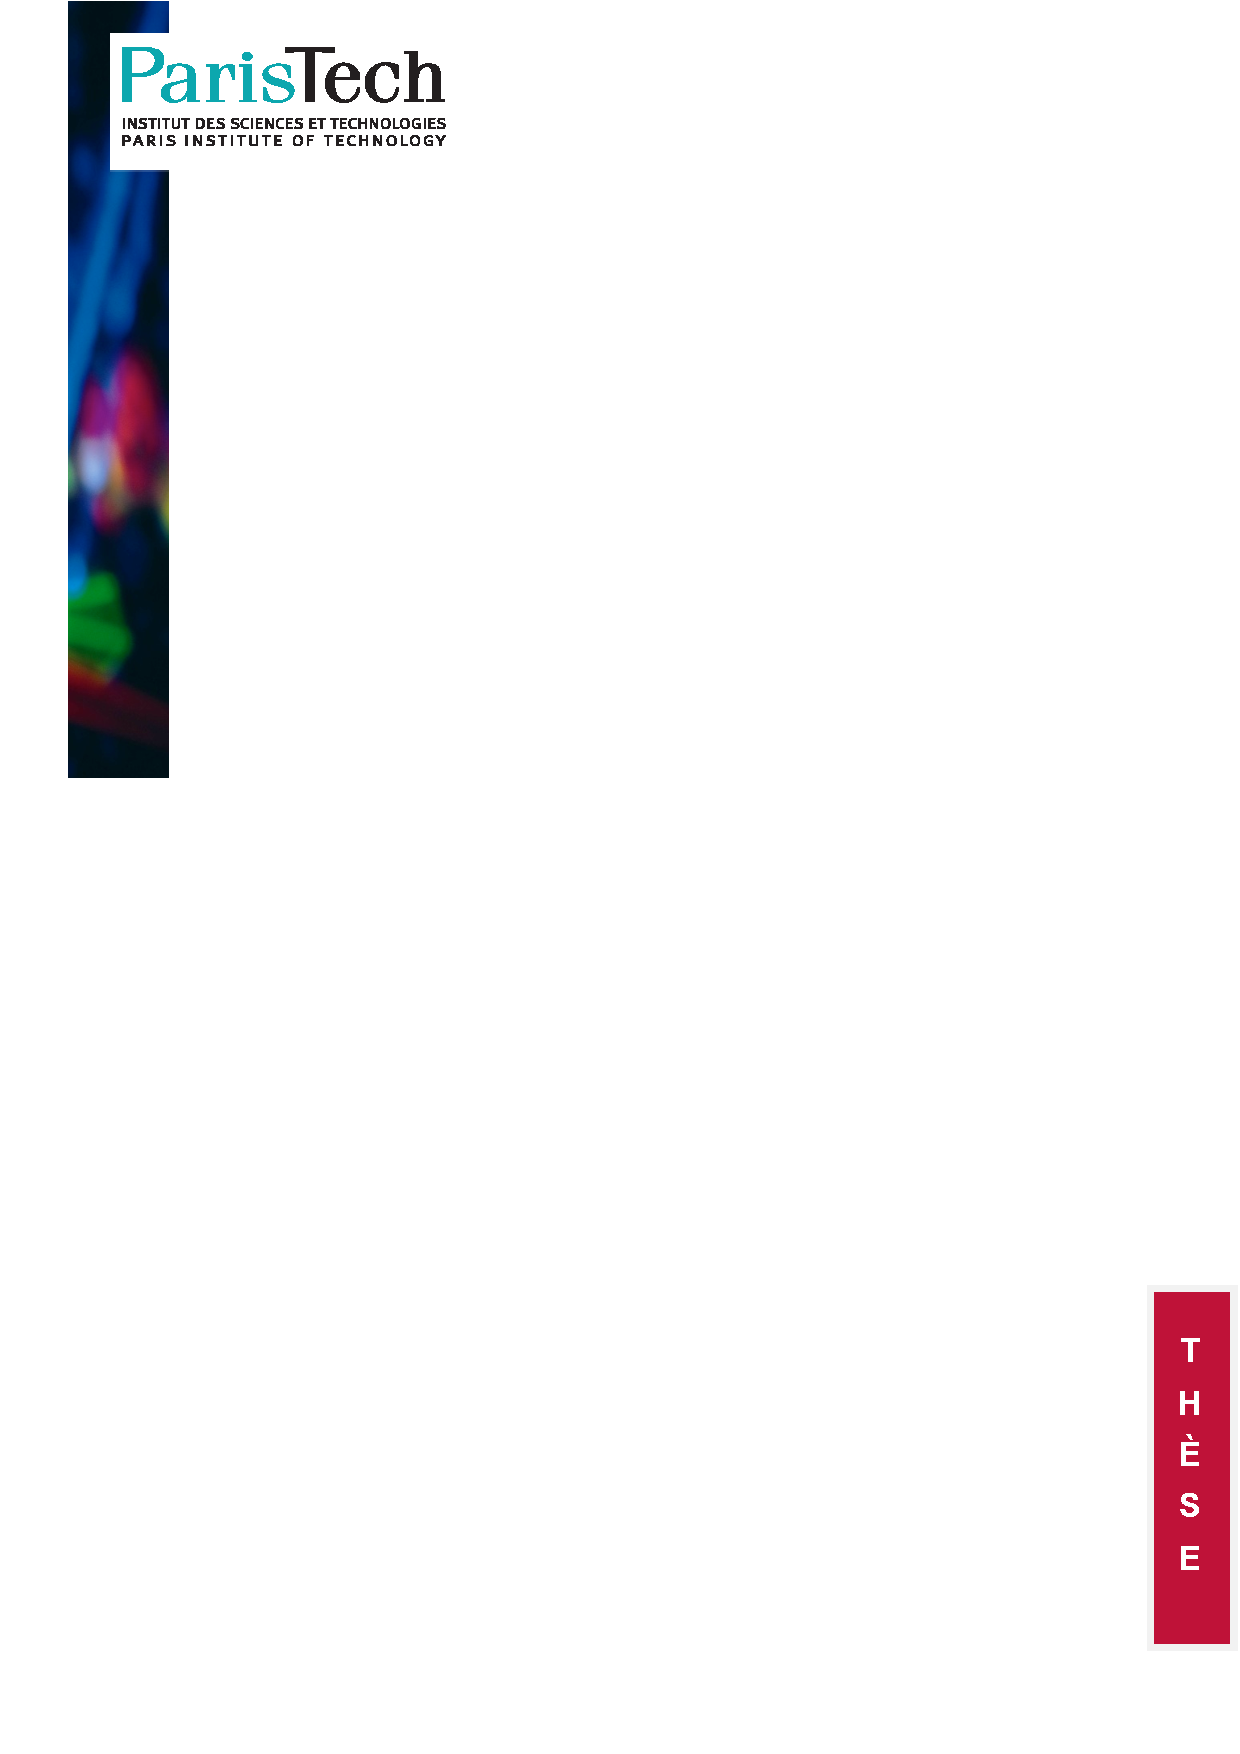
\includegraphics[height=\paperheight,width=\paperwidth]{cover_bg.pdf}
\else
	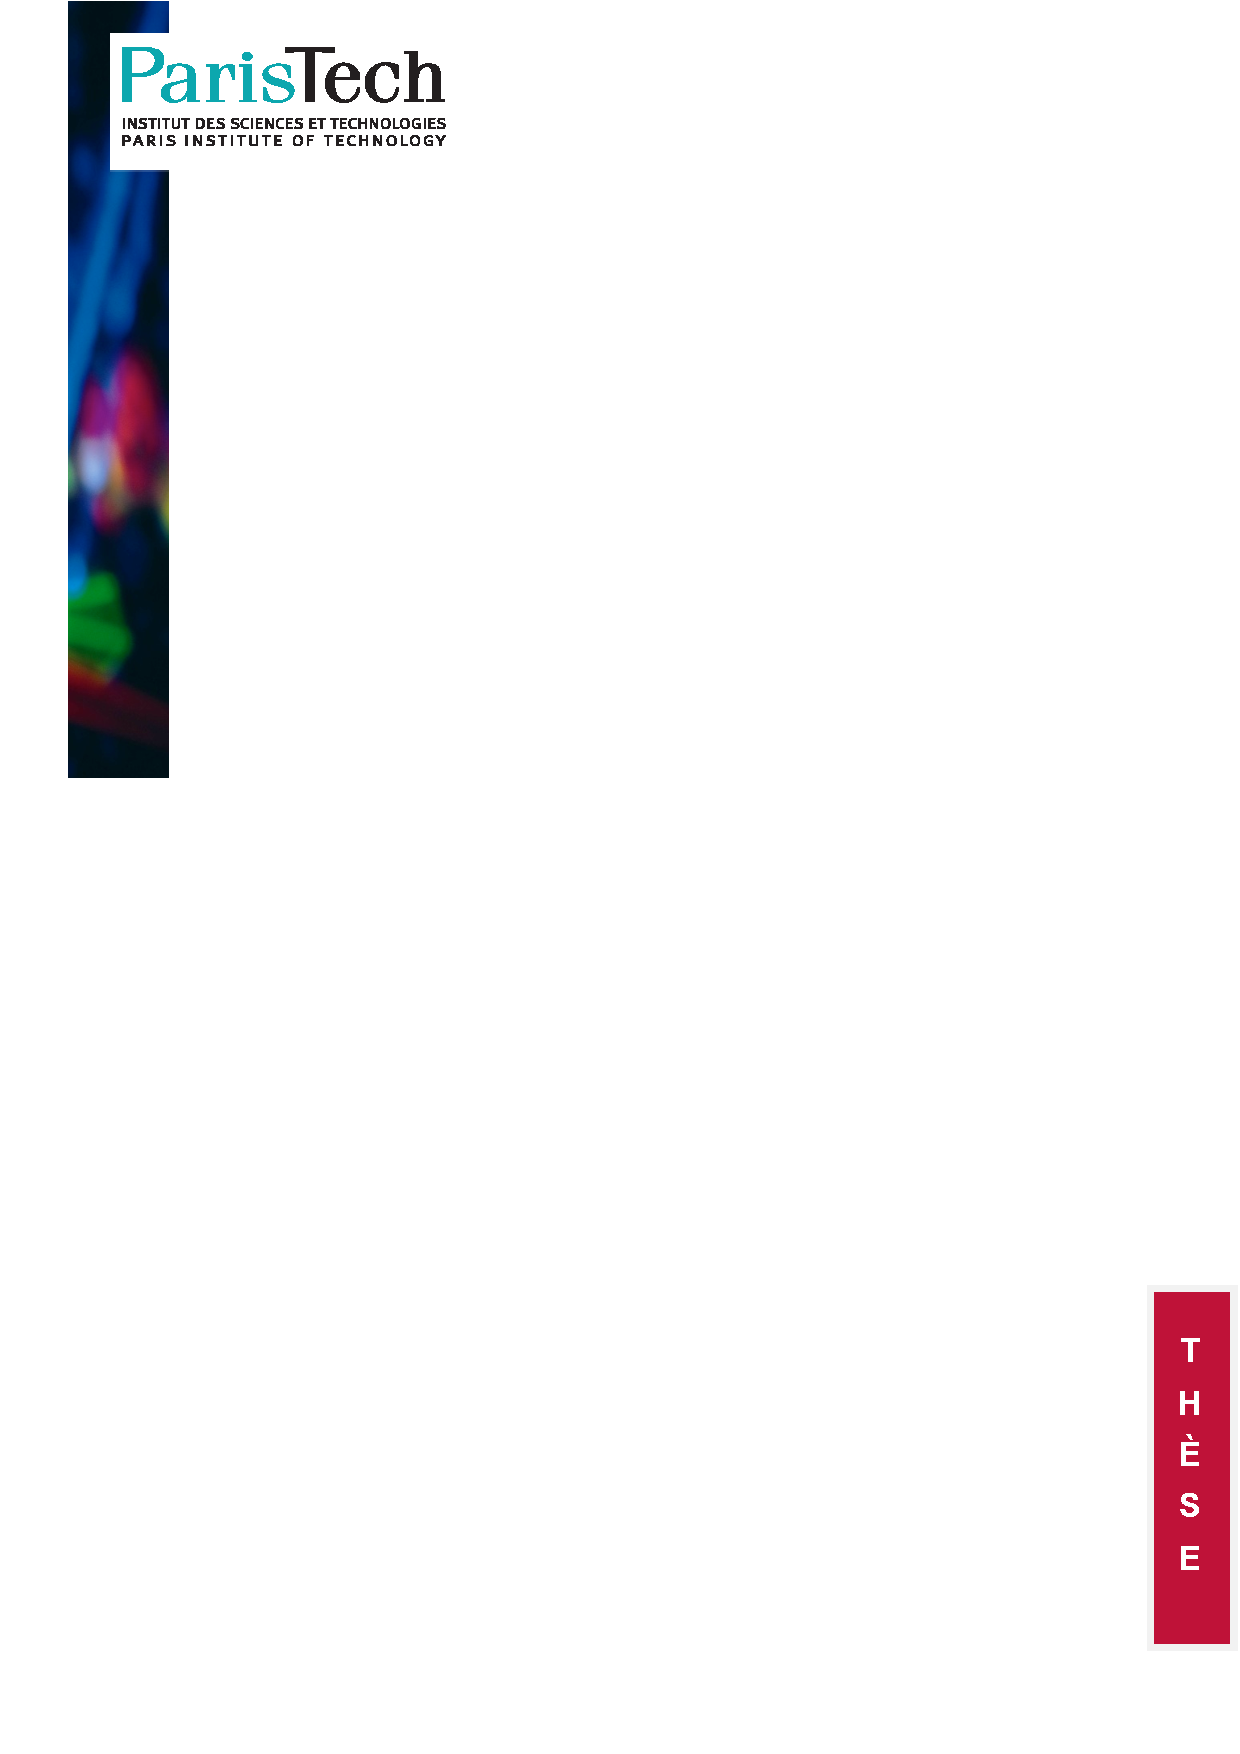
\includegraphics[height=\paperheight,width=\paperwidth]{cover_bg.pdf}
\fi}

\pagestyle{empty}

\begin{document}
\AddToShipoutPicture*{\BackgroundPic}
~

\begin{flushright}


\includegraphics[scale=0.45]{logo_TPT.pdf}

{\small {2015-ENST-00xx~~~~}}
\end{flushright}



%\vspace{0.cm}
\begin{center}
%



\includegraphics[scale=0.65]{logo_edite.pdf} \\
{\small {EDITE - ED 130}}


%
\vspace{.5cm}
%
%
%
%{\Large École doctorale \textnumero XX: texte}\\		% version une ligne
%{\Large École doctorale \textnumero XX:\\ texte}\\		% version deux lignes (changer les espaces en conséquence
%
%
%
\vspace{1.0cm}
%
%
%
{\LARGE {\bf Doctorat ParisTech}}\\
\vspace{1.1cm}
{\LARGE {\bf T H È S E}}\\
\vspace{0.5cm}
{\normalsize {\bf pour obtenir le grade de docteur délivré par}}\\
%
%
%
\vspace{.9cm}
%
%
%
%
{\LARGE {\bf TELECOM ParisTech}}\\
\vspace{0.6cm}
{\Large {\bf Spécialité Xxxx }}\\
%
%
%
\vspace{.8cm}
%
%
%
{\normalsize {\it présentée et soutenue publiquement par}}\\
\vspace{0.7cm}
{\Large {\bf Mainak JAS}}\\
\vspace{0.24cm}
{\normalsize le jour mois année}\\
%
%
%
\vfill
%
%
%
\textcolor[RGB]{191,18,56}{
\noindent
{\LARGE {\bf Advances in automating analysis of\\[.6cm]neural time series data}}\\
}
%
%
%
\vfill~\vfill
%
%
%
{\normalsize
\begin{tabular}{c}
Directeur de thèse:					{\bf Alexandre GRAMFORT}\\
Co-encadrement de la thèse:		{\bf Prénom NOM}
\end{tabular}
}
\end{center}
%
%
%
\vfill
%
%
%
\flushleft
\begin{minipage}{.9\textwidth}	% ou .91\textwidth si vous n'avez pas assez de place
{\bf Jury}\\
% Mme/M. Prénom NOM, Titre, Unité de recherche, Ecole 
{\bf Mme/M. Prénom NOM}, {\small Titre, Unité de recherche, Ecole}
	\hfill Fonction\\
{\bf Mme/M. Prénom NOM}, {\small Titre, Unité de recherche, Ecole}
	\hfill Fonction\\
{\bf Mme/M. Prénom NOM}, {\small Titre, Unité de recherche, Ecole}
	\hfill Fonction\\
{\bf Mme/M. Prénom NOM}, {\small Titre, Unité de recherche, Ecole}
	\hfill Fonction\\
{\bf Mme/M. Prénom NOM}, {\small Titre, Unité de recherche, Ecole}
	\hfill Fonction\\
{\bf Mme/M. Prénom NOM}, {\small Titre, Unité de recherche, Ecole}
	\hfill Fonction\\
{\bf Mme/M. Prénom NOM}, {\small Titre, Unité de recherche, Ecole}
	\hfill Fonction\\
{\bf Mme/M. Prénom NOM}, {\small Titre, Unité de recherche, Ecole}
	\hfill Fonction\\

\end{minipage}\\
%
%
%
\vspace{-.3cm}
%
%
%
{\centering
{\bf TELECOM ParisTech}\\
{\small école de l'Institut Mines-Télécom - membre de ParisTech}\\
{\tiny 46 rue Barrault 75013 Paris - (+33) 1 45 81 77 77 - www.telecom-paristech.fr}}
%
%
%
%
\end{document}
\begin{document}

\pagestyle{frontmatter}
\pagenumbering{roman}


\includepdf[]{build/coverpage}

\newpage\mbox{~}
\renewcommand{\familydefault}{\rmdefault}

\newcommand{\overbar}[1]{\mkern 1.5mu\overline{\mkern-1.5mu#1\mkern-1.5mu}\mkern 1.5mu}

\newcommand{\MATLAB}{\textsc{Matlab}}
\newcommand{\code}{\texttt}

\clearpage
\vspace*{\fill}
\begin{center}
\textit{This dissertation is dedicated to the memory \\ 
of my friend and colleague Venkat Raghav Rajagopalan (1993 -- 2017).}
\end{center}
\vspace*{\fill}

\chapter*{Acknowledgements}
First and foremost, my gratitude goes out to Alexandre Gramfort: my advisor, mentor and friend. Throughout these years, Alexandre has inspired me with his technical knowledge, his vision for long term impact, philosophy of open science, and wisdom. He introduced me to the welcoming and progressive MNE community which ultimately formed my collaboration network. It is these interactions that often led to new research projects and ideas. I thank Denis Engemann, a core contributor to MNE, who played a particularly pivotal role during these years as he shared his knowledge on the subtleties of MEG signal analysis and motivated me through our mini coding sprints. I thank Teon Brooks for collaborating with me on the BIDS project, Eric Larson for sharing his extensive open source experience, and other MNE team members: Jona Sassenhagen, Jean-Rémi King to name a few. I thank Pavan Ramkumar for being my longtime collaborator and friend, and for introducing me to the world of machine learning in neuroscience.

To my co-authors, I thank them for bearing with my whims and fancies. None of my projects would have been possible without the teamwork and efforts put in by them. I thank Umut for giving his time to answer my silly questions and work through the math with me. His experience in audio signal processing and probabilistic methods for machine learning has broadened my horizons. Jaakko's presence in the lab as an MNE engineer meant I spent less effort hunting bugs in MNE and more time on my thesis research (and playing tennis). Yousra has been not just a co-author but a friend, counsel, and the ``Einstein" when I was stuck with a particularly tricky bug. I thank Tom, whose expertise in scikit-learn and implementation skills were crucial during our projects. 

I thank my office mates for sharing the seminars, the Monday cakes, and the latest free food event. I thank my collaborators and friends at the Neurospin laboratory for inviting me to their social events and challenging me with new decoding problems. It is here that I made many like-minded international friends. To my French teacher Françoise and our Tuesday French lunch group, I am immensely indebted. It made life in France much easier for me. I could not have been productive without a vibrant social life which was made possible due to my friends. I thank Gabriela for the \textit{vernissage} events, Fosca for the bouldering evenings, David for organizing our weekly hiking trips, and Sokhany for making me see cooking in a new light. I thank my neighbors Anshuman and Bianca for the movie nights. I thank the \textit{desi} Indian community in France for making me feel home: Aakanksha for her amazing Indian cooking, Praveer for his jokes, Shabbir for his poetry, Pratheeban, Neeraj, Chirag, Sidharth, and Raghav. I did not realize how days in Paris flew by taking the metro to Gare du Nord with Raghav to grab the spiciest meal in town.

I thank my sister for her sense of humor and adventure. Finally, I thank my parents for their unconditional love.
% missing Johnny, Magdalena, Stanislas, Mathurin, Sophie

\today \\
Paris

\addcontentsline{toc}{chapter}{Acknowledgements}
\chapter*{Abstract}

Electrophysiology experiments has for long relied upon small cohorts of subjects to uncover statistically significant effects of interest. However, the low sample size translates into a low power which leads to a high false discovery rate, and hence a low rate of reproducibility. To address this issue means solving two related problems: first, how do we  facilitate data sharing and reusability to build large datasets; and second, once big datasets are available, what tools can we build to analyze them?

In the first part of the thesis, we introduce a new data standard for sharing data known as the Brain Imaging Data Structure (BIDS), and its extension MEG-BIDS. Next, we introduce the reader to a typical electrophysiological pipeline analyzed with the MNE software package. This will orient them towards the analysis process and the challenges that are often faced when building reproducible pipelines. We consider the different choices that users have to deal with at each stage of the pipeline and provide standard recommendations.

Next, we focus our attention on tools to automate analysis of large datasets such as those offered by the Human Connectome Project (HCP). We propose an automated tool to remove segments of data that are corrupted by artifacts. We develop an outlier detection algorithm based on tuning rejection thresholds with parameter search using Bayesian optimization. More importantly, we use the HCP data, which is manually annotated, to benchmark our algorithm against existing state-of-the-art methods. To our knowledge, this represents the first instance of reanalyzing the dataset using an independent stack of tools as used by the HCP consortium.

Finally, we use convolutional sparse coding to uncover structures in neural time series. The method we propose is inspired by similar algorithms in computer vision, where the goal is to learn the coefficients of a dictionary of atoms (traditionally sinusoidal or wavelets) but also the atoms themselves. We reformulate the existing approach as a \ac{MAP} inference to be able to deal with high amplitude artifacts and the heavy tailed noise distributions that is so common in neural time series. 

Taken together, this thesis represents an attempt to shift from slow and manual methods of analysis to automated, reproducible analysis.

\textbf{Keywords:} Automation, data sharing, reproducibility, sparse coding, outlier detection, representation learning, electroencephalography, magnetoencephalography
\addcontentsline{toc}{chapter}{Abstract}
\chapter*{Résumé}

Les expériences d'électrophysiologie ont longtemps reposé sur de petites cohortes de sujets pour découvrir des effets statistiquement significatifs d'intérêt. Toutefois, la faible taille de l'échantillon se traduit par une faible puissance, ce qui entraîne un taux élevé de fausses découvertes et, par conséquent, un faible taux de reproductibilité. Pour résoudre ce problème, il faut résoudre deux problèmes connexes: premièrement, comment faciliter le partage et la réutilisation des données pour créer de grands ensembles de données; et deuxièmement, une fois que de grands ensembles de données sont disponibles, quels outils pouvons-nous construire pour les analyser?

Dans la première partie de la thèse, nous introduisons une nouvelle norme de données pour le partage des données connue sous le nom de Brain Imaging Data Structure (BIDS), et son extension MEG-BIDS. Ensuite, nous présentons au lecteur un pipeline électrophysiologique typique analysé avec le progiciel MNE. Cela les orientera vers le processus d'analyse et les défis qui sont souvent rencontrés lors de la construction de pipelines reproductibles. Nous tenons compte des différents choix que les utilisateurs doivent faire à chaque étape du pipeline et nous formulons des recommandations normalisées.

Ensuite, nous concentrons notre attention sur les outils permettant d'automatiser l'analyse de grands ensembles de données tels que ceux offerts par le projet Connectome humain (HCP). Nous proposons un outil automatisé pour supprimer les segments de données corrompus par des artefacts. Nous développons un algorithme de détection d'anomalies basé sur le réglage des seuils de rejet avec recherche de paramètres par optimisation bayésienne. Plus important encore, nous utilisons les données HCP, qui sont annotées manuellement, pour comparer notre algorithme aux méthodes de pointe existantes. À notre connaissance, il s'agit du premier cas de réanalyse de l'ensemble de données à l'aide d'une pile d'outils indépendants utilisés par le consortium HCP.

Enfin, nous utilisons le codage convolutionnel à faible densité pour découvrir les structures des séries chronologiques neuronales. La méthode que nous proposons s'inspire d'algorithmes similaires en vision par ordinateur, où le but est d'apprendre les coefficients d'un dictionnaire d'atomes (traditionnellement sinusoïdaux ou ondelettes) mais aussi les atomes eux-mêmes. Nous reformulons l'approche existante comme une inférence MAP pour être en mesure de faire face aux artefacts d'amplitude élevée et aux distributions de bruits lourds qui sont si courantes dans les séries chronologiques neuronales. 

Ensemble, cette thèse représente une tentative de passer de méthodes d'analyse lentes et manuelles à des méthodes d'analyse automatisées et reproductibles.

\addcontentsline{toc}{chapter}{Résumé}

\tableofcontents
\listoffigures
\addcontentsline{toc}{chapter}{\listfigurename}
\listoftables
\addcontentsline{toc}{chapter}{\listtablename}
\listofalgorithms
\addcontentsline{toc}{chapter}{List of algorithms}
\printacronyms[include-classes=abbrev,name=Abbreviations, heading=chapter*]
\addcontentsline{toc}{chapter}{Abbreviations}

% for local table of contents
%\etocsettocstyle{\bigskip\hrule\medskip}{\medskip\hrule\vfill}

% for commenting
\newcommand{\mainak}[1]{\textcolor{red}{\textbf{mj:} #1}}

\chapter*{Sommaire (en Francais)}
\label{chapter:sommaire}
\pagestyle{mainmatter}
\pagenumbering{arabic}

Understanding the human brain is one of the most significant challenges of the 21st century. The human brain is arguably the most complex  organs of the human body, which performs a wide range of cognitive functions: from visual recognition to language understanding, speech, social interaction, and executive control. Pathologies of the brain are perhaps one of the biggest challenges for medicine today. Medical interventions and drugs for major infectious diseases are available today, and individuals can expect to live up to the mid 80s and even into their 90s. Yet, we still do not have a good grasp over most mental pathologies: Parkinson's, Alzheimer's, dementia, epilepsy to name a few. This is despite the fact that someone today who lives into their mid 80s has a 50\% chance of contracting Alzheimer's~\citep{alzheimer20162016}.

Our current understanding of the brain is a result of decades of concerted efforts across multiple disciplines ranging from molecular biology, genetics, physiology, cognitive and behavioral neuroscience, to statistics, computer science, and data science. A relatively new subfield here is brain imaging, also known as neuroimaging. Brain imaging refer to a set of technologies where  snapshots of the brain are taken. These snapshots can be static, as in the case of anatomical images from \ac{MRI}, or an evolving image, as in the case of \ac{fMRI}. The grand vision is to utilize them in hospitals to help diagnosis, in surgeries, in \acp{BCI}, or in research for neuroscientists to better understand the brain. 
In this thesis, we will focus our attention on measuring the electric currents and/or corresponding magnetic field from the brain, using electroencephalography, magnetoencephalography, and local field potentials. 
These methods have the property of possessing a high temporal resolution, which is particularly useful for extracting the temporal dynamics of brain signals.

In this thesis, I attempt to synthesize the lessons learned from analysing public neuroimaging data with open source software. To this effect, I participated in an international collaboration to create an \ac{MEG} standard for  \ac{BIDS}~\citep{niso2018meg}. I wrote the validator which helped create the MEG-BIDS compatible example datasets. As a contributor to MNE~\citep{gramfort2013meg}, I led an effort to write a tutorial paper which reanalyzes the Faces dataset~\citep{wakeman2015multi} for a reproducible group study. In the backdrop of the reproducibility and data sharing movement described in Sections~\ref{sec:reproducibility_crisis} and \ref{sec:intro_datasharing}, we started automating our pipelines which led us to develop a fully automated algorithm for artifact rejection and repair~\citep{jas2016automated, jas2017autoreject}. Finally, we develop algorithms to learn new undiscovered motifs automatically from neural time series data~\citep{jas2017learning}. 

The thesis is organized by chapters to highlight these four main  contribution areas: data sharing, reproducibility, automation for artifact detection, and automated data-driven motif discovery. An important aspect of this thesis is that these contributions led not only to publications in international conferences and journals, but also reproducible open source implementations and reusable datasets. A comprehensive list is given below.

\subsection*{Journal publications}
\bibentry{jas2017autoreject}\ \\ \\
\bibentry{jas2017mne}\ \\ (Pending revision at \emph{Frontiers in Neuroscience, Brain Imaging Methods})\ \\ \\
\bibentry{niso2018meg}

\subsection*{Conference publications}
\bibentry{jas2016automated}\ \\ \\
\bibentry{jas2017learning}

\subsection*{Workshop papers}
\bibentry{dengemann2015conc}\

\subsection*{Open source implementations}

\url{http://autoreject.github.io/} \\
\url{http://alphacsc.github.io/} \\
\url{http://mne-tools.github.io/mne-biomag-group-demo/}\\
\url{https://jasmainak.github.io/bids-validator/}

\subsection*{Datasets}

\url{https://openfmri.org/dataset/ds000248/}

In the French summary, I will introduce the context of the thesis followed by a brief summary of each of the four main contribution areas.

\section*{Electrophysiology}

\begin{figure}[htb]
\begin{center}
   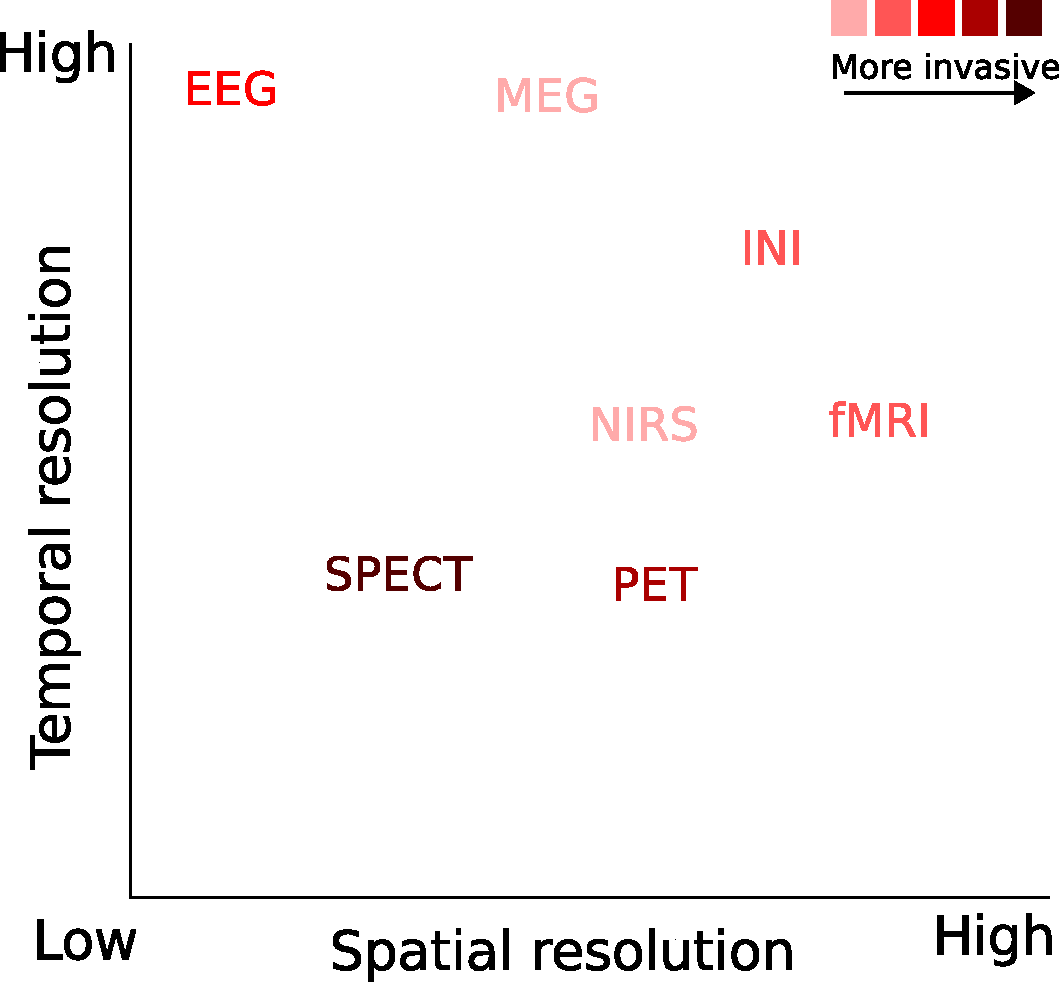
\includegraphics[width=0.6\linewidth]{figures/neuroimaging_methods.pdf}
\end{center}
   \caption[]{Various neuroimaging methods differ in terms of the information they measure. MEG=magnetoencephalography, EEG=electroencephalography, NIRS=near-infrared spectroscopy, PET=positron emission tomography, SPECT=single photon emission tomography, and INI=Inverse imaging, a method to speed up acquisition of fMRI images, ECoG=Electrocorticography, LFP=Local Field Potential.}
   \label{fig:sommaire:neuroimaging_methods}
\end{figure}

The study of electrical properties of the biological cells and tissues is known as electrophysiology. 
Biological tissues have electrical properties due to the presence of ions. Just as we can measure voltages in electrical appliances, it is possible also to measure these voltages in living tissues. 
Electrophysiological recording have the advantage of directly measuring the brain activity, as opposed to an indirect measure, which is for example the case in \ac{fMRI}.
Brain imaging techniques are characterized by their temporal and spatial resolution, \textit{i.e.,} the time scale at which it can measure brain activity, and also the accuracy of localizing the source of the activity. Figure~\ref{fig:sommaire:neuroimaging_methods} summarizes different neuroimaging methods with respect to their temporal and spatial resolution. In the case of \ac{fMRI}, as it measures the blood flow which is a slow response to neural activity, its temporal resolution cannot be high. 

There are a number of methods to measure the electrical potentials in the human body, the most well-known being perhaps \ac{ECG} which is used to measure the electrical activity of the heart. However, in our work, we will focus on only three which are relevant for studying the brain. Each of these methods produces a multivariate time series.

\paragraph{Electroencephalography: } \Ac{EEG} is a portable and non-invasive measurement technique invented in the 1920s that is  used in several contexts such as \acp{BCI}, monitoring and diagnosis, and in cognitive studies. 
In electroencephalography, an array of electrodes on an \ac{EEG} cap is placed on the scalp to measure the voltages with respect to a reference electrode. 
The voltage it measures is not the result of a single neuron but instead a result of the electrical activity of populations of  neurons. It has a high temporal resolution (in the order of \emph{ms}), however the spatial resolution is not so high.

\paragraph{Magnetoencephalography: } Any electric current is associated with magnetic fields as a consequence of Maxwell's theory. 
Therefore, the brain generates tiny magnetic fields which  wrap around the currents according to Maxwell's right hand thumb rule. The field is tiny ($\sim10^{-12}T$) compared to the earth's magnetic field ($\sim10^{-4}T$) and ambient magnetic noise ($\sim10^{-6}T$). Therefore, to measure it, one would need very sensitive electronics and heavy noise cancellation. The measurement itself is done in a magnetically shielded room made of three layers of metals. 
The sensors are superconducting coils which capture the magnetic flux. 
They are immersed in liquid Helium at very low temperatures (around 4 K), so as to lower any loss in signal due to resistance. A typical device contains two types of sensors: gradiometers and magnetometers. While the magnetometer measures the absolute magnitude of magnetic field, the gradiometer measures gradient of the field. \Ac{MEG} has the advantage that the skull does not deteriorate the signal quality as in \ac{EEG}.

\paragraph{\Ac{LFP}}
The Local Field Potential is the electric potential that is recorded in the extracellular space of the brain tissue. In contrast to \ac{EEG}, \ac{LFP} are recorded in depth, from within the cortical tissue and can therefore measure more localized populations of neurons. Small intracerebral electrodes are typically used to measure these potentials as opposed to large surface electrodes used in \ac{EEG}.

\section*{Context of the thesis}
This emerges out of the recent movements in reproducibility and data sharing in neuroimaging. It focuses on simplifying data analysis through better educational tools and automated methods to enable reproducible analysis in the age of big data.

\subsection*{The reproducibility crisis}
\label{sec:sommaire:reproducibility_crisis}
Even though thousands of papers are published every year about different aspects of the brain, our understanding of this complex organ has not scaled in proportion. A large part of the reason has been attributed to what is known as the reproducibility crisis~\citep{ioannidis2005most, simmons2011false, button2013power}. %Replication is closely related to the concept of reproducibility which refers to the idea that an experiment produces the same result when performed again under the same conditions. Replication is a stronger condition as it requires similar results or identical conclusion even if there are some minor variations in the experimental procedures. 
Progress in science rests on reproducible experiments. Reproducibility refers to the fact that the findings of an experiment can be regenerated independently if the code, data, and related software was provided. In many fields, however, a large fraction of experiments cannot be reproduced. In psychology, for instance, it was estimated that over half of the papers were not reproducible~\citep{open2015estimating}, and even those which could be reproduced tended to have a weaker effect size compared to the original studies. 

The reasons for unreproducible results can be numerous~\citep{baker20161}, some being: 1) confirmation bias, the tendency to selectively report only experiments that conform to the researcher's pre-existing beliefs, 2) ``p-hacking''~\citep{simmons2011false}, or the tendency to try multiple hypothesis to get a positive result, 3) publication bias or the absence of incentives to publish negative results~\citep{rosenthal1979file}, and 4) pressure to publish. There is now an accepted set of recommendations to address many of these issues: 1) pre-registering research plans to avoid confirmation bias and even report negative results, 2) correct for multiple comparisons, the most conservative method being the Bonferroni correction~\citep{dunn1961multiple}. 

Brain imaging has its own set of issues which can be linked to reproducibility crisis: 

% vul2009puzzlingly
% yendiki2014spurious

\begin{itemize}[noitemsep,partopsep=0pt]
\item \textbf{Power failure:} This is arguably one of the central issues in the reproducibility crisis today and has received by far the most attention. The statistical power of a study refers to the likelihood of discovering an effect of interest, given the sample size. Small sample sizes translate into underpowered studies which means that the chance of a false discovery is high. In order to discover the effect of interest, the study must be appropriately powered.
\item \textbf{Multiple comparison:} This is essentially a manifestation of ``p hacking'' that is a result of of the large number of voxels or time points in neuroimaging. For instance, in the famous dead salmon study~\citep{bennett2009neural}, a significant effect was found even if none was expected simply because the hypothesis testing (comparisons) was done over each voxel.
\item \textbf{Differences in software versions:} Changing software versions can lead to different results. For instance in the case of Freesurfer software, differences in volume were found in the range of $8.8\% \pm 6.6\%$~\citep{gronenschild2012effects}.
\item \textbf{Complex pipelines:} Neuroimaging pipelines involve a number of choices at each processing stage, and there is currently no consensus on how to choose the right pipeline. Often, these methodological choices are not even documented. It is estimated that there are almost as many unique pipelines as there are studies~\citep{Carp2012289}.
\item \textbf{Confounds:} There are several methodological confounds such as head movements~\citep{yendiki2014spurious}, anatomy differences, and changes in breathing rate and depth, which can lead to spurious correlations.
\end{itemize}

In Chapter~\ref{chapter:group_study} of the thesis, we will provide concrete guidelines on how to build processing pipelines for \ac{MEG}/\ac{EEG} data. Our contribution will touch upon the issue of complex pipelines, multiple comparison, and differences in software versions in the context of \ac{MEG}/\ac{EEG}. The issue of power failure can be alleviated through data sharing as I will discuss in the next section.

\subsection*{Data sharing}
\label{sec:sommaire:intro_datasharing}
Power failure is essentially a consequence of small datasets. In today's collaborative and data-driven scientific environment, data sharing is useful not only from the perspective of reproducibility but also to build datasets with large sample sizes. With large datasets, it would be possible to tease apart even subtle effects~\citep{smith2017statistical} that were not possible with smaller datasets. Data sharing is beneficial not just from the perspective of replication but also from an economic perspective. Rather than collect new data for every new hypothesis, researchers can now reuse known data for testing the validity of their hypotheses.

The benefits of data sharing can be traced back to Newton and his theory of gravitation~\citep{pointofview2013}. Before Newton had developed his theory, another English astronomer, John Flamsteed had been appointed by the king to observe the stars and produce accurate charts for navigation in the seas. Over a period of 40 years, Flamsteed created a detailed catalogue that tripled the number of entries in the previously used sky atlas. When the great comet of 1680 appeared in the sky twice in close succession, Flamsteed used his data to postulate that it was not two comets but in fact the same comet which first went towards the sun and then turned away from it. Newton initially opposed this theory, but later changed his mind as he gained access to Flamsteed's unpublished catalogue. The comet had indeed turned out to be an important benchmark for Newton's theory of gravitation.

It is hard to imagine in this day and age that a theory as fundamental as the laws of gravitation could have been data driven. Data sharing is fundamental not only to reproducible science, but also it forms the cornerstone for learning stronger models and benchmarking new algorithms. Consequently, in machine learning, recent breakthroughs have been powered by the increase in data sharing and computation. This includes the recent growth of deep learning~\citep{deng2009imagenet}, Q learning~\citep{watkins1992q, bellemare2013arcade}, natural language processing for language translation~\citep{halevy2009unreasonable}, speech recognition~\citep{paul1992design}, and even the mixture of experts model~\citep{jacobs1991adaptive} for IBM Watson~\citep{ferrucci2010building}. The maxim, ``more data beats a cleverer algorithm''~\citep{domingos2012few} has held up remarkably well across disciplines and over the ages.

Of course, neuroscientists are beginning to realize the importance of sharing data. In recent times, neural data has started being shared through international consortiums~\citep{van2013wu, ollier2005uk}, data repositories~\citep{poldrack2013toward, gorgolewski2015neurovault} and dataset papers in targeted journals. Yet, there is an unaddressed gap in terms of the ideal of data sharing and the practice of data sharing. Neuroimaging experiments are often very complicated, and it is not enough to share simply the data, but also the metadata and information regarding the experimental protocols in a well-structured format. 
In the absence of this information, shared data is not \emph{reusable} in the same way that uncommented and poorly structured, complicated programs are not useful even if shared publicly. 
There is not an accepted consensus in the community on the practices of sharing data and there is a need to establish a standard. 
In Chapter~\ref{chapter:group_study}, we will present a new standard known as the \ac{BIDS}, which is intended to address this gap. 
It is a collaborative effort between software developers and neuroscientists across various laboratories to establish a consensus on the standards and build tools to facilitate adoption of the standard.

\subsection*{Automation}
\label{sec:sommaire:automation}

Back in 2014, Nature published a bold article~\citep{hayden2014automated} which described a vision for the future of science: ``solving the problem of bringing McDonald's-like efficiency to scientists''. This would in turn lead to cheaper, more efficient and reliable research. While it goes on to describe many biology labs which are automating experiments, the benefits of automation in the neuroimaging community are yet to be widely recognized. Automation not only saves time but also makes the research more reproducible, as was noted in a recent guide to improve the transparency and reproducibility of neuroimaging research~\citep{gorgolewski2016practical}. The authors point out that manual work may seem easy at first, if the analysis has to be performed only once. However, this is not always the case as ``quite often in the course of a project, parameters are modified, subjects are changed, and processing steps need to be rerun. This is a situation in which having a set of scripts that can perform all of the processing steps automatically instead of relying on manual interventions can really pay off.'' As large datasets become more common in neuroimaging, automation will indeed become a necessity rather than a luxury.

In neuroimaging, there are in fact several avenues for automation:
\begin{itemize}[noitemsep,nolistsep,nosep]
\item \textbf{Reducing interactivity:} While interactive graphical user interfaces are excellent tools for browsing the data, they fall short when it comes to scaling up the analysis to tens and hundreds of subjects, which is necessary for a sufficiently powered study. 

\item \textbf{Parameter tuning:} Most algorithms, although scripted, still require hyperparameters to be tuned. These hyperparameters could be the number of ICA components to choose or the regularization parameters, and can vary from one subject to the next.
%This could be the number of trials to perform in an experiment, the number of components to select in a \ac{PCA} decomposition, or the regularization parameter in inverse solvers.
\item \textbf{Annotation and labeling:} A large fraction of neuroimaging data that is available is unlabeled or at best weakly labeled. This is because expert annotations are expensive, and cannot be crowdsourced. Automated tools based on unsupervised learning can play a major role in this regard.
\item \textbf{Quality control:} Currently, quality control is performed manually by inspecting the data to spot outliers. While data inspection cannot be overlooked, it can be performed more efficiently through automated documentation of data analysis and log reports such as the Jupyter notebook and the MNE web report~\citep{dengemann2015conc}. At the same time, advanced statistical trend analyses as in the Automated Statistician project~\citep{duvenaud2013structure} can be used for creating summaries.
\end{itemize}

There have been some steps taken in this direction, most notably the Neurosynth platform~\citep{yarkoni2011large} which facilitates large-scale meta analysis. Meta analysis typically combine results from multiple studies, and in this case, it is the brain activation maps from different studies which are combined by using machine learning methods. On the software side, the Freesurfer software package~\citep{dale-fischl-etal:99, fischl-serena-etal:99} provides a \code{recon-all} command that performs cortical segmentation automatically without any human intervention. In MNE, this philosophy is now being adopted starting with automated covariance estimation~\citep{engemann2015automated_new}.

In this thesis, we will consider an algorithm that automatically annotates artifacts in the data~\citep{jas2016automated, jas2017autoreject}. This is a first step that any \ac{MEG}/\ac{EEG} processing pipeline has to go through but it is often done manually. A reason for this is that existing algorithms are not designed to be \emph{transparent}. Since for most scientists, the key to new insights is an artifact-free dataset, they would rather spend extra effort in doing this manually rather than depend on a generic algorithm which is difficult to interpret. %However, this is problematic as it can lead to a selection bias: they might end up rejecting data segments which helps them confirm their hypothesis. 
Merely based on anecdotal reports, this process can take up to a week even for a moderately sized study of 10--20 subjects.

This is what led us to propose \emph{autoreject}, which we describe in Chapter~\ref{chapter:autoreject}. It is an algorithm which can be used to mark bad segments of the data. The key insight is that, often certain sensors in the device are intermittently corrupted rather than continuously. We validate our algorithm against 3 benchmarks on the \ac{HCP} dataset~\citep{larson2013adding} which is manually annotated with bad segments. In the process, our work also represents one of the first attempts at reanalyzing the MEG component of the HCP dataset.

\subsection*{Representation learning for data-driven discovery}
\label{sec:sommaire:representation_learning}
Since the invention of \ac{EEG} in the 1920s, scientists have discovered several different brain oscillation patterns such as alpha waves, K-complexes, and mu rhythms. The oscillations and interactions between them have served as biomarkers for different brain functions and pathologies. Alpha waves have been implicated in attention, K-complexes in sleep, and mu rhythm in motor activity. 

Considering the complexity of the human brain, clearly these waveforms represent only a fraction of the cognitive functions that the brain may perform. As a result of the wealth of data now available through the data sharing movement described in Section~\ref{sec:intro_datasharing}, the future neuroscientist will be able to mine such waveforms from large datasets. Imagine if neuroscientists had at their disposal a tool similar to Google Photos\footnote{\url{https://photos.google.com/}}. In the same way that Google Photos can automatically find faces and group photos, such tools will be able to find prototypical oscillations and cluster the data using them. Clicking on any of these waveforms would retrieve the data associated with them.

\begin{figure}[htb]
\begin{center}
   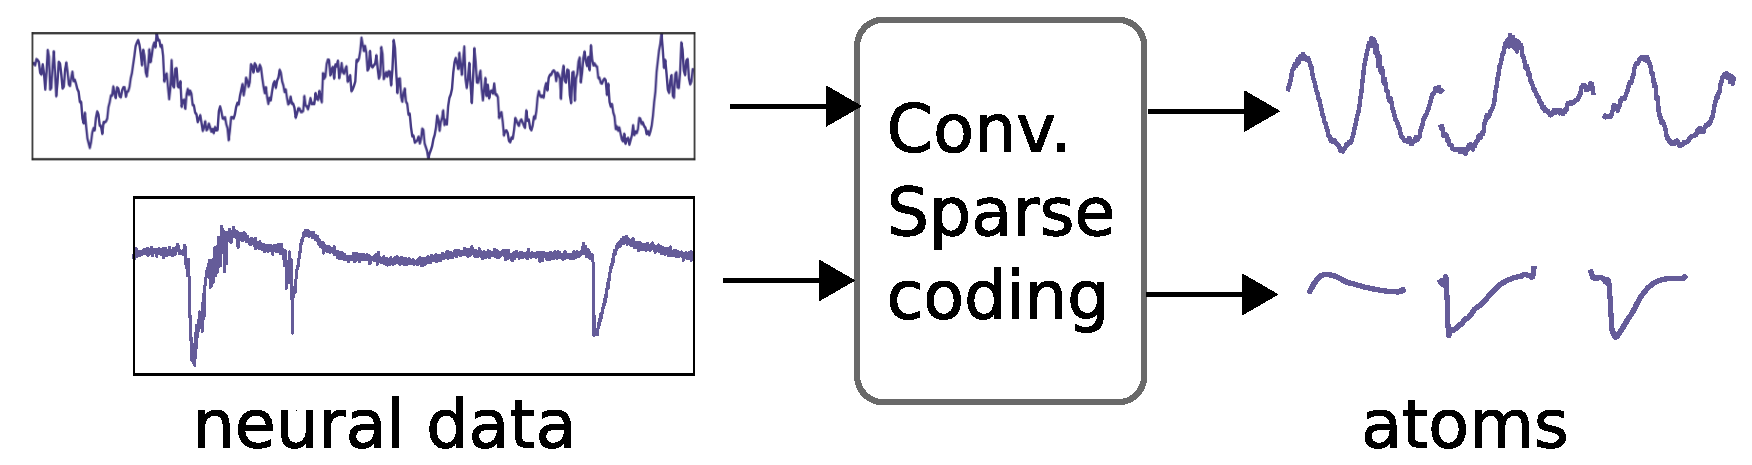
\includegraphics[width=0.85\linewidth]{figures/schema.pdf}
\end{center}
   \caption[]{An illustration of how Convolutional sparse coding can be used to automatically mine prototypical waveforms}
   \label{fig:sommaire:csc_schematic}
\end{figure}

However, photos are inherently different from neural data. First, neural data can be buried in noise and corrupted by high amplitude artifacts. Second, images are labelled owing to crowdsourced data as in the case of  Imagenet~\citep{deng2009imagenet}, but neural data is not. 
Expert annotations in the case of neural data are not easily available.
Finally, it is spatiotemporal data with different dynamics from the 3D world that photos capture. This is where \ac{CSC} can play a role by extracting prototypical features from the data, as shown in Figure~\ref{fig:csc_schematic}. It is an unsupervised algorithm from computer vision, which can learn shift-invariant dictionaries of prototypical waveforms (atoms) from the data using the convolution operations. For a more comprehensive background on \ac{CSC}, the reader may read Section~\ref{sec:background_dict_learning} later in this chapter.

\ac{CSC} algorithms do not approximate the signal using Fourier (or sinusoidal) basis. While this is the conventional technique for extracting signals buried in noise, the approximation can degrade the shape of the signal, which can be a biomarker in many clinical diseases~\citep{cole2017brain}. As an example, even with a large number of sinusoids from the Fourier basis, the edges of a square wave cannot be approximated well. Indeed, the imperfect approximation around such edges is what is often termed as ringing artifacts in signal processing contexts. Of course, transients can be better approximated using wavelets but it is clearly not sufficient for other shapes of data. Rather than fix the basis to be Fourier or wavelet, the \ac{CSC} approach is to learn \emph{both} the basis and the coefficients.

In our work presented in Chapter~\ref{chapter:alphacsc}, we extend conventional \ac{CSC} algorithms for heavy-tailed noise. We reformulate the optimization problem as a \ac{MAP} inference with an alpha-stable distribution to replace the reconstruction loss. Our results show that this kind of algorithm is robust to the presence of artifacts and can be used to uncover temporal structures from neural signals, even those involving nested oscillations.

\section*{Brain Imaging Data Structure (BIDS)}

\begin{figure}[htb!]
\begin{center}
   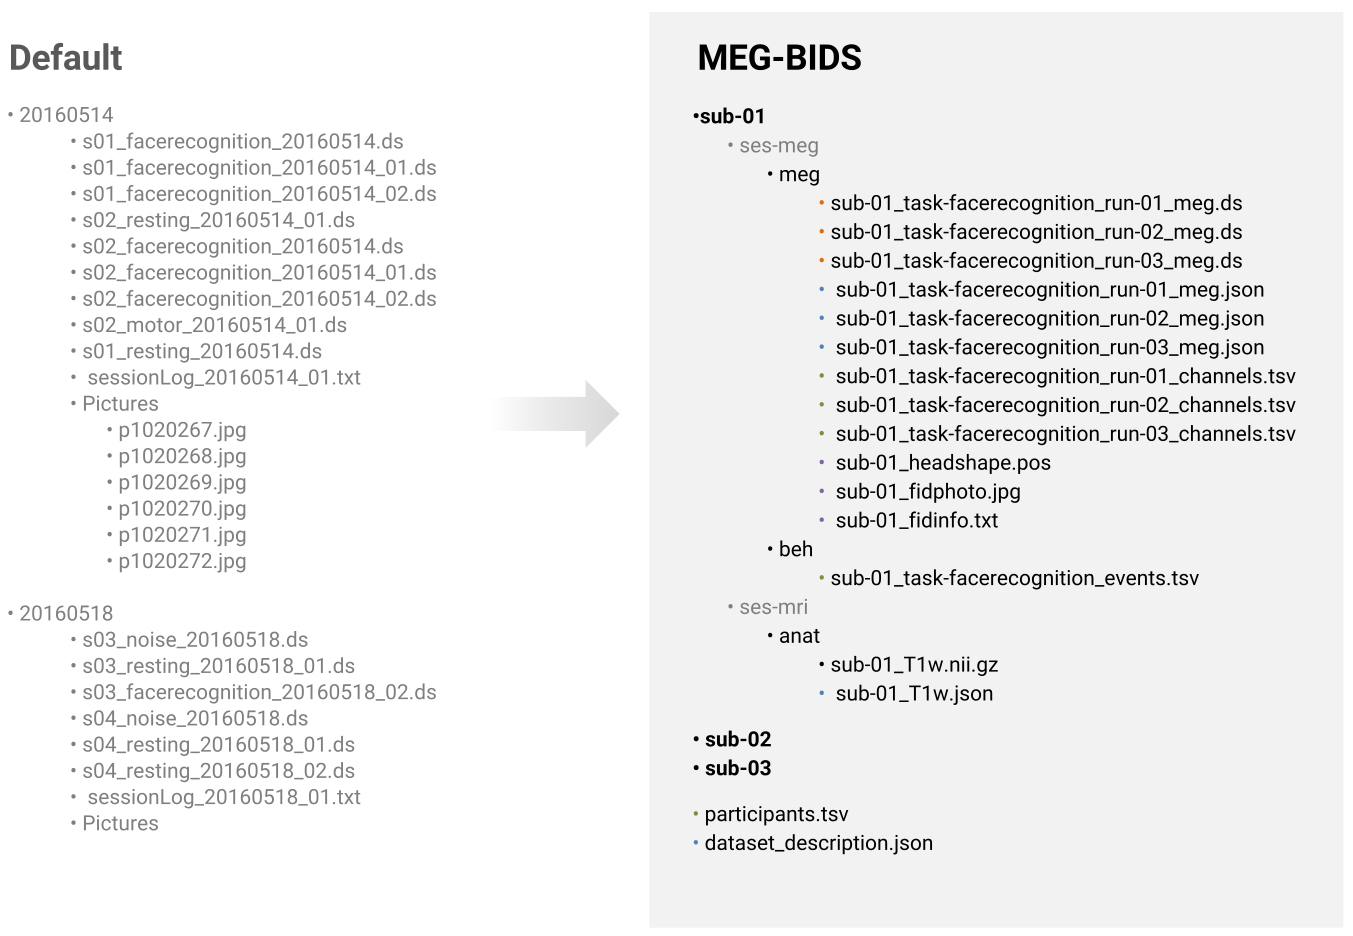
\includegraphics[width=\linewidth]{figures/bids_organization.png}
\end{center}
   \caption[]{BIDS-MEG data organization scheme: Left: a typical default data organization scheme where folders are organized by date of session and contain different runs for a given participant in a study. Right: BIDS-MEG organizes data per study, then participant (subject), followed by modality, then sessions and eventually, runs. Note the sidecar files that are present at all levels of the data hierarchy, and document conveniently the metadata contents.}
   \label{fig:sommaire:BIDS-MEG-organization}
\end{figure}
From the perspective of reproducibility, data sharing is of paramount importance. Sharing code by itself does not enable reproducibility if the accompanying data is not available, and expensive to acquire. Reanalysis of a dataset is however useful not just from the perspective of reproducibility but also for discovering new effects that were previously overlooked. At the same time, the more data is shared, the larger our sample sizes will be and this will enable us to conduct studies with higher statistical power. Indeed, low statistical power is one of the main reasons for the reproducibility crisis.

While data sharing in neuroscience is on the rise, the amount of data reuse is still limited. For example, since the release of the Human Connectome Project (HCP)~\citep{larson2013adding} MEG data in 2013, there have been very few instances of reusing this data. At the time of writing this thesis, we had only one or two documented cases~\citep{jas2017autoreject} of reusing the HCP data. Even in these cases, the effort has mostly been limited to reproducing results rather than testing new hypotheses. This clearly represents a gap between the ideal and the practice of data sharing. 

% Clearly, sharing data is not a panacea as the tools, skills and resources to process such large datasets is currently missing in typical laboratories. Perhaps the most important roadblock is standardization of metadata.

Neuroimaging experiments are often complicated involving different  cognitive tasks (auditory, visual, somatosensory \emph{etc.}), different acquisition parameters (sampling frequency, number of sensors and their location, measurement device \emph{etc.}), and population parameters (subject's gender, age \emph{etc.}). All of this metadata is necessary information to successfully reanalyze the data. Unfortunately, historically there has been a lack of consensus amongst different labs and industrial manufacturers as to what constitutes useful metadata. This points to the need for establishing standards. While on a first glance, this may appear to be unnecessary bureaucratic red tape, in fact standards exist in almost all facets of our life. 

Apart from the meta information that is stored with the data, the data itself is stored amongst one of 10--20 different file formats and at different stages of processing. While there have been some efforts previously to standardize data structures~\citep{gibson2009minimum, grewe2011bottom, stoewer2013singlefile, teeters2015neurodata, bigdely2016preparing}, it has not gained wide acceptability. Designing a new standard is tricky as it requires gaining a community consensus. At the same time it must strike the right balance between rigidity for efficiency and flexibility for adapting to future technologies. 

The \ac{BIDS} format~\citep{gorgolewski2016brain} is indeed designed with these considerations in mind. 
The standard involves a hierarchy of folders to describe the imaging technology used, the name of the subject, and the date of the experiment. 
At each level of hierarchy, files are accompanied by sidecar \code{json} files describing the metadata. 
A \code{json} file is an easy to parse text file that contains key and value pairs, so that it has the advantage of being machine and human readable at the same time. 
These files follow an \emph{inheritance principle}, that is, a field described in a \code{json} file in a higher level of the hierarchy will be automatically propagated downstream. 
The main BIDS specification is accompanied by extension specifications which describe specific aspects to describe different modalities.
At the same time, the standard does not exist in isolation.
The \ac{BIDS} consortium is also providing a growing ecosystem of tools to convert datasets into \ac{BIDS} compatible format as well as to validate data to conform to the standard. 

In this work, we presented a significant extension of \ac{BIDS} to support the specific aspects of \ac{MEG} data. \Ac{MEG}, as we know, provides direct measurement of brain activity with millisecond temporal resolution and unique source imaging capabilities. So far, \ac{BIDS} has provided a solution to structure the organization of \ac{MRI} data. Despite the lack of standard data format for \ac{MEG}, BIDS-MEG is a principled solution to store, organize and share the typically-large data volumes produced. It builds on \ac{BIDS} for \ac{MRI}, and therefore readily yields a multimodal data organization by construction. This is particularly valuable for the anatomical and functional registration of \ac{MEG} source imaging with \ac{MRI}. With BIDS-MEG and a growing range of software adopting the standard, the \ac{MEG} community has a solution to minimize curation overheads, reduce data handling errors and optimize usage of computational resources for data analysis. The standard also includes well-defined metadata to facilitate future data harmonization and sharing efforts, and extensions to other electrophysiological data modalities.

\clearpage
\section*{A reproducible M/EEG group study}

\begin{figure}[t]
  \centering
  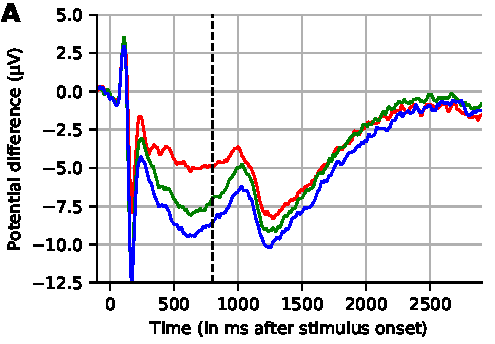
\includegraphics[width=0.7\linewidth]{figures/grand_average_highpass-NoneHz.pdf}\\
  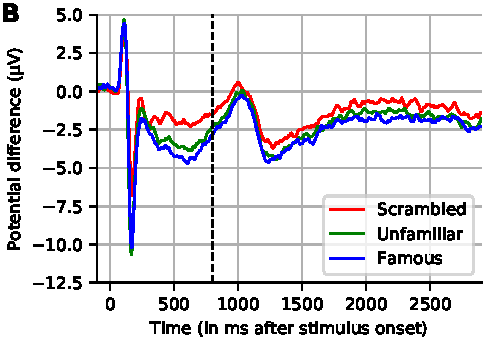
\includegraphics[width=0.7\linewidth]{figures/grand_average_highpass-1Hz.pdf}
\caption[]{Grand averaged evoked response across 16 subjects for channel EEG065.
(A) No highpass filter. (B) Highpass filtered at 1.0 Hz. Note that, similar to (A), the results reported by \cite{wakeman2015multi} (dashed line at 800 ms indicates where their plot stopped) show large drifts, but these return to near-baseline levels toward the end of a sufficiently long interval (here, 2.9 seconds) even without applying a highpass filter.}
\label{fig:sommaire:grand_average}
\end{figure}  

In the previous section, we discussed how data sharing can be facilitated using the \ac{BIDS} for \ac{MEG}. This is taking us one step closer to the goal of reproducibility. However, reproducibility is not achieved by merely sharing more data with the hope that this will solve all problems. As noted in \citet{baker20161}, one of the best solutions to foster reproducible science is not a technical one, but an educational one. This is of course true for statistics, where there is an urgent need to clarify and educate researchers about the statistical tools required in neuroscience. But it is now increasingly important also for academic software.

In recent years, free academic toolboxes have gained increasing prominence in \ac{MEG} analysis as a means to disseminate cutting edge methods, share best practices between different research groups and pool resources for developing essential tools for the \ac{MEG} community. Teaching events are regularly held around the world where the basics of each toolbox are explained by its  developers and experienced power users. There are however, knowledge gaps that need to be addressed. First, most teaching examples only show analysis of a single ‘typical best’ subject whereas most real MEG studies involve analysis of group data. It is then left to the researchers in the field to figure out for themselves how to make the transition and obtain significant group results. Secondly, we are not familiar with any examples of fully analyzing the same group dataset with different academic toolboxes to assess the degree of agreement in scientific conclusions and compare strengths and weaknesses of various analysis methods and their independent implementations.

To address this very issue, a workshop was organised by the lead developers of six most popular free academic MEG toolboxes at Biomag 2017. This work is a follow up to the workshop, which presents the contribution of the MNE software team, and will be published in \emph{Frontiers in Neuroscience, section Brain Imaging Methods}. This study presents the results obtained by the reanalysis of an open dataset from \citet{wakeman2015multi} using the MNE software package. The analysis covers preprocessing steps, quality assurance, sensor-space analysis of evoked responses, source localization, and statistics in both sensor and source space. Results with possible alternative strategies are presented and discussed at different stages such as the use of high-pass filtering versus baseline correction, tSSS versus \ac{SSS}, the use of a minimum norm inverse versus \ac{LCMV} beamformer, and the use of univariate or multivariate statistics. An example of such a reanalysis figure is shown in Figure~\ref{fig:sommaire:grand_average} which shows the evoked response for one EEG sensor.

This aims to provide a comparative study of different stages of \ac{MEG}/\ac{EEG} analysis pipeline on the same dataset, with open access to all of the scripts necessary to reproduce this analysis.

\clearpage

\section*{Automated artifact rejection for M/EEG}

\begin{figure}[t]
	\centering
	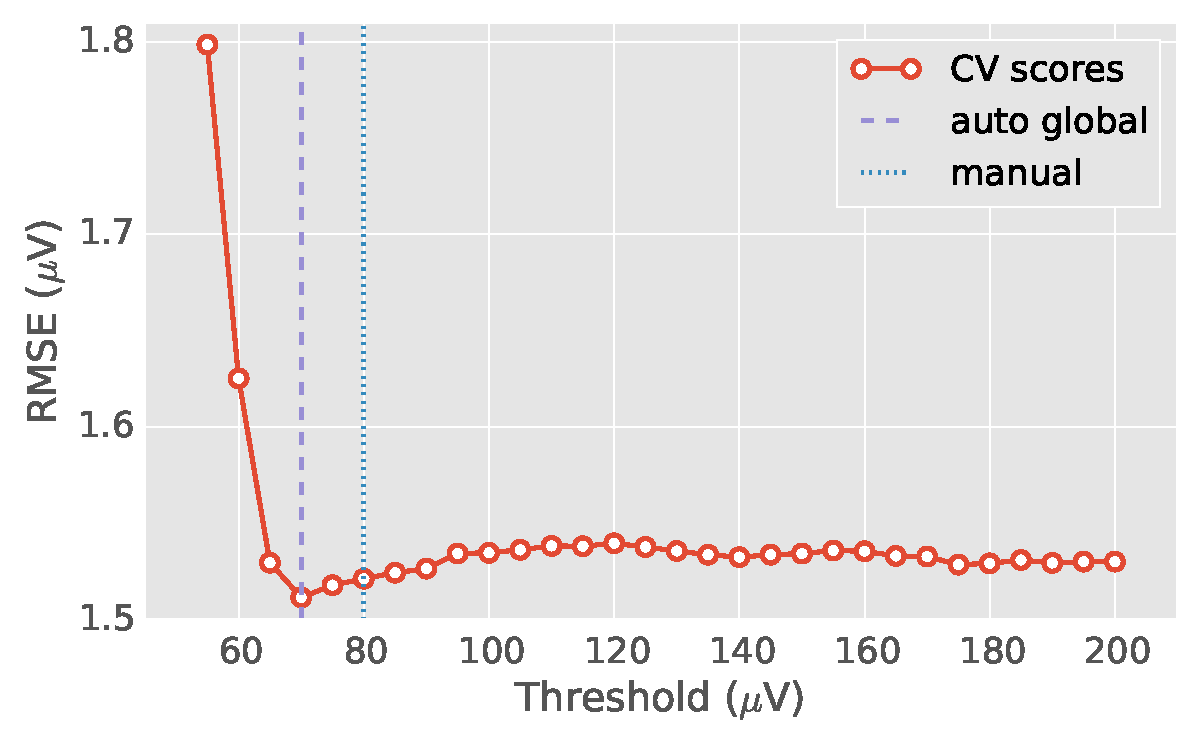
\includegraphics[width=0.8\linewidth]{figures/figure1.pdf}
    \caption[]{Cross-validation error as a function of peak-to-peak rejection threshold on one EEG dataset. The root mean squared error (RMSE) between the mean of the training set (after removing the trials marked as bad) and the median of the validation set was used as the cross-validation metric (Section~\ref{sec:auto_global}). The two insets show the average of the trials as ``butterfly plots" (each curve representing one sensor) for very low and high thresholds. For low thresholds, the RMSE is high because most of the trials are rejected (underfit). At high thresholds, the model does not drop any trials (overfit). The optimal data-driven threshold (\emph{autoreject, global}) with minimum RMSE is somewhere in between. It closely matches the human threshold.}
    \label{fig:sommaire:cross_val}
\end{figure}

In the previous section, we discussed the reproducibility challenges when performing group studies in \ac{MEG} and \ac{EEG}. One way to improve reproducibility is automation. and we briefly touched upon an algorithm for automating detection of bad data segments, known as \emph{autoreject}.

%copy pasted abstract below
In this section, we will present this algorithm which rejects and repairs bad trials in \ac{MEG} and \ac{EEG} signals. Annotating bad segments in the data is perhaps one of the most time consuming aspects of data processing in electrophysiology. Currently, it is either done manually, or using automated black-box algorithms. The manual approach is often subjective with often no clear consensus on what constitutes a corrupted data segment. Therefore, reanalysis is not only manually demanding but can also lead to problems in reproducibility. On the other hand, the automated methods are controlled by parameters that are not straightforward to tune. In the case of failure, it is not always obvious what caused the method to fail and how it can be corrected. As a result, one is left with no choice but to exclude the data from further analysis.

This led us to develop a method based on design choices motivated by ease of interpretation and diagnosis. The method we propose capitalizes on cross-validation (Figure~\ref{fig:sommaire:cross_val}) in conjunction with a robust evaluation metric to estimate the optimal peak-to-peak threshold--a quantity commonly used for identifying bad trials in \ac{MEG}/\ac{EEG}. This approach is then extended to a more sophisticated algorithm which estimates this threshold for each sensor yielding trial-wise bad sensors. Depending on the number of bad sensors, the trial is then repaired by interpolation or by excluding it from subsequent analysis. For efficiency reasons, we use Bayesian optimization which is a well-known technique for hyperparameter optimization. All steps of the algorithm are fully automated thus lending itself to the name \emph{autoreject}. Crucially, the algorithm is even able to deal with sensors that are locally corrupted, which is quite often the case for \ac{EEG} data.

In order to assess the practical significance of the algorithm, we conducted extensive validation and comparisons with state-of-the-art methods on four public datasets containing \ac{MEG} and \ac{EEG} recordings from more than 200 subjects. The comparisons include purely qualitative efforts as well as quantitatively benchmarking against human supervised (Figure~\ref{fig:sommaire:hcp_scatter}) and semi-automated preprocessing pipelines. The algorithm allowed us to automate the preprocessing of \ac{MEG} data from the \ac{HCP} going up to the computation of the evoked responses. The automated nature of our method minimizes the burden of human inspection, hence supporting scalability and reliability demanded by data analysis in modern neuroscience.


\begin{figure}[htb!]
    \centering
    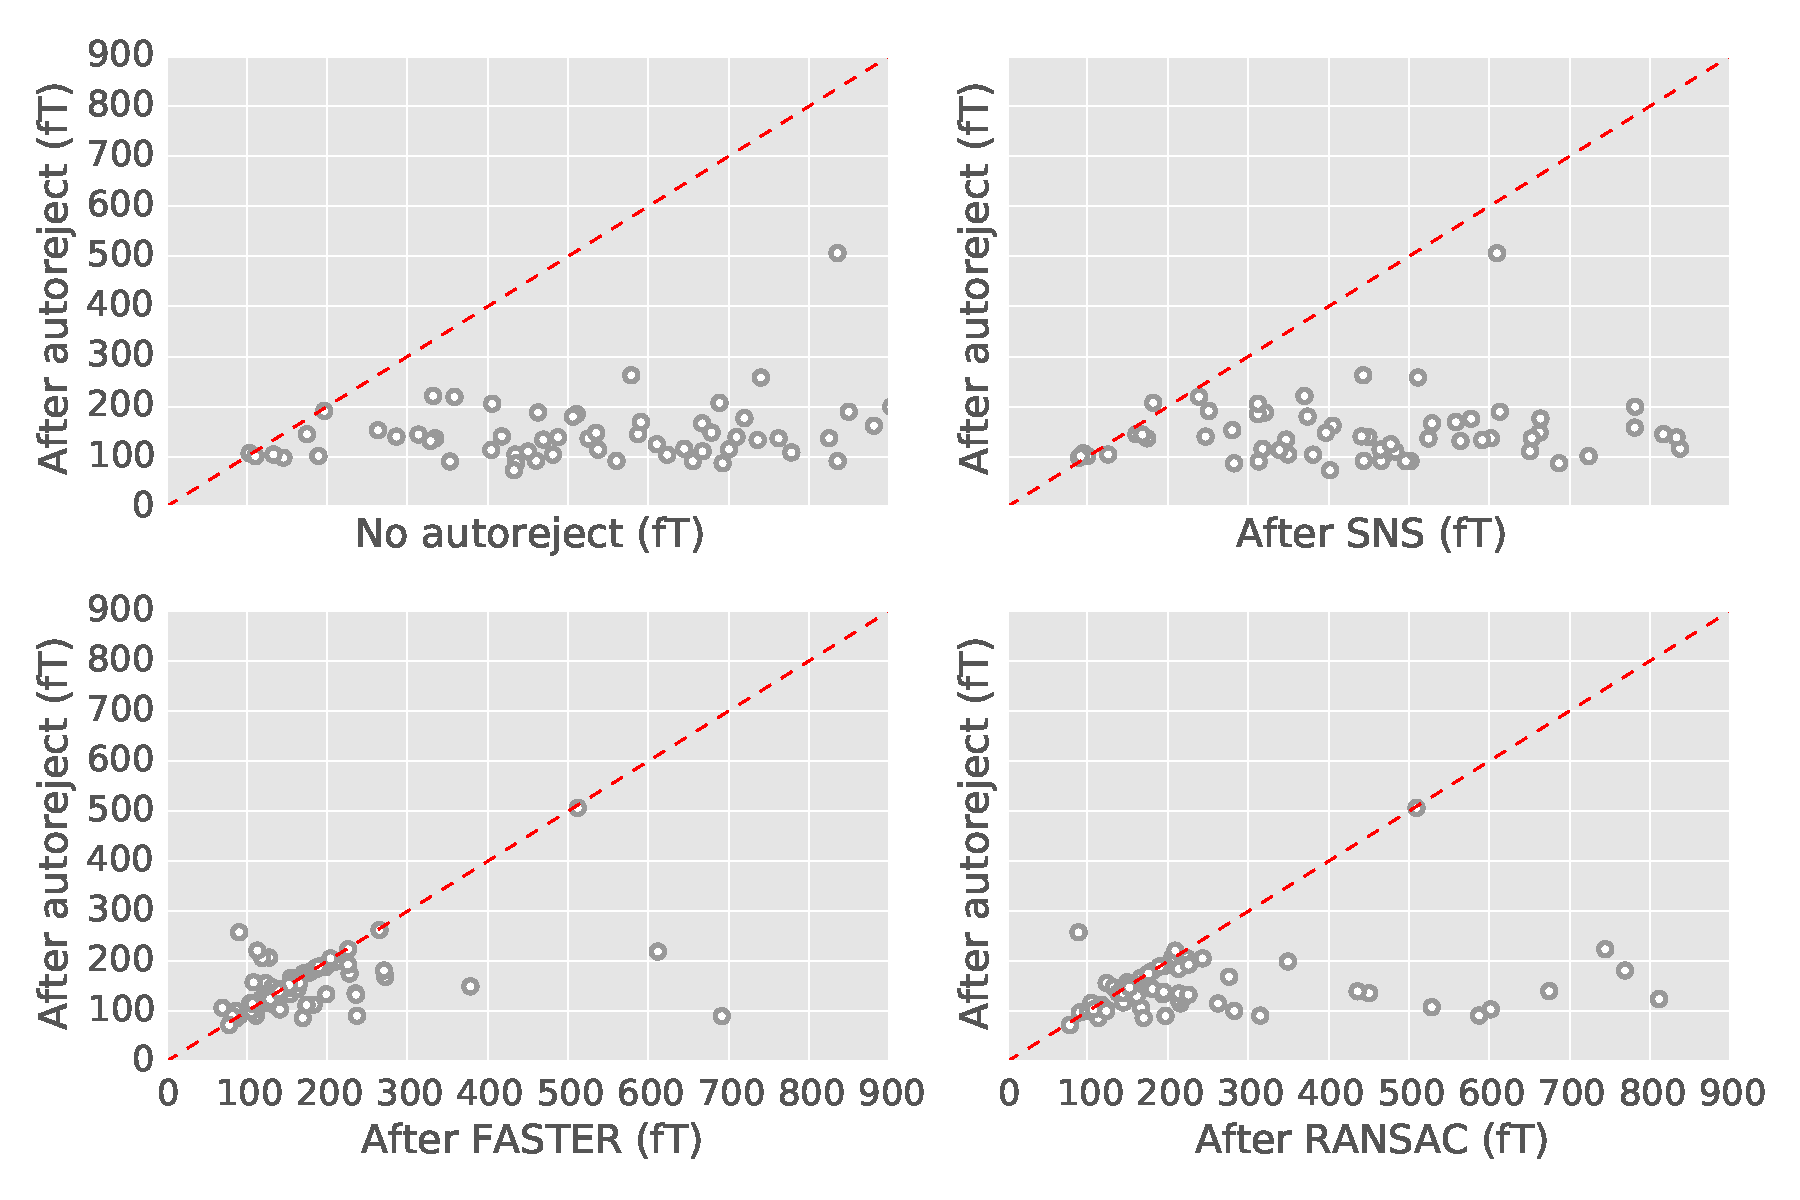
\includegraphics[width=\linewidth]{figures/figure4.pdf}
    \caption[]{Scatter plots for the results with the HCP data. For each method, the $\infnorm{\cdot}$ norm of the difference between the HCP ground truth and the method is taken. Each circle is a subject. (A) \textit{autoreject (local)} against no rejection, (B) \textit{autoreject (local)} against Sensor Noise Suppression (SNS) (SNS), (C) \textit{autoreject} against FASTER, (D) \textit{autoreject (local)} against RANSAC. Data points below the dotted red line indicate subjects for which \textit{autoreject (local)} outperforms the alternative method.}
    \label{fig:sommaire:hcp_scatter}
\end{figure}

\clearpage
\section*{Temporal representation learning}

So far, we studied automation in neuroimaging with the objective of enabling scalable data analysis and reproducibility. While  reproducibility and large-scale data analysis allow us to consolidate upon existing studies, \emph{per se} they are not tools to uncover new and interesting phenomena. In this chapter, we will explore this dimension of automation using what is known as \emph{representation learning}.

Representations are the building blocks of signal processing. It is quite easy to convince ourselves of this fact, if we simply use a Fast Fourier Transform (FFT) to filter data. When we are using an FFT, we are in effect, decomposing the signal into a sum of sinusoids of varying frequencies. If we are interested in a time-frequency analysis, a common choice of representation for neurosience signals consists in using Morlet wavelets.

Traditionally, the choice of representation has been mainly driven by analytical concern and ease of mathematical manipulation. However, the recent surge of deep learning has ignited an interest in data-driven representations. It is because good representations  that compactly capture the properties of the data are essential for efficient and accurate learning systems. In computer vision, for instance, handcrafted features such as SIFT~\citep{lowe1999object} and GIST descriptors~\citep{oliva2001modeling}, Deformable Parts Model (DPM)~\citep{felzenszwalb2010object}, Histogram of Oriented Gradient (HOG)~\citep{dalal2005histograms} \emph{etc.} had been the norm, before it was realized that unsupervised learning and autoencoders performed much better.

Today, unsupervised learning is used as a first step for a supervised learning task in computer vision. Representation learning, by itself, is perhaps not as interesting, except for diagnostic visualizations in deep learning~\citep{zeiler2014visualizing}. Despite this, there has always been an interest in understanding representations in the human brain (visual system particularly), as it was thought that this would help us build better learning systems. One of the pioneers in this area of research is Bruno Olshausen, whose work on dictionary learning~\citep{olshausen1996emergence} demonstrated that Gabor patches are indeed fundamental to natural images, similar to the ones that Hubel and Wiesel~\citep{hubel1962receptive, marcelja1980mathematical} found in the cat visual cortex, and to what is used in GIST features. Barring this line of studies, the learned representation itself is not considered as meaningful as performance metrics like the prediction score or reconstruction loss. However, in the case of neural signals, we realized that this is not the case and the fidelity of the representation is in itself interesting. Indeed, the shape of the signal is a crucial biomarker in many clinical applications for neuroscience~\citep{cole2017brain}. 

A parallel development in the field of neuroimaging has been the rise in interest for learning prototypical shapes which are shift invariant~\citep{jost2006motif, barthelemy2013multivariate, brockmeier2016learning, hitziger2017adaptive}. It is motivated by the fact that existing approximations using the Fourier basis often distorts the signal. There is, for example, a debate regarding the type of filters that should be used (See Section~\ref{sec:group_study_temporal_filtering} and \cite{widmann2015digital,parks1987digital,ifeachor2002digital, gotz-etal:15}). 
Even though some success has been reported
with these algorithms in neuroimaging, they are limited in applicability due to their heuristic nature.
Remarkably, there has been so far very little cross-pollination of ideas between the computer vision and neuroimaging communities on these sparse coding aspects. 
Our work is an attempt to bridge this gap. 
We propose a model which builds upon existing shift-invariant sparse coding models to be able to handle heavy-tailed noise and artifacts. It assumes positivity of the coefficients to account for the fact that an atom does not change polarity over time. 

Our model is a novel probabilistic \ac{CSC} model for learning shift-invariant atoms from unprocessed neural time series data containing
potentially severe artifacts.
In the core of our model, which we call $\alpha$CSC, lies a family of heavy-tailed
distributions called $\alpha$-stable distributions. We develop a novel, computationally efficient Monte Carlo
expectation-maximization algorithm for inference. The maximization step boils down to a weighted
\ac{CSC} problem, for which we develop a computationally efficient optimization algorithm.

In our work, we rigorously evaluate the computational efficiency of our algorithm against the competing benchmarks. Because the \ac{CSC} problem is non-convex, the optimization procedure involves nested loops and theoretical analysis often falls short in dealing with the complexity of non-convex functions. 
The optimization procedure is nested as the problem is convex when one of the variables is fixed: the atoms or the activations. The outer loop alternates between these two variables while the inner loop learns them when the other is fixed. An experimental approach, while challenging, is not completely out of reach. The final result depends on the initialization, and therefore algorithms can be compared only if they are tested for many different random seeds and their results averaged. Our qualitative analysis also goes beyond the narrative of verifying the existence of known waveforms to uncovering more complex structures in the data.

Our results
show that the proposed algorithm achieves state-of-the-art convergence speeds. Besides, $\alpha$CSC is
significantly more robust to artifacts when compared to three competing algorithms: it can extract
spike bursts, oscillations, and even reveal more subtle phenomena such as cross-frequency coupling
when applied to noisy neural time series.

\begin{figure}[t]
    \centering
     \subfigure[$K=10$, $L=32$.]{
     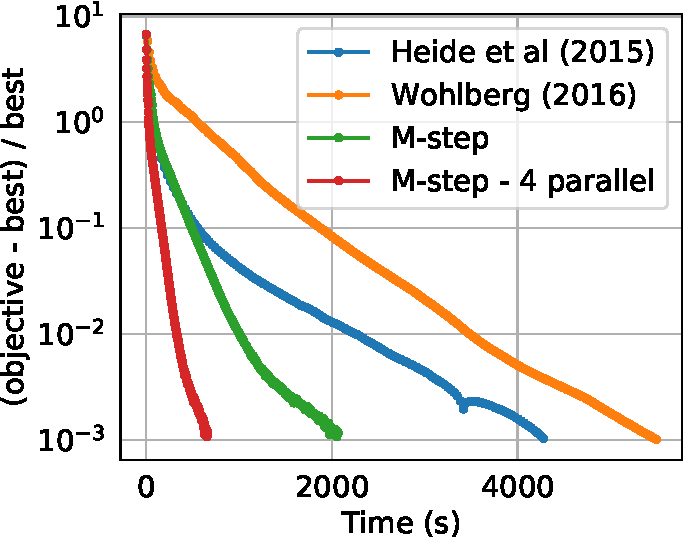
\includegraphics[width=0.5\linewidth]{figures/relative_10_32.pdf}} \\
     \subfigure[Time to reach a relative precision of 0.01.]{
     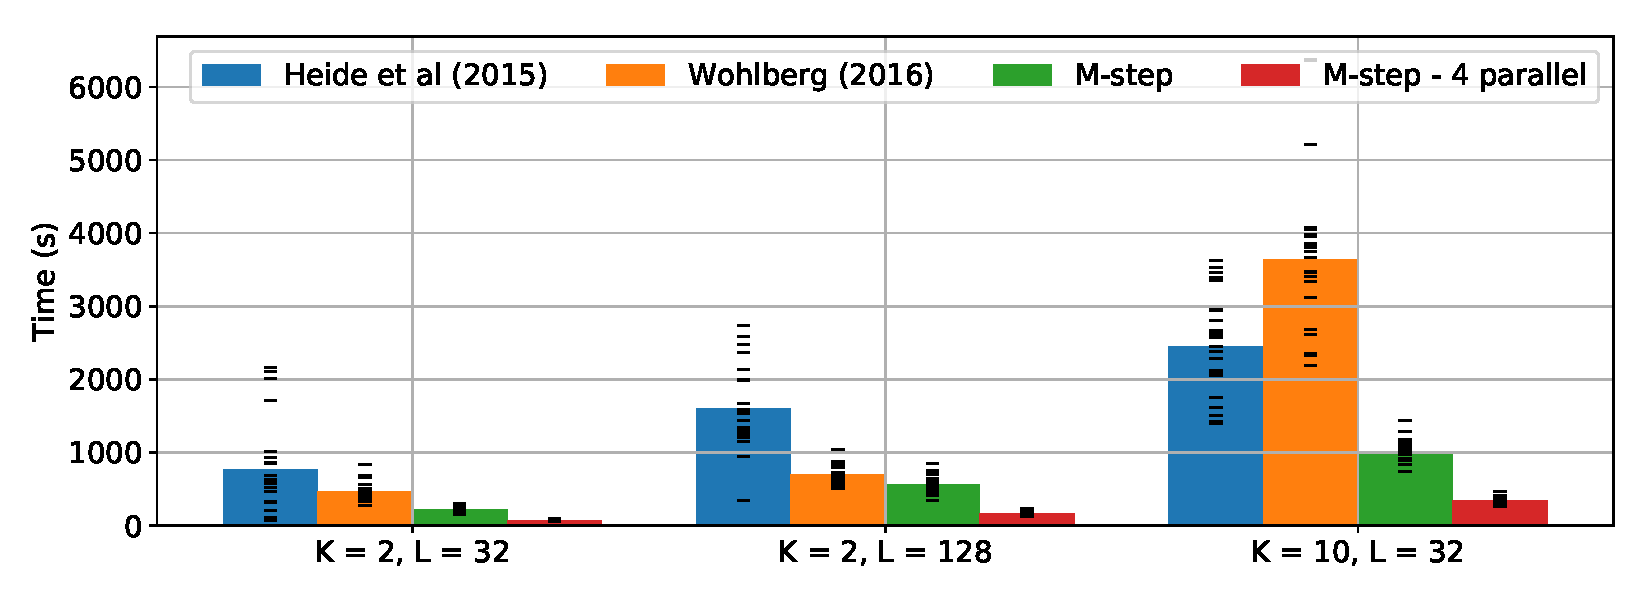
\includegraphics[width=\textwidth]{figures/bar_plot.pdf}}
    \caption[]{Comparison of state-of-the-art methods with our approach. (a)~Convergence plot with the objective function relative to the obtained minimum, as a function of computational time. (b)~Time taken to reach a relative precision of $10^{-2}$, for different settings of $K$ and $L$.  }
    \label{fig:sommaire:convergence}
\end{figure}

\begin{figure}[b]
    \centering
             \subfigure[LFP spike data from \cite{hitziger2017adaptive}]{
             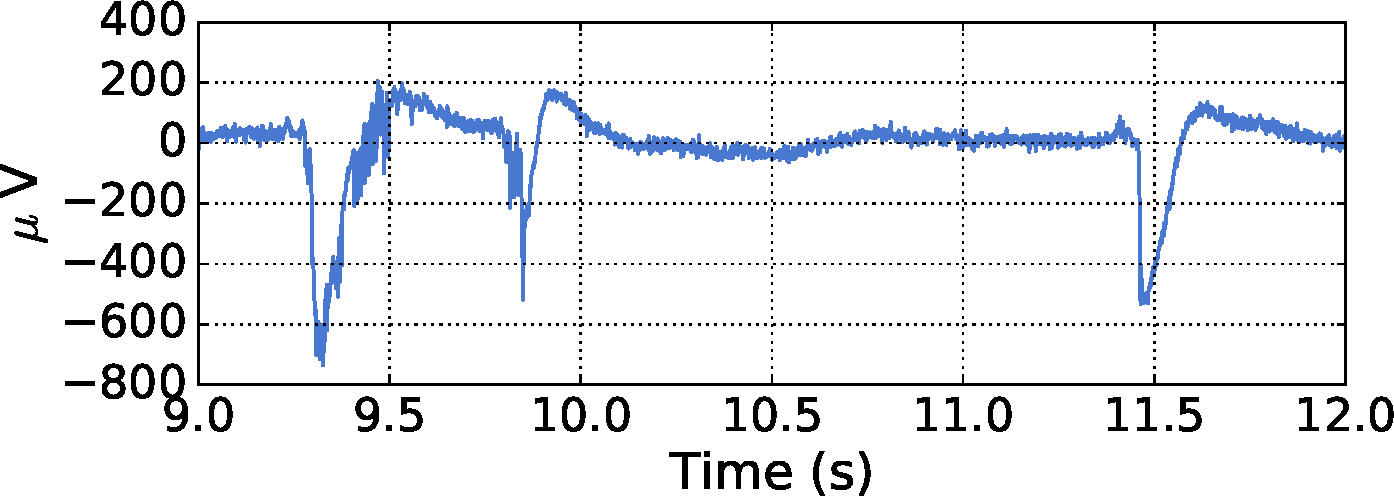
\includegraphics[height=4cm]{figures/spike_atomsa.pdf}
             \label{fig:sommaire:spikedata}} \\
             \subfigure[Estimated atoms]{
             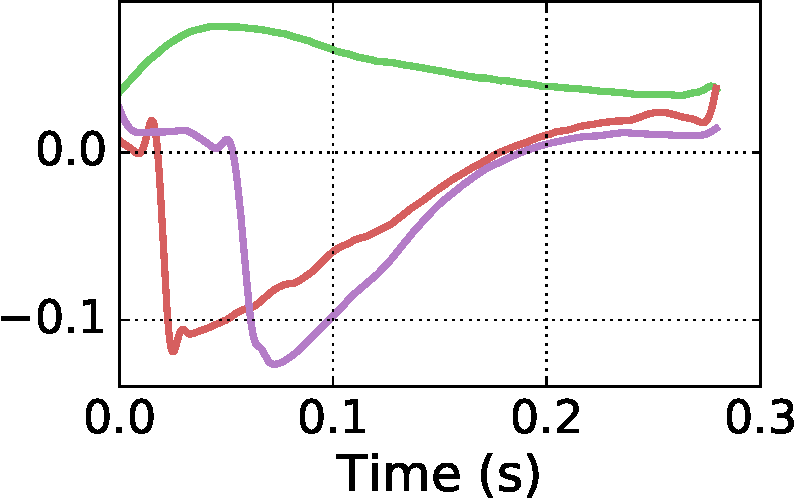
\includegraphics[height=4cm]{figures/spike_atomsb.pdf}
             \label{fig:sommaire:spikeatoms}}

            \caption[]{Atoms learnt by $\alpha$CSC on LFP data containing epileptiform spikes with $\alpha=2$.}
\end{figure}


\section*{Conclusion}

Methods research in neuroimaging is a marriage between computer science and neuroscience. It is a collaboration between two complementary disciplines -- the aim is to bring to the table computation tools which can help scientists make new discoveries. Certain aspects of this interdisciplinary subfield is of course to incrementally develop existing tools: for example, those that can help achieve a better prediction score, or a better localization accuracy in estimating neural sources. However, an orthogonal but equally important aspect of methods research is to develop tools which allow fundamentally new ways to interact with the data. This thesis is an attempt to advance this goal by developing tools for automated analysis in electrophysiology.

It has now become evident to us that in order to achieve the goal of reproducible research, large public datasets are the key and automated methods to analyze them are indispensable. While every neuroscientist's ambition is to generate new insights and push the frontiers of our knowledge of the brain, this is often not possible due to the weak effect sizes which cannot be uncovered in small datasets. When the null hypothesis cannot be rejected, it is a common practice to start fishing for significant results by testing multiple hypotheses and reporting the most favourable ones. This has resulted in a body of literature where a large fraction of the results lie on shaky grounds. 

In this thesis, we developed a new specification known as the \ac{BIDS}, which facilitates data sharing between neuroscientists by promoting common standards for storing measurement related metadata. We also provided an overview of the challenges in reproducible data analysis with respect to \ac{MEG}/\ac{EEG} data. As contributors to the MNE software package, we felt particularly well positioned to address  the software related challenges: complex pipelines, software versions, random initialization \emph{etc.,} and standardized recommendations for each stage of these pipelines. We did this by reanalyzing a group study on Faces dataset~\citep{wakeman2015multi}. To ensure reproducible results, the entire analysis was scripted and the plots generated automatically using the \code{sphinx\_gallery} package\footnote{https://sphinx-gallery.github.io}.

In order to even further push the goal of reproducibility via automation, we developed two new methods for analyzing electrophysiological data. The first method, called \emph{autoreject}, aims to streamline the removal of data segments containing artifacts which is a basic preprocessing step in almost every analysis chain. We develop an efficient method which uses a parameter search method known as Bayesian optimization. Our approach was able to facilitate re-analysis of the \ac{HCP} data for benchmarking. Our second method, known as \emph{alphacsc} enables mining neural time series for new oscillatory structures. Not only that, it is a tool to estimate more accurate waveform shapes than what is possible using traditional Fourier analysis. We demonstrated in our work that it was able to discover nested oscillations from the data.

These technologies can still be considered to be in their infancy in many respects. Just as source localization methods in \ac{MEG}/\ac{EEG} have evolved from dipole-based models to distributed methods to more sophisticated models implementing structured sparsity, these new methods are likely to undergo an evolutionary process of incremental improvements. If we consider the example of \ac{CSC}, our model based on alpha-stable distributions extended the computer vision models to be able to handle heavy-tailed distributions that is characteristic in neural data. Obviously, this is not the end of the road. Tuning hyperparameters in \ac{CSC} models is still notoriously difficult, but it is not impossible if there is an supervised task at the end of the pipeline. Multiscale dictionaries might be critical for brain signals considering that the oscillations can have varying support. As the problem is non-convex, smarter initialization strategies such as those based on \ac{MCMC} could lead to more accurate estimates~\citep{bachem2016fast}. It will also soon be necessary to build streaming \ac{CSC} algorithms based on stochastic approximations to deal with larger datasets.

Unlike computer vision or natural language processing, high-risk industries such as healthcare require transparent algorithms. It is no longer sufficient to be able to merely achieve higher prediction accuracy.
% In fact, a large fraction of neuroimaging data, even that which is available publicly, is unlabeled or at best weakly labeled.
In our work on \emph{autoreject} and \emph{alphacsc}, we leverage such public data to develop algorithms which are easy to interpret and diagnose. \emph{Autoreject} identifies the data segments to be removed based on a single parameter which is easy to understand and is automatically tuned. In the same way, \emph{alphacsc} mines the prototypical waveforms directly so as to replace indirect measures for unearthing phenomena of interest.

In this thesis, I outlined a strategy for reproducible research in the future: public datasets with large sample sizes and automation. However, the focus of some of my work was limited to automation on the scale of single subjects. Even though this does enable us to analyse large datasets, it can be sometimes limiting as it does not allow us to pool data across subjects so as to discover more subtle effects. As we enter an era of fast-paced science, such data-driven tools will become indispensable. While a lot of methods research has been focussed on improving the signal-to-noise ratio in each dataset, this may turn out to be not as important when dealing with larger datasets. Looking ahead, we will increasingly prefer large datasets which are not perfectly denoised rather than a smaller perfectly denoised dataset. New tools will need to be developed in order to enable clinicians to rapidly probe the brain so as to identify signals and structures of interest, quantify uncertainties along with the accuracy scores, perform quality control, and interactively visualize their data.


\clearpage
% Group study
\chapter{Introduction}
\label{chapter:intro}
\pagestyle{mainmatter}
\pagenumbering{arabic}

\epigraph{\small\itshape ``Progress in science depends on new techniques, new discoveries and new ideas, probably in that order.''}{\small\textit{---Sidney Brenner}}

\begin{figure}[ht!]
\centering
\begingroup
\etocstandardlines
%\renewcommand{\etocbkgcolorcmd}{\color{lightgray}}
\renewcommand{\etocbelowtocskip}{0pt\relax}
\fboxsep1ex
\etocframedstyle [1]{\fbox{\makebox[.4\linewidth]{\etocfontminusone
Contents}}}
\localtableofcontents
\endgroup
\end{figure}

\clearpage

Understanding the human brain is one of the most significant challenges of the 21st century. The human brain is arguably the most complex  organs of the human body, which performs a wide range of cognitive functions: from visual recognition to language understanding, speech, social interaction, and executive control. Pathologies of the brain are perhaps on of the biggest challenges for western medicine today. Medical interventions and drugs for major infectious diseases are available today, and individuals can expect to live up to the mid 80s and even into their 90s. Yet, we still do not have a good grasp over most mental pathologies: Parkinson's, Alzheimer's, dementia, epilepsy to name a few. This is despite the fact that someone today who lives into their mid 80s has a 50\% chance of contracting Alzheimer's~\citep{alzheimer20162016}.

Our current understanding of the brain is a result of decades of concerted efforts across multiple disciplines ranging from molecular biology, genetics, physiology, cognitive and behavioral neuroscience, to statistics, computer science, and data science. A relatively new subfield here is brain imaging, also known as neuroimaging. Brain imaging refer to a set of technologies where a snapshot of the brain is taken to measure either the anatomy or various aspects of function. The grand vision is to be deploy them in hospitals to help diagnosis, in surgeries, in \acp{BCI}, or in research for neuroscientists to better understand the brain. 
In this thesis, we will focus our attention on measuring the electric currents and/or corresponding magnetic field from the brain, using electroencephalography, magnetoencephalography, and local field potentials. 
These methods have the property of possessing a high temporal resolution, which is particularly useful for extracting the temporal dynamics of brain signals.

In the following sections, I will describe the context surrounding the thesis. After a brief introduction to the field of electrophysiology, I will delve into how the field has been shaped in recent years by the reproducibility crisis, and how data sharing is going to help alleviate this problem to a large extent. However, the rise of data sharing and large sample sizes makes it difficult to still rely on manual data analysis which does not scale and is not reproducible. To cope with this challenge, we must start relying on automated and data-driven methods for discovering new effects. To this effect, I will introduce two new algorithms \emph{autoreject} and \emph{alphacsc}. This is followed by a refresher on background material that might be useful to refer to when reading the thesis. The chapter ends with the contributions of this thesis and the list of papers published during the PhD.
 
%\section{Modern brain imaging}
%Brain imaging tools today can be placed along three axes: their temporal resolution, their spatial resolution, and the level to which they are invasive.

\section{Electrophysiology}

\begin{figure}[htb]
\begin{center}
   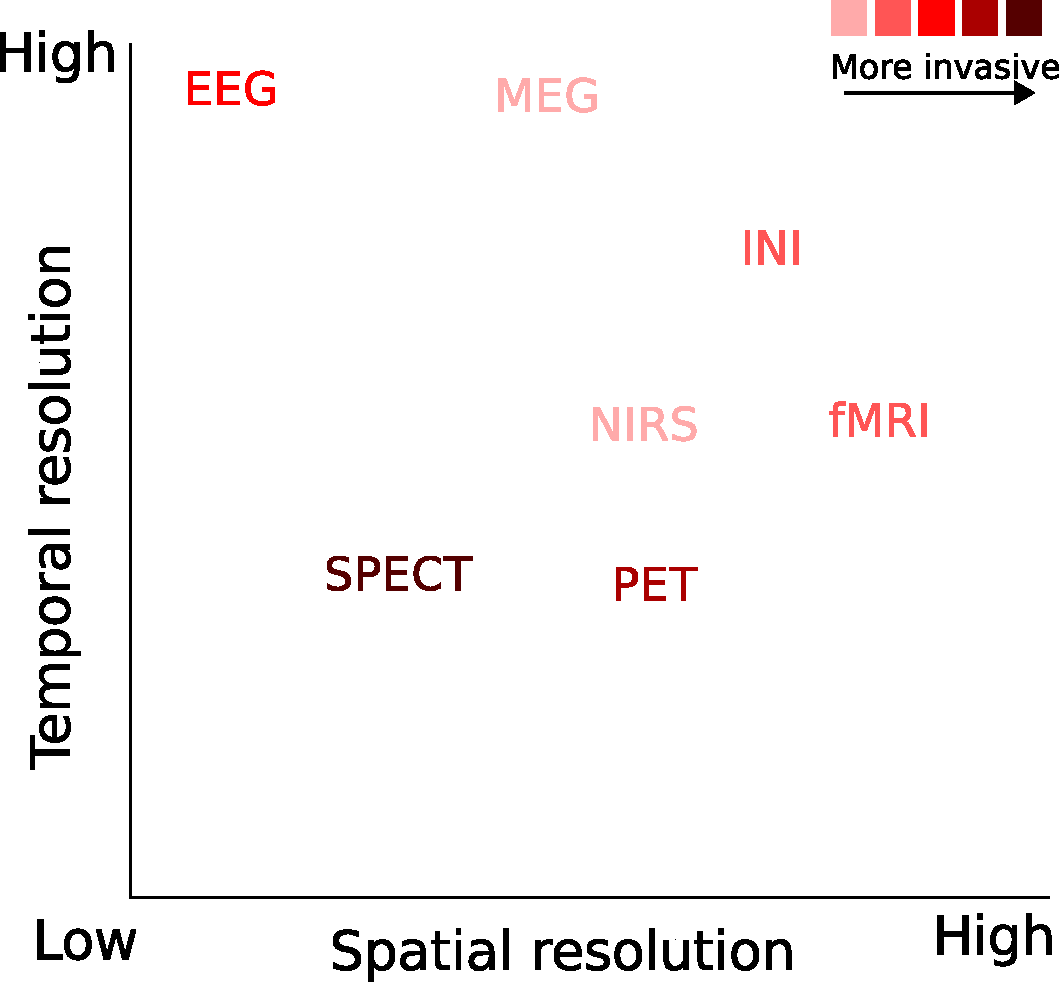
\includegraphics[width=0.5\linewidth]{figures/neuroimaging_methods.pdf}
\end{center}
   \caption[Various neuroimaging methods differ in terms of the information they measure.]{Various neuroimaging methods differ in terms of the information they measure. MEG=magnetoencephalography, EEG=electroencephalography, NIRS=near-infrared spectroscopy, PET=positron emission tomography, SPECT=single photon emission tomography, and INI=Inverse imaging, a method to speed up acquisition of fMRI images, ECoG=Electrocorticography, LFP=Local Field Potential.}
   \label{fig:neuroimaging_methods}
\end{figure}

The study of electrical properties of the biological cells and tissues is known as electrophysiology. Biological tissues have electrical properties due to the presence of ions. Just as we can measure voltages in electrical appliances, it is possible also to measure these voltages on living tissues. These modalities have the advantage of directly measuring the brain activity, as opposed to an indirect measure, which is for example the case in \ac{fMRI}.
Brain imaging techniques are characterized by their temporal and spatial resolution, \textit{i.e.,} the time scale at which it can measure brain activity, and also the accuracy of localizing the source of the activity. Figure~\ref{fig:neuroimaging_methods} summarizes different neuroimaging methods with respect to their temporal and spatial resolution. In the case of \ac{fMRI}, as it measures the blood flow which is a response to neural activity and slowly changing, its temporal resolution cannot be high. 

There are a number of modalities to measure the electrical potentials in the human body, the most well-known being perhaps \ac{ECG} which is used to measure the heart beats. However, in our work, we will focus on only three which are relevant for studying the brain. Each of these methods produces a multivariate time series.

\paragraph{Electroencephalography: } \Ac{EEG} is a portable and non-invasive measurement modality that is frequently used in the context of \acp{BCI}. In electroencephalography, an array of electrodes on an \ac{EEG} cap are placed on the scalp to measure the voltages with respect to a reference electrode. The voltage it measure is not the result of a single neuron but instead a summed potential of populations of thousands of neurons. It has a high temporal resolution (in the order of \emph{ms}), however the spatial resolution is not so high as the skull smears the signal.

\paragraph{Magnetoencephalography: } Any electric current is associated with magnetic fields as a consequence of Maxwell's theory. 
Therefore, the brain generates tiny magnetic fields which  wrap around the currents according to Maxwell's right hand thumb rule. The flux is tiny ($\sim10^{-12}T$) compared to the earth's magnetic field ($\sim10^{-4}T$), and to measure this one would need very sensitive electronics and heavy noise cancellation. The measurement itself is done done in a shielded magnetic room made of three layers of metals. The sensors are superconducting coils which capture the magnetic flux. They are immersed in liquid helium cooled to very low temperatures, so as to lower any loss in signal due to resistance. A typical device contains two types of sensors: gradiometers and magnetometers. While the magnetometer measures the absolute magnitude of magnetic field, the gradiometer measures derivative of the field. \Ac{MEG} has the advantage that the skull does not deteriorate the signal quality as in \ac{EEG}.

\paragraph{\Ac{LFP}}
The Local Field Potential is an invasive method that measures the electrical potential in the extracellular space of the brain tissue. In contrast to \ac{EEG}, \ac{LFP} are recorded in depth, from within the cortical tissue and can therefore measure more localized populations of neurons.

\section{Context of the thesis}
This emerges out of the recent movements in reproducibility and data sharing in neuroimaging. It focuses on simplifying data analysis through better educational tools and automated methods to enable reproducible analysis in the age of big data.

\subsection{The reproducibility crisis}
\label{sec:reproducibility_crisis}
Even though thousands of papers are published every year about different aspects of the brain, our understanding of this complex organ has not scaled in proportion. A large part of the reason has been attributed to what is known as the reproducibility crisis~\citep{ioannidis2005most, simmons2011false, button2013power}. %Replication is closely related to the concept of reproducibility which refers to the idea that an experiment produces the same result when performed again under the same conditions. Replication is a stronger condition as it requires similar results or identical conclusion even if there are some minor variations in the experimental procedures. 
Progress in science rests on reproducible experiments. Reproducibility refers to the fact that the findings of an experiment can be regenerated independently if the code, data, and related software was provided. In many fields, however, a large fraction of experiments cannot be reproduced. In psychology, for instance, it was estimated that over half of the papers were not reproducible~\citep{open2015estimating}, and even those which could be reproduced tended to have a weaker effect size compared to the original studies. 

The reasons for unreproducible results can be many~\citep{baker20161}, some being: 1) confirmation bias, the tendency to selectively report only experiments that conform to the researcher's pre-existing beliefs, 2) ``p-hacking''~\citep{simmons2011false}, or the tendency to try multiple hypothesis to get a positive result, 3) publication bias or the absence of incentives to publish negative results~\citep{rosenthal1979file}, and 4) pressure to publish. There are now an accepted set of recommendations to counter many of these issues: 1) pre-registering research plans to avoid confirmation bias and even report negative results, 2) correct for multiple comparisons, the most conservative method being the Bonferroni correction~\citep{dunn1961multiple}. 

Brain imaging has its own set of issues which can be linked to reproducibility crisis: 

% vul2009puzzlingly
% yendiki2014spurious

\begin{itemize}[noitemsep,partopsep=0pt]
\item \textbf{Power failure:} This is arguably one of the central issues in the reproducibility crisis today and has received by far the most attention. The statistical power of a study refers to the likelihood of discovering an effect of interest, given the sample size. Small sample sizes translate into underpowered studies which means that the chance of a false discovery is high. In order to discover the effect of interest, the study must be appropriately powered.
\item \textbf{Multiple comparison:} This is essentially a manifestation of ``p hacking'' that is a result of of the large number of voxels or time points in neuroimaging. For instance, in the famous dead salmon study~\citep{bennett2009neural}, a significant effect was found even if none was expected simply because the hypothesis testing (comparisons) was done over each voxel.
\item \textbf{Differences in software versions:} Changing software versions can lead to different results. For instance in the case of Freesurfer software, differences in volume were found in the range of $8.8\% \pm 6.6\%$~\citep{gronenschild2012effects}.
\item \textbf{Complex pipelines:} Neuroimaging pipelines involve a number of choices at each processing stage, and there is currently no consensus on how to choose the right pipeline. Often, these methodological choices are not even documented. It is estimated that there are almost as many unique pipelines as there are studies~\citep{Carp2012289}.
\item \textbf{Confounds:} There are several methodological confounds such as head movements~\citep{yendiki2014spurious}, anatomy differences, and changes in breathing rate and depth, which can lead to spurious correlations.
\end{itemize}

In Chapter~\ref{chapter:group_study} of the thesis, we will provide concrete guidelines on how to build processing pipelines for \ac{MEG}/\ac{EEG} data. Our contribution will touch upon the issue of complex pipelines, multiple comparison, and differences in software versions in the context of \ac{MEG}/\ac{EEG}. The issue of power failure can be alleviated through data sharing as I will discuss in the next section.

\subsection{Data sharing}
\label{sec:intro_datasharing}
Power failure is essentially a consequence of small datasets. In today's collaborative and data-driven scientific environment, data sharing is useful not only from the perspective of reproducibility but also to build datasets with large sample sizes. With large datasets, it would be possible to tease apart even subtle effects~\citep{smith2017statistical} that were not possible with smaller datasets. Data sharing is beneficial not just from the perspective of replication but also from an economic perspective. Rather than collect new data for every new hypothesis, researchers can now reuse known data for answering their hypotheses.

The benefits of data sharing can be traced back to Newton and his theory of gravitation~\citep{pointofview2013}. Before Newton had developed his theory, another English astronomer, John Flamsteed had been appointed by the king to observe the stars and produce accurate charts for navigation in the seas. Over a period of 40 years, Flamsteed created a detailed catalogue that tripled the number of entries in the previously used sky atlas. When the great comet of 1680 appeared in the sky twice in close succession, Flamsteed used his data to postulate that it was not two comets but in fact the same comet which first went towards the sun and then turned away from it. Newton initially opposed this theory, but later changed his mind as he gained access to Flamsteed's unpublished catalogue. The comet had indeed turned out to be an important benchmark for Newton's theory of gravitation.

It is hard to imagine in this day and age that a theory as fundamental as the laws of gravitation could have been data driven. Data sharing is fundamental not only to reproducible science, but also it forms the cornerstone for learning stronger models and benchmarking new algorithms. Consequently, in machine learning, recent breakthroughs have been powered by the increase in data sharing and computation. This includes the recent resurgence of deep learning~\citep{deng2009imagenet}, Q learning~\citep{watkins1992q, bellemare2013arcade}, natural language processing for language translation~\citep{halevy2009unreasonable}, speech recognition~\citep{paul1992design}, and even the mixture of experts model~\citep{jacobs1991adaptive} for IBM Watson~\citep{ferrucci2010building}. The maxim, ``more data beats a cleverer algorithm''~\citep{domingos2012few} has held up remarkably well across disciplines and over the ages.

Of course, neuroscientists are beginning to realize the importance of sharing data. In recent times, neural data has started being shared through international consortiums~\citep{van2013wu, ollier2005uk} and data repositories~\citep{poldrack2013toward, gorgolewski2015neurovault}. While in the case of Newton, he gained access to the catalogue without permission, today it is possible to publish dataset papers in targeted journals so as to assign the credit where it is due. Yet, there is an unaddressed gap in terms of the ideal of data sharing and the practice of data sharing. Neuroimaging experiments are often very complicated, and it is not enough to share simply the data, but also the metadata and information regarding the experimental protocols in a well-structured format. 
In the absence of this information, shared data is not \emph{reusable} in the same way that uncommented and ``spaghetti code'' (poorly structured and complicated programs) is not useful even if shared publicly. There isn't an accepted consensus in the community on the practices of sharing data and there is a need to establish a standard. 
In Chapter~\ref{chapter:group_study}, we will present a new standard known as the \ac{BIDS}, which is intended to address this gap. 
It is a collaborative effort between software developers and neuroscientists across various laboratories to establish a consensus on the standards and build tools to facilitate adoption of the standard.

\subsection{Automation}
\label{sec:automation}

Back in 2014, Nature published a bold article~\citep{hayden2014automated} which described a vision for the future of science: ``solving the problem of bringing McDonald's-like efficiency to scientists''. This would in turn lead to cheaper, more efficient and reliable research. While it goes on to describe many biology labs which are automating experiments, the benefits of automation in the neuroimaging community are yet to be widely recognized. Automation not only saves time but also makes the research more reproducible, as was noted in a recent guide to improve the transparency and reproducibility of neuroimaging research~\citep{gorgolewski2016practical}. The authors point out that manual work may seem easy at first, if the analysis has to be performed only once. However, this is not always the case as ``quite often in the course of a project, parameters are modified, subjects are changed, and processing steps need to be rerun. This is a situation in which having a set of scripts that can perform all of the processing steps automatically instead of relying on manual interventions can really pay off.'' As large datasets become more common in neuroimaging, automation will indeed become a necessity rather than a luxury.

In neuroimaging, there are in fact several avenues for automation:
\begin{itemize}[noitemsep,nolistsep,nosep]
\item \textbf{Reducing interactivity:} While interactive graphical user interfaces are excellent tools for browsing the data, they fall short when it comes to scaling the analysis, which is necessary for a sufficiently powered study. 

\item \textbf{Parameter tuning:} Most algorithms, although scripted, still require hyperparameters to be tuned. These hyperparameters could be the number of ICA components to choose or the regularization parameters, and can vary for each subject.
%This could be the number of trials to perform in an experiment, the number of components to select in a \ac{PCA} decomposition, or the regularization parameter in inverse solvers.
\item \textbf{Annotation and labeling:} A large fraction of neuroimaging data that is available is unlabeled or at best weakly labeled. This is because expert annotations are expensive, and cannot be crowdsourced. Automated tools based on unsupervised learning can play a major role in this regard.
\item \textbf{Quality control:} Currently, quality control is performed manually by inspecting the data to spot outliers. While data inspection cannot be overlooked, it can be performed more efficiently through automated documentation of data analysis and log reports such as the Jupyter notebook and the MNE web report~\citep{dengemann2015conc}. At the same time, advanced statistical trend analyses as in the Automated Statistician project~\citep{duvenaud2013structure} can be used for creating summaries.
\end{itemize}

There have been some steps taken in this direction, most notably the Neurosynth platform~\citep{yarkoni2011large} which facilitates large-scale meta analysis to integrate activations maps across studies using machine learning. On the software side, the Freesurfer software package~\citep{dale-fischl-etal:99, fischl-serena-etal:99} provides a \code{recon-all} command that performs cortical segmentation automatically without any human intervention. In MNE, this philosophy is now being adopted starting with automated covariance estimation~\citep{engemann2015automated_new}.

In this thesis, we will consider an algorithm that automatically annotates artifacts in the data~\citep{jas2016automated, jas2017autoreject}. This is a first step that any \ac{MEG}/\ac{EEG} processing pipeline has to go through but it is often done manually. A reason for this is that existing algorithms are not designed to be \emph{transparent}. Since for most scientists, the key to new insights is an artifact-free dataset, they would rather spend extra effort in doing this manually rather than depend on a generic algorithm which is difficult to interpret. %However, this is problematic as it can lead to a selection bias: they might end up rejecting data segments which helps them confirm their hypothesis. 
Merely based on anecdotal reports, this process can take up to a week even for a moderately sized study of 10--20 subjects.

This is what led us to propose \emph{autoreject}, which we describe in Chapter~\ref{chapter:autoreject}. It is an algorithm which can be used to mark bad segments of the data. The key insight is that, often certain sensors in the device are intermittently corrupted rather than continuously. We validate our algorithm against 3 benchmarks on the \ac{HCP} dataset~\citep{larson2013adding} which is manually annotated with bad segments. In the process, our work also represents one of the first attempts at reanalyzing the MEG component of the HCP dataset.

\subsection{Representation learning for data-driven discovery}
\label{sec:representation_learning}
In the last 100 years since the invention of \ac{EEG}, scientists have discovered several different brain oscillation patterns such as alpha waves, K-complexes, and mu rhythms. The oscillations and interactions between them have served as biomarkers for different brain functions and pathologies. Alpha waves have been implicated in attention, K-complexes in sleep, and mu rhythm in motor activity. 

Considering the complexity of the human brain, clearly these waveforms represent only a fraction of the cognitive functions that the brain may perform. As a result of the wealth of data now available through the data sharing movement described in Section~\ref{sec:intro_datasharing}, the future neuroscientist will be able to mine such waveforms from large datasets. Imagine if neuroscientists had at their disposal a tool similar to Google Photos\footnote{\url{https://photos.google.com/}}. In the same way that Google Photos can automatically find faces and group photos, such tools will be able to find prototypical oscillations and cluster the data using them. Clicking on any of these waveforms would retrieve the data associated with them.

\begin{figure}[htb]
\begin{center}
   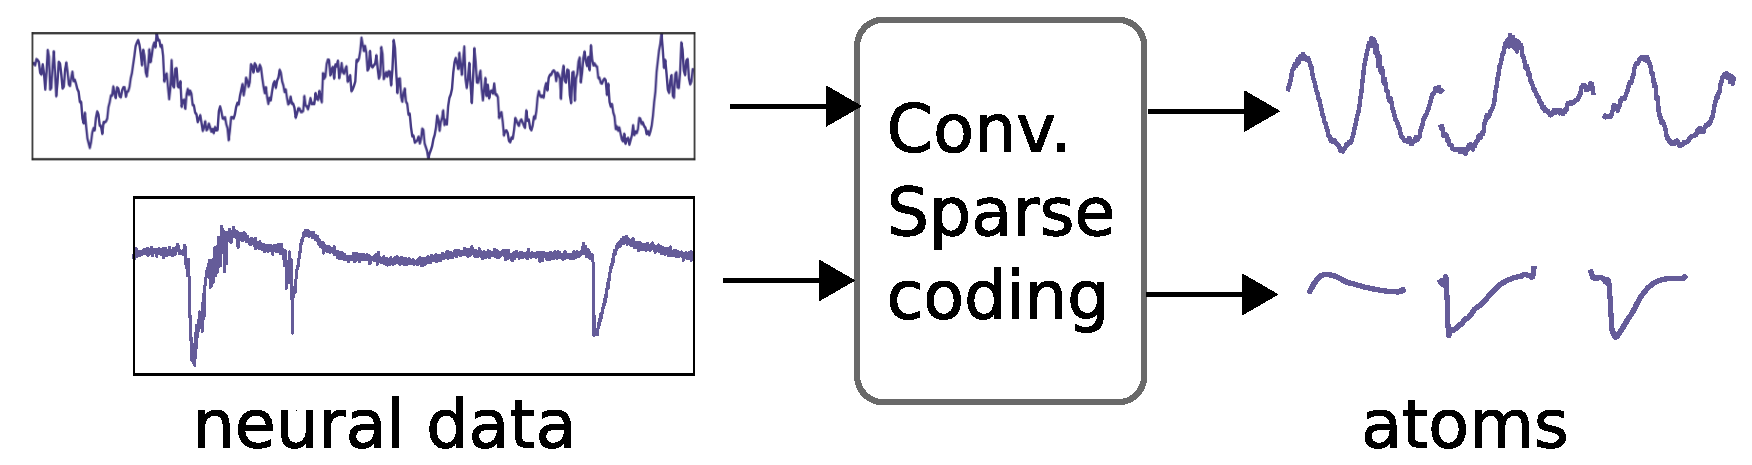
\includegraphics[width=0.7\linewidth]{figures/schema.pdf}
\end{center}
   \caption[Convolutional sparse coding]{An illustration of how Convolutional sparse coding can be used to automatically mine prototypical waveforms}
   \label{fig:neuroimaging_methods}
\end{figure}

However, photos are inherently different from neural data. First, neural data can be buried in noise and corrupted by high amplitude artifacts. Second, images are labelled owing to crowdsourced data as in the case of  Imagenet~\citep{deng2009imagenet}, but neural data is not. 
Expert annotations in the case of neural data are not easily available.
Finally, it is spatiotemporal data with different dynamics than the 3D world that photos capture. This is where \ac{CSC} can play a role by extracting prototypical features from the data. It is an unsupervised algorithm from computer vision, which can learn shift-invariant dictionaries of prototypical waveforms (atoms) from the data using the convolution operations. For a more comprehensive background on \ac{CSC}, the reader may read Section~\ref{sec:background_dict_learning} later in this chapter.

\ac{CSC} algorithms do not approximate the signal using Fourier (or sinusoidal) basis. While this is the conventional technique for extracting signals buried in noise, the approximation can degrade the shape of the signal, which can be a biomarker in many clinical diseases~\citep{cole2017brain}. As an example, a square wave would need an infinite series of sinusoids for a good approximation. Of course, transients can be better approximated using wavelets but it is clearly not sufficient for other shapes of data. Rather than fix the basis to be Fourier or wavelet, the \ac{CSC} approach is to learn \emph{both} the basis and the coefficients.

In our work presented in Chapter~\ref{chapter:alphacsc}, we extend conventional \ac{CSC} algorithms for heavy-tailed noise. We reformulate the optimization problem as a \ac{MAP} inference with an alpha-stable distribution to replace the reconstruction loss. Our results show that this kind of algorithm is robust to the presence of artifacts and can be used to uncover temporal structures from neural signals, even those involving nested oscillations.


\section{Background}

Here, we will introduce some basic linear algebra, optimization, and machine learning concepts that will be useful particularly in Chapters~\ref{chapter:autoreject} and \ref{chapter:alphacsc} on \emph{autoreject} and \emph{alphacsc}.

\subsection{Norms}
Informally speaking, a norm is used to measure the length or size of a vector. It must also satisfy some properties, but it will not be of concern for us in this thesis. It is sufficient to know the mathematical expression, how it behaves, and the physical property that it captures.
\theoremstyle{definition}
\newtheorem{definition}{Definition}[chapter]
%
%
\vspace{\parskip}
\begin{definition}{($\ell_p$ norm.)}
For $1 \leq p < \infty$, the $\ell_p$ norm of a vector $x$ is defined by:
\begin{equation}
\|x\|_p = \Big(\sum_n \ \lvert x_n \rvert^p \Big)^{1/p}
\end{equation}
\end{definition}
%
%
\vspace{\parskip}
\begin{definition}{($\ell_\infty$ norm.)}
The $\ell_\infty$ norm of a vector $x$ is defined by:
\begin{equation}
\|x\|_{\infty} = \sup_n \ \lvert x_n \rvert
\end{equation}
\label{def:norm}
\end{definition}
As we are taking the supremum, this norm is sensitive to large values in the vector, which is needed for measuring artifacts.
%
%
\vspace{\parskip}
\begin{definition}{(Frobenius norm.)}
The Frobenius norm of a real-valued matrix $A$ is defined by:
\begin{equation}
\|A\|_{\mathrm{Fro}} = \| \mathrm{vec}(A) \|_2 = \sqrt{\mathrm{trace}(AA^\top)}
\end{equation}
%
The Frobenius norm is a matrix norm that is simply the $\ell_2$ vector norm of the vectorized matrix $\mathrm{vec}(A)$.

\end{definition}

\subsection{Cross validation}

Cross validation is a statistical technique to estimate how well a predictive model will \emph{generalize} to unseen data. We will be using cross validation in our \emph{autoreject} work presented in Chapter~\ref{chapter:autoreject}. Cross validation is normally performed by partitioning the data into two and learning the model from one part (typically the larger one) while validating it on the other. These two parts are known as the \emph{training} and the \emph{validation} sets respectively. In order to get reliable estimates of the model performance, this procedure is repeated multiple times and the results are averaged.

Depending on the data, different types of partitioning schemes are preferred. In \emph{K-fold} cross validation, the data is divided into $K$ equal parts (with or without shuffling the samples), where $K - 1$ parts are used for training and the $K$th part is used for validation. In a \emph{stratified} cross-validation scheme, the partitions are done such that each partition has roughly equal number of samples from each class.

\paragraph{Grid search: } When cross validation is used for selecting the best model by exhaustively searching over all possible parameters that the model can admit, it is known as grid search.

\paragraph{Random search: } Sometimes grid search is too slow, and it is better to try parameters sampled randomly without a considerable loss in performance. This is known as random search.

\paragraph{Nested cross validation: } When cross validation has been used for finding the best model, a separate unseen partition, known as the \emph{test} set, is needed to assess the generalization power of the best model. The test set must be different from all the data that was seen so far, including \emph{both} the training and the validation sets. This is done to avoid a circularity bias as noted in \cite{varoquaux2017assessing}. Therefore a nested cross-validation scheme is necessary where in each outer loop, the best model is found, and its performance is computed.

\subsection{Bayesian optimization}


\begin{figure}[htb]
\begin{center}
   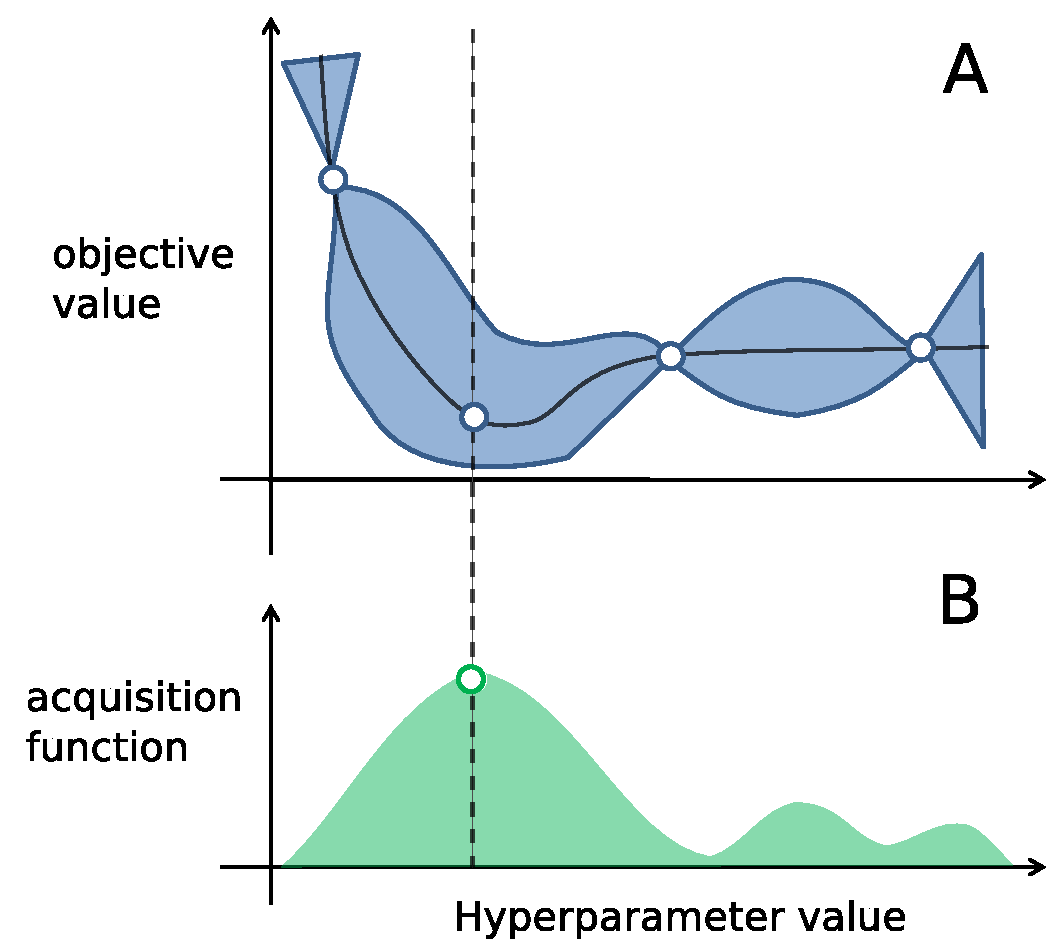
\includegraphics[width=0.7\linewidth]{figures/bayes_opt.pdf}
\end{center}
   \caption[Bayesian optimization for parameter tuning]{An illustration of how Bayesian optimization works by combining (A) Gaussian process to estimate uncertainties on the objective function for the parameter space, and (B) Acquisition function to balance the ``exploration'' \emph{vs} ``exploitation'' dilemma.}
   \label{fig:bayes_opt}
\end{figure}

Sometimes grid search is too slow and random search is not as accurate for tuning hyperparameters. In such cases, one may have to rely on more efficient black box optimization techniques. Bayesian optimization~\citep{snoek2012practical} is one such method which is a sequential method, and iteratively improves the objective function that we are optimizing.

Since these method must work for any kind of function which is unknown and may not be necessarily convex, we cannot rely on classical gradient based methods. The central idea in these types of methods is to search as much of the parameter space as possible, while keeping a record of the objective values evaluated so far. A very natural strategy is therefore to either search around points which have high objective values, or in those areas where it is unknown. This is indeed a case for the classic  ``exploration'' \emph{vs.} ``exploitation'' dilemma that is well-known in computer science.

In order solve this dilemma, an \emph{acquisition function} is typically used. While the ``exploitation'' component of this function is easy to compute from the objective values, in order to compute the ``exploration'' component, we can fall back upon \acp{GP}~\citep{rasmussen2004gaussian}. Given the points evaluated until now, a \ac{GP} can be used to estimate the uncertainty in the rest of the search space. 


\subsection{Dictionary learning}
\label{sec:background_dict_learning}

\paragraph{Sparse Coding:} A \emph{dictionary} is a set of \emph{atoms} (also known as filters sometimes) which can be combined with certain \emph{coefficients} (or activations) to approximate the data. 
The atoms could be fixed (for example wavelets or Gabor), or they could be learned directly from the data itself. As such, there is no requirement of orthogonality on the atoms. 
To learn a representation of the data boils down to estimating the coefficients used in the approximation, which are often assumed to be sparse, \emph{i.e.}, they have very few non-zero values. 
The learning algorithm is therefore called \emph{sparse coding} and the coefficients learned are known as the \emph{sparse code}.

Sparsity can be promoted by using an $\ell_0$ or $\ell_1$ penalty, which helps maintain a compact representation. Note that the $\ell_0$ ``norm'' simply counts the number of elements in the vector (c.f., Definition~\ref{def:norm}) , therefore adding it as a regularizer will favour solutions that have fewer non-zero elements. In the traditional approach, it is quite common to start off with an \emph{overcomplete} dictionary, \emph{i.e.,} to have more atoms than would be needed, and only estimate the coefficients (keeping the atoms fixed). This can be done, for example, using matching pursuit~\citep{mallat1993matching}, which is a greedy algorithm for sparse approximations.

\paragraph{Learning atoms:} It is easy to see that the overcomplete approach is memory intensive as it has more atoms that necessary, but also this approach requires making assumptions about the shape of the atoms in the dictionary. Nowadays, it is more common to learn the atoms in addition to the sparse code, which is known as \emph{dictionary learning}. Dictionary learning can be thought of as a data decomposition method (or matrix factorization) technique (like \ac{PCA} or \ac{ICA}), but with a sparse regularization. Typically, the convex relaxation of the $\ell_0$ penalty, the $\ell_1$ penalty is used in these situations. The problem is biconvex after the relaxation, and can therefore be solved by alternate minimization. Dictionary learning is now being used for denoising~\citep{elad2006image}, inpainting~\citep{mairal2009online}, and classification~\citep{mairal2009supervised}. 

\paragraph{Coding for shift invariance:}
In traditional dictionary learning, the signal or the image is divided into patches and these patches are used as samples for the learning. The main disadvantage of this method is that it results in redundant atoms that are shifted versions of each other. This is the reason a shift-invariant version of dictionary learning is needed. One of the earliest paper in this regard can be credited to \cite{lewicki1999coding}. In their work, the dictionary was fixed and the shift-invariance was encoded using convolutions. 
This is possible because the convolution operator is defined by an integration (correspondingly summation in the discrete domain) as below.
\vspace{\parskip}
%
\begin{definition}{(Convolution)}
\label{def:convolution}
A convolution of two functions $f$ and $g$ is written $f * g$ and computed as:
\begin{equation}
(f * g)(t) \triangleq \int_{-\infty}^{\infty} f(\tau)g(t-\tau) d\tau
\end{equation}
\end{definition}

In the discrete case where $f$ and $g$ are vectors with finite support $[0..M]$ and $[0..N]$ and $N > M$, this can be rewritten as:
%
\begin{equation}
(f * g)[n] = \sum_{m=0}^{M-1} f[m]g[n-m]
\end{equation}
%
so that $f * g$ has a support of $[0..(N - M + 1)]$ if the edges are truncated. As we can see, if either $f$ or $g$ is zero padded, the other function can be shifted along these zeros yielding the same result.

As a result of the convolutional approach, the atoms learned are not redundant and the location of the atom is encoded in the activations. This type of approach is refered to as \ac{CSC} or shift-invariant dictionary learning in the literature. In practice, an overcomplete dictionary in the shape of a Toeplitz matrix is constructed by shifting the atoms across time. This is the same formulation which is still being used to code shift invariance even if the learning algorithms are more sophisticated now. More recent work by \cite{grosse2012shift} have made use of the Fourier transform to solve the problem in Frequency domain and compute an inverse transform of the learned dictionary in the end. Another approach that has proved to be quite efficient is the so-called predictive sparse coding which uses neural networks~\citep{kavukcuoglu2010learning}. It is hard to summarize all the work in this area, but it suffices to say that shift-invariant dictionary learning has been gaining popularity in audio signals, images, music, and now for neural data (See Section~\ref{sec:alphacsc_intro} for a more comprehensive list of references).

\subsection{Iterative solvers for convex problems}

In our \emph{alphacsc} work presented in Chapter~\ref{chapter:alphacsc}, we will be using a number of convex optimization methods. Let us first recall what is a convex function before diving into the details of these methods.
\vspace{\parskip}
\begin{definition}{(Convex function)}
A function $f$ is convex if it satisfies
\begin{equation}
\forall x_1, x_2 \in X, \forall t \in [0, 1]: f(tx_1 + (1 - t)x_2) \leq tf(x_1) + (1 - t)f(x_2)
\end{equation}
\end{definition}

In other words, for any two points on the function, the line joining those two points lies above the graph of the function. A convex function lends itself to the property that the global minimum is also necessarily the local minimum. This concept can also be extended to define strong convexity which guarantees that the local minima is not only the global minima, but also it is unique.

We will be solving unconstrained minimization problems of the form:
\begin{equation}
x^{\star} = \argmin_x \|Ax - b\|_{2}^2 + \Omega(x)
\end{equation}
\label{eq:linreg_minimize}
%
where typically $A \in \mathbb{R}^{n \times p}$ is the design matrix with $n$ rows (samples) and $p$ columns (features), $x \in \mathbb{R}^p$, and $b \in \mathbb{R}^n$. A penalty or regularization term $\Omega(x)$ is added to prevent solutions that overfit. 
If there was no regularization term $\Omega(x)$, we could solve this in closed form and get $x^{\star} = {(A^{\top}A)}^{-1}A^{\top}b$. However, this can be computationally prohibitive as inverting $A^{\top}A$ is $\mathcal{O}(p^3)$, and iterative methods based on gradient descent are more efficient as they require only a matrix-vector dot product. These are what we shall refer to as \emph{solvers}. More importantly, these gradient based methods can work for arbitrary functions as long as we have access to the gradient (or even its approximation).

In gradient based methods, we make updates of the  form:
%
\begin{equation}
x_{k + 1} = x_{k} + \rho_k d_k,
\end{equation}
\label{eq:update_term}
%
where $\rho_k$ is the step size and $d_k$ is the search direction.

\paragraph{Gradient descent: } In the case of gradient descent, the search direction $d_k$ is the negative gradient $-g(x_k)$ and the optimal step size $\rho_k=1/L$ where $L$ is the Lipschitz constant of the gradient, which upper bounds the rate at which it changes. The intuition behind this method is that if we follow the negative gradient direction, we will progressively reach a point where the gradient is 0 and this corresponds to the minimum.

However, often the regularization term $\Omega(x)$ is not smooth, and therefore it does not have a unique derivative at all points. In these cases, we must resort to proximal gradient methods.

\paragraph{Proximal algorithms: } A common example of a non-smooth regularizer, which is encountered in practice, and will also be used in our work, is the Lasso~\citep{tibshirani1996regression}. It induces sparsity using $\Omega(x) = \lambda \|x\|_1$, where $\lambda$ controls the sparsity level. Higher the $\lambda$, the more sparse is the solution. In such situations, we can use what are known as proximal methods. The idea behind proximal methods is to take a gradient step using only the smooth part of the function, and then apply a proximal operator on the resulting iterate. 

\vspace{\parskip}
\begin{definition}{(Proximal operator)}
A proximal operator associated with a convex function $f$ is defined as:
\begin{equation}
\mathrm{prox}_f(v) = \argmin_x \bigg( f(x) + \frac{1}{2}\|x - v\|_2^2 \bigg)
\end{equation}
\end{definition}

The proximal operator can be thought of as a generalized projection operator~\citep{parikh2014proximal}. For the $\ell_1$ norm with $f(x)=\|x\|_1$, it is the soft thresholding function $\mathcal{S}_\lambda(\cdot)$ which induces sparsity, and is given by:

\begin{equation}
\mathcal{S}_{\lambda}(v) = \begin{cases}
v - \lambda \quad \text{if }  v > \lambda \\
0 \quad \hspace{22pt} \text{if } -\lambda \leq v < \lambda\\
v + \lambda \quad \text{if } v < -\lambda
\end{cases}
\end{equation}

The resulting algorithm is known as \ac{ISTA}~\citep{daubechies2004iterative, bach2012optimization}, which has a convergence rate of $\mathcal{O}(1/T)$ for $T$ iterations. Proximal algorithms are also helpful when dealing with constraints. For example, in Equation~\ref{eq:linreg_minimize}, if we had a norm-1 constraint $\|x\|_2^2 \leq 1$, this could be recast using an indicator function $i(\cdot)$:

\begin{equation}
i(x) = \begin{cases}
\infty \qquad \text{if } \|x\|_2^2 \leq 1 \\
0 \qquad \hspace{7pt}\text{if } \|x\|_2^2 > 1
\end{cases}
\end{equation}

In this case, the proximal operator can be shown to be the projection $\pi(x)$ on to the unit ball which expressed as:

\begin{equation}
\pi(x) = \frac{x}{\mathrm{max}(1, \|x\|_2)}
\end{equation} 

This is what is known as \textit{projected gradient descent}. We will encounter such constraints in our dictionary learning problem in Section~\ref{sec:m-step}. It will be used to handle the scale ambiguity between the atoms and activations when performing optimization.

\paragraph{Acceleration:} Gradient descent has slow convergence due to oscillations if the condition number of $A$ is high as it leads to pathological curvature. A faster rate of convergence can be achieved using Nesterov accelerations~\citep{nesterov1983method}, which adds a momentum term to the update in Equation~\ref{eq:update_term}.
The momentum term takes into account the update vector from the past iterations so as to dampen the oscillatory behaviour observed in classical gradient descent and \ac{ISTA}. 
This results in an algorithm known as \ac{FISTA}~\citep{beck2009fast} which has a $\mathcal{O}(1/T^2)$ rate of convergence. It has been proved theoretically that this is the fastest rate possible if we had access to only the gradient and function evaluations. The full algorithm is summarized in Algorithm~\ref{alg:fista}.

    \begin{algorithm}[H]
      \begin{algorithmic}[1] %(regularization parameter), (number of EM iterations), (number of MCMC iterations)
      \REQUIRE Regularization: $\lambda \in \real_+$, Design matrix A, b
      \STATE $x_1=0=z_1, \beta_1=1$
        \FOR{$k=1$ to $K$}
          
          \STATE $x_{k+1} = \mathcal{S}_{\lambda/L}(z_k - \frac{1}{L}g(z_k))$ \textit{\color{blue} /* Proximal step */}
          \STATE $\beta_{k+1} = (1 + \sqrt{1 + 4(\beta_k)^2})/2$
          \STATE $z_{k + 1} = x_{k + 1} + \frac{\beta_k - 1}{\beta_{k + 1}}(x_{k + 1} - x_k)$ \textit{\color{blue} /* Momentum update */}
        \ENDFOR
        \RETURN $x_{K + 1}$
        \end{algorithmic}
        \caption{Fast iterative soft thresholding algorithm}
        \label{alg:fista}
    \end{algorithm}

\paragraph{LBFGS-B}
If in the updates of Equation~\ref{eq:update_term}, instead of using the negative gradient for the search direction, we used $-d_k = H^{-1}(x_k)g(x_k)$, with $H(x_k)$ being the Hessian, it would be known as Newton's method. The Newton's method has a locally quadratic convergence, and therefore it may diverge when the current iterate is far from the optimum. Even if this is not the case, a Hessian that is not positive definite can also cause diverging behaviour. Therefore, the step size $\rho_k$ must be chosen carefully, for example using a line search strategy.

Of course, the Hessian is costly to compute and to invert, therefore quasi-Newton methods can be used which approximate it using a matrix $B_k$. Starting with $B_k = I$, we can update this matrix at each step using a cheap rank 1 or rank 2 correction. For instance, in the Broyden formula, we would do:
\begin{equation}
B_{k+1} = B_k + v.v^\top
\end{equation}
The vector-vector outer product $v.v^\top$ is the rank-1 correction in the above formula. The more advanced David-Fletcher-Powell formula uses a rank-2 correction and so does the \ac{BFGS} algorithm. When the entire Hessian matrix cannot be stored in memory, a limited memory version of BFGS~\citep{wright1999numerical} can be used where only a few vectors $v$ from the last few iterations are stored for the approximation.

\paragraph{Coordinate descent:}
In coordinate descent, we would simply minimize one coordinate at a time. The idea behind coordinate descent is rather simple, yet it performs surprisingly well in practice. Thus  Equation~\ref{eq:update_term} would be coordinatewise, \textit{i.e.,} for each iteration, we would choose a coordinate $i_k$ and perform an update:

\begin{equation}
\begin{cases}
x^{(i)}_{k+1} = x^{(i)}_{k} - \rho^{(i)}_k g^{(i)}(x_k) \quad \text{if } i=i_{k+1}\\
x^{(i)}_{k+1} = x^{(i)}_{k} \hspace{80pt} \text{if } i \neq i_{k+1}
\end{cases}
\end{equation}

Of course, we could have also solved each coordinate in closed form instead of doing gradient descent. However, in this formulation, if the non-smooth part of the objective (typically the regularizer) is \emph{separable} (\textit{i.e.,} $f(x) = \sum_i f^{(i)}(x_i)$), then it can even be extended to proximal coordinate descent. 
While coordinate descent requires $p$ times as many iterations than gradient descent, the per iteration cost is in fact much lower. Note that we do not need to necessarily solve the gradient descent completely at each iteration if the function we are trying to minimize is convex. The coordinates can be chosen either cyclically or at random. In \emph{block} coordinate descent, groups of coordinates are selected for updating rather than one coordinate at a time. It is what we will use for updating the atoms and activations in \emph{alphacsc} (Chapter~\ref{chapter:alphacsc}).

% \subsection{Interpolation schemes}

\section{Contributions}
In this thesis, I attempt to synthesize the lessons learned from analysing public neuroimaging data with open source software. To this effect, I participated in an international collaboration to create an \ac{MEG} standard for  \ac{BIDS}~\citep{galan2017meg}. I wrote the validator which helped create the MEG-BIDS compatible example datasets. As a contributor to MNE~\citep{gramfort2013meg}, I led an effort to write a tutorial paper which reanalyzes the Faces dataset~\citep{wakeman2015multi} for a reproducible group study. In the backdrop of the reproducibility and data sharing movement described in Sections~\ref{sec:reproducibility_crisis} and \ref{sec:intro_datasharing}, we started automating our pipelines which led us to develop a fully automated algorithm for artifact rejection and repair~\citep{jas2016automated, jas2017autoreject}. Finally, we develop algorithms to learn new undiscovered motifs automatically from neural time series data~\citep{jas2017learning}. 

The thesis is organized by chapters to highlight these four main  contributions: data sharing, reproducibility, automation for artifact detection, and automated data-driven motif discovery. Each chapter contains the text from the original paper (which has been minimally edited in some parts) prefaced by a 1-2 page description of the context surrounding the work.

\subsection*{Journal publications}
\bibentry{jas2017autoreject}\ \\ \\
\bibentry{jas2017mne}\ \\ (Pending revision at \emph{Frontiers in Neuroscience, Brain Imaging Methods})\ \\ \\
\bibentry{galan2017meg} (Pending revision at \emph{Scientific Data, Nature})

\subsection*{Conference publications}
\bibentry{jas2016automated}\ \\ \\
\bibentry{jas2017learning}

\subsection*{Open source implementations}

\url{http://autoreject.github.io/} \\
\url{http://alphacsc.github.io/} \\
\url{http://mne-tools.github.io/mne-biomag-group-demo/}\\
\url{https://jasmainak.github.io/bids-validator/}

\subsection*{Datasets}

\url{https://openfmri.org/dataset/ds000248/}


\acresetall % reset acronyms for chapter
\chapter{Brain Imaging Data Structure (BIDS)}
\label{chapter:bids}

\epigraph{\small\itshape ``Data! data! data! I can't make bricks without clay.''}
{\small\textit{---Sherlock Holmes}}

\begin{figure}[ht!]
\centering
\begingroup
\etocstandardlines
%\renewcommand{\etocbkgcolorcmd}{\color{lightgray}}
\renewcommand{\etocbelowtocskip}{0pt\relax}
\fboxsep1ex
\etocframedstyle [1]{\fbox{\makebox[.4\linewidth]{\etocfontminusone
Contents}}}
\localtableofcontents
\endgroup
\end{figure}

\clearpage

From the perspective of reproducibility, data sharing is of paramount importance. Sharing code by itself does not enable reproducibility if the accompanying data is not available and expensive to acquire. Reanalysis of a dataset is however useful not just from the perspective of reproducibility but also for discovering new effects that were previously overlooked. At the same time, the more data is shared, the more larger sample sizes we will have and this will allow us to conduct studies with larger statistical power. Low statistical power, as we discussed in Chapter~\ref{chapter:intro} is one of the main reasons for the reproducibility crisis.

While data sharing in neuroscience is on the rise, the amount of data reuse is still limited. For instance, since the release of the Human Connectome Project (HCP)~\citep{larson2013adding} MEG data in 2013, there have been only one or two documented cases~\citep{jas2017autoreject} of reusing the data. Even in these cases, the effort has mostly been limited to reproducing results rather than test new hypotheses. This clearly represents a gap between the ideal and the practice of data sharing. 

% Clearly, sharing data is not a panacea as the tools, skills and resources to process such large datasets is currently missing in typical laboratories. Perhaps the most important roadblock is standardization of metadata.

Neuroimaging experiments are often complicated involving different paradigms (auditory, visual, somatosensory \emph{etc.}), different acquisition parameters (sampling frequency, number of sensors and their location, measurement device \emph{etc.}), and population parameters (subject's gender, age \emph{etc.}). All of this metadata is necessary information to successfully reanalyze the data. Unfortunately, historically there has been a lack of consensus amongst different labs and industrial manufacturer's as to what constitutes useful metadata. This points to the need for establishing standards. While on a first glance, this may appear to be unnecessary bureaucratic red tape, in fact standards exist in almost all facets of our life. 

A simple example to consider is the wall clocks that we are all familiar with, and is depicted in Figure~\ref{fig:clock_standards}. The wall clock is recognized as an everyday object that is perhaps far simpler than most complex neuroimaging experiments. Even then, it is striking how it is not so easy to read Figures~\ref{fig:clock_standards}B and C. This is because there are two degrees of freedom even for this simple device: the direction of motion of the hands, and the anchor point for the 12 o' clock. As modern clock manufacturers have realized, it is far more convenient to establish a standard. The upfront cost in conforming to the standard is more than made up by the efficiencies achieved as a result of it.

Apart from the meta information that is stored with the data, the data itself is stored amongst one of 10--20 different file formats and at different stages of processing. While there have been some efforts previously to standardize data structures~\citep{gibson2009minimum, grewe2011bottom, stoewer2013singlefile, teeters2015neurodata, bigdely2016preparing}, it has not gained wide acceptability. Designing a new standard is tricky as it requires gaining a community consensus. At the same time it must strike the right balance between rigidity for efficiency and flexibility for adapting to future technologies. 

\begin{figure}[t]
\begin{center}
   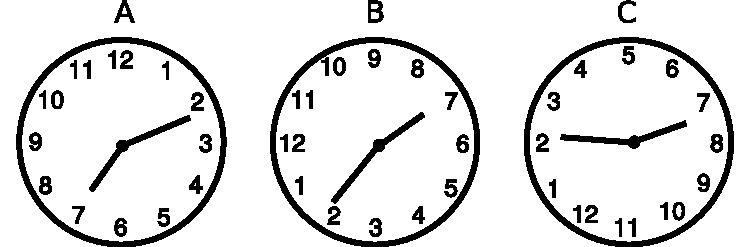
\includegraphics[width=0.7\linewidth]{figures/clock.pdf}
\end{center}
   \caption[Standards in clock design.]{Standards in clock design. The time is 07:11 (A) Modern standard, read clockwise and 12 o' clock is at North (B) Anticlockwise and 9 o' clock at North (C) Read clockwise but 5 o' clock is at North. Adapted from \cite{norman2013design}.}
   \label{fig:clock_standards}
\end{figure}
 
The \ac{BIDS} format~\citep{gorgolewski2016brain} is indeed designed with these considerations in mind. 
The standard involves a hierarchy of folders to describe the imaging technology used, the name of the subject, and the date of the experiment. 
At each level of hierarchy, files are accompanied by sidecar \code{json} files describing the metadata. 
A \code{json} file is an easy to parse text file that contains key and value pairs, so that it has the advantage of being machine and human readable at the same time. 
These files follow an \emph{inheritance principle}, that is, a field described in a \code{json} file in a higher level of the hierarchy will be automatically propagated downstream. 
The main BIDS specification is accompanied by extension specifications which describe specific aspects to describe different modalities.
At the same time, the standard does not exist in isolation.
The \ac{BIDS} consortium is also providing a growing ecosystem of tools to convert datasets into \ac{BIDS} compatible format as well as to validate data to conform to the standard. 

In the present work, we present a significant extension of \ac{BIDS} to support the specific aspects of \ac{MEG} data. \Ac{MEG}, as we know from Chapter~\ref{chapter:intro}, provides direct measurement of brain activity with millisecond temporal resolution and unique source imaging capabilities. So far, \ac{BIDS} has provided a solution to structure the organization of \ac{MRI} data, whose nature and acquisition parameters are different. Despite the lack of standard data format for \ac{MEG}, BIDS-MEG is a principled solution to store, organize and share the typically-large data volumes produced. It builds on \ac{BIDS} for \ac{MRI}, and therefore readily yields a multimodal data organization by construction. This is particularly valuable for the anatomical and functional registration of \ac{MEG} source imaging with \ac{MRI}. With BIDS-MEG and a growing range of software adopting the standard, the \ac{MEG} community has a solution to minimize curation overheads, reduce data handling errors and optimize usage of computational resources for analytics. The standard also includes well-defined metadata, to facilitate future data harmonization and sharing efforts, and extensions to other electrophysiological data modalities. 

\noindent\fcolorbox{white}{lightgray}{%
\begin{minipage}{\dimexpr\textwidth-2\fboxrule-2\fboxsep\relax}
\begin{itemize}[align=left, leftmargin=10pt, labelwidth=5pt, labelindent=10pt, itemsep=5pt, topsep=5pt]
  \item[] Section~\ref{sec:bids_intro} to Section~\ref{sec:bids_discussion} was published in:
  \item \bibentry{galan2017meg}
\end{itemize}
\end{minipage}}%

\clearpage
\section{Introduction}
\label{sec:bids_intro}
The Brain Imaging Data Structure (BIDS) is an emerging standard for the organization of neuroimaging data1. The significance of BIDS is timely: there is increasing availability of open neuroimaging data resources, and strong interest in aggregating large, heterogeneous datasets to harness machine learning techniques and address a new range of scientific questions, with greater statistical power. A single neuroimaging study by itself can represent a large and intricate volume of data, with multiple protocols and modalities, and several categories of participants possibly enrolled in repeated sessions. These aspects are challenging to data organization, harmonization and sharing. The situation is aggravated by the lack of a unique neuroscience standard for digital data across, and sometimes within, modalities such as electrophysiology. Consequently, present data management practices are often based on solutions that do not generalize between labs, or even between persons within the same group. This leads to suboptimal usage of human (time lost retrieving data), infrastructure (data storage space) and financial (limited longevity and value of disorganized data after first publication) resources. Poor or lacking data management strategies also negatively affects the reproducibility of results, even within the lab where the data were collected. 
BIDS is a standard to describe the organization of \ac{MRI} data. It is based on a simple, hierarchical folder structure, with key study parameters documented in text-based metadata files. One benefit is the handling of multiple MRI data sequences, with minimal curation overheads, which reduces the possibility of data-handling errors. An important secondary outcome is the facilitation of interoperability between tools for data analytics, provided that software and pipelines adopt BIDS for data inputs. 

We describe here a key extension of BIDS to electrophysiology data. The technical sophistication of MEG makes it the most challenging electrophysiology data type for standardization~\citep{baillet2017magnetoencephalography}. For this reason, BIDS-MEG can readily be generalized to electroencephalography, multiunit recordings, and local field potentials. Further to strengthening and rationalizing data management in MEG labs, BIDS-MEG provides a common structure to present and future large MEG open-data repositories~\citep{larson2013adding, taylor2015cambridge, niso2016omega}. The absence of unique data file format in MEG is compensated by BIDS-MEG’s standard data organization: the sharing and processing of large and complex data hierarchies is simplified, and made compatible and reproducible across tools for data analytics. 

To derive the BIDS-MEG specifications, we have combined perspectives from investigators, technical support staff and data managers. We also involved the expertise of leading academic software developers for MEG science~\citep{baillet2011academic}, including Brainstorm~\citep{tadel2011brainstorm}, FieldTrip~\citep{oostenveld2010fieldtrip}, MNE~\citep{mne}, and SPM~\citep{litvak2011eeg}. The proposed BIDS-MEG specifications are presently compatible with these software applications and toolboxes.

\section{Technical specification}
\label{sec:BIDS-MEG}

\begin{figure}[htb!]
\begin{center}
   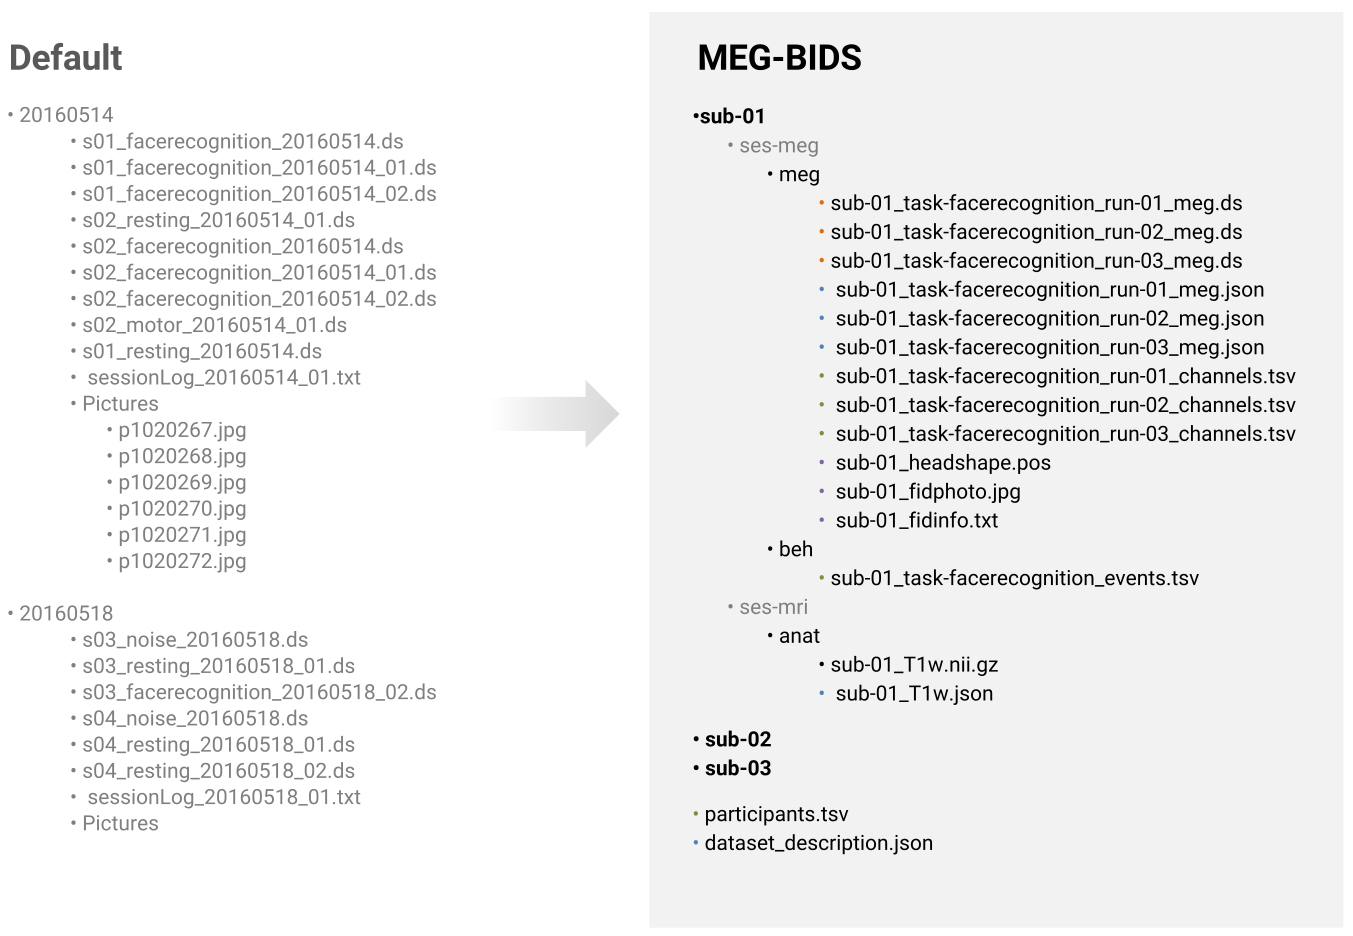
\includegraphics[width=\linewidth]{figures/bids_organization.png}
\end{center}
   \caption[BIDS-MEG data organization scheme.]{BIDS-MEG data organization scheme: Left: a typical default data organization scheme where folder are organized by date of session and contain different runs for a given participant in a study. Right: BIDS-MEG organizes data per study, then participant (subject), followed by modality, then sessions and eventually, runs. Note the sidecar files that are present at all level the data hierarchy, and document conveniently the metadata contents.}
   \label{fig:BIDS-MEG-organization}
\end{figure}


\begin{sidewaysfigure}[htb!]
\begin{center}
   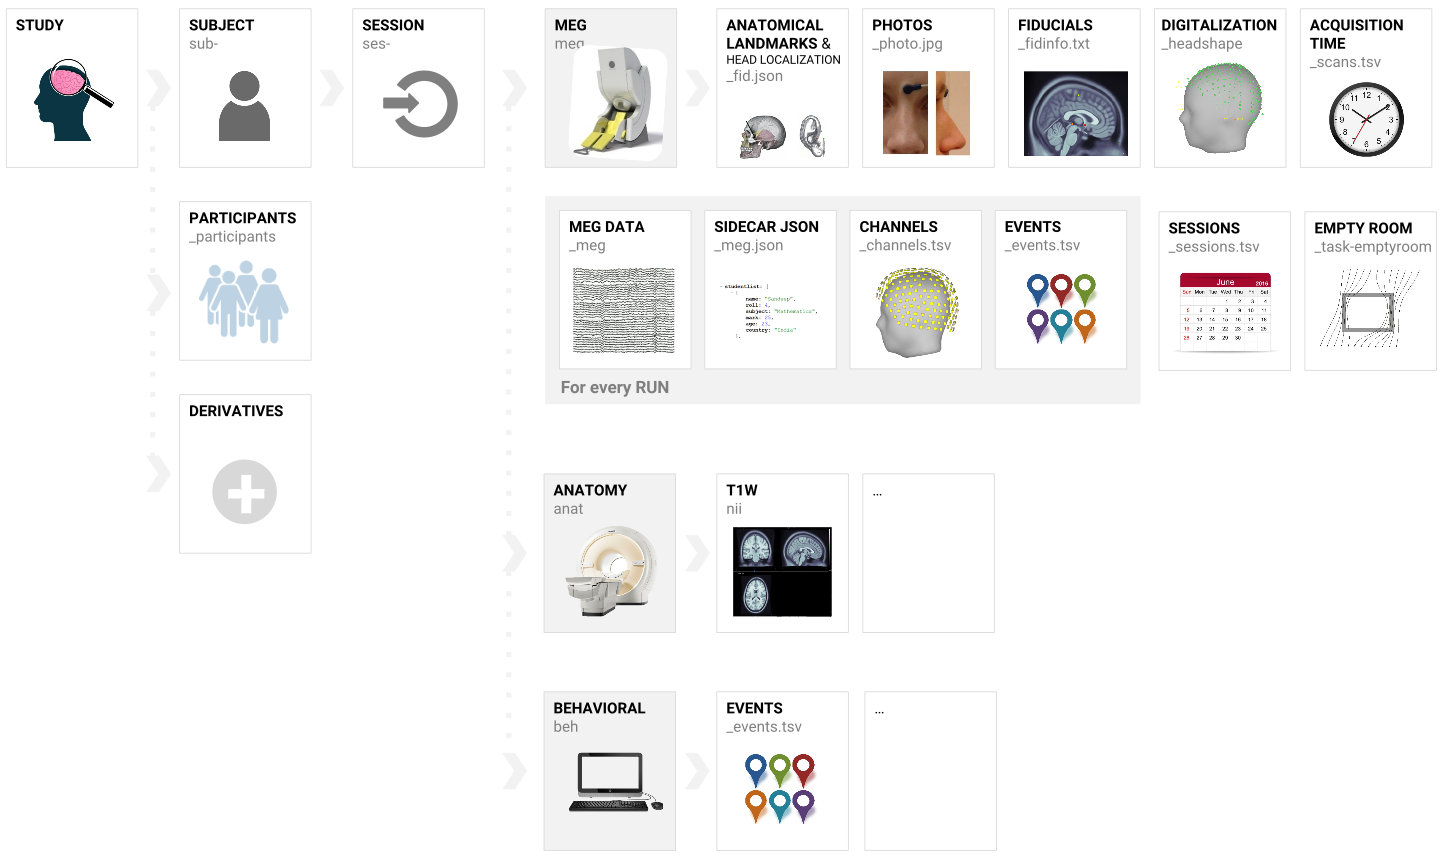
\includegraphics[width=\linewidth]{figures/bids_structure.png}
\end{center}
   \caption[BIDS-MEG general overview]{ BIDS-MEG general overview}
   \label{fig:BIDS-MEG-overview}
\end{sidewaysfigure}

\begin{sidewaysfigure}[htb!]
\begin{center}
   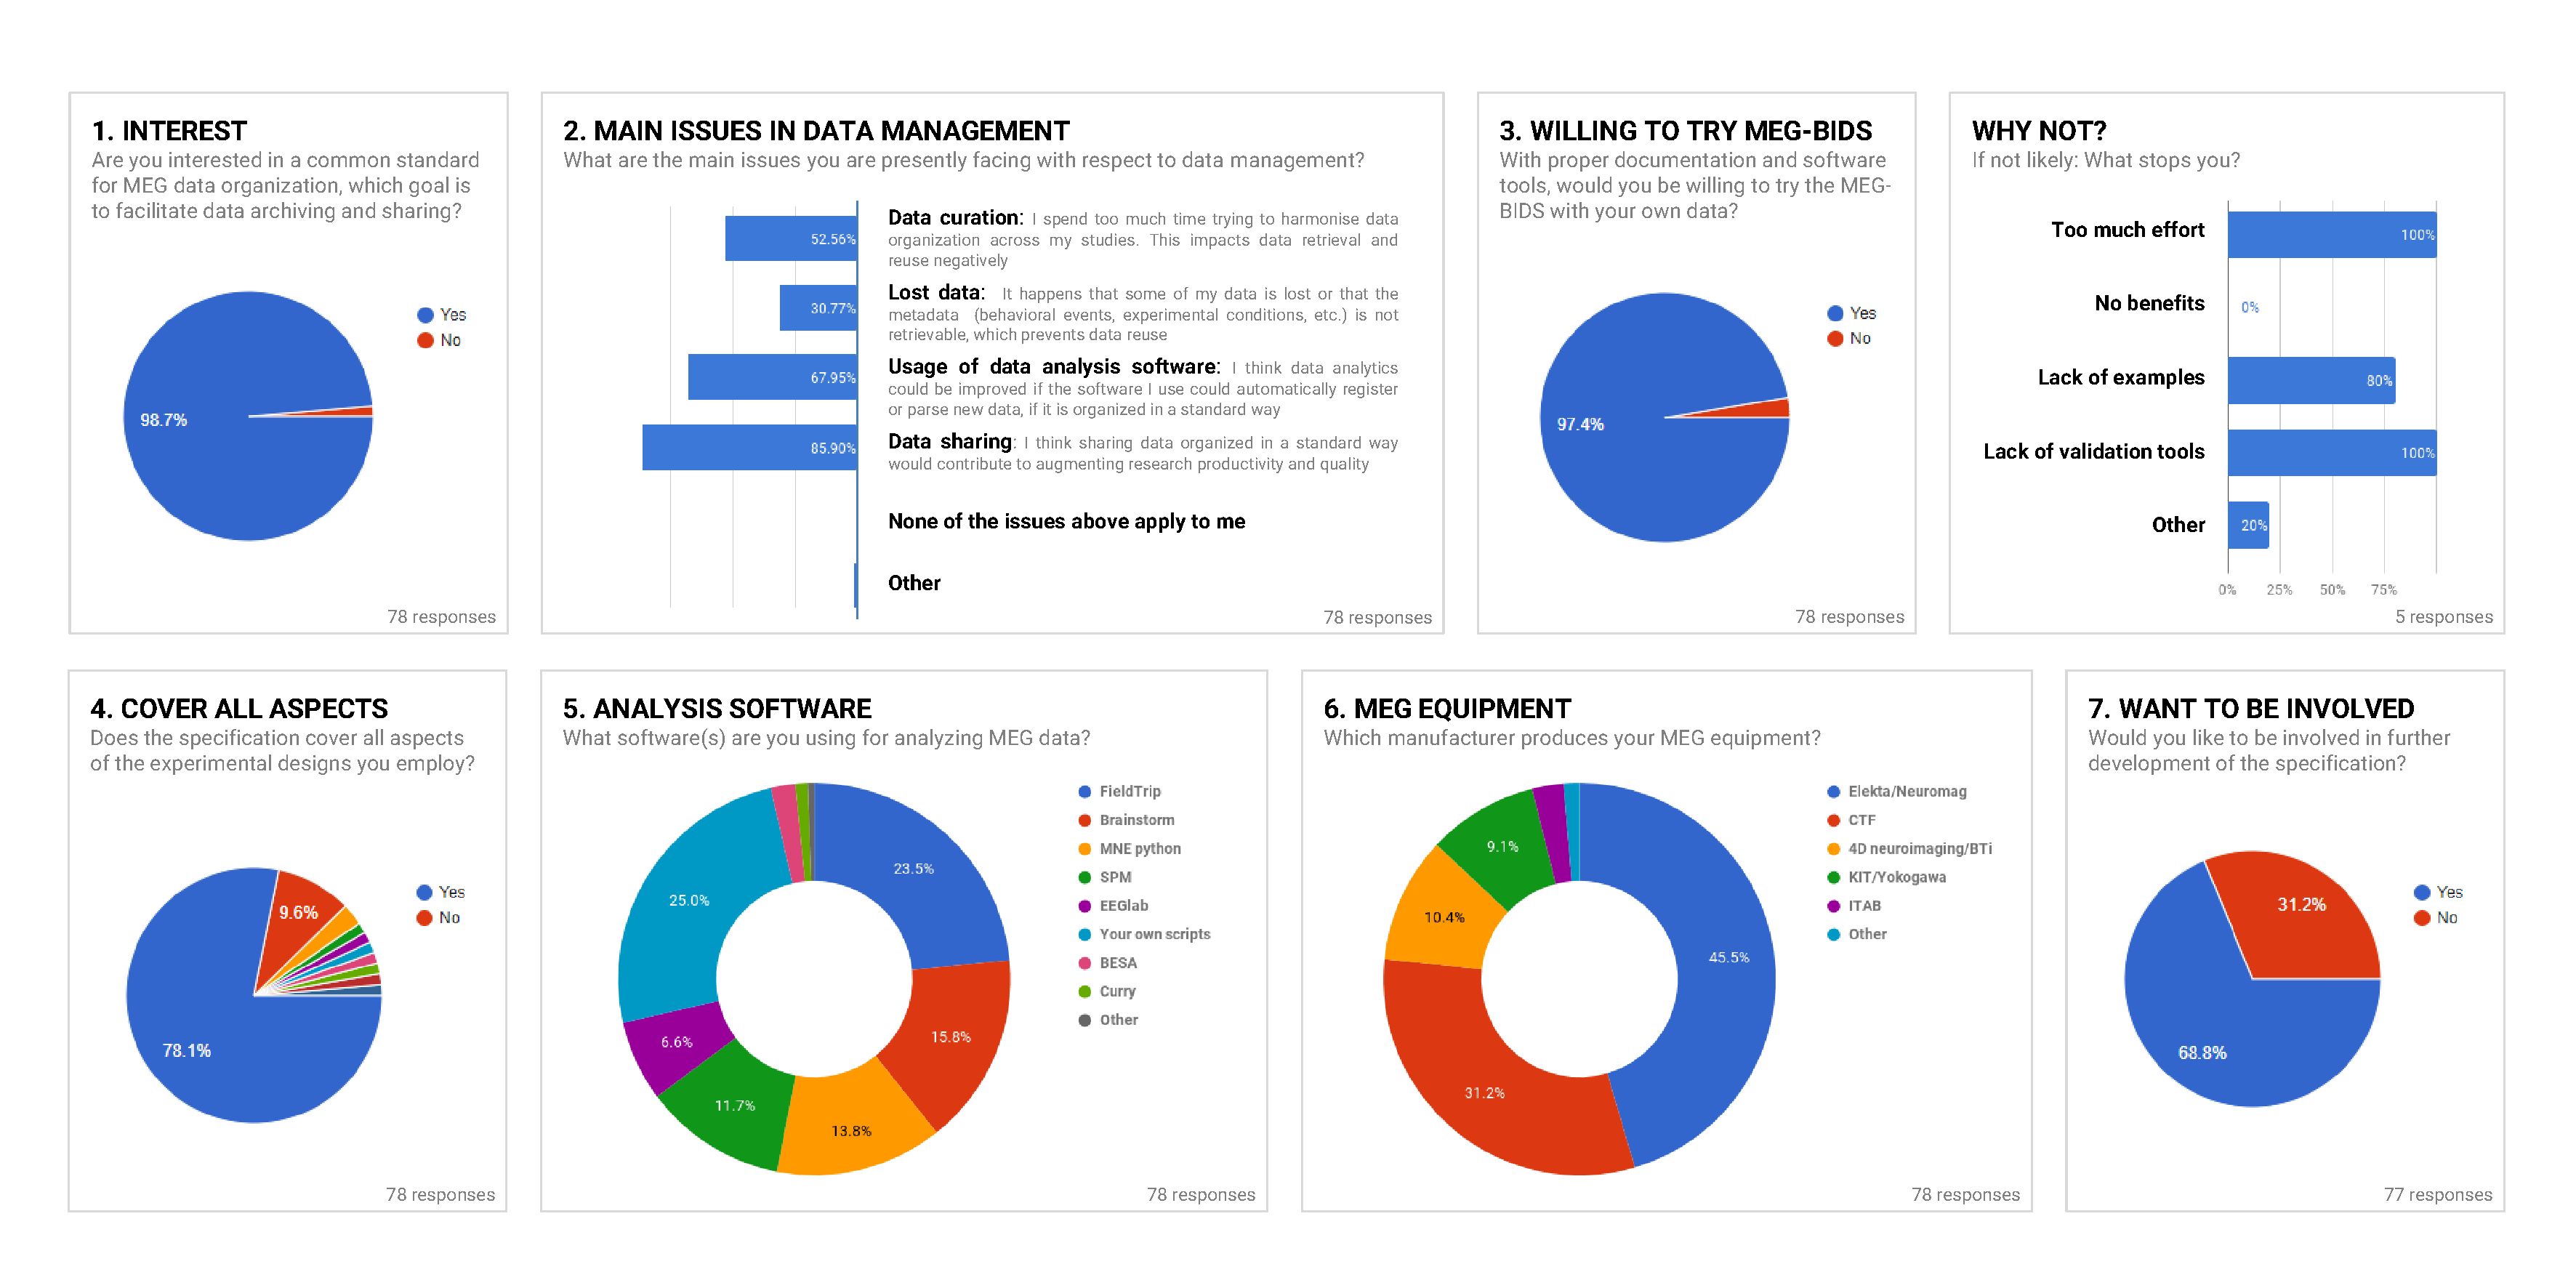
\includegraphics[width=\linewidth]{figures/MEG-BIDS_poll_results_figure.pdf}
\end{center}
   \caption[Results from the BIDS-MEG poll.]{Results from the BIDS-MEG poll}
   \label{fig:BIDS-MEG-poll}
\end{sidewaysfigure}

The BIDS-MEG fields and data organization were defined, bearing in mind best-practice guidelines for conducting MEG research~\citep{gross2013good}. The initiative fostered contributions from multiple MEG experts, with a face-to-face discussion at the 2016 International Conference on Biomagnetism, where the first incarnation of BIDS-MEG was introduced~\citep{niso2016megbids}. The first set of feedback comments and the minutes from further group discussions are publicly available
(\url{https://groups.google.com/d/msg/bids-discussion/xTHBsGhu0hk/MN25xbxRBwAJ}).

A first version of the present manuscript was shared via the preprint server bioRxiv, from where more comments stemming from the community were collected and considered for improvement of BIDS-MEG. A poll survey to probe the interest of the concerned community was also conducted (see Figure~\ref{fig:BIDS-MEG-poll}).

BIDS-MEG builds on the BIDS hierarchical data structure (see Figure~\ref{fig:BIDS-MEG-organization} and \ref{fig:BIDS-MEG-overview}). For instance data descriptors such as subject, session, technique, run are BIDS notions that were re-used in BIDS-MEG. Similarly, the simple although extensively used human and machine readable file formats (\ac{JSON}, and \ac{TSV} text files) that contributed to the versatility and practicality of documenting metadata elements in BIDS, were expanded with BIDS-MEG. BIDS-MEG employs a straightforward terminology, cautiously defined in line with the general BIDS specifications, although adapted to the unique requirements of MEG.  For further reference, the BIDS-MEG specifications are detailed in an open-access online document:
\url{https://docs.google.com/document/d/1FWex_kSPWVh_f4rKgd5rxJmxlboAPtQlmBc1gyZlRZM)}

The terms used refer to notions that were defined by reaching a consensus amongst the BIDS-MEG contributors and the MEG community. For example, ‘Subject’ refers to the scanned participant. Note that from a technical standpoint, MEG is not a scanning technique. Yet, we used this terminology for convenience, affinity with other neuroimaging modalities, and to reflect the language used in most MEG labs. A ‘Session’ defines a non-intermittent period of time during which the subject is in the scanner.  A ‘Run’ is a period of time during which empty-room (for noise characterization) or brain activity is recorded continuously, with no interruptions. It is typical with MEG that a session consists of multiple runs: task instructions can change and/or participants can take a break between runs. The notion of ‘Task’ refers to the instructions (and corresponding stimulus material) that are performed by the participant. ‘Responses’ is a feature to indicate the recorded behaviour of the subject in relation to the task.

As with the general BIDS specifications~\citep{gorgolewski2016brain}, BIDS-MEG file names are constituted by a series of key-value pairs, with multiple possible file types. Some  typological aspects are mandatory, while others remain optional, although required to abide to the BIDS guidelines. BIDS-MEG can therefore register data of any kind, including but not limited to task-based, resting-state, and empty-room MEG recordings (e.g., for noise estimation purposes). We emphasize that all of the above notions apply also to EEG, and all modalities of electrophysiology, for which BIDS-MEG serves as template for standardization.  

There is no common, open or standard file format in MEG, equivalent to DICOM or NIfTI in MRI. MEG systems manufacturers (CTF, Elekta/Neuromag, BTi/4D Neuroimaging, KIT/Yokogawa/Ricoh, Tristan Technologies, ITAB, KRISS/Compumedics Neuroscan, York Instruments) all cater a vendor-specific format. With BIDS-MEG, unprocessed (raw) data is stored in the native file format (see Discussion for further consideration of common MEG format initiatives) and users can still rely on their preferred data analysis application, possibly provided by the MEG vendor, to browse and read in the MEG file contents. Software can also extract meta information elements from the raw data files. They concern e.g., data collection parameters and other study descriptors, which are eventually transcribed into sidecar JSON files by said BIDS-MEG compatible applications. One major benefit of metadata extraction is the facilitation of subsequent data searches and indexation, without the handling and repeated parsing of large raw data files. Additional relevant files can be included alongside the MEG raw data: some propositions are detailed in the online specifications.

For a given investigator or research group, BIDS-MEG describes a hierarchical structure that descends from a ‘Study’ folder. Multiple ‘Subject’ subfolders contain the data from the participants enrolled. They are arranged by ‘Session’, each session subfolder containing ‘Run’ folders and eventually, data and metadata files. 

The ‘Run’ folder includes a variety of files: MEG recording files in native format, a sidecar JSON document (\code{*\_meg.json}), a channel description table (\code{*\_channel.tsv}), and other general BIDS files, such as task events tables (\code{*\_events.tsv}) that are likely to be specific of each run. ‘Session’ specific files include the coordinates of anatomical landmarks and head-localization coils stored in a JSON document (\code{*\_fid.json}), optional photographs of the anatomical landmarks and/or head localization coils  (\code{*\_photo.jpg}), fiducials information (\code{*\_fidinfo.txt}), 3-D scalp digitalization files (\code{*\_headshape.<manufacturer\_specific\_format>}) and acquisition times (\code{scans.tsv}). The ‘Subject’ and ‘Study’ specific files are inherited directly from the general BIDS specifications (e.g., participants.tsv). Note that in case of conflict between fields of different runs/sessions, it the inheritance principle should be applied: the description file closer to the data prevails (see Section ‘3.5 The Inheritance Principle’ of the BIDS specifications~\citep{gorgolewski2016brain}.

One issue that required special attention was the multiplicity of coordinate systems and units between MEG systems. To impose a unique coordinate system for BIDS based on the subjects’ brain anatomy (e.g., MNI coordinates or equivalent) was an appealing solution, which however would lack generalizability in the MEG practice. MEG data can be collected without anatomical information, such as empty-room noise recordings, which are important to optimal source modeling~\citep{gross-etal:13}. BIDS-MEG therefore associates all recordings with a coordinate file defined according to the MEG system used. Again, BIDS-MEG compatible software can read and interpret this information properly.

Akin to MRI, we anticipate that the systematic data organization enabled by BIDS-MEG will be supported by an increasing number of neuroimaging tools, and that more shared data repositories will be organized accordingly. The straightforward design of BIDS-MEG makes it an interoperable common exchange format for transferring data between investigators and community repositories e.g., OMEGA~\citep{niso2016omega} and OpenfMRI~\citep{poldrack2017openfmri}. It also facilitates multimodal integration (between MRI, fMRI, MEG, etc), as the data from multiple modalities follow the same organization scheme.

\section{Open BIDS-MEG datasets}
We provide four different publically-available datasets in BIDS-MEG format ($\sim$200GB). They are freely available for download from the International Neuroinformatics Coordinating Facility (INCF)’s  GitHub: \url{https://github.com/INCF/BIDS-examples/tree/bep008_meg}

The BIDS-MEG sample data release includes: 

\paragraph{OMEGA Resting-State samples:} Five minutes of eyes-open, resting-state MEG data is available for 5 subjects from The Open MEG Archive (OMEGA)~\citep{niso2016omega}. The data are available from the Brainstorm Tutorial: MEG resting state \& OMEGA database. The first release of data in BIDS-MEG format ($\sim$10.5GB) available here: 
\url{https://box.bic.mni.mcgill.ca/s/omega?path=\%2FContributions
\%20(in\%20BIDS\%20format)\%2Fsample_BIDS_omega} (access to these datasets require registration to OMEGA, \url{https://www.mcgill.ca/bic/omega-registration}).

\paragraph{Brainstorm Auditory Example dataset:} Brainstorm Auditory tutorial dataset8 ($\sim$2.3GB):
\url{https://box.bic.mni.mcgill.ca/s/omega?
path=\%2FContributions\%20(in\%20BIDS\%20format)
\%2Fsample_BIDS_auditory} (released in Public Domain; includes defaced anatomical T1 of participant, access to these datasets require registration to Brainstorm, \url{http://neuroimage.usc.edu/bst/register.php}). 

\paragraph{MNE Sample data:} Sample data with visual and auditory stimuli described in11:
\url{https://drive.google.com/drive/folders/0B_sb8NJ9KsLUQ3BMS0dxZW5nSHM?usp=sharing} (released in Public Domain; includes anatomical T1 of participant as well as flash MRI sequences). 

\paragraph{OpenfMRI study ds000117:} A multi-subject, multi-modal human neuroimaging dataset of 19 subjects participating in a visual task16 ($\sim$178GB): \url{https://openfmri.org/dataset/ds000117/}. This dataset is used in one of the SPM tutorials, for training purposes:
\url{http://www.fil.ion.ucl.ac.uk/spm/doc/manual.pdf#Chap:data:multimodal}

\section{Software}
Widely used MEG software packages have already added functionality to support BIDS-MEG:

\paragraph{Brainstorm}\citep{tadel2011brainstorm}: Brainstorm is an application with rich graphical-user interactions and analytic pipeline designs for MEG, EEG, NIRS, and electrophysiology recordings. BIDS-formatted MEG/EEG datasets can be imported automatically into the Brainstorm database, as described in the OMEGA tutorial: \url{http://neuroimage.usc.edu/brainstorm/Tutorials/RestingOmega}

\paragraph{FieldTrip}\citep{oostenveld2010fieldtrip}: FieldTrip is an open-source MATLAB toolbox for the analysis of MEG, EEG, and other electrophysiological data. Like most other tools listed herewith, FieldTrip can  implement full analysis pipelines, starting from coregistration, preprocessing, time- and spectral analysis, source reconstruction, connectivity and statistics. Among others, FieldTrip has been used for the MEG part of the Human Connectome Project. Since a FieldTrip analysis pipeline is represented as a MATLAB script, its application on BIDS structured data implies that the BIDS details are represented in the analysis scripts that users write. 

\paragraph{MNE}\citep{gramfort2013meg, mne}: MNE (\url{http://martinos.org/mne}), whose name stems from its capability to compute cortically-constrained minimum-norm current estimates from M/EEG data. It is a software package that provides comprehensive analysis tools and workflows including preprocessing (Maxwell filtering, ICA, signal space projectors), source estimation (eg. using MNE, beamformers or mixed-norm sparse solvers), time-frequency analysis, statistical analysis including multivariate decoding, and several methods to estimate functional connectivity between distributed brain regions. The core of MNE is written in Python and is distributed under the permissive BSD Licence. MNE will use the BIDS data structure to distribute all its tutorial datasets and the documented analysis scripts. MNE provides Python code to read and write files in BIDS compatible format, as well as summary reports automatically generated via the MNE report command. A preliminary version is available at \url{https://github.com/mne-tools/mne-bids}. 

\paragraph{SPM}\citep{litvak2011eeg}: SPM (\url{http://www.fil.ion.ucl.ac.uk/spm}) is a free and open source software written in MATLAB where many widely used methods for the analysis of PET, fMRI and for computational neuroanatomy have been originally developed and implemented. More recently SPM has been extended to perform M/EEG analyses, including topological inference for neurophysiological data, empirical Bayesian framework for source reconstruction and Dynamic Causal Modeling (DCM), an approach combining neural modeling with data analysis. SPM~\citep{litvak2011eeg} includes a library, spm\_BIDS.m, to parse and query BIDS-formatted datasets, as well as low-level functions to read/write JSON and TSV metadata files. A complete pipeline for the analysis of a group MEG dataset in BIDS format is presented in preparation.

\paragraph{Other BIDS-MEG tools:}

Another set of tools have been developed to generate sidecar BIDS-MEG JSON files, and assist researchers in their evaluation  and adoption of the standard. These Python scripts are publicly available:  \url{https://github.com/INCF/pybids}.

For a more detailed description of the BIDS-MEG specification, example datasets, resources and feedback, please visit \url{http://bids.neuroimaging.io}.

\section{Discussion}
\label{sec:bids_discussion}
Although BIDS-MEG is a proposal to establish a standard framework for the organization of electrophysiology data, it does not impose the standardization of the data file format per se. Some initiatives are aiming towards the definition of a new common binary file format for electrophysiology (MNE python group). Akin to DICOM in MRI, one single file format would beneficial, when considering the diversity of native raw file formats in electrophysiology. Yet, MEG data volumes are typically very large (several GBs), hence their duplication into a standard format may be unimpractical. Our position is rather to promote BIDS-MEG and ascertain that tools for data analytics continue to be equipped with the necessary readers for all existing vendor formats. We believe the capacity of BIDS-MEG to organise data without requiring a common data format is actually a strength: the standard is flexible in the sense that any data parameters can be extracted and stored as metadata in sidecar json files at the time of creating a new data entry, regardless of the file format for the raw data. Therefore, any new data format for electrophysiology, including emerging standards, is by construction compatible with BIDS-MEG.

Along the same lines, special attention was given to the handling of the various  coordinate systems used by the different MEG vendors and toolboxes. BIDS-MEG is also flexible in that respect, as long as the conventions used are characterized and documented in the \code{*\_fid.json} file. The coordinate systems presently handled by BIDS-MEG are detailed in the Specification document. The coordinate systems used for MEG and EEG sensors, MRI volumes, locations of fiducials, anatomical landmarks and digitized head points, need to be described following this principle, as some are likely to be different.

We aim at extending BIDS-MEG further towards the handling of processed data, which for now and akin to MRI-BIDS, are simply stored in a data Derivatives folder.

BIDS-MEG represents a significant effort towards a common standard for MEG. We anticipate that the BIDS-MEG software ecosystem and the variety of publicly available BIDS-MEG datasets will grow and incentivize the research community towards adoption. 


\acresetall % reset acronyms for chapter
\chapter{A reproducible M/EEG group study}
\label{chapter:group_study}
%\epigraph{\small\itshape ``The first principle is that you must not fool yourself – and you are the easiest person to fool.''}{\small\textit{---Richard Feynman}}

\vspace{20pt}
\epigraph{\small\itshape ``Extraordinary claims require extraordinary evidence.''}
{\small\textit{---Carl Sagan}}

\begin{figure}[ht!]
\centering
\begingroup
\etocstandardlines
%\renewcommand{\etocbkgcolorcmd}{\color{lightgray}}
\renewcommand{\etocbelowtocskip}{0pt\relax}
\fboxsep1ex
\etocframedstyle [1]{\fbox{\makebox[.4\linewidth]{\etocfontminusone
Contents}}}
\localtableofcontents
\endgroup
\end{figure}

% General structure of each section (ideally)
% - Here is what we did
% - Why it makes sense? (figure)
% - This is how we checked that what we did makes sense
In the previous chapter, we discussed how data sharing can be facilitated using the \ac{BIDS} for \ac{MEG}. This is taking us one step closer to the goal of reproducible. However, reproducibility is not achieved by merely sharing more data with the hope that this will solve all problems. As noted in \citet{baker20161}, one of the best solutions to foster reproducible science is not a technical one, but an educational one. This is true for statistics, which is not always well-understood but also for academic software.

In recent years, free academic toolboxes have gained increasing prominence in \ac{MEG} analysis as a means to disseminate cutting edge methods, share best practices between different research groups and pool resources for developing essential tools for the \ac{MEG} community. Teaching events are regularly held around the world where the basics of each toolbox are explained by its respective developers and experienced power users. There are however, knowledge gaps that need to be addressed. First, most teaching examples only show analysis of a single ‘typical best’ subject whereas most real MEG studies involve analysis of group data. It is then left to the researchers in the field to figure out for themselves how to make the transition and obtain significant group results. Secondly, we are not familiar with any examples of fully analyzing the same group dataset with different academic toolboxes to assess the degree of agreement in scientific conclusions and compare strengths and weaknesses of various analysis methods and their independent implementations.

To address this very issue, a workshop was organised by the lead developers of six most popular free academic MEG toolboxes at Biomag 2017. This work is a follow up to the workshop, which presents the MNE contribution, and will be published in \emph{Frontiers in Neuroscience, section Brain Imaging Methods}. This study presents the results obtained by the reanalysis of an open dataset from \citet{wakeman2015multi} using the MNE software package. The analysis covers preprocessing steps, quality assurance steps, sensor space analysis of evoked responses, source localization, and statistics in both sensor and source space. Results with possible alternative strategies are presented and discussed at different stages such as the use of high-pass filtering versus baseline correction, tSSS versus \ac{SSS}, the use of a minimum norm inverse versus \ac{LCMV} beamformer, and the use of univariate or multivariate statistics. This aims to provide a comparative study of different stages of \ac{MEG}/\ac{EEG} analysis pipeline on the same dataset, with open access to all of the scripts necessary to reproduce this analysis.

\noindent\fcolorbox{white}{lightgray}{%
\begin{minipage}{\dimexpr\textwidth-2\fboxrule-2\fboxsep\relax}
\begin{itemize}[align=left, leftmargin=10pt, labelwidth=5pt, labelindent=10pt, itemsep=5pt, topsep=5pt]
  \item[] Section~\ref{sec:group_study_intro} to Section~\ref{sec:group_study_discussion} was published in:
  \item \bibentry{jas2017mne}
\end{itemize}
\end{minipage}}%

\clearpage
\section{Introduction}
\label{sec:group_study_intro}

\Ac{MEG} and \ac{EEG} are neuroimaging technologies with a high temporal resolution, which provide non-invasive access to population-level neuronal dynamics on virtually any temporal scale currently considered relevant to cognition. % DE that is actually an important point to make. It's a distinct feature of the technology.
While MEG can recover spatial patterns at a higher \ac{SNR} and enjoys a more selective cortical resolution than \ac{EEG}~\citep{baillet17}, EEG is more portable and less expensive, and thus supports the study of cognition in a wider range of situations. Processing M/EEG recordings, however, is inherently challenging due to the multi-dimensional nature of the data, the low \ac{SNR} of brain-related M/EEG signals, and the differences in sensitivity of these measurement techniques. This can give rise to complex sequences of data processing steps which demand a high degree of organization from the investigator.

In an effort to address reproducibility issues recently shown to affect neuroimaging studies~\citep{ioannidis2005most, button2013power,Carp2012,Carp2012289}, a number of community-led efforts have begun developing data sharing~\citep{poldrack2017openfmri} and data organization~\citep{gorgolewski2016brain, galan2017meg} projects. These efforts are necessary first steps, but are not sufficient to solve the problem---they must be complemented by educational tools and guidelines that establish good practices for M/EEG analysis~\citep{gross-etal:13}. However, putting guidelines into practice is not always straightforward, as researchers in the M/EEG community rely on several software packages~\citep{tadel2011brainstorm,delorme2004eeglab,eeglab2,
oostenveld2010fieldtrip,nutmeg,litvak2011eeg}, each of which is different. Even though these packages provide tutorials for single subject data analysis, it is typically left up to the investigator to coordinate and implement multi-subject analyses. Here, we try to address this gap by demonstrating a principled approach to the assembly of group analysis pipelines with publicly available code\footnote{\url{https://github.com/mne-tools/mne-biomag-group-demo}} and extensive documentation. 

As members and maintainers within the MNE community, we will present analyses that make use of the MNE software suite~\citep{mne}. Historically, MNE was designed to calculate minimum-norm estimates from M/EEG data, and consisted in a collection of C-routines interfaced through bash shell scripts. Today, the MNE software has been reimplemented in~\citep{gramfort2013meg} and transformed into a general purpose toolbox for processing electrophysiology data. Built on top of a rich scientific ecosystem that is open source and free, MNE now offers state-of-the-art inverse solvers and tools for preprocessing, time-frequency analysis, machine learning (decoding and encoding), connectivity analysis, statistics, and advanced data visualization. MNE, moreover, has become a hub for researchers who use it as a platform to collaboratively develop novel methods or implement and disseminate the latest algorithms from the M/EEG community~\citep{engemann2015automated, smith2015regression1, smith2015regression2, haufe2014interpretation, king2014characterizing, gramfort-etal:2013, schurger2013reducing, khan2013note, larson_cortical_2012, hauk2011comparison, gramfort2010graph, rivet2009xdawn, kriegeskorte2008representational, maris_nonparametric_2007}. With this work, we not only  share best practices to facilitate reproducibility, but also present these latest advances in the MNE community which enable automation and quality assessment.

Here, we demonstrate how to use MNE to reanalyze the OpenfMRI dataset ds000117 by~\cite{wakeman2015multi}. This requires setting the objectives for the data analysis, breaking them down into separate steps and taking a series of decisions on how to handle the data at each of those steps. While there may be several interesting scientific questions that have not yet been addressed on this dataset, here we confine ourselves to the analysis of well-studied time-locked event-related M/EEG components, i.e, \acp{ERF} and \acp{ERP}. This is motivated by educational purposes to help facilitate comparisons between software packages and address reproducibility concerns. To this end, we will lay out all essential steps from single subject raw M/EEG recordings to group level statistics. Importantly, we will highlight the essential options, motivate our choices and point out important quality control objectives to evaluate the success of the analysis at every step.

We will first analyze the data in sensor space. We will discuss the best practices for selecting filter parameters, marking bad data segments, suppressing artifacts, epoching data into time windows of interest, averaging, and doing baseline correction. Next, we turn our attention to source localization: the various steps involved in the process starting from defining a head conductivity model, source space, coregistration of coordinate frames, data whitening, lead field computation, inverse solvers, and transformation of source-space data to a common space. Along the way, we will present various diagnostic visualization techniques that assist quality control at each processing step, such as channel-wise \ac{PSD}, butterfly plots with spatial colors to facilitate readability, topographic maps, and whitening plots. Finally, we will attempt to distill from our analysis, guiding principles that should facilitate successfully designing \textit{other} reproducible analyses rather than blindly copying the recipes presented here. 

\section{Preliminaries}

In this work, we describe a full pipeline using MNE to analyze the OpenfMRI dataset ds000117 by~\cite{wakeman2015multi}. The data consist of simultaneous M/EEG recordings from 19 healthy participants performing a visual recognition task. Subjects were presented images of famous, unfamiliar and scrambled faces. The dataset provides a rich context to study different neuroscientific and cognitive questions, such as: Which brain dynamics are characteristic of recognizing familiar as compared to unfamiliar faces? How do commonly studied face-responsive brain regions such as the \ac{STS}, the \ac{FFA} and the \ac{OFA} interact when processing the familiarity of the face? At the same time, it presents a well-studied paradigm which can be particularly beneficial for the development of methods related to connectivity and source localization.

\subsection{Data description}

The subjects participated in 6 runs, each 7.5 minutes in duration. In the original study, three subjects were discarded due to excessive artifacts in the data. To produce comparable results, the same subjects are also discarded from the group results in this study. The data were acquired with an Elekta Neuromag Vectorview 306 system consisting of 102 magnetometers and 204 planar gradiometers. In addition, a 70 channel Easycap EEG system was used for recording EEG data simultaneously.

\subsection{Reading data}
MNE supports multiple file formats written by M/EEG hardware vendors.
Apart from Neuromag \textit{FIF} files, which are the default storage format, MNE can natively read multiple other formats ranging for MEG data including 4D Neuroimaging BTI, KIT, and CTF, and for EEG data B/EDF, EGI, and EEGLAB \textit{set}\footnote{\url{http://martinos.org/mne/stable/manual/io.html}}. Despite this heterogeneity of systems, MNE offers a coherent interface to the metadata of the recordings using the so-called \emph{measurement info}\footnote{\url{http://martinos.org/mne/stable/auto_tutorials/plot_info.html}}.
Regardless of the input format, all processed files can be saved as \textit{FIF} files or in the HDF5 format\footnote{\url{https://support.hdfgroup.org/HDF5/}}.

MNE can handle multimodal data containing different channel types, the most common being magnetometer, gradiometer, \ac{EEG}, \ac{EOG}, \ac{ECG}, and stimulus trigger channels that encode the stimulation paradigm. MNE also supports \ac{EMG}, stereotactic EEG (sEEG) and electrocorticography (ECoG), \ac{fNIRS} or miscellaneous (misc) channel types. Declaring and renaming channel types is a common step in the preparation of M/EEG datasets before analysis. In our case, once the files were read in, some of the channels needed to be renamed and their channel types corrected in the measurement info (see~\citep{wakeman2015multi}): the EEG061 and EEG062 electrodes were set as EOG, EEG063 was set as \ac{ECG}, and EEG064 was set as a miscellaneous channel type as it was a free-floating electrode. If this step is omitted, some preprocessing functions may fall back to potentially less optimal defaults, for example, using the average of the magnetometers instead of the \ac{ECG} channel when searching for cardiac events.

\section{MEG and EEG data preprocessing}

\subsection{Maxwell filtering (SSS)}
\label{sec:maxfilter}

\begin{figure}[htb]
        \centering
        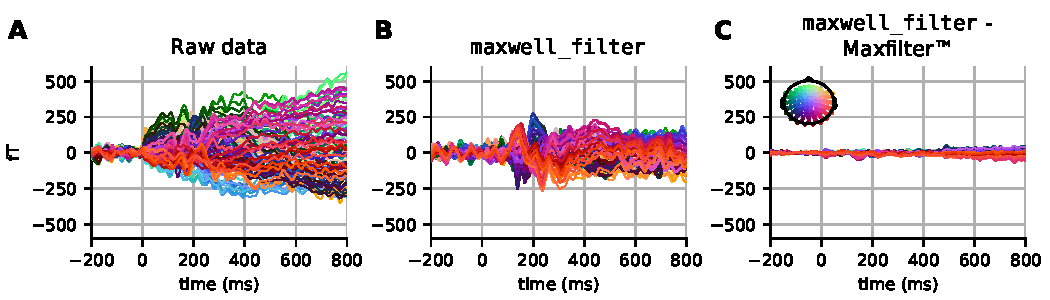
\includegraphics[width=\linewidth]{figures/Maxfilter.pdf}
        \caption[Comparison of Elekta MaxFilter (TM) and MNE implementation]{Evoked responses (filtered between 1 and 40 Hz) in the magnetometer channels from (A) unprocessed data, (B) data processed with \code{maxwell\_filter} in MNE, and (C) the difference between data processed using \code{maxwell\_filter} and Elekta MaxFilter (TM). The colors show the sensor position, with $(x, y, z)$ sensor coordinates converted to $(R, G, B)$ values, respectively.}
        \label{fig:fig_maxwell}
\end{figure}

% mj: you can also have artifacts inside the room
% In the absence of an excellent magnetically shielded room or a very quiet electromagnetic environment
Neuromag MEG recordings are often preprocessed first using the \ac{SSS} method~\citep{taulu2006spatiotemporal}, otherwise known as Maxwell filtering. \ac{SSS} decomposes the data using multipole moments based on spherical harmonics and removes the component of magnetic field originating from outside the MEG helmet. \ac{SSS} is therefore useful for removing environmental artifacts, and can also be used to compensate for head movements during the recording. In this study, movement compensation is not strictly necessary as the participants managed to stay predominantly still.

The data provided by OpenfMRI~\citep{poldrack2017openfmri} already contain files processed using the proprietary Elekta software MaxFilter, which is what we use in our analysis for the sake of reproducibility. However, MNE offers an open source reimplementation and extension of \ac{SSS} as well. Before running SSS, it is crucial that bad channels are marked, as otherwise \ac{SSS} may spread the artifacts from the bad channels to all other MEG channels in the data. This step is preferably done manually with visual inspection. When using the MNE implementation of Maxwell filtering, we reused the list of bad channels available from the Elekta MaxFilter logs in the dataset.

Results comparing raw data, data processed by Elekta MaxFilter, and data processed by the MNE \code{maxwell\_filter} function are provided in Figure~\ref{fig:fig_maxwell}. While the unprocessed data do not show a clear evoked response, the Maxwell filtered data do exhibit clear event-related fields with a clear peak around 100\,ms post-stimulus. Note that the results obtained with Elekta implementation and the MNE implementation have minimal differences due to slight differences in computation of component regularization parameters.

\emph{Alternatives} In principle, SSS can be applied to data acquired with any MEG system providing it has comprehensive sampling (more than  about 150 channels). However, so far it has not been tested extensively with other than the 306-channel Neuromag systems. SSS requires relatively high calibration accuracy, and the Neuromag systems are thus carefully calibrated for this purpose. If SSS is not an option, for example due to the lack of fine-calibration information, reasonable noise reduction can be readily obtained from \acp{SSP}~\citep{uusitalo1997signal}. This intuitively amounts to projecting out spatial patterns of the empty room data covariance matrix using \ac{PCA}. In practice, depending on the shielding of the room, up to a dozen \ac{SSP} vectors can be discarded to obtain satisfactory denoising.

\emph{Caveats}. It is important to highlight that after \ac{SSS}, the magnetometer and gradiometer data are projected from a common lower dimensional \ac{SSS} coordinate system that typically spans between 64 and 80 dimensions. As a result, both sensor types contain highly similar information, which also modifies the inter-channel correlation structure. This is the reason why MNE will treat them as a single sensor type in many of the analyses that follow.

\subsection{Power spectral density (PSD)}

\begin{figure}[htb]
        \centering
        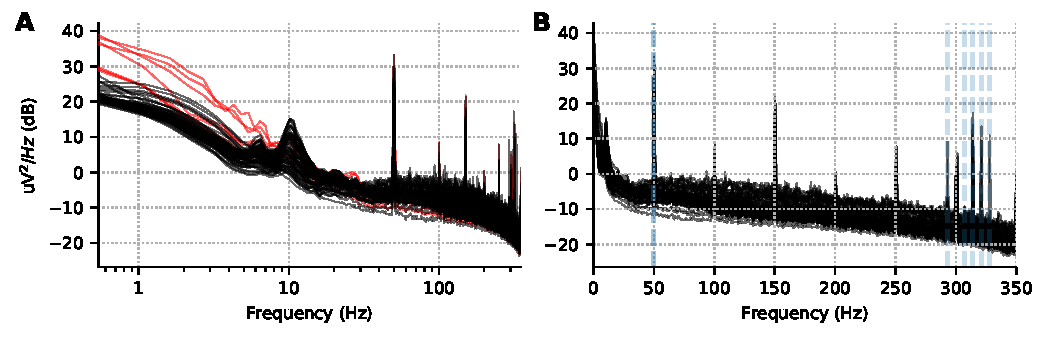
\includegraphics[width=\linewidth]{figures/psd.pdf}
        \caption[Power spectral density to mark bad channels and check filtering]{Power spectral density per channel for subject 10, run 02. (A) Log scale for the x axis accentuates low frequency drifts in the data. The red lines show the PSD for the bad channels marked manually and provided to us by~\citet{wakeman2015multi}. (B) The same data with a linear x-axis scale. Five peaks corresponding to HPI coils around 300 Hz are visible and marked in gray dotted lines alongside the power line frequency (50 Hz).}
        \label{fig:fig1_plot_psd}
\end{figure}

The \ac{PSD} estimates for all available data channels provide a convenient way to check for spectral artifacts and, in some cases, bad channels. MNE computes the PSD of raw data using the standard Welch's method~\citep{Welch67,percival1993spectral}, whereby the signal for each channel is analyzed over consecutive time segments, with eventually some overlap. Each segment is windowed and then the power of the discrete Fourier transform (DFT) coefficients is computed and averaged over all segments. By making the assumption that  each of these segments provides a realization of a stationary process, the averaging procedure produces an unbiased estimate of the PSD with reduced noise.

Starting from MNE version 0.14, we show channel-wise PSD plots rather than an average across channels, as this facilitates spotting outlier channels. In Figure~\ref{fig:fig1_plot_psd}, we show the PSD for the EEG channels in one run for one subject. We use windows of length 8192 samples (about 7.4\,s given the 1.1\,kHz sampling rate) with no overlap. Using a power of 2 for the length and no overlap accelerates computations. Using a logarithmic frequency-axis scaling for the PSD enables quality control by facilitating screening for bad channels. In fact, we found that some potentially bad channels (e.g., EEG024 in subject 14 for run 01) were omitted by the authors of \citep{wakeman2015multi}, although they are clearly visible in such plots. Concretely we see a few channels with strongly increased low-frequency power below 1 Hz. On the other hand, using a linear frequency-axis scaling, we can convince ourselves easily that the data is unfiltered, as it contains clear peaks from power line at harmonics of 50 Hz, as well as the five Head Position Indicator (HPI) coils used to monitor the head position of the subject, at frequencies of 293, 307, 314, 321, and 328\,Hz.

\emph{Alternatives} The same could have been achieved with the multitaper method~\citep{percival1993spectral, slepian1978prolate}, where the data is multiplied element-wise by orthogonal data tapers. However, this method can be an order of magnitude slower than the Welch method for long continuous recordings. The multitaper method is indeed recommended for short data segments. Here we are interested in the PSD for diagnostic purposes on the raw continuous data, and we therefore use the Welch method, a.k.a. averaged periodogram method.

\subsection{Temporal filtering}
\label{sec:group_study_temporal_filtering}

In this study, we focused on event-related brain signals below 40\,Hz. We low-pass filtered our data at a 40\,Hz cutoff frequency with 10 Hz transition band. Such a filter does not affect \ac{ERP} signals of interest, attenuates the line frequency of 50\,Hz and all HPI coil frequencies. It also limits the effects of temporal ringing thanks to a wide transition band. Because the low-pass was sufficiently low, we did not employ a notch filter separately. Note that such a choice of filters is not necessarily a good default for all studies of event-related brain responses, as ERFs or ERPs can contain rather high frequencies (see for example \citep{gotz-etal:15}).

When filtering, it is important to take into account the frequency response and impulse response of the filter. In MNE 0.16, the default filter will adapt the filter length and transition band size based on the cutoff frequencies, as done in the EEGLAB software~\citep{widmann2015digital,parks1987digital,ifeachor2002digital}\footnote{\url{https://martinos.org/mne/stable/auto_tutorials/plot_artifacts_correction_filtering.html}}. Although no default parameters will fit all analysis requirements, MNE chooses parameters that aim to achieve reasonable stop-band attenuation without excessive filter ringing. To illustrate this point, we compare filters across MNE versions using frequency response and impulse response plots in Figure~\ref{fig:fig2_filter}. The stop-band attenuation and transition bandwidth in Figure~\ref{fig:fig2_filter}A and Figure~\ref{fig:fig2_filter}B are less restricted in the newer versions, which results in less steep attenuation but also less temporal ringing in the impulse response (see Figures~\ref{fig:fig2_filter}C and D). It can be seen that the previous default parameters gave rise to stronger filtering artifacts as indicated by higher impulse response amplitudes across the time window.

\begin{figure}[htb]
    \centering
    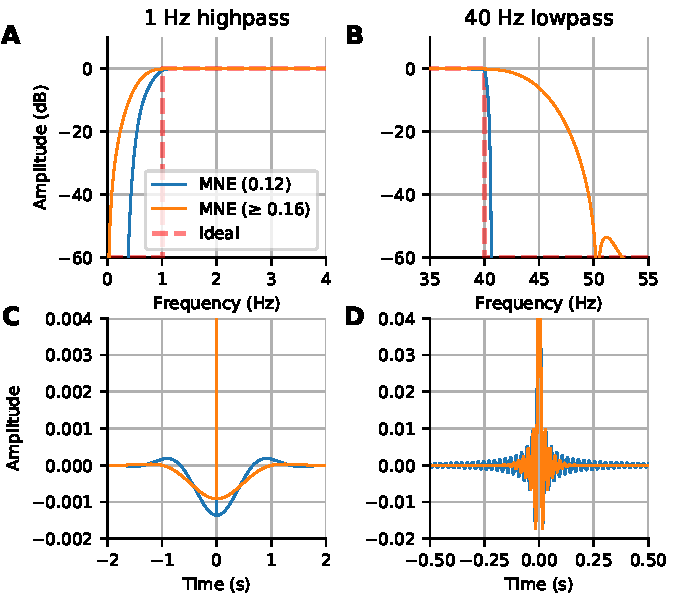
\includegraphics[width=0.8\linewidth]{figures/filters.pdf}
    \caption[Comparison of filters between new (0.16) and old (0.12) MNE versions.]{Comparison of filters between new (0.16) and old (0.12) MNE versions: (A) The frequency response of the highpass filter; (B) The frequency response of the lowpass filter; (C) The impulse response of the highpass filter; (D) The impulse response of the lowpass filter. The filters in MNE are now adaptive with trade-offs between frequency attenuation and time domain artifacts that by default adapt based on the chosen low-pass and high-pass frequencies.}
    \label{fig:fig2_filter}
\end{figure}

\emph{Alternatives and Caveats:} If the signal quality is satisfactory, filtering may not be necessary. In the context of this study, we decided to baseline correct our signals rather than high-pass filter them, keeping in mind the ongoing discussion in the community on this topic~\citep{tanner2015inappropriate,rousselet2012does,widmann2012filter,acunzo2012systematic,maess2016high}. Our choice will be motivated in Section~\ref{sec:baseline} on baseline correction.

\subsection{Marking bad segments and channels}

The next step in the pipeline is to remove bad data segments and bad channels. As data have been processed with Maxwell filter, there are no more bad \ac{MEG} channel at this stage. For the bad EEG channels, we use the ones provided by the original authors.

To remove bad data segments and bad epochs due to transient artifacts, it is possible in MNE to use the epochs plotter interactively, or to do it via scripting. Either way, the indices of all epochs that are removed from further analysis are logged in the \textit{drop log} attribute of the epochs objects (see online documentation of the Epochs class\footnote{\url{http://martinos.org/mne/stable/auto_tutorials/plot_epoching_and_averaging.html}}).

As we are building a reproducible pipeline, here we prefer the scripting route. In MNE, this can be achieved by removing trials whose peak-to-peak amplitude exceeds a certain rejection threshold. Even though this works reasonably well for single subject analysis, it would likely need to be tuned for individual subjects in group studies. Therefore, instead of specifying the thresholds manually, we learn it from the data using the \emph{autoreject} (global)~\citep{jas2017autoreject} algorithm. \emph{Autoreject} is an unsupervised algorithm which minimizes the cross-validation error, measured by the Frobenius norm between the average signal of the training set and the median signal of the validation set. \emph{Autoreject} not only removes trials containing transient jumps in isolated \ac{MEG} or \ac{EEG} channels, but also eyeblink artifacts affecting groups of channels in the frontal area. Since we are dealing with visual stimuli, it is preferable to remove the eyeblink trials altogether using the \ac{EOG} rejection threshold over the stimulus presentation interval rather than suppressing the artifact using a spatial filter such as \ac{ICA} or \ac{SSP}. Given the large number of trials at our disposal, we can afford to remove some without affecting the results very much.

For the purpose of group averaging, the bad \ac{EEG} channels were repaired by spherical spline interpolation~\citep{perrin1989spherical} so as to have the same set of channels for each subject.

\subsection{Independent Component Analysis (ICA)}
 
Bad channel or segment removal can correct for spatially and temporally isolated artifacts. However, it does not work well for systematic physiological artifacts that affect multiple sensors. For this purpose, \ac{ICA} is commonly used~\citep{jung1998extended}. \ac{ICA} is a blind source separation technique that maximizes the statistical independence between the components. While \ac{PCA} only requires orthogonal components, \ac{ICA} looks for independence for example by looking at higher statistical moments beyond (co)variance. In the context of MEG and EEG analysis, common physiological artifacts have skewed and peaky distributions, hence are easily captured by \ac{ICA} methods that look for non-Gaussian sources. \ac{ICA} is therefore popular for removing eye blinks and heart beats, which manifest themselves with prototypical spatial patterns on the sensor array.

In the present study, we use FastICA~\citep{hyvarinen1999fast} to decompose the signal into maximally independent components. We estimate the ICA decomposition on band-pass filtered (1\,Hz highpass with 1\,Hz transition band, 40\,Hz lowpass with 10\,Hz transition band) data that has been decimated. In practice, to improve the quality of ICA solution, high-pass filtering is often helpful as it can help to minimize violations of the stationarity assumption made by ICA. Likewise, it is recommended to exclude data segments containing environmental artifacts with amplitudes higher than the artifacts of interest. Finally, generous decimation can save computation time and memory without affecting the quality of the ICA solution, at least, when it comes to separating physiological artifacts from brain signals. Both measures can be implemented using the \code{reject} and \code{decim} parameters provided by the ICA fitting routine in MNE. Here we decimated the data by a factor of 11, and excluded time segments exceeding amplitude ranges of \SI{4000e-13} {\femto\tesla\per\centi\meter} and \SI{4e-12} {\femto\tesla} on the magnetometers and gradiometers, respectively.

The ICA component corresponding to ECG activity is then identified using \ac{CTPS}~\citep{dammers2008integration} using the default threshold of 0.8 on the Kuiper statistic. Pearson correlations are used to find EOG related components. As ICA is a linear model, the solution can be estimated on continuous \textit{raw} data and subsequently used to remove the bad components from the \textit{epochs} or \textit{evoked} data. 

\emph{Alternatives} MNE also implements CORRMAP~\citep{viola2009semi} which is particularly useful when no ECG or EOG channels are available. This approach uses pattern matching of ICA spatial components. Once templates have been manually defined for one subject, similar patterns can be found for the remaining subjects. If ICA is not an option, SSP projections provide a simple and fast alternative. Here, they can be computed from time segments contaminated by the EOG and ECG artifacts and commonly the first 1 to 2 components are projected out. In our experience, SSP is less precise in separating artifacts from brain components than ICA for the reasons mentioned above, yet, often good enough for a wide class of data analysis scenarios. For analysis of single EEG sensors, multivariate methods cannot be applied. Computing the residuals of a linear regression from the ECG sensor on the EEG is an option in this case.

\emph{Caveats.} Before blindly applying ICA, it is recommended to estimate the amount of contamination of the MEG and EEG signals. This can be easily achieved by detecting artifact events and epoching and averaging the data accordingly. If, for example, the amplitude range of the average ECG artifact is close to the amplitude range of the brain signals and only few events occur, chances are low to estimate clear cut ECG components using ICA. However, in this case the contamination by ECG is low and therefore no advanced artifact suppression is needed. Second, there is a trade-off between processing time and accuracy. For many analyses, mitigating the artifact contamination by a significant proportion is sufficient and methods like SSP are a reasonable choice. In certain decoding analyses, such preprocessing considerations may have little relevance if any for the final classification results. Indeed, the combination of supervised and multivariate decoding algorithms allows to extract the signals of interest directly in one step.

\subsection{Epoching}
\label{sec:epoching}
In event-related M/EEG studies, a trigger channel (in this data STI101) contains binary-coded trigger pulses to mark the onset/offset of events. These pulses can be automatically extracted from the data during analysis and the values on the trigger channel are mapped to the \textit{event IDs}. MNE offers the possibility to extract events when the signal in the trigger channel increases, decreases, or both. It also allows the construction of binary masks to facilitate selecting only the desired events. We masked out the higher order bits in the trigger channel when extracting the events as these corresponded to key presses. After extraction, events can be freely manipulated or created as necessary by the user, as they only require i) the sample number, and ii) some integer code relevant for the experiment or analysis.

As a next step, we extracted segments of data from the continuous recording around these events and stored them as single trials, which are also called epochs, in MNE. The \code{Epochs} object can store data for multiple events and the user can select a subset of these as \code{epochs[event\_id]}\footnote{\url{http://martinos.org/mne/stable/auto_tutorials/plot_epoching_and_averaging.html}}. Moreover, MNE offers the possibility for the user to define a hierarchy of events by using tags (similar in flavor to hierarchical event descriptors by~\cite{bigdely2013hierarchical}). This is done using \code{event\_id} which is a dictionary of key-value pairs with keys being the tags separated by a forward slash (\code{\//}) and values being the trigger codes\footnote{\url{http://martinos.org/mne/stable/auto_tutorials/plot_object_epochs.html}}. For the paradigm used in this study we used:
      \begin{lstlisting}[]
      events_id = {
      'face/famous/first': 5,
      'face/famous/immediate': 6,
      'face/famous/long': 7,
      'face/unfamiliar/first': 13,
      'face/unfamiliar/immediate': 14,
      'face/unfamiliar/long': 15,
      'scrambled/first': 17,
      'scrambled/immediate': 18,
      'scrambled/long': 19,
      }
      \end{lstlisting}
At the highest level of hierarchy are `face' and `scrambled'. A `face' can be `famous' or `unfamiliar'. And a famous face can be `first', `immediate' or `long' (This distinction between the three categories of famous faces was not used in our analysis). Later on, accessing all the epochs related to the `face' condition is straightforward, as one only needs to use \code{epochs['face']} and MNE internally pools all the sub-conditions together.
Finally, the epochs were constructed starting 200\,ms before stimulus onset and ending 2900\,ms after (the earliest possible time of the next stimulus onset).

% When constructing the epochs, we decimate the data by a factor of two by selecting every other sample in the data.
%       \begin{lstlisting}
%       from mne import Epochs
%       epochs = Epochs(raw, tmin=-0.5, tmax=0.5)
%       \end{lstlisting}
   
\subsection{Baseline correction}
\label{sec:baseline}

\begin{figure}[t]
  \centering
  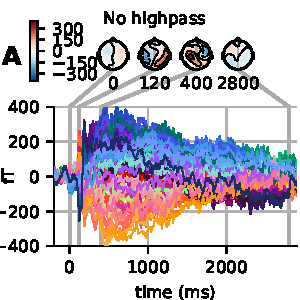
\includegraphics[width=0.31\linewidth]{figures/FanningA.pdf}
  \hspace{0.5em}
  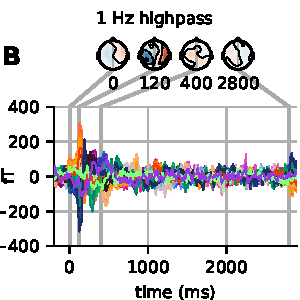
\includegraphics[width=0.31\linewidth]{figures/FanningB.pdf}
  \hspace{0.5em}
  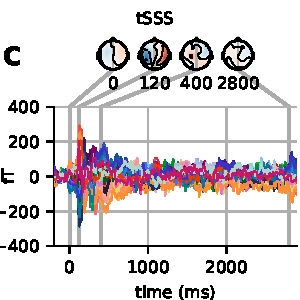
\includegraphics[width=0.31\linewidth]{figures/FanningC.pdf}
\caption[Comparison of highpass filtering and tSSS on evoked response.]{(A) Evoked response in magnetometers for subject 3 with baseline correction. Note how signals tend toward the baseline late in the epochs (where the rightmost time point, 2.9 sec, is the earliest possible start time for the next stimulus). (B) The highpass filtered version of the signal and (C) the signal processed with temporal SSS (tSSS). Both reduce the magnitude of the slow and late sustained responses shown in (A).}
\label{fig:fanning}
\end{figure}
  
It is common practice to use baseline correction so that any constant offsets in the baseline are removed. High-pass filtering achieves similar results by eliminating the low-frequency components in the data. However, when using baseline correction, the low frequency drifts present in the data are not attenuated. Thus it is useful to examine long time-courses of the data, if possible, to determine if low-frequency drifts are present. The difference between the two approaches can be seen in Figure~\ref{fig:fanning}. The evoked responses in the figure are across-trial averages for the famous face condition. If a maximum time of approximately one second were used, a simple baseline correction would appear to produce an undesired \textit{``fanning"} in the later responses. Indeed one can observe in Figure~\ref{fig:fanning}A that at one second post-stimulus, the channels still significantly deviate from zero. However, by extending the time window much longer (here to 2.9 seconds) we can see that the signals do mostly return to the baseline level.

\emph{Caveats and Alternatives} With highpass filter at 1\,Hz (and 1 Hz transition band), the signal returns to the baseline level much sooner. Note also the similarities between Figures~\ref{fig:fanning}B and~\ref{fig:fanning}C, illustrating how using temporal version of the SSS algorithm (tSSS) acts implicitly as a high-pass filter. For tSSS, we use a buffer size of length 1\,s and a correlation limit of 0.95 to reject overlapping inner/outer signals. However, these high-passing effects come at the expense of distorting the sustained responses. We will thus focus on analyses that utilize the baseline-corrected data here.

\section{Sensor space analysis}
An important step in analyzing data at single-subject and group levels is sensor-space analysis. Here we show how several different techniques can be employed to understand the data.

\begin{figure}[t]
  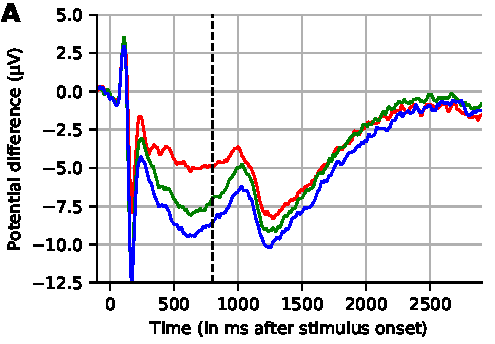
\includegraphics[width=0.49\linewidth]{figures/grand_average_highpass-NoneHz.pdf}
  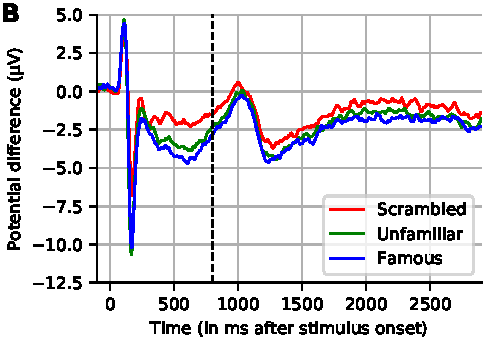
\includegraphics[width=0.49\linewidth]{figures/grand_average_highpass-1Hz.pdf}
\caption[Grand averaged evoked response across 16 subjects.]{Grand averaged evoked response across 16 subjects for channel EEG065.
(A) No highpass filter. (B) Highpass filtered at 1.0 Hz. Note that, similar to (A), the results reported by \cite{wakeman2015multi} (dashed line at 800 ms indicates where their plot stopped) show large drifts, but these return to near-baseline levels toward the end of a sufficiently long interval (here, 2.9 seconds) even without applying a highpass filter.}
\label{fig:grand_average}
\end{figure}  

\subsection{Group average}

A classical step in group studies is known as ``grand averaging''~\citep{delorme-etal:15}. It is particularly common for EEG studies and it consists in averaging ERPs across all subjects in the study. As not all subjects have generally the same good channels, this step is commonly preceded by an interpolation step to make sure data are available for all channels and for all subjects. Note that grand averaging is more common for EEG than for MEG, as MEG tends to produce more spatially resolved topographies that may not survive averaging due to signal cancellations.

The grand average of the 16 subjects for one EEG sensor (EEG065) is presented in Figure~\ref{fig:grand_average}. We selected this channel to compare with the figure proposed by \cite{wakeman2015multi}. We present the grand average for the `scrambled', `famous', and `unfamiliar' conditions using a high-pass filter (cf. Section~\ref{sec:baseline}), and baseline corrected using prestimulus data. This figure replicates the results in \citep{wakeman2015multi}. We can see the early difference between faces, familiar or unfamiliar, and scrambled faces around 170\,ms. We can also notice a difference in the late responses between the two conditions `unfamiliar' and `famous'. However, the effect is smaller when using high-pass filtering, as it corrects for the slow drifts.

\emph{Caveats} For MEG, the grand average may wash out effects or induce spurious patterns due to misalignment between head positions. SSS can be used to align subjects in one common coordinate systems.
    
\subsection{Contrasting conditions}

Two conditions of interest are often compared using a statistical contrast. A paired contrast between two conditions can be computed by computing the difference in their evoked responses. The difference does not take into account the number of trials used to compute the evoked response -- in other words, each condition is weighted equally. Recall that the event IDs were organized hierarchically during epoching (as described in Section~\ref{sec:epoching}). Such a hierarchical organization is natural for contrasting conditions in the experiment, as we compare not only `faces' against `scrambled faces', but also `famous faces' against `unfamiliar faces'.
    
\emph{Caveats.} Although this is standard in EEG pipelines, historically, for computing the source estimates, weighted averages have sometimes been used. However, MNE provides a mathematically correct estimate for the effective number of trials averaged, so equal-weighted combinations (additions or subtractions) of evoked data are properly accounted for even in the context of unequal trial counts. This logic, however, does not apply when working with experimental protocols (for example, oddball tasks) which, by design, produce many more examples of one than the other conditions.

\subsection{Cluster statistics}

\begin{figure}
\centering
    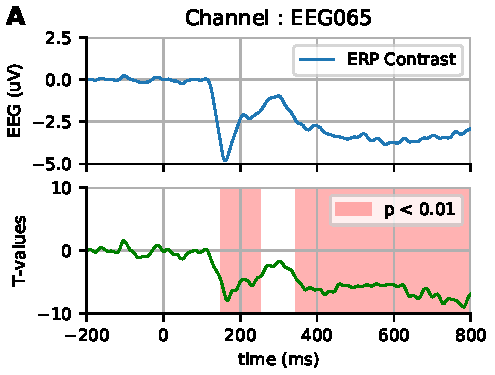
\includegraphics[width=0.49\linewidth]{figures/sensorstat_highpass-NoneHz.pdf}
    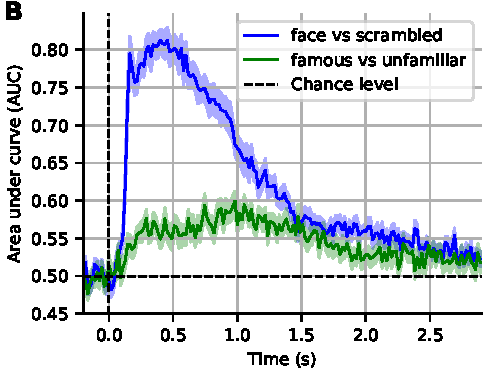
\includegraphics[width=0.49\linewidth]{figures/time_decoding_highpass-NoneHz.pdf}
    \caption[Sensor space statistics.]{Sensor space statistics. (A) A single sensor (EEG065) with temporal clustering statistics. The clustering is based on selecting consecutive time samples that have exceeded the initial paired t-test threshold (0.001), and finding clusters that exceed the size expected by chance according to exchangability under the null hypothesis ($p < 0.01$, shaded areas). (C) Cross-validation score of time-by-time decoding. As opposed to a cluster statistic, time decoding is a multivariate method which pools together the signal from different sensors to find discriminative time points between two conditions.}
\label{fig:fig_sensorstat}
\end{figure}

To contrast our conditions of interest, here we use a non-parametric clustering statistical procedure as described by \cite{maris_nonparametric_2007}. This combines neighboring values that are likely to be correlated (here, neighboring time instants) to reduce the problem of multiple comparisons. The contrast score (here the  t-values) for each cluster are summed up to compute the mass of each cluster, which serves as our actual statistic. Next, we need to know if the distribution data in our two conditions (here measured using cluster sizes) is significantly different from what would be obtained by chance. For this purpose, we generate a null distribution from the data by randomly swapping our conditions for each subject according to exchangability under our null hypothesis. In this case, it is equivalent to changing the sign of the contrast data (as we are using a one-sample t-test on the difference between conditions), and then recomputing the maximal cluster size for each permutation. From an estimate of the distribution of the maximum cluster size under the null-hypothesis, we can compute the probability of observing each cluster relative to this distribution. This gives us a control of the \ac{FWER}, a.k.a. type 1 error, when reporting a significant difference between the distribution of data in our two conditions.

Running this nonparametric permutation test on the single sensor EEG065 (also used by \cite{wakeman2015multi}) revealed two across-time clusters that allowed us to reject the null hypothesis at the level $p < 0.01$. To perform the clustering, we used an initial thresholding of $p < 0.001$ with a two-sided paired t-test (Figure~\ref{fig:fig_sensorstat}). The statistic used was a one-sample t-test on the contrast ERPs using as contrast weights (0.5 for 'familiar', 0.5 for 'unfamiliar' and -1 for 'scrambled'), testing for the condition faces versus scrambled faces. A first cluster appears around the same time as the evoked response, and the other captures the late effects. Running another statistical test, this time incorporating the spatial distribution of the sensors into the clustering procedure, yields one spatiotemporal cluster with $p < 0.05$ for the contrast condition as shown in Figure~\ref{fig:stclusterstats}.

\begin{figure}
\centering
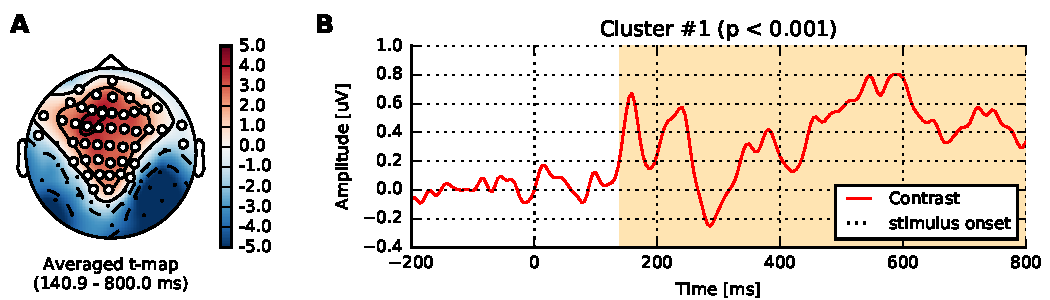
\includegraphics[width=\linewidth]{figures/spatiotemporal_stats_cluster_highpass-NoneHz-00.pdf}
\caption[Spatiotemporal cluster statistics on EEG sensors.]{Spatiotemporal cluster statistics on the EEG sensors. (A) Topographic map of the t-statistic. (B) Average over the sensors that were part of the significant cluster.}
\label{fig:stclusterstats}
\end{figure}
\emph{Alternatives and caveats.} It is important to note that this clustering permutation test does not provide feature-wise (vertex, sensor, time point, etc.) but \emph{cluster-level} inference. This is because the test statistic is the cluster size and not any specific t-values used to obtain the cluster in the first place. When inspecting a significant cluster, no conclusion can be drawn on which time point or location was more important. A computationally more expensive alternative is the so-called TFCE method which provides feature-level inference and, moreover, mitigates the problem of having to set the initial threshold on the t-values to define clusters~\citep{TFCE}. When strong \emph{a priori} hypotheses exist considering few regions of interest in either time, frequency or space can be a viable alternative. In that case, the multiple comparisons problem may be readily alleviated by more conventional measures, such as \acp{FDR} \citep{FDR}.

\subsection{Time Decoding}

As an alternative to mass-univariate analysis, a event-related brain dynamics can studied using a multivariate decoding approach~\citep{ramkumar2013feature,king2014characterizing}. Here, a pattern classifier, often a linear model (e.g. logistic regression) is trained to discriminate between two conditions: `face' versus `scrambled', and also `famous faces' versus `unfamiliar faces'. The classifier can be trained on single trials, time-point by time-point. The prediction success can then be assessed with cross-validation at every instant, yielding an intuitive display of the temporal evolution of discrimination success. In Figure~\ref{fig:fig_sensorstat}B, we display such cross-validation time-series averaged across the 16 subjects. As anticipated, discriminating between faces and scrambled faces is much easier than discriminating between `famous' and `unfamiliar' faces, based on information in early components in the first second after stimulus-onset.

For performance evaluation, we use is area under the receiver operating characteristic curve (ROC-AUC), as it is a metric that is insensitive to class imbalance (i.e., differing numbers of trials) therefore allowing us to average across subjects, and also to compare the two classification problems (faces vs. scrambled and familiar vs. unfamiliar). Results on the faces vs. scrambled conditions show that time-resolved decoding reveals decoding accuracy greater than chance around the same time intervals as the non-parametric cluster statistic. The effect although appears here quite sustained over time. Results on familiar \emph{vs.} unfamiliar conditions are also above chance from 200 to 300\,ms, however the best decoding performance emerges later for this contrast. This more subtle effect even peaks after 800\,ms, which exceeds the time window investigated in the original study.

\section{Source reconstruction}

\begin{figure}
\centering 
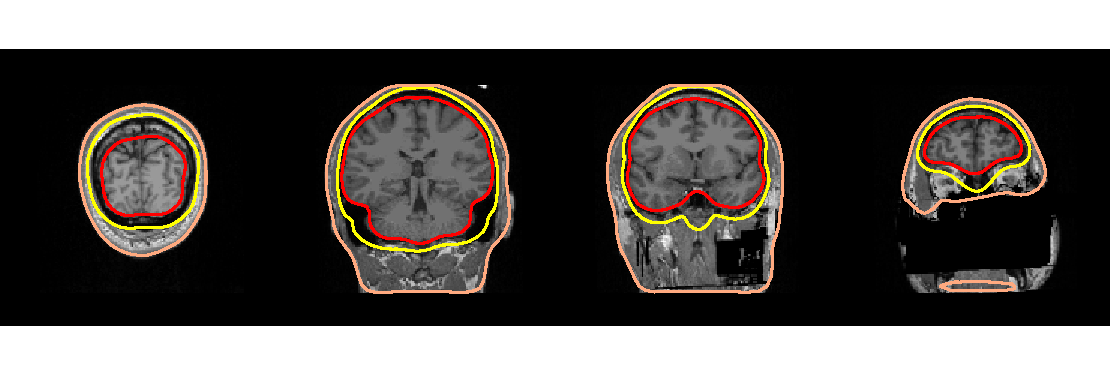
\includegraphics[width=\linewidth]{figures/sub001_bem.pdf}
\caption[BEM surfaces on flash MRI images.]{BEM surfaces on flash MRI images. The inner skull, outer skull and outer skin are outlined in color.}
\label{fig:fig_bem}
\end{figure}

The MNE software relies on the FreeSurfer package~\citep{dale-fischl-etal:99,fischl-serena-etal:99} for the processing of anatomical MRI images. This automatic procedure is run using the command \code{recon-all} on the T1 MRI of each subject. This provides many useful pieces of information, but the most critical here are the cortical reconstruction (a high resolution triangulation of the interface between the white and the gray matter) and the inner skull surface.

For inverse source reconstruction and beamforming, we must first compute the forward solution, often called a gain or lead field matrix. It describes the sensitivity of the sensors to a given set of dipoles~\citep{mosher-leahy-etal:99}. Computing the gain matrix, which is a linear operator, requires having a so-called source space of dipole locations, a conductor model for the head, and the sensor locations relative to those dipoles. This latter requirement in practice means putting in the same coordinate system the MRI (where the source space and conductor model are defined), the head (where the EEG electrode locations are recorded or digitized), and the MEG device (where the MEG sensors are defined). This step is commonly referred to as \emph{coregistration}. We will cover each of these steps below.

\subsection{Source space}
As we expect most of our activations of interest to be due to cortical currents~\citep{dspm}, we position the candidate dipoles on the cortical mantle. We chose a source space obtained by recursively subdividing the faces of an octahedron six times (oct6) for both the left and right hemispheres. This leads, for each subject, to a total of 8196 dipoles evenly spaced on the cortical surface (See Figure 6 in \citep{mne}).

\subsection{Head conductivity model}
MNE can use simple spherical conductor models but when the MRI of subjects are available, the recommended approach is to use a piecewise-constant conductivity model of the head. Tissue conductivities are defined for each region inside and between the segmented interfaces forming the inner skull, outer skull and the outer skin. It corresponds to a so-called three layer model, however a single layer is possible when using only MEG data. The default electrical conductivities used by MNE are 0.3 S/m for the brain and the scalp, and 0.006 S/m for the skull, i.e., the conductivity of the skull is assumed to be 1/50 of that of the brain and the scalp. With such a head model, Maxwell equations are solved with a \ac{BEM}.

In addition to the T1 MRI image, \ac{FLASH} images are provided in the present dataset. Such MRI images allow to automatically extract precise surfaces for the inner skull and outer skull. Note that in the absence of FLASH images, MNE offers a somewhat less accurate solution based on the watershed algorithm. One output of the MNE automatic BEM surface extraction is presented in Figure~\ref{fig:fig_bem}. It contains the three surfaces needed for the computation of the EEG gain matrix. In our results shown here, we used only the MEG data for source reconstruction, and consequently only made use of the inner skull surface in a one-layer model. As MRIs shared here are defaced, outer skull and scalp surfaces are anyway quite wrong, so we considered it satisfactory to only use the inner skull surface.

Quality insurance at this stage consists in checking that the three surfaces do not intersect with each other and that they follow the interfaces between the brain, the skull and the skin. A slice-by-slice visual inspection of approximate alignment is best and is conveniently proposed by MNE BEM plotting function that outputs a figure as presented in Figure~\ref{fig:fig_bem}.

Here, as the MRIs shared in this dataset were anonymized, the outer skin surface obtained automatically using Freesurfer intersected with the outer skull surface for most subjects. However this is  rarely observed with non defaced T1 MRI images.

\subsection{Coregistration}
In order to compute the gain matrix, the sensor locations (and normals), head model, and source space must be defined in the same coordinate system. In practice, this means that the BEM surfaces and source space (which are defined in MRI coordinates) must be coregistered with the EEG sensors, which are digitized in the Neuromag head coordinate frame (defined by the digitized nasion, LPA, and RPA). The MEG sensor locations and normals are defined in the MEG device coordinate frame. Typically, the MEG-to-head transformation is determined during acquisition using head position indicator (HPI) coils (or redefined using head position transformation using Maxwell filtering), so MEG sensor locations can be easily transformed to head coordinates. The transformation between the MRI and head coordinate frames is typically estimated by identifying corresponding points in the head and MRI coordinate systems, and then aligning them.

The most common points used to provide an initial alignment are the fiducial landmarks that define the Neuromag head coordinate frame. They consist of the nasion and two pre-auricular points which are digitized during acquisition, and are then also identified by offline visual inspection on the MRI images. Additional digitization points on the head surface can also be used to better adjust the coregistration. In this study, on average, 135 digitization points were available per subject. The transformation, which consists of a rotation matrix and a translation vector, is then typically saved to a small file, also called \emph{trans} file, and later used to compute the forward solution.

For quality insurance, MNE offers a simple function to visualize the result of the coregistration.
Figure~\ref{fig:fig_trans} shows one example obtained with this function with the defaced, low-resolution MRI head surface. As here the MRI were defaced, many important digitization points close to the nose where useless. To reduce the risk of bad coregistration due to defaced MRI images, we used the trans files kindly provided by the original authors.
    
\begin{figure}
\centering
    
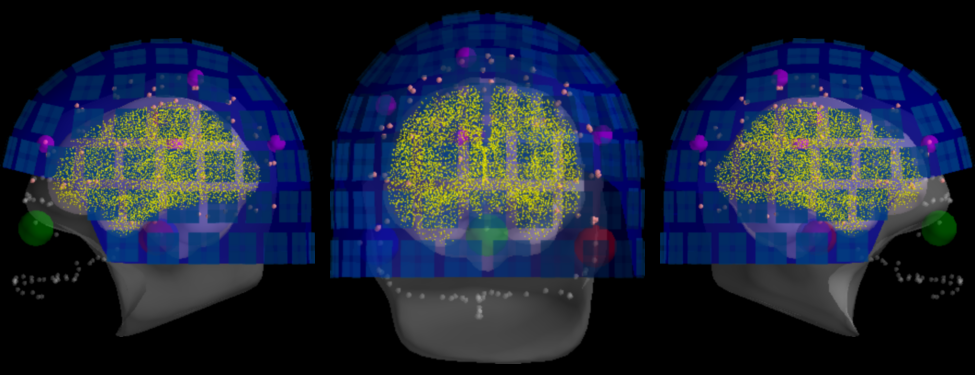
\includegraphics[width=\linewidth]{figures/sub001_alignment.pdf}
 \caption[Visualization of coregistration quality]{The result of head-to-MRI (and MEG-to-head) transformations with inner skull and outer skin surfaces for one subject. Note that the MEG helmet is well aligned with the digitization points. The digitized fiducial points are shown with large dots, EEG electrodes with small pink dots, and extra head digitization points with small gray dots. Note that the anonymization of the MRI produces a mismatch between digitized points and outer skin surface at the front of the head.}
\label{fig:fig_trans}
\end{figure}

\subsection{Covariance estimation and Whitening}

As inverse solvers typically assume Gaussian noise distribution on the sensors with an identity covariance matrix, a whitening step is first necessary~\citep{engemann2015automated}. M/EEG signals are indeed highly spatially correlated. Whitening also allows integration of data from different channel types that can have different units and signal amplitudes which differ by orders of magnitudes (cf. planar gradiometers, axial magnetometers, and EEG electrodes).
To whiten the data, one must provide an estimate of the spatial noise covariance matrix. This can be computed from empty-room recordings for MEG or pre-stimulus periods~\citep{mne}. Here, we followed the approach proposed by~\citet{engemann2015automated}, which consists in picking the best model and estimating the best regularization parameters by computing the Gaussian log-likelihood of left-out data (i.e., a cross-validation procedure). Such an approach has been shown to be particularly robust for scenarios where a limited number of samples is available for covariance estimation.

In this analysis, the noise covariance is estimated from the 200\,ms of data before stimulus presentation. During this period, only a fixation color is visible at the center of the screen. Given this covariance matrix and the gain matrix, one can assemble the inverse operator to compute the MNE or \ac{dSPM} solutions~\citep{dspm}.

The quality of the covariance estimation and whitening can have a significant impact on the source localization results. The rank-adjusted \ac{GFP} has been proposed by \citet{engemann2015automated} as a measure that can be used to check the quality of the whitening. It is defined as GFP$=\sum_i x^2_{i} / P$ where $P$ is the rank of the data and $x_i$ is the signal in the $i$th sensor at a time instant. The GFP being a normalized sum of Gaussian random variables with an identity covariance matrix, it follows a $\chi^2$ distribution with an expected value of 1. What is not captured by our noise model, e.g. actual brain signals, thereof will pop out in the whitened domain.
To understand this better, we show some whitened data and the GFP in Figure~\ref{fig:plot_white}. If the Gaussian assumption has not been violated, we expect the whitened data to contain 95\% of the signal within the range of -1.96 and 1.96, which we mark in dotted red lines. The baseline period, where we estimated our noise covariance from, appears to satisfy this assumption. Consequently, the GFP is also 1 during this period. One can observe a strong increase in the GFP just after the stimulus onset, and that it returns slowly to 1 at the end of the time interval. Such a diagnostic plot can in fact be considered essential for quality assurance before computing source estimates. This has as consequence that what appears in the source estimates depends on our noise model. For instance, using a noise covariance obtained from empty room recordings would suggest the presence of ``interesting'' signals, simply because it contains brain signals that are fundamentally different from the empty room noise.

For the LCMV beamformer, we also need to estimate a signal covariance. For this we use the 30\,ms to 300\,ms window after the stimulus onset. The data covariance is again regularized automatically following~\citep{engemann2015automated} and is motivated by the results from~\citep{Woolrich:2011,MindTheCov}.

\begin{figure}
\centering
 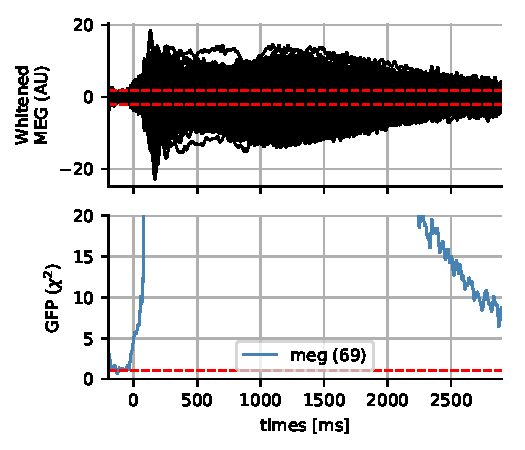
\includegraphics{figures/sub004_highpass-NoneHz-plot_white_meg.pdf}
\caption[Whitened MEG data at the evoked level for one subject]{Whitened MEG data for subject 4 and the global field power (GFP) which follows a $\chi^2$ distribution if the data is assumed Gaussian. The dotted horizontal red lines represent the expected GFP during the baseline for Gaussian data. Here the data slowly return to baseline at the end of the epoch.}
\label{fig:plot_white}
\end{figure}

\emph{Caveats.} If empty-room data are used to whiten processed signals, one must make sure that the obtained noise covariance matrix corresponds to the processed data rather than to the original empty-room data. This is done by processing the empty-room data with exactly the same algorithm and the same parameters as the actual data to be analyzed. For example if SSS, SSP or ICA are applied on processed data, it should be applied to empty room data before estimating the noise covariance. Concretely, SSP vectors and ICA components projected out from the data of interest should also be projected out from the empty room data. SSS should be performed with identical parameters.
Also note that magnetometers and gradiometers are whitened jointly. Moreover, if SSS was applied, the display of whitening treats magnetometers and gradiometers as one channel-type. For proper assessment of whitening, a correct assessment of the spatial degrees of freedom is necessary. The number of SSS dimensions is commonly a good estimate for the degrees of freedom. When movement compensation was applied, the estimated data rank may be unreliable and suggest too many independent dimensions in the data. 
Even the actual number of SSS components can be misleading in such circumstances. It is then advisable to inspect the eigenvalue spectrum of the covariance matrix manually and specify the degrees of freedom manually using the rank parameter.

\subsection{Inverse solvers and beamforming}
% Given the gain matrix $\mathbf{G}$, our data can be expressed as:
% \begin{equation}
% \mathbf{M} = \mathbf{GX} + \mathcal{P}(\mathbf{X)}
% \end{equation}
% where $\mathbf{M}$ is the sensor-space data, $\mathbf{G}$ is the gain matrix and $\mathbf{X}$ is the source time course. Often, a penalty term $\mathcal{P}(\mathbf{X)}$ is also applied to inject certain constraints on the data, such as sparsity or smoothness.

The goal of an inverse solver is to estimate the locations and the time courses of the sources that have produced the data. While the data $\mathbf{M}$ can be expressed linearly from the sources $\mathbf{X}$ given the gain matrix $\mathbf{G}$, $\mathbf{M} \approx \mathbf{GX}$, the problem is ill-posed. Indeed $\mathbf{G}$ has many more columns than rows. This means that there are more unknown variables (brain sources) than the number of measured values (M/EEG sensors) at each time point. This also implies that the solution of the inverse problem is not unique.

For this reason, many inverse solvers have been proposed in the past ranging from dipole fits~\citep{scherg-etal:85,mosher-lewis-etal92}, \acp{MNE}~\citep{Hamalainen:1984}, and scanning methods such as RAP-MUSIC or beamformers such as LCMV and DICS \citep{Van_Veen:1997,gross-etal:2001,Sekihara:2005}. There is therefore no absolute perfect inverse solver, although some are more adapted than others depending on the data. Some are adapted to evoked data for which one can assume a few set of focal sources. Some also give you source amplitudes in a proper unit, which is nAm for electrical current dipoles, such as MNE, MxNE~\cite{gramfort-etal:2013} or dipole fits. Some give spatially normalized statistical maps such as dSPM~\citep{dale2000dspm} or LCMV combined with neural activation index (NAI) filter normalization~\citep{Van_Veen:1997}.

Given the important usage of dSPM and the LCMV beamformer in the cognitive neuroscience literature, we wanted to investigate how much using one of these two most commonly used methods was affecting the source localization results. The dSPM solution was computed with MNE default values: loose orientation of 0.2, depth weighting~\citep{lin2006assessing} of 0.8, and SNR value of 3. The LCMV used was a vector beamformer with unit-noise-gain normalization~\citep{Sekihara:2005} as implemented in MNE 0.15. No specific regularization was used in the beamformer filter estimation.

% \subsubsection{Dynamic Statistical Parameter Mapping (dSPM)}

% dSPM~\citep{dale2000dspm} is similar to Minimum Norm Estimates (MNE) but produces a statistical map of where the activity is different from background noise. In that sense, the dSPM source activations do not have a physical unit. The consequence of this normalization is that it removes the bias towards superficial sources that is present in MNE. The inverse solver produces a spatiotemporal estimate but in Figure~\ref{fig:fig_stc}, we visualize the spatial activations in only a single time point of interest. The source estimates are visualized by smoothing the data to fit the vertices in the tessellation of the cortical surface (Figure~\ref{fig:fig_stc}). In MNE, \emph{smoothing} is an iterative process which blurs the data to the surface.
 
% \subsubsection{Linearly Constrained Minimum Variance (LCMV) beamforming}

% LCMV is a spatial filter used to estimate the sources. The filter works by passing the activity at a certain location while attenuating the noise from other locations. It requires only that the sources are uncorrelated. It tends to give more focal activation maps compared to conventional source localization methods~\citep{vanveen-etal:1997}. This is what we observe also in our experiments in Figure~\ref{fig:fig_stc}.

% It is however not always clear if the sources are correlated or not. If they are, LCMV results can lead to large errors in the source estimates \citep{vanveen-etal:1997,hansen2010meg}.
\subsection{Group source reconstruction}

\begin{figure}
\centering
\begin{minipage}{0.4\linewidth}
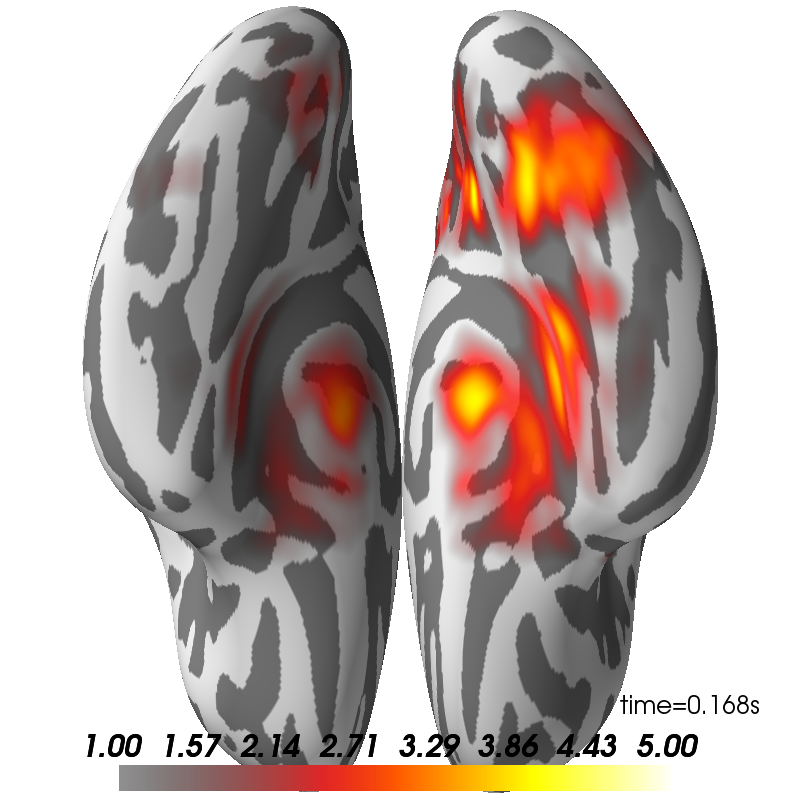
\includegraphics[width=\linewidth]{figures/dspm-ave_highpass-NoneHz.png}
\end{minipage}
\begin{minipage}{0.4\linewidth}
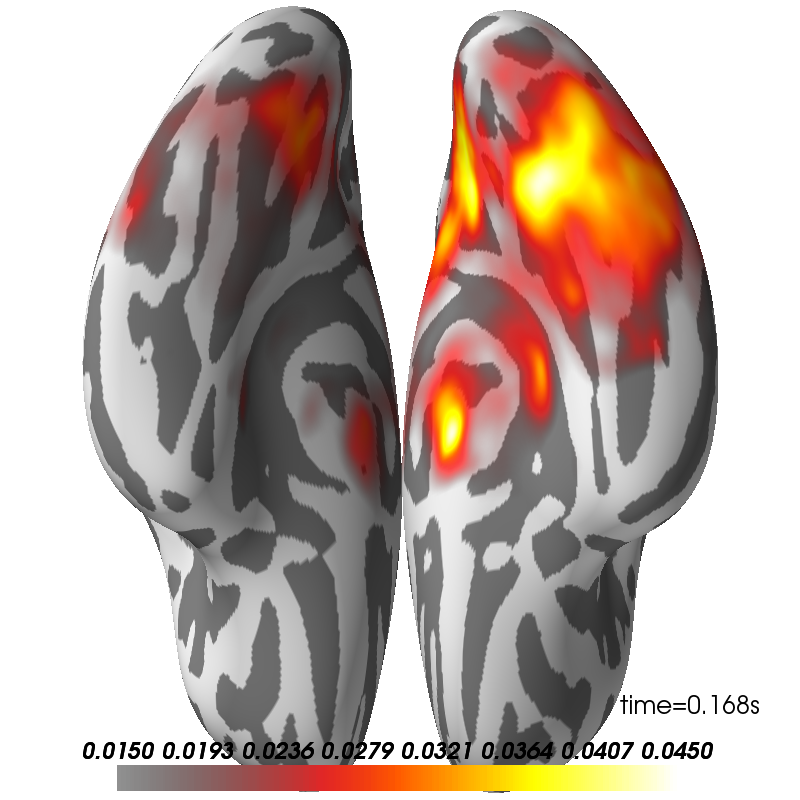
\includegraphics[width=\linewidth]{figures/lcmv-ave_highpass-NoneHz.png}
\end{minipage}
\caption[Group average on source reconstruction with dSPM and LCMV.]{Group average on source reconstruction with dSPM (left) and LCMV (right). Here, we have the ventral view of an inflated surface with the anterior-posterior line going from the bottom to top of the image. Right hemisphere is on the right side.}
\label{fig:fig_stc}
\end{figure}

To analyze data at the group level, some form of data normalization is necessary, whereby data from all subjects is transformed to a common space in a manner that helps compensate for inter-subject differences. This procedure, called \emph{morphing} by the MNE software, exploits the FreeSurfer spherical coordinate system defined for each hemisphere~\citep{dale-fischl-etal:99,fischl-serena-etal:99}. In our analysis, the data are morphed to the standard FreeSurfer average subject named \code{fsaverage}. The morphing procedure is performed in three steps. First, the subsampled data defined on the high resolution surface are spread to neighboring vertices using an isotropic diffusion process. Next, registration is used to interpolate the data on the average surface. And finally, the data defined on the average surface is subsampled to yield the same number of source locations in all subjects (here, 10242 locations per hemisphere). Once the morphing is complete, the data is simply averaged.

What is presented in Figure~\ref{fig:fig_stc} is the group average of the dSPM and LCMV beamformer solutions on contrast between faces and scrambled
at 170\,ms post-stimulus.

Looking at these results, one can observe that both methods highlight a peak of activation on the right ventral visual cortex known to be involved in face processing~\citep{grill2017functional,grill2004fusiform,wakeman2015multi}. The dSPM peak seems however to be slightly more anterior.

\subsection{Source-space statistics}

\begin{figure}
\centering
\begin{minipage}{0.5\linewidth}
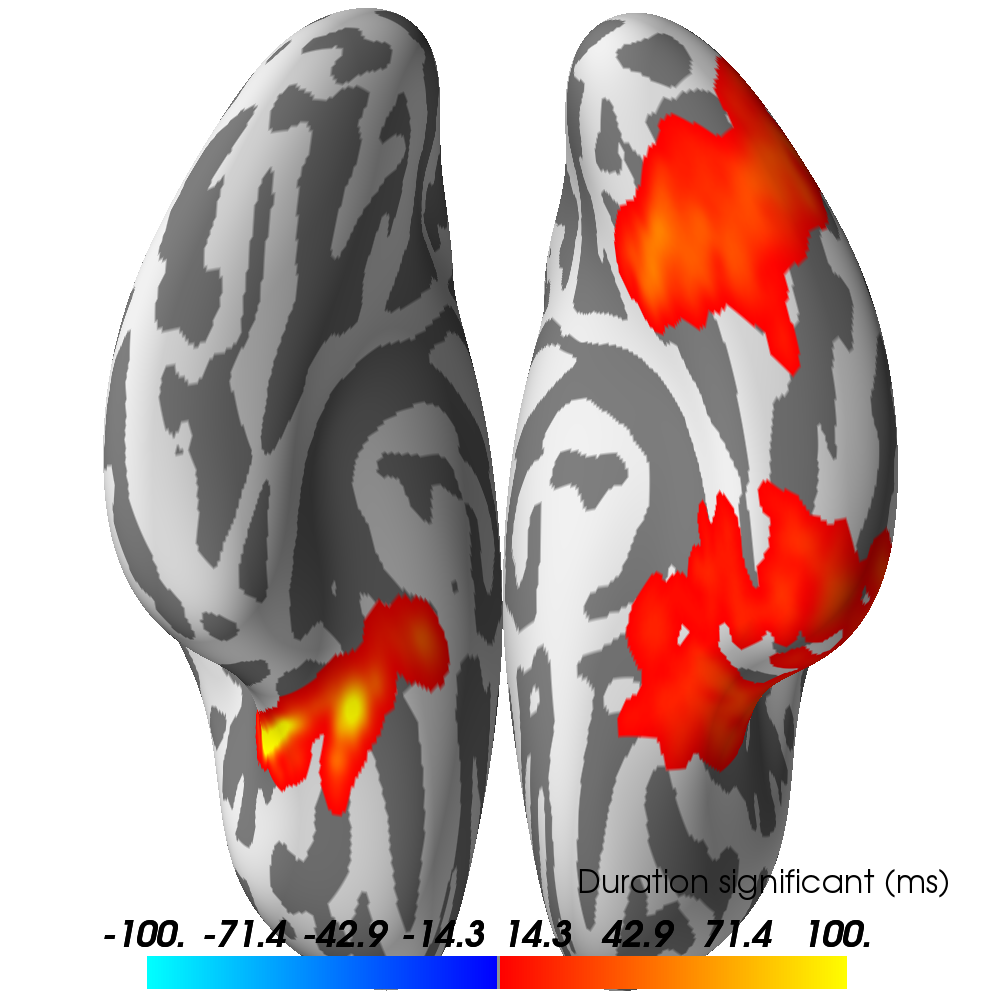
\includegraphics[width=\linewidth]{figures/source_stats_highpass-NoneHz.png}
\end{minipage}
\caption[Spatio-temporal source space clusters obtained by nonparametric permutation test.]{Spatio-temporal source space clusters obtained by nonparametric permutation test that allowed rejection of the null hypothesis that the distribution of data for the "faces" condition was the same as that of "scrambled". The clusters here are collapsed across time such that vertex colors indicate the duration that each vertex was included in its cluster (each cluster here occurring with type I error corrected $p < 0.05$). Hot colors indicate durations for vertices in clusters where response for faces $>$ scrambled (cool colors would be used for scrambled $>$ faces, but no such clusters were found).}
\label{fig:fig_source_stats}
\end{figure}

Just as we did for the sensor time courses, we can subject the source time courses (here for dSPM only) to a cluster-based permutation test. The null hypothesis is again that there is no significant difference between the data distributions (here measured using cluster size) for faces versus scrambled (paired). Under each permutation, we do a paired t-test across subjects for the difference between the (absolute value of the) faces and scrambled values for each source space vertex and time point. These are clustered, and maximal cluster size for each permutation is selected to form the null distribution. Cluster sizes from the actual data are compared to this null; in this case we find three clusters that lead us to reject the null with $p < 0.05$ (see Figure~\ref{fig:fig_source_stats}).
 
 \emph{Alternatives} When strong hypotheses exist with regard to spatial, temporal and spectral regions of interest, it may be preferable to test the experimental hypotheses on fewer well-chosen signals. In the context of a group analysis, a linear multilevel modeling approach may provide an interesting option for obtaining joint inference at the single subject and group level~\cite{gelman2006multilevel,baayen2008mixed}.
 
% \begin{figure}[htbp]
%     \centering
%         \includegraphics[width=\linewidth]{morphing.jpg}
%     \caption{Current estimates obtained from an individual subject can be remapped (morphed),
%     {\em i.e.}, normalized, to another cortical surface, such as that of the FreeSurfer average brain ``\emph{fsaverage}''
%     shown here. The normalization is done separably for both hemispheres using a non-linear registration
%     procedure defined on the sphere~\citep{dale-fischl-etal:99,fischl-serena-etal:99}.
%     Here, the N100m auditory evoked response is localized usin g dSPM and then mapped to
%     ``fsaverage''. \REV{Images were produced with {\em PySurfer}.}}
%     \label{fig:morphing}
% \end{figure}

\section{Discussion and conclusion}
\label{sec:group_study_discussion}
% Summarize intention and results of the study and goals.
Analyzing M/EEG requires successive operations and transformations on the data. At each analysis stage, the different processing choices can affect the final result in different ways. While this situation encourages tailoring data analysis strategies to the specific demands of the scientific problem, this flexibility comes at a cost and can lead to spurious findings when not handled appropriately~\citep{ioannidis2005,simmons2011false,Carp2012}.
% Indeed, the intrinsic noise of psychological measurements combined with the flexibility of data analysis in neuroimaging and its perennially small sample sizes may suggest a particularly aggravated replication crisis in cognitive neuroscience compared to medical research and psychology~\citep{szucs2017}.
In the absence of fully automated data analysis pipelines that can optimize the choice of processing steps and parameters, it is crucial to develop principled approaches to planning, conducting and evaluating M/EEG data analysis.

The present study makes the effort to elucidate common elements and pitfalls of M/EEG analysis. It presents a fully reproducible group analysis of the publicly available dataset from~\cite{wakeman2015multi}.
All code and results are publicly accessible \url{http://mne-tools.github.io/mne-biomag-group-demo/}. The study provides contextualized in-depth discussion of all major steps of the analysis with regard to alternative options, caveats and quality control measures. As a rare contribution to the M/EEG literature, this study illustrates in comparative figures, the experimental results obtained when changing essential options at different steps in the analysis. In the following, we want to share some insights that we obtained from working together on this study. 

% 1) Lessons learned from this project: collaborative data analysis
\emph{Collaborative data analysis}. In our experience, high-level planning and hands-on data analysis are commonly divided between, e.g., masters or doctoral students, post-docs, and senior researchers. As a consequence, the results are typically appreciated from figures produced without connection to the research code that generated them. In this study, several authors contributed repeatedly to the code, analyses were repeated on different computers, and results were inspected in an ongoing fashion by many authors. This experience has had as consequence that incoherences, model violations, and other quality concerns were perhaps detected more often than usual, which has greatly contributed to the overall quality of the data analysis. While it is perhaps too extreme or onerous to recommend adopting social interaction habits from open source software development---such as peer review, pair or extreme programming---in scientific data analysis, we believe that data analysis should not be done in isolation. In order to enable full-blown collaborative data analysis in research, analysis must be repeatable, hence, scripted, and a minimum of code organization and readability must be enforced. On the other hand, the best coding efforts will have limited impact if there are not multiple authors with fresh and active data analysis habits. We hope that the example stated by this paper, together with the open source tools and the community it is built upon, can stimulate more collaborative approaches in M/EEG research.

% 2) Lessons learned from this project: The costs of reproducibility
\emph{The costs of reproducibility}. It is a commonly neglected reality that reproducibility comes at a price. Making an analysis strictly reproducible not only requires intensified social interactions, hence more time, but also demands more computational resources. It is a combinatorially hard problem if one were to consider all the potential sources of variability. For example, analyses have to be repeated on different computers with different architectures and performance resources. This sometimes reveals differences in results depending on the hardware, operating system, and software packages used. As observed in the past by \cite{glatard-etal:15}, we noticed that some steps in our pipeline such as ICA are more sensitive to these changes, eventually leading to small differences at the end of the pipeline, which is in our case are cluster-level statistics in the source space. Of course, differences due to these changes are harder to control and enforce in the context of today's fast technological progress. Indeed, what we manage to achieve is reproducibility, as opposed to the pure replicability which would be the case if the same results could be achieved even when the computer hardware and software packages were changed.

Also, when code is developed on large desktop computers which are common in many laboratory settings, replication efforts with lower-performance workstations may incur high costs in terms of human processing time. The analysis not only runs slower but may crash, for example due to differences in computer memory resources. We therefore emphasize the responsibility of software developers in providing scalable performance control and the responsibility of hands-on data analysts to design the analysis bearing performance and social constraints in mind. In other words, consider that code needs to run on someone else's computer.


% 3) Lessons learned from this project: when to stop. 
\emph{When to stop?} Obviously, in the light of the current replication crisis, clear rules need to be established on when to stop improving the data analysis~\citep{simmons2011false,szucs2017}. A particular risk is emanating from the possibility of modifying the analysis code to eventually confirm the preferred hypothesis. This would invalidate inference by not acknowledging all the analysis options explored. Apart from commonly recommended preregistration practices and clean hold out data systems, we want to emphasize the importance of quality criteria for developing the analysis. The bulk of M/EEG preprocessing tasks are either implicitly or explicitly model-based, as shown by the rich battery of quality control visualizations presented in this chapter. Such plots allow to assess if M/EEG analysis outputs can be considered good signals. Consequently, analysis should be stopped when no further improvement on quality control metrics is to be expected, within a reasonable time investment. In other words, not research hypotheses (and statistical significance of results) but rather signal quality metrics are the criterion for constructing M/EEG analyses. Ideally, only when quality control is done, should the contrast(s) of interest be investigated.

%XXX OLD TEXT XXX
% XXX I have no idea what is the goal of this section. It seems just a bit redundant. As a reader I feel bored because I cannot smell the direction and I feel like listening to monologue of someone talking. 
% In the preceding sections, we have first detailed the preprocessing steps, including filtering, bad segment detection, artifacts correction, epoching, averaging, source reconstruction, and finally statistics. Visually inspecting individual-channel PSD is easy to do and allows for a preliminary screening of bad channels and potentially strong transient artifacts. As obvious as it may seem, visually inspecting the evoked sensor space data is mandatory and MNE offers convenient routines to visualize topographies and so-called butterfly plots, which overlay evoked potentials for each sensor with lines color-coded by sensor locations. It facilitates easily spotting the remaining eye blink artifacts that affect primarily frontal sensors. Inspecting the butterfly plots for transient artifacts can be useful even for resting state data despite having no evoked response. While MNE offers automated methods to detect bad ICA components, it can sometimes fail and visual inspection of the ICA sources is always a good idea. In terms of source localization, MNE offers the possibility to visualize whitened data to better assess what sources to expect in the brain, and when to look for them. An unexpected whitening result suggests that the candidate noise covariance does not provide a good model of the noise. Possible reasons for this are artifacts in data segments used to estimate the noise covariance, the lack of sufficient data to estimate the covariance, the presence of signal of interest in the data segment, hence, a bad conceptualization of what is noise. This last scenario can occur when working with short inter-stimulus intervals, and its consequence is that whitening tends to reduce or even remove the signal of interest from the post-stimulus data. Like-wise, denoising with SSS and movement-compensation can make it difficult to estimate correctly the true underlying dimensionality of the data, yielding inappropriate spatial degrees of freedom. Most importantly, detecting model violations is the first step to handling them.

% At each stage, the user can choose between alternative strategies: SSS \emph{vs.} tSSS, highpass filtering \emph{vs.} baselining, \emph{etc.}. However, the consequences of these choices are not always clear.

% While it is rarely done in the M/EEG literature, this paper illustrates with comparable figures, the experimental results obtained by changing some key steps in the analysis. Filtering is one important and near-ubiquitous step in analysis pipelines which requires considerable care and attention. For instance, high-pass filtering the data to remove the low frequency and high-variance noise, such as drifts, can affect whether or not we observe significant effects in late periods that tend to contain slowly varying evoked responses. Knowing whether or not to filter and how much is often a difficult decision that is different for each type of study. What our results demonstrated here is that individual subjects' data tend to contain low-frequency responses that eventually return to near-baseline levels by the end of 2900 ms. It is important to note that this upper time limit was set based on the minimum time between stimulus presentations (i.e., the shortest fixation-circle duration and inter-stimulus-interval), so it represents a worst-case lower time limit for activity returning to baseline levels. Taken together, this suggests that high-pass filtering the data is not necessary for these data, and thus is not worth the risk of possibly distorting true sustained responses.

% The analyses conducted here provide some insight into these issues: we tease apart these different dimensions of the data processing pipeline and show their effect on results at the individual subject level and group level. \eric{I don't think there is currently sufficient depth of analysis / options explored to claim this so strongly...}

% Here, we showed how to use MNE to obtain group-level statistics using univariate statistics combined with nonparametric, cluster-based methods. We also explored the use of multivariate decoding methods. By performing state-of-the-art time-decoding at each time point, we were able uncover when the strongest effects occurred, and also report an above-chance decoding accuracy of the contrast much earlier than what the cluster level univariate methods suggest.

% This paper presents a full pipeline from raw data to spatio-temporal analyses of sensor and brain time courses. However, there are a number of other analyses that could have been conducted or which were attempted and did not yield very convincing results. Here we looked primarily at the strongest expected effect, which was the contrast between faces and scrambled faces. Many other contrasts could have been investigated such as unfamiliar \emph{vs.} familiar faces, which was only considered here in the multivariate decoding analysis. Other classic M/EEG analysis not shown here are time-frequency maps of induced power in either sensor or source space. While MNE can be used for such analysis, no clear results were seen in preliminary analyses of sensor space data, which are dominated by the evoked responses. Analyzing power maps to study phenomena such as gamma-band oscillations or high-frequency spiking activity in the visual areas following the face presentations was not attempted, but could be fruitful.

% The size of the dataset analyzed here was between 15 and 20 subjects, which is standard for cognitive neuroscience studies. At this level, visual inspection of the data is time consuming but still possible. It is this visual inspection that led~\cite{wakeman2015multi} to recommend leaving out three subjects out of the analysis. Over the past few years, there has been large community efforts to increase the sample size in brain imaging by pooling more subjects in the studies (see HCP~\citep{van_essen_human_2012,larson2013adding} and Cam-CAN~\citep{taylor2015cambridge}). By pooling more subjects, more subtle effects may be detected. Yet, the analysis time of practitioners cannot grow as the size of the dataset we can now analyze. The consequence of this is that there is certainly a need and a methodological challenge to automate even more steps of the analysis, and to complement this with simple quality control reports. At the same time, we need methods that are robust to the presence of outliers in the cohort of subjects analyzed.

With these broader insights in mind, we will make an attempt to extract from our analysis practical recommendations that should facilitate \emph{future} M/EEG analyses. We encourage the reader not to take the analysis presented here as a direct justifications for parameter choices used in their analyses, but instead learn the principles underlying the choices made in our examples. The general rule is: assess your options and chose the optimal measure at each processing step, then visualize and automate as much as you can.

Practical recommendations:
\begin{enumerate}
\item \textbf{Know your I/O.} Make sure to have a clear idea about the meta-data available
in your recordings and that the software package knows about relevant auxiliary channels, e.g, stim, EOG, ECG.
Use custom MNE functions and other libraries to add quick reading support if I/O for a file-type is 
not readily supported.

\item \textbf{Think noise.} Inspect your raw data and power spectra to see if and how much
denoising is necessary.
When using methods such as SSS, SSP, ICA, or reference-channel correction, be aware of their implications 
for later processing. Remember also to process your empty room data the same way. The 
interpretation of sensor types may change. Denoising may implicitly act as a high-pass filter (cf. tSSS).
High-pass filtering or baselining may not be a good thing, depending on the paradigm. For calibrating your inverse solution, 
think of what is an appropriate noise model, it may be intrinsically linked to your hypothesis. 

\item \textbf{Mind signals of non-interest.} Detect and visualize your physiological artifacts, e.g. ECG, 
EOG, prior to attempting to mitigate them. Choose an option that is precise enough for your data. 
There is no absolute removal, only changes in signal-to-noise ratio. Not explicitly suppressing 
any artifacts may also be a viable option in some situations, whereas a downstream method (e.g., temporal decoding) will not benefit from them. When employing an artifact removal technique,  
visualize how much of your signal of interest is discarded.

\item \textbf{Visually inspect at multiple stages.} Use diagnostic visualizations often to get a sense of signal characteristics, from noise sources, to potential signals of interest. Utilize knowledge of paradigms (e.g., existence of an N100 response) to validate steps. Visual inspection of data quality and SNR is recommended even if the processing is automated. When using the an anatomical pipeline, look at your coregistration and head models to make sure they are satisfactory. Small errors can propagate and induce spurious results. Check for model violations when working with inverse solvers and understand them. Inappropriate noise models will distort your estimated sources in simple or complex ways and may give rise to spurious effects.

\item \textbf{Apply statistics in a planned way.} Averaging data is a type of statistical transformation. Make sure that what you average is actually comparable. To handle the multiple-comparisons problem, different 
options exist. Non-parametric hypothesis-tests with clustering and multivariate decoding are two such options, and they are not mutually exclusive. Keep in mind that \ac{MEG}/\ac{EEG} is primarily about time, not space. A whole-brain approach may or may not be the best thing to pursue in your situation. Anatomical labels may provide an effective way of reducing the statistical search space.

\item \textbf{Be mindful of non-deterministic steps.} To maximize reproducibility, make sure to fix the random initialization of non-deterministic algorithms such as ICA. Not only does it ensure reproducibility, debugging is also easier when the code is deterministic. Prefer automated scripts as opposed to interactive or manual pipelines wherever possible.

\item \textbf{Keep software versions fixed.} In an ideal world, software (and hardware) versions would not matter, as each operation necessary for data analysis should be tested against known results to ensure consistency across platforms and versions. However, this ideal cannot always be met in practice. To limit difficulties, do not change software versions, hardware or operating system versions in the middle of your analysis. Keep in mind that MNE is based on several other pieces of software. Updating them can have an impact on the outcome of MNE routines. Once data analysis is complete, cross-checking on different platforms or with different software versions can be useful for community feedback and identifying fragile or problematic steps.

\end{enumerate}

In order to facilitate the reproduction of all the results presented in this chapter, all the code used to make the figures in this paper, but also much more, is available at \url{http://mne-tools.github.io/mne-biomag-group-demo/}.


\acresetall % reset acronyms for chapter
% autoreject
\chapter{Automated artifact rejection for M/EEG}
\label{chapter:autoreject}

\epigraph{\small\itshape ``With four parameters I can fit an elephant, and with five I can make him wiggle his trunk.''}{\small\textit{---John von Neumann}}

\begin{figure}[ht!]
\centering
\begingroup
\etocstandardlines
%\renewcommand{\etocbkgcolorcmd}{\color{lightgray}}
\renewcommand{\etocbelowtocskip}{0pt\relax}
\fboxsep1ex
\etocframedstyle [1]{\fbox{\makebox[.4\linewidth]{\etocfontminusone
Contents}}}
\localtableofcontents
\endgroup
\end{figure}

\clearpage

In the last chapter, we discussed the reproducibility challenges when performing group studies in \ac{MEG} and \ac{EEG}. One way to improve reproducibility is automation, and we briefly touched upon an algorithm for automating detection of bad data segments, known as \emph{autoreject}.

%copy pasted abstract below
In this chapter, we will present this algorithm which rejects and repairs bad trials in \ac{MEG} and \ac{EEG} signals. Annotating bad segments in the data is perhaps one of the most time consuming aspects of data processing in electrophysiology. Currently, it is either done manually, or using automated black-box algorithms. The manual approach is often subjective with often no clear consensus on what constitutes a corrupted data segment. Therefore, reanalysis is not only manually demanding but can also lead to problems in reproducibility. On the other hand, the automated methods are controlled by parameters that are not straightforward to tune. In the case of failure, it is not always obvious what caused the method to fail and how it can be corrected. As a result, one is left with no choice but to exclude the data from further analysis.

This led us to develop a method based on design choices motivated by ease of interpretation and diagnosis. The method we propose capitalizes on cross-validation in conjunction with a robust evaluation metric to estimate the optimal peak-to-peak threshold--a quantity commonly used for identifying bad trials in \ac{MEG}/\ac{EEG}. This approach is then extended to a more sophisticated algorithm which estimates this threshold for each sensor yielding trial-wise bad sensors. Depending on the number of bad sensors, the trial is then repaired by interpolation or by excluding it from subsequent analysis. For efficiency reasons, we use Bayesian optimization which is a well-known technique for hyperparameter optimization. All steps of the algorithm are fully automated thus lending itself to the name \emph{autoreject}. Crucially, the algorithm is even able to deal with sensors that are locally corrupted, which is quite often the case for \ac{EEG} data.

In order to assess the practical significance of the algorithm, we conducted extensive validation and comparisons with state-of-the-art methods on four public datasets containing \ac{MEG} and \ac{EEG} recordings from more than 200 subjects. The comparisons include purely qualitative efforts as well as quantitatively benchmarking against human supervised and semi-automated preprocessing pipelines. The algorithm allowed us to automate the preprocessing of \ac{MEG} data from the \ac{HCP} going up to the computation of the evoked responses. The automated nature of our method minimizes the burden of human inspection, hence supporting scalability and reliability demanded by data analysis in modern neuroscience.

\noindent\fcolorbox{white}{lightgray}{%
\begin{minipage}{\dimexpr\textwidth-2\fboxrule-2\fboxsep\relax}
\begin{itemize}[align=left, leftmargin=10pt, labelwidth=5pt, labelindent=10pt, itemsep=5pt, topsep=5pt]
  \item[] Section~\ref{sec:introduction} to Section~\ref{sec:autoreject_conclusion} was published in:
  \item \bibentry{jas2016automated}
  \item \bibentry{jas2017autoreject}
\end{itemize}
\end{minipage}}%

\clearpage
\section{Introduction}
\label{sec:introduction}

Magneto-/electroencephalography (M/EEG) offer the unique ability to explore
and study, non-invasively, the temporal dynamics of the brain and its cognitive processes. The M/EEG community has only recently begun to appreciate the importance of large-scale studies, in an effort to improve replicability and statistical power of experiments. This has given rise to the practice of sharing and publishing data in open archives~\citep{gorgolewski2016practical}. Examples of such large electrophysiological datasets include the Human Connectome Project (HCP)~\citep{van2012human, larson2013adding}, the Physiobank~\citep{goldberger2000physiobank}, the OMEGA archive~\citep{niso2016omega} and Cam-CAN~\citep{taylor2015cambridge}. A tendency towards ever-growing massive datasets as well as a shift towards common standards for accessing these databases~\citep{gorgolewski2016brain,bigdely2013hierarchical} is clearly visible. The UK Biobank project~\citep{ollier2005uk} which currently hosts data from more than 50,000 subjects is yet another example of this trend.

This has however, given rise to new challenges including automating the analysis pipeline~\citep{gorgolewski2016practical}. Automation will not only save time, but also allow scalable analysis and reduce the barriers to reanalysis of data, thus facilitating reproducibility. \citet{engemann2015automated_new} have recently worked towards more automation in M/EEG analysis pipelines by considering the problem of covariance estimation, a step commonly done prior to source localization. Yet, one of the most critical bottlenecks that limits the reanalysis of M/EEG data remains at the preprocessing stage with the annotation and rejection of artifacts. Despite being so fundamental to M/EEG analysis given how easily such data can be corrupted by noise and artifacts, there is currently no consensus in the community on how to address this particular issue.

In the presence of what we will refer to as \emph{bad} data, various data cleaning strategies have been employed. A first intuitive strategy is to exclude bad data from analysis, to \emph{reject} it. While this approach is very often employed, for example, because data cleaning is time consuming, or out
of reach for practitioners, it leads to a loss of data that are costly to acquire. This is particularly the case for clinical studies, where patients have difficulties staying still or focusing on the task~\citep{cruse2012bedside,goldfine2013reanalysis}, or even when babies are involved as subjects~\citep{basirat2014hierarchy}.

When working with M/EEG, the data can be bad due to the presence of bad sensors (also known as channels\footnote{They are not necessarily equivalent in the case of a bipolar montage in EEG. However, for the sake of simplicity, we shall use these terms interchangeably in this work.}) and bad trials.
A trial refers here to a data segment whose location in time is typically related to an experimental protocol. But here we will also call trial any data segment even if it is acquired during a task-free protocol.
Accordingly, a bad trial or bad sensor is one which contains bad data.
%
Ignoring the presence of bad data can adversely affect analysis downstream in the pipeline. For example, when multiple trials time-locked to the stimulation are averaged to estimate an evoked response,
ignoring the presence of a single bad trial can corrupt the average. The mean of a random vector is not robust to the presence of strong outliers. Another example quite common in practice, both in the case of EEG and MEG, is the presence of a bad sensor. When kept in the analysis, an artifact present on a single bad sensor can spread to other sensors, for example due to spatial projection. This is why identifying bad sensors is crucial for data cleaning techniques such as the very popular Signal Space Separation (SSS) method~\citep{taulu2004suppression}. Frequency filtering~\citep{widmann2015digital} can often suppress many low frequency artifacts, but turns out to be insufficient for broadband artifacts. A common practice to mitigate this issue is to visually inspect the data using an interactive viewer and mark manually, the bad sensors and bad segments in the data. Although trained experts are very likely to agree on the annotation of bad data, their judgement is subject to fluctuations and cannot be repeated. Their judgement can also be biased due to prior training with different experimental setups or equipments, not to mention the difficulty for such experts to allocate some time to review the raw data collected everyday.
% \fede{Experts do not only self-bias from the first inspection to the last one (been there), but also are biased by the kind of analysis. For example: sleep/awake data. I could easily mark as bad trials when there are micro-awakes during sleep, helping a multivariate classifier separate those conditions. The difficult thing is doing blind and unbiased cleaning. If we could set up a clear set of rules on when to reject data, then we have an algorithm, and then we can program it. So by definition, there is no such thing as an algorithm that drives the experts into data cleaning without bias. Even though the main reason for an automatic method to exist is because of big databases, the cleaning/rejecting problem is present even with a few recordings.}

Luckily, popular software tools such as
Brainstorm~\citep{tadel2011brainstorm}, 
EEGLAB~\citep{delorme2004eeglab}, 
FieldTrip~\citep{oostenveld2010fieldtrip},
MNE~\citep{gramfort2013meg}
or SPM~\citep{litvak2011eeg} already allow for the rejection of bad data segments based on simple metrics such as peak-to-peak signal amplitude differences that are compared to a manually set threshold value. When the peak-to-peak amplitude in the data exceeds a certain threshold, it is considered as bad. However, while this seems quite easy to understand and simple to use from a practitioner's standpoint, this is not always convenient. In fact, a good peak-to-peak signal amplitude threshold turns out to be data specific, which means that setting it requires some amount of trial and error.
% \fede{The problem of cleaning by peak-to-peak amplitude, at least in EEG, is that different systems, setups, subjects, locations, with the same stimulation and analysis, leads to different results. Our auditory paradigm that we’ve been recording since 2008 is a proof of that. They already changed the stimulation computer 2 times, but always using eprime. The EEG amplifier, although it’s the same brand, model, has indeed a different serial number, so different problems (we have one with channel 54 broken, and another with channel 14). Now we are using another stimulation device because the computer started to inject 15 Hz noise. So now we use pneumatic headphones, because we also had noise from the electronics in the bed the patients were. Depending on the department in the hospital in which the patient is, different problems may arise. Last one had a pacemaker and really broke everything.
% To summarise, my point is that it is not only data specific at a group level, but at a single recording level. And doing group analysis and statistics when rejecting rules are not clear can lead to biased results and even false positives.}

The need for better automated methods for data preprocessing is clearly shared by various research teams, as the literature of the last few years can confirm. On the one hand, are pipeline-based approaches, such as Fully Automated Statistical Thresholding for EEG artifact rejection (FASTER by~\citet{nolan2010faster}) which detect bad sensors as well as bad trials using fixed thresholds motivated from classical Gaussian statistics. Methods such as PREP~\citep{bigdely2015prep}, on the other hand, aim to detect and clean the bad sensors only. Unfortunately, they do not offer any solution to reject bad trials. Other methods are available to solve this problem. For example, the Riemannian Potato~\citep{barachant2013riemannian} technique can identify the bad trials as those where the covariance matrix lies outside of the ``potato'' of covariance matrices for good trials. By doing so, it marks trials as bad but does not identify the sensors causing the problem, hence not offering the ability to repair them. It appears that practitioners are left to choose between different methods to reject trials or repair sensors, whereas they are in fact intricately related problems and must be dealt with together. 

Robust regression~\citep{diedrichsen2005detecting} also deals with bad trials using a weighted average which mitigates the effect of outlier trials. Trials with artifacts end up with low contributions in the average. A related approach that is sometimes employed to ignore outlier trials in the average is the trimmed mean as opposed to a regular mean. The trimmed mean is a compromise between the mean which offers a high signal-to-noise ratio (SNR) but can be corrupted by outliers, and the median which is immune to outliers of extreme amplitudes but has a low SNR as it involves no averaging. Of course, neither of these strategies are useful when analyses have to be conducted on single trials. Another approach, which is also data-driven, is Sensor Noise Suppression (SNS)~\citep{de2008sensor}. It removes the sensor-level noise by spatially projecting the data of each sensor onto the subspace spanned by the principal components of all the other sensors. This projection is repeated in leave-one-sensor-out iterations so as to eventually clean all the sensors. In most of these methods, however, there are parameters which are somewhat dataset dependent and must therefore be manually tuned.

We therefore face the same problem in automated methods as in the case of semi-automated methods such as peak-to-peak rejection thresholds, namely the tuning of model parameters. In fact, setting the model parameters is even more challenging in some of the methods when they do not directly translate into human-interpretable physical units.
% \fede{Current automatic methods not only need manually tuned parameters, but in order to tune those parameters, deep knowledge of the underlying process. There's nothing with no paremeters like autoreject}

\begin{figure}[t]
	\centering
	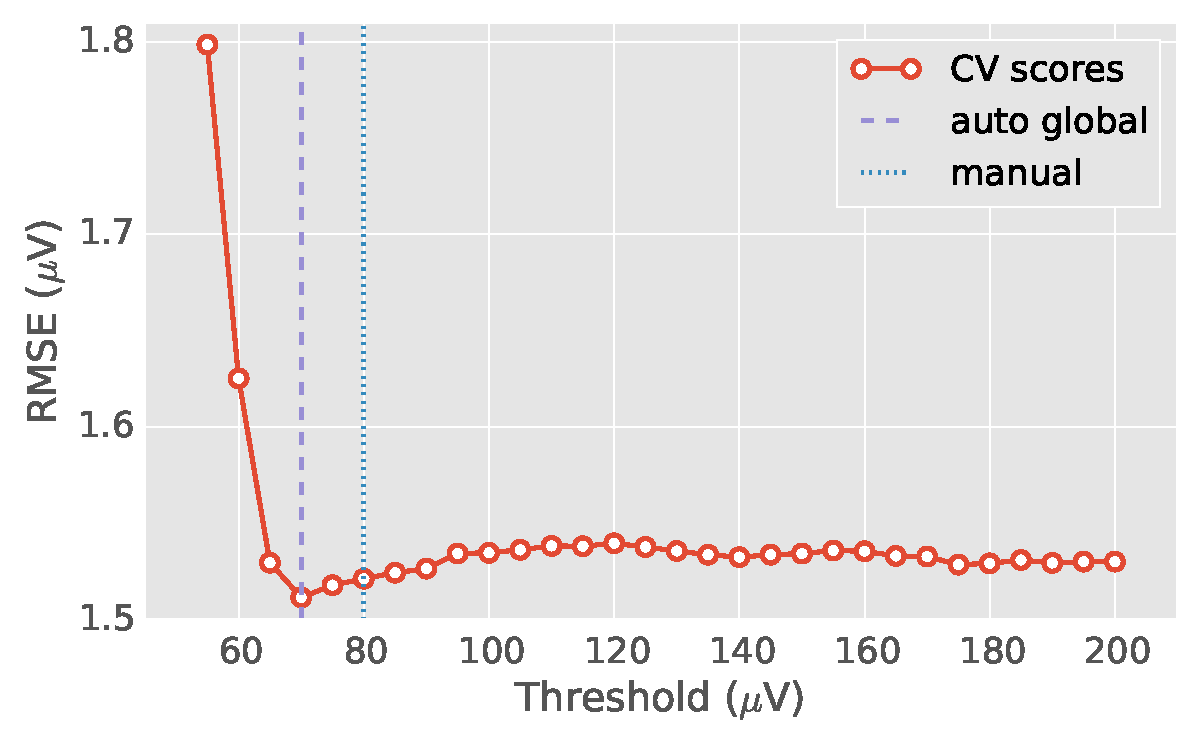
\includegraphics[width=0.65\linewidth]{figures/figure1.pdf}
    \caption[Cross-validation error as a function of peak-to-peak rejection threshold on one EEG dataset.]{Cross-validation error as a function of peak-to-peak rejection threshold on one EEG dataset. The root mean squared error (RMSE) between the mean of the training set (after removing the trials marked as bad) and the median of the validation set was used as the cross-validation metric (Section~\ref{sec:auto_global}). The two insets show the average of the trials as ``butterfly plots" (each curve representing one sensor) for very low and high thresholds. For low thresholds, the RMSE is high because most of the trials are rejected (underfit). At high thresholds, the model does not drop any trials (overfit). The optimal data-driven threshold (\emph{autoreject, global}) with minimum RMSE is somewhere in between. It closely matches the human threshold.}
    \label{fig:cross_val}
\end{figure}

This led us to adopt a pragmatic approach in terms of algorithm design, as it focuses on the tuning of the parameters that M/EEG users presently choose manually. The goal is, not only to obtain high quality data but also to develop a method which is transparent and not too disruptive for the majority of M/EEG users. A first question we address below is: can we improve peak-to-peak based rejection methods by automating the process of trial and error? In the following section, we explain how the widely-known statistical method of cross-validation (see Figure~\ref{fig:cross_val} for a preview) in combination with Bayesian optimization~\citep{snoek2012practical, bergstra2011algorithms} can be employed to tackle the problem at hand. We then explain how this strategy can be extended to set thresholds separately for each sensor and mark trials as bad when a large majority of the sensors have high-amplitude artifacts. This process closely mimics how a human expert would mark a trial as bad during visual inspection. 

In the rest of the paper, we detail the internals of our algorithm, compare it against various state-of-the-art methods, and position it conceptually with respect to these different approaches. For this purpose, we make use of qualitative visualization techniques as well as quantitative reports. In a major validation effort, we take advantage of cleaned up evoked response fields (ERFs) provided by the Human Connectome Project~\citep{larson2013adding} enabling ground truth comparison between alternative methods. This work represents one of the first efforts in reanalysis of the MEG data from the HCP dataset using a toolkit stack significantly different from the one employed by the HCP consortium. The convergence between our method and the HCP MEG pipelines is encouraging and testifies to the success of the community-wide open science efforts aiming at reproducible research. Naturally, we have therefore made our code available online\footnote{\url{https://autoreject.github.io}}. In addition to this, we validated our algorithm on the MNE sample data~\citep{gramfort2013meg}, the multimodal faces dataset~\citep{wakeman2015multi}, and the EEGBCI motor imagery data~\citep{goldberger2000physiobank,schalk2004bci2000}.

A preliminary version of this work was presented in~\citet{jas2016automated}.
\paragraph{Notations} We denote matrices by capital letters $X \in \real^{m \times n}$. The $i$th row of a matrix is indexed by subscripts, as in $X_{i}$, and the entry in the $i$th row and $j$th column is indexed as $X_{ij}$. The matrix $X$ restricted to the rows with indices in the set $\mathcal{G}$ is denoted by $X_\mathcal{G}$. All sets $\mathcal{G}$, $\mathcal{T}$ or $\mathcal{V}$ are written in calligraphic fonts.

\section{Materials and methods}
%
We will first describe how a cross-validation procedure can be used to set peak-to-peak rejection thresholds globally (\textit{i.e.} same threshold for all sensors). This is what we call \textit{autoreject (global)}.

\subsection{Autoreject (global)}
\label{sec:auto_global}
We denote the data matrix by $X \in \real^{N \times P}$ with $N$ trials and $P$ features. These $P$ features are the $Q$ sensor-level time series, each of length $T$ concatenated along the second dimension of the data matrix, such that $P=QT$. We divide the data into $K$ folds (along the first dimension) with training set indices $\mathcal{T}_{k}$ and validation set indices $\mathcal{V}_{k}=[1..N] \setminus {\mathcal{T}_k}$ for each fold $k$ $(1 \leq k \leq K)$. For simplicity of notation, we first define the peak-to-peak amplitude for the $i$th trial and $j$th sensor as the difference between the maximum and the minimum value in that time series:
\begin{equation}
\mathcal{A}_{ij} = \max_{(j-1)T+1 \leq t \leq jT} (X_{it}) - \min_{(j-1)T+1 \leq t \leq jT} (X_{it}) \enspace .
\end{equation}
The set of indices of good trials $\mathcal{G}_k$ in which the peak-to-peak amplitude $\mathcal{A}_{ij}$ for any sensor does not exceed the candidate threshold $\tau$ are generated as
\begin{equation}
\mathcal{G}_k = \{i \in \mathcal{T}_{k} \suchthat \max_{1 \leq j \leq Q} \mathcal{A}_{ij} \leq \tau\}.
\end{equation}
By comparing the peak-to-peak threshold with the maximum of the peak-to-peak amplitudes, we ensure that none of the sensors exceed the given threshold. Once we have applied the threshold on the training set, it is necessary to evaluate how the threshold performs by looking at new data. For this purpose, we consider the validation set. We propose to compare the mean $\overbar{X_{\mathcal{G}_k}}(\tau)$ of good trials in the training set against the median $\widetilde{X_{\mathcal{V}_k}}$ of all trials in the validation set. Using root mean squared error (RMSE) the mismatch $e_{k}(\tau)$ reads as:
\begin{equation}
 e_{k}(\tau) = \fro{\overbar{X_{\mathcal{G}_k}}(\tau) - \widetilde{X_{\mathcal{V}_k}}}.
\label{eq:err} 
\end{equation}
Here, $\fro{\cdot}$ is the Frobenius norm. The rationale for using the median in the validation set is that it is robust to outliers. Indeed, it is far less affected by high-amplitude artifacts than the mean. The threshold with the best data quality (lowest mismatch $e_{k}(\tau)$) on average across the $K$ folds is selected as the optimal threshold. In practice $\tau$ is taken in a bounded interval $[\tau_{\min}, \tau_{\max}]$:
%
\begin{equation}
\tau_{\star} = \underset{\tau \in [\tau_{\min}, \tau_{\max}]} \argmin \frac{1}{K} \sum_{k=1}^{K}  e_{k}(\tau)
\label{eq:best_th}
\end{equation}
Note, that $\widetilde{X_{\mathcal{V}_k}}$ does not depend on $\tau$. Indeed, it would not be wise to restrict the validation set to good trials according to the value of $\tau$. As $\tau$ varies, it would lead to a variable number of validation trials, which would affect the comparison of RMSE across threshold values. The idea of using the median in the context of cross-validation has been previously proposed in the statistics literature in order to deal also with outliers~\citep{zheng1998cross, leung2005cross,de2003robust}.

Figure~\ref{fig:cross_val} (on page~\pageref{fig:cross_val}) shows how the average RMSE changes as the threshold varies for the MNE sample dataset~\citep{gramfort2013meg,mne}. At low thresholds, our model underfits as it drops most of the trials in the data resulting in a noisy average. On the other hand, at high thresholds, the model overfits retaining all the trials in the data including the high-amplitude artifacts. Here the candidate values of $\tau$ were taken on a grid. More details on how to solve \eqref{eq:best_th} will be given in Section~\ref{sec:bayesian_opt}.

\subsection{Autoreject (local)}
\label{sec:auto_local}

\begin{figure}[t]
	\centering
	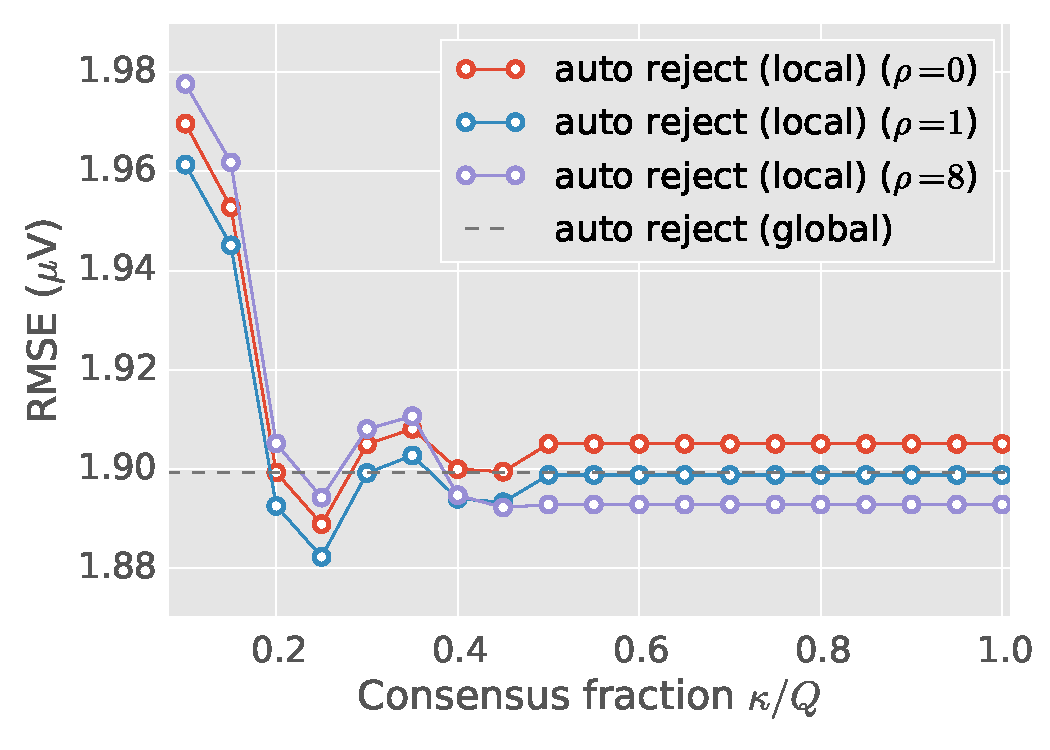
\includegraphics[width=0.65\linewidth]{figures/figure3.pdf}
    \caption[A schematic diagram explaining how \emph{autoreject (local)} works.]{A schematic diagram explaining how \emph{autoreject (local)} works. (A) Each cell here is an element of the transposed indicator matrix $C_{ij}^\top$ described in Section~\ref{sec:auto_local}. Sensor-level thresholds are found and bad segments are marked for each sensor. Bad segments shown in red are where $C_{ij}^\top=1$ (B) Trials are rejected if the number of bad sensors is greater than $\kappa$ and otherwise, the worst $\rho$ sensors (see Equation~\ref{eq:score}) are interpolated.}
    \label{fig:schematic}
\end{figure}

A global threshold common to all sensors, however, suffers from limitations. A common case of failure is when a single sensor is affected (locally or globally) by high-amplitude artifacts. In this case, $\max_{j} \mathcal{A}_{ij}$, which would be the peak-to-peak amplitude that is compared to the threshold, comes from this bad sensor. If the sensor is not repaired or removed, we might end up rejecting a large fraction of otherwise good trials, just because of a single bad sensor. This is certainly not optimal. In fact, a possibly better solution is to replace the corrupted signal in the sensor by the interpolation of the signals in the nearby sensors. A second observation is that sensors can have very different ranges of amplitudes depending on their location on the scalp. A threshold tuned for one sensor may not work as effectively for another sensor. Both of these observations are motivations for estimating rejection thresholds for each sensor separately.

Once we define sensor-wise rejection thresholds $\tau_{\star}^{j}$, we can define an indicator matrix $C_{ij} \in \{0, 1\}^{N \times Q}$ which designates the bad trials at the level of individual sensors. In other words, we have:
\begin{equation}
C_{ij} = \begin{cases} 
0, & \text{if } \mathcal{A}_{ij} \leq \tau^{j}_{\star} \\
1, & \text{if } \mathcal{A}_{ij} > \tau^{j}_{\star}
\end{cases}
\end{equation}
The schematic in Figure~\ref{fig:schematic}A shows a cartoon figure for this indicator matrix $C_{ij}$. Now that we have identified bad sensors for each trial, one might be tempted to interpolate all the bad sensors in each trial. However, it is not as straightforward since in some trials, a majority of the sensors may be bad. These trials cannot be repaired by interpolation and must be rejected. In some other cases, the number of bad sensors may not be large enough to justify rejecting the trial. However, it might already be too much to interpolate all the sensors reliably. In these cases, a natural idea is to pick the worst few sensors and interpolate them. This suggests an algorithm as described in Figure~\ref{fig:schematic}B. Reject a trial only if most sensors ``agree'' that the trial is bad, otherwise interpolate as many sensors as possible. We will denote by $\kappa$ the maximum number of bad sensors in a non-rejected trial and by $\rho$ the maximum number of sensors that can be interpolated. Note that $\rho$ is necessarily less than $\kappa$. The interpolation scheme for EEG uses spherical splines~\citep{perrin1989spherical} while for MEG it uses a Minimum Norm Estimates formulation with spherical harmonics~\citep{hamalainen1994interpreting}. The implementation is provided by MNE-Python~\citep{gramfort2013meg}.

The set of good trials $\mathcal{G}^{\kappa}_k$ in the training set $\mathcal{T}_k$ can therefore be written mathematically as:
%
\begin{equation}
\mathcal{G}^{\kappa}_{k} = \{i \in \mathcal{T}_k \suchthat \sum_{j=1}^{Q} C_{ij} < \kappa \} \enspace .
\end{equation}
%
In the remaining trials, if $\rho < \kappa$, one needs to define what are the worse $\rho$ sensors that shall be interpolated. To do this we propose to rank the sensors for ``badness'' according to a score. A natural strategy to set the score is to use the peak-to-peak amplitude itself:
%
\begin{equation}
s_{ij} = \begin{cases}
\mathcal{A}_{ij} & \text{if } C_{ij} = 1 \\
-\infty & \text{if } C_{ij} = 0
\end{cases}
\label{eq:score}
\end{equation}

The higher the score $s_{ij}$, the worse the sensor. The $-\infty$ score is for ignoring the good sensors in the subsequent step. The following strategy is used for interpolation.
%
%
If the number of bad sensors $\sum_{j'=1}^{Q} C_{ij'}$ is less than $\rho$ we will interpolate all of them. Otherwise, we will interpolate the $\rho$ sensors with the highest scores.
In other words, we interpolate at most $\mathrm{min}(\rho, \sum_{j'=1}^{Q} C_{ij'})$ sensors.
%
%
%
%
%
%
%
%
%
%
%

Denoting by $X^{\rho}_{\mathcal{G}^{\kappa}_k}$ the data in the training set after rejection and cleaning by interpolation, the RMSE averaged over $K$ folds for the parameter pair $(\rho, \kappa)$ therefore becomes:
%
\begin{equation}
\overbar{e}(\rho, \kappa) = \frac{1}{K} \sum_{k=1}^{K} \fro{\overbar{X^{\rho}_{\mathcal{G}^{\kappa}_k}} - \widetilde{X_{\mathcal{V}_k}}}
\end{equation}
where $\fro{\cdot}$ is the Frobenius norm.
Finally, the best parameters $\rho_{*}$ and $\kappa_{*}$ are estimated using grid search~\citep{hsu2003practical}.
%

\subsubsection{Data augmentation}
\label{sec:data_augmentation}

\begin{figure}[ht!]
    \centering
    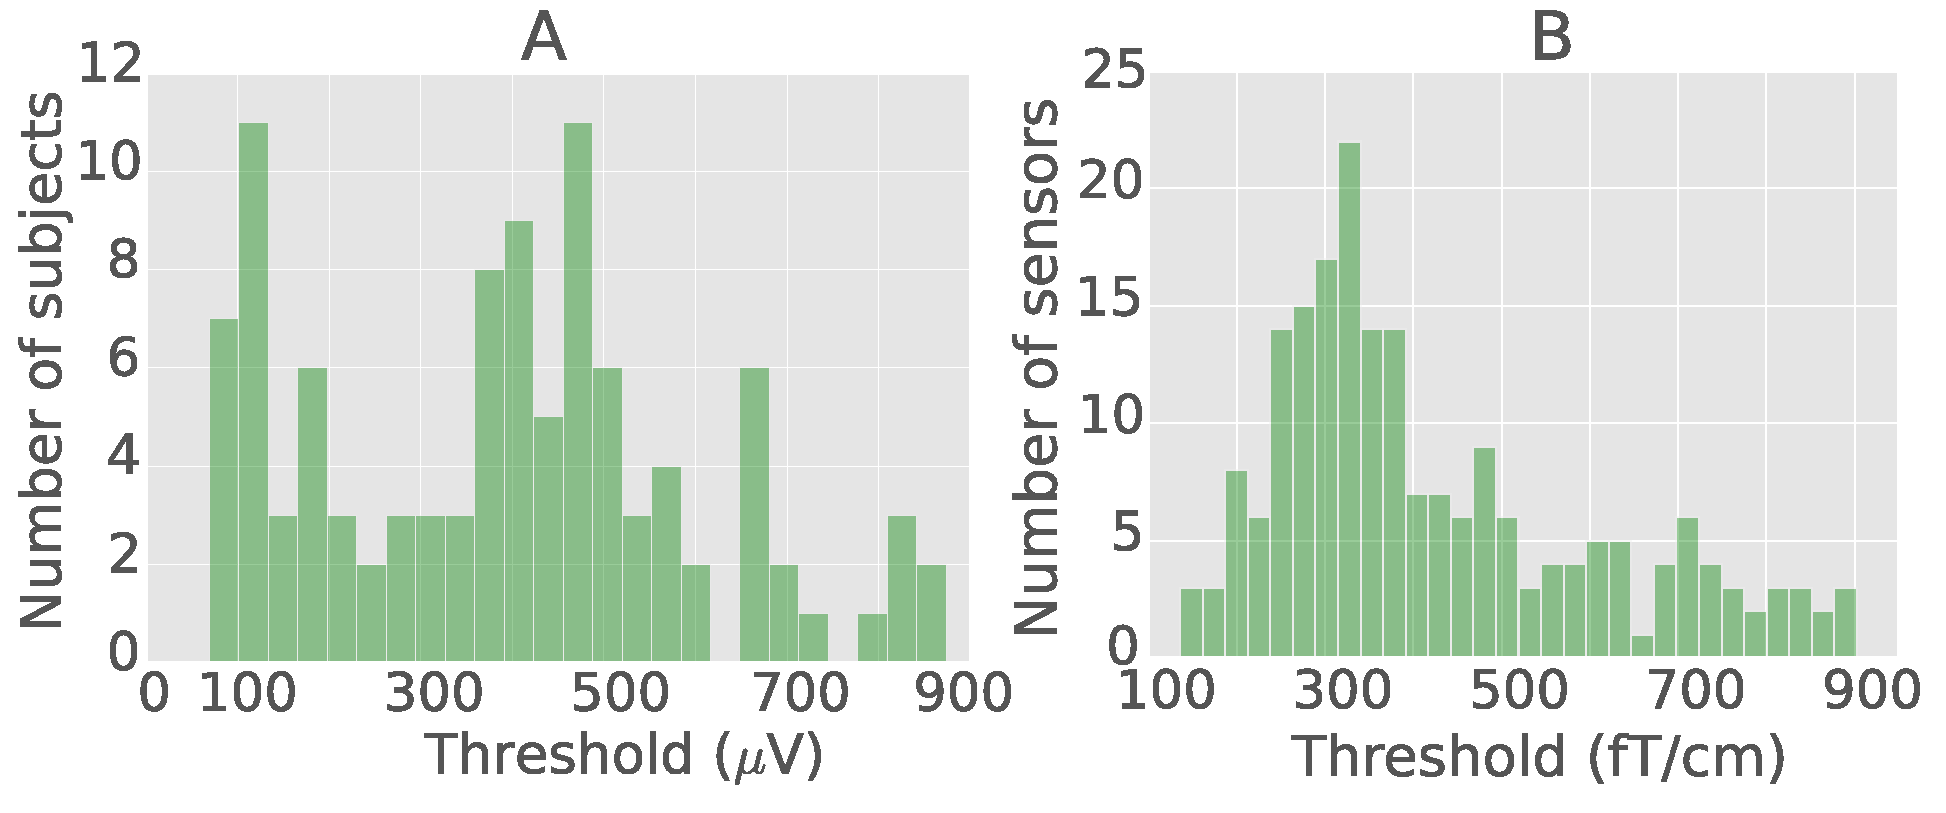
\includegraphics[width=0.8\linewidth]{figures/figure2.pdf}
    \caption[Sequential Bayesian optimization cross-validation curves]{(A) and (B) The cross-validation curve obtained with sequential Bayesian optimization (see Section~\ref{sec:bayesian_opt} for an explanation) for a regular (MEG 2523) and a globally bad sensor (MEG 2443) from the MNE sample dataset. The mean \ac{RMSE} is shown in red circles with the standard deviation in red shades. Vertical dashed line marks the estimated threshold. (C) and (D) Histogram of peak-to-peak amplitudes of trials in the sensor. The histograms are computed separately for the real data (red) and the data interpolated from other sensors (blue). The estimated optimal threshold correctly marks all the trials as bad for the globally bad sensor.}
    \label{fig:cross_val_hist}
\end{figure}

In practice, cross-validation does not work for a globally bad sensor since all the trials are corrupted. In this scenario, the optimal threshold for this bad sensor should be lower than the lowest peak-to-peak amplitude so that all the trials for that sensor are marked as bad. However, even the median of the validation set has been corrupted. The algorithm therefore attempts to keep as many trials as necessary for the average to be close to the corrupted median. Thus, the estimated threshold ends up being higher than what would have been optimal. Recall from Figure~\ref{fig:cross_val} that this is the classic case of an overfitting model. A common strategy in machine learning to reduce overfitting is data augmentation~\citep{krizhevsky2012imagenet}. It basically boils down to using the properties of the data (in our case, this being the physics of the system) to generate additional plausible data.

To implement data augmentation in our model, we interpolate each sensor from all the other $Q-1$ sensors and by doing so, we double the number of trials in the data. In the augmented data, half of the trials contain sensor data. The augmented data matrix is $X^{\textrm{aug}} \in \real^{2N \times P}$. With the augmented data, the median is now closer to the uncorrupted median of the data in that sensor. During cross-validation the folds were stratified so that the number of interpolated trials and original trials in each fold were roughly equal.

\subsection{Search for optimal thresholds using Bayesian optimization}
\label{sec:bayesian_opt}
Now that we have formalized the problem and our approach, we must estimate the threshold $\tau_{\star}$ which minimizes the error defined in Equation~\eqref{eq:err}. A na\"ive strategy is to define a set of equally spaced points over a range of thresholds $[\tau_{\min}, \tau_{\max}]$. The estimated threshold would be the one which obtains the lowest error among these candidate threshold. This is the approach taken in Figure~\ref{fig:cross_val}. The range of thresholds is easy to set as it can be determined from the minimum and maximum peak-to-peak amplitude for the sensor in the augmented data matrix $X^{\textrm{aug}}$. However, it is not obvious how to set the spacing between the candidate thresholds, and experiments showed that varying this spacing could impact the results. If the candidate thresholds are far apart, one might end up missing the optimal threshold. On the other hand, if the thresholds are very dense, it is computationally more demanding.

This motivated us to use Bayesian optimization~\citep{snoek2012practical, bergstra2011algorithms} to estimate the optimal thresholds. It is a sequential approach which decides the next candidate threshold to try based on all the observed thresholds so far. It is based on maximizing an acquisition function given an objective function of samples seen so far (data likelihood) and the prior (typically a \ac{GP}~\citep{rasmussen2006gaussian}). The objective function in our case is the mean cross-validation error as defined in Equations~\eqref{eq:err}. To obtain the next iterate, an acquisition function is maximized over the posterior distribution. Popular choices of the acquisition function include ``probability of improvement'', ``expected improvement'' and ``confidence bounds of the \ac{GP}''~\citep{snoek2012practical}. We pick ``expected improvement'' as it balances exploration (searching unknown regions) and exploitation (maximizing the improvement) strategies without the need of a tuning parameter. For our analysis, we use the scikit-optimize\footnote{https://scikit-optimize.github.io} implementation of Bayesian optimization, which internally uses the Gaussian process module from scikit-learn~\citep{scikit-learn}.

Figure~\ref{fig:cross_val_hist}A and \ref{fig:cross_val_hist}B show the cross-validation curve for a regular sensor and a globally bad sensor in the MNE sample dataset~\citep{mne,gramfort2013meg}. The RMSE is evaluated on thresholds as determined by the Bayesian optimization rather than a uniform grid. These plots also illustrate the arguments presented in Section~\ref{sec:data_augmentation} with respect to data augmentation. The histograms in Figure~\ref{fig:cross_val_hist}C for the interpolated data and the real data are overlapping for the regular sensor. Thus, the estimated threshold for that sensor marks a trial as outlier if its peak-to-peak values is much higher than the rest of the trials. However, in the case of a globally bad sensor, the histogram (Figure~\ref{fig:cross_val_hist}D) is bimodal -- one mode for the interpolated data and one mode for the real data. Now, the estimated threshold is no longer marking outliers in the traditional sense. Instead, all the trials belonging to that sensor must be marked as bad.

\section{Experimental Validation Protocol}

\begin{table}[tb]
{
    \caption{Overview of rejection strategies evaluated\label{tab:strategies}}
       \begin{center}
       \resizebox{\textwidth}{!}{
       \begin{tabular}{l l l l}
        \hline
        \textbf{method} & \textbf{statistical scope} & \textbf{parameter defaults}\\
		% uses sensor positions? / univariate or multivariate
        \hline
        $\text{FASTER}^{a}$ & univariate & threshold on zscore $=$ 3 \\
        $\text{SNS}^{b}$ & multivariate & number of neighbors = 8\\
        $\text{RANSAC}^{c}$ & multivariate outlier detection & \#resamples = 50, fraction of channels = 0.25,\\
        & & threshold on correlation = 0.75, unbroken time = 0.4 \\
        % & minimum correlation, window size, unbroken time & \\
        autoreject & univariate with cross-validation & sensor-level thresholds, $\rho$ and $\kappa$; learned from data \\
        \hline
        \end{tabular}
        }
        \label{table:methods}
        \end{center}
        %\vspace{-0.9em}
        \hspace{1em}
        {\footnotesize
         $^a$\cite{nolan2010faster}, $^b$\cite{de2008sensor},  $^c$\cite{bigdely2015prep}}
}
\end{table}

To experimentally validate \emph{autoreject}, our general strategy is to first visually evaluate the results and thereafter quantify the performance. We describe below the evaluation metric used, the methods we compare against, and finally the datasets analyzed. All general data processing was done using the open source software MNE-Python~\citep{gramfort2013meg}.

\subsection{Evaluation metric}
The evoked response from the data cleaned using our algorithm or a competing benchmark is denoted by $\overbar{X}(method)$. This is compared to the ground truth evoked response $\overbar{X}(clean)$ (See Section~\ref{sec:datasets} to see how these are obtained for different datasets) using:
%
\begin{equation}
\infnorm{\overbar{X}(method) - \overbar{X}(clean)}
\label{eq:infnorm}
\end{equation}
%
where $\infnorm{\cdot}$ is the infinity norm. The reason for using infinity norm is that it is sensitive to the maximum amplitude in the difference signal as opposed to the Frobenius norm which averages the squared difference. The $\infnorm{\cdot}$ is a particularly sensitive metric to quantity artifacts which are also visually striking such as those localized on one sensor or at a given time instant.

\subsection{Competing methods}
\label{sec:competing_methods}

Here, we list the methods that will be quantitatively compared to \emph{autoreject} using the evaluation metric in Equation~\ref{eq:infnorm}. These methods are also summarized for the reader's convenience in Table~\ref{table:methods}.

% \denis{the bullet points were reported to be disturbing by Fede; check that it is consistent with methods}
\begin{itemize}[noitemsep,nolistsep]
\item \emph{No rejection}: It is a simple sanity check to make sure that the data quality upon applying the \emph{autoreject (local)} algorithm does indeed improve. This is the data before the algorithm is applied.
\item \emph{Sensor Noise Suppression (SNS)}: The SNS~\citep{de2008sensor} algorithm, as described in the Introduction (Section~\ref{sec:introduction}), projects the data of each sensor on to the subspace spanned by the principle components of all the other sensors. What it does is regressing out the sensor noise that cannot be explained by other sensors. It works on the principle that brain sources project on to multiple sensors but the noise is uncorrelated across sensors. In practice, not all the sensors are used for projection, but only a certain number of neighboring sensors (determined by the correlation in the data between the sensors).
\item \emph{Fully Automated Statistical Thresholding for EEG artifact Rejection (FASTER)}: It finds the outlier sensor using five different criteria: the variance, correlation, Hurst exponent, kurtosis and line noise. When the z-score of any of these criteria exceeds 3, the sensor is marked as bad according to that criteria. Note that even though FASTER is typically used as an integrated pipeline, here we use the bad sensor detection step, as this is what appears to dominate the bad signals in the case of the HCP data (Section~\ref{sec:datasets}). We take a union of the sensors marked as bad by the different criteria and interpolate the data for those sensors.
\item \emph{Random Sample Consensus (RANSAC)}: We use the RANSAC implemented as part of the PREP pipeline~\citep{bigdely2015prep}. In fact, RANSAC~\citep{fischler1981random} is a well-known approach used to fit statistical models in the presence of outliers in the data. In this approach, adopted for the use case of artifact detection in EEG, a subset of sensors (inliers) are sampled randomly (25\% of the total sensors) and the data in all sensors are interpolated from these inliers sensors. This is repeated multiple times (50 in the PREP implementation) so as to yield a set of 50 time series for each sensor. The correlation between the median, computed instant by instant, of these 50 time series and the real data is computed. If this correlation is less than a threshold (0.75 in the PREP implementation), then the sensor is considered an outlier and therefore marked as bad. It is perhaps worth noting that unlike in the classical RANSAC algorithm, the inlier model is not learned from the data but instead determined from the physical interpolation. A sensor which is bad for more than 40\% of the trials (the unbroken time) is marked as globally bad and interpolated. Even though the method was first proposed on EEG data only, we extended it for MEG data by replacing spline interpolation with field interpolation using spherical harmonics as implemented in MNE~\citep{gramfort2013meg,hamalainen1994interpreting}. Note that this is the same interpolation method that is used by \emph{autoreject (local)}.
\end{itemize}

\subsubsection{Datasets}
\label{sec:datasets}

\begin{table}[!t]
{
    \caption{Overview of datasets analyzed\label{tab:datasets}}
    \resizebox{\textwidth}{!}{
        \begin{tabular}{l l l l l l}
        \hline
         \textbf{Algorithm} & \textbf{Dataset} & \textbf{Acquisition device} & \textbf{Sensors used} & \textbf{\#subjects}\\

\hline
\multirow{2}{*}{autoreject (global)} & MNE sample data & Neuromag VectorView & 60 EEG electrodes & 1\\
& EEGBCI & BCI2000 cap & 64 EEG electrodes & 105\\
\hline
\multirow{3}{*}{autoreject (local)} & MNE sample data & Neuromag VectorView & 60 EEG electrodes & 1\\
& EEG faces & Neuromag VectorView& 60 EEG electrodes & 19\\
& HCP working memory & 4D Magnes 3600 WH& 248 magnetometers & 83\\
        \hline
        \end{tabular}
    }
    \label{table:datasets}
}
\end{table}

We validated our methods on four open datasets with data from over 200 subjects. This allowed us to evaluate experimentally strengths and potential limitations of different rejection methods. The datasets contained either EEG or MEG data. To obtain solid experimental conclusions, diverse experimental paradigms were considered with data from working memory, perceptual and motor tasks.

We detail below how we defined $\overbar{X}(clean)$, the cleaned ground-truth data for two of our datasets -- HCP MEG and EEG faces data. This is perhaps one of the most challenging aspects of this work because the performance is evaluated on real data and not on simulations. An overview of all the datasets used in this study is provided in Table~\ref{table:datasets}.

% One of the most challenging aspects of this work is evaluating the quality of cleaned data. This is due to the difficulty of defining a ground-truth when performance is evaluated on data and not simulations. However, for two of the datasets we described (HCP MEG and EEG faces data), human annotations are available. Such annotations from trained experts obtained independently of the present work offer us an unbiased evaluation setup.

\paragraph{MNE sample data}

The MNE sample data~\citep{gramfort2013meg} is a multimodal open dataset consisting of MEG and EEG data. It has been integrated as the default testing dataset into the development of the MNE software~\citep{gramfort2013meg}. The simultaneous M/EEG data were recorded at the Martinos Center of Massachusetts General Hospital. The MEG data with a Neuromag VectorView system, and an MEG-compatible cap comprising 60 electrodes was used for the EEG recordings. Data were sampled at 150 Hz. In the experiment, auditory stimuli (delivered monoaurally to the left or right ear) and visual stimuli (shown in the left or right visual hemifield) were presented in a random sequence with a stimulus onset asynchrony of 750 ms. The data was low-pass filtered at 40 Hz. The trials were 700 ms long including a 200 ms baseline period which was used for baseline correction.

\paragraph{EEGBCI dataset}

This is a 109-subject dataset (of which we analyzed 105 subjects which can be easily downloaded and analyzed using MNE-Python~\citep{gramfort2013meg}) containing EEG data recording with a 64-sensor BCI2000 EEG cap~\citep{schalk2004bci2000}. Subjects were asked to perform different motor/imagery tasks while their EEG activity was recorded. In the related BCI protocol, each subject performed 14 runs, amounting to a total of 180 trials for hands and feet movements (90 trials each). The data was band-pass filtered between 1 and 40 Hz, and 700 ms long trials were constructed including a 200 ms pre-stimulus baseline period.

\paragraph{EEG faces data (OpenfMRI ds000117)}

The OpenfMRI ds000117 dataset~\citep{wakeman2015multi} contains multimodal task-related neuroimaging data over multiple runs for \ac{EEG}, \ac{MEG} and fMRI. For our analysis, we restrict ourselves to EEG data. The EEG data was recorded using a 70 channel Easycap EEG with electrode layout conforming to the 10-10\% system. Subjects were presented with images of famous faces, unfamiliar faces and scrambled faces as stimuli. For each subject, on average, about 293 trials were available for famous and unfamiliar faces. The authors kindly provided us with run-wise bad sensor annotations which allowed us to conduct benchmarking against human judgement. To generate the ground truth evoked response $\overbar{X}(clean)$, we randomly select 80 percent of the total number of trials in which famous and unfamiliar faces were displayed. In these trials, we interpolated the bad sensors run-wise. Then, we removed physiological artifacts (heart beat and eye blinks) using Independent Component Analysis (ICA)~\citep{vigario2000independent}. Following the ICA pipelines recommended by the MNE-Python software, the bad ICA components were marked automatically using cross-trial phase statistics~\citep{dammers2008integration} for ECG (threshold=0.8) and adaptive z-scoring (threshold=3) for EOG components. The evoked response from the cleaned data $\overbar{X}(method)$ is computed from the remaining 20 percent trials cleaned using either \emph{autoreject (local)} or \emph{RANSAC} (see Section~\ref{sec:benchmark_sensors} for a description of this method). Computing the ground-truth evoked potential from a large proportion of trials minimized the effect of outliers in the average. However, it is noteworthy that this choice of assigning fewer trials to the estimation with rejection algorithms acts in a conservative sense: each unnoticed bad trial may affect the ensuing evoked potentials more severely.

\paragraph{Human Connectome Project (HCP) MEG data}

The HCP dataset is a multimodal reference dataset realized by the efforts of multiple international laboratories around the world. It currently provides access to both task-free and task-related data for more than 900 human subjects with functional MRI data, 95 of which have presently also MEG~\citep{larson2013adding}. An interesting aspect of the initiative is that the data provided is not only in unprocessed BTi format, but also processed using diverse processing pipelines. These include annotations of bad sensors and corrupted time segments for the \ac{MEG} data derived from automated pipelines and supplemented by human inspection. The automated pipelines are based on correlation between neighboring sensors, z-score metrics, ratio of variance to neighbors, and \ac{ICA} decomposition. Most significant for our purposes, the clean average response $\overbar{X}(clean)$ is directly available. It allows us to objectively evaluate the proposed algorithm against state-of-the-art methods by reprocessing the raw data and comparing the outcome with the official pipeline output.

The HCP MEG dataset provides access to MEG recordings from diverse tasks, \textit{i.e.}, a motor paradigm, passive listening and working memory. Here, we focused on the working memory task for which data is available for 83 subjects out of 95. A considerable proportion of subjects were genetically related, but we can ignore this information as the purpose of our algorithm is artifact removal rather than analyzing brain responses. For each subject two runs are available. Two classes of stimuli were employed, faces and tools. Here, we focused on the MEG data in response to stimulus onsets for the ``faces" condition.

The MEG data were recorded with a wholehead MAGNES 3600 (4D Neuroimaging, San Diego, CA) in a magnetically shielded room at Saint Louis University. The system comprises 248 magnetometers and 23 reference sensors to capture environmental signals. Time windows precisely matched values used by the HCP ``eravg'' pipeline with onsets and offsets at $-1.5$\,s and $2.5$\,s before and after the stimulus event, respectively. As in the HCP pipeline, signals were down-sampled to $508.63$\,Hz and band-pass filtered between 0.5--60\,Hz. As it is commonly done with BTi systems, reference sensors at the periphery of the head were used to subtract away environmental noise. Given the linearity of Maxwell equations in the quasi-static regime, a linear regression model was employed. More precisely, signals from reference sensors are used as regressors in order to predict the MEG data of interest. The ensuing signal explained by the reference sensors in this model was then removed. The HCP preprocessing pipeline contains two additional steps: ICA was used to remove components not related to brain activity (including eye blinks and heart beats) and then bad trials and bad segments were removed with a combination of automated methods as well as annotations by a human observer. To have a fair comparison and focus on the latter step, the ICA matrices provided by the HCP consortium were applied to the data. We interpolated the missing sensors in $\overbar{X}(clean)$ so that it has the same dimensions as the data from $\overbar{X}(method)$. All the algorithms were executed separately on each run and the evoked response of the two runs was averaged to get $\overbar{X}(method)$.

To enable easy access of the files along with compatibility in MNE-Python, we make use of the open source MNE-HCP package\footnote{http://mne-tools.github.io/mne-hcp/}. For further details on the HCP pipelines, the interested reader can consult the related paper by \citet{larson2013adding} and the HCP S900 reference manual for the MEG3 release.

% automated, non-automated is actually a continuum

\section{Results}
\label{sec:results}

We conducted qualitative and quantitative performance evaluations of \emph{autoreject} using four different datasets comparing it to a baseline condition without rejection as well as three different alternative artifact rejection procedures.

\subsection{Peak-to-peak thresholds}

\begin{figure}[htb!]
	\centering
	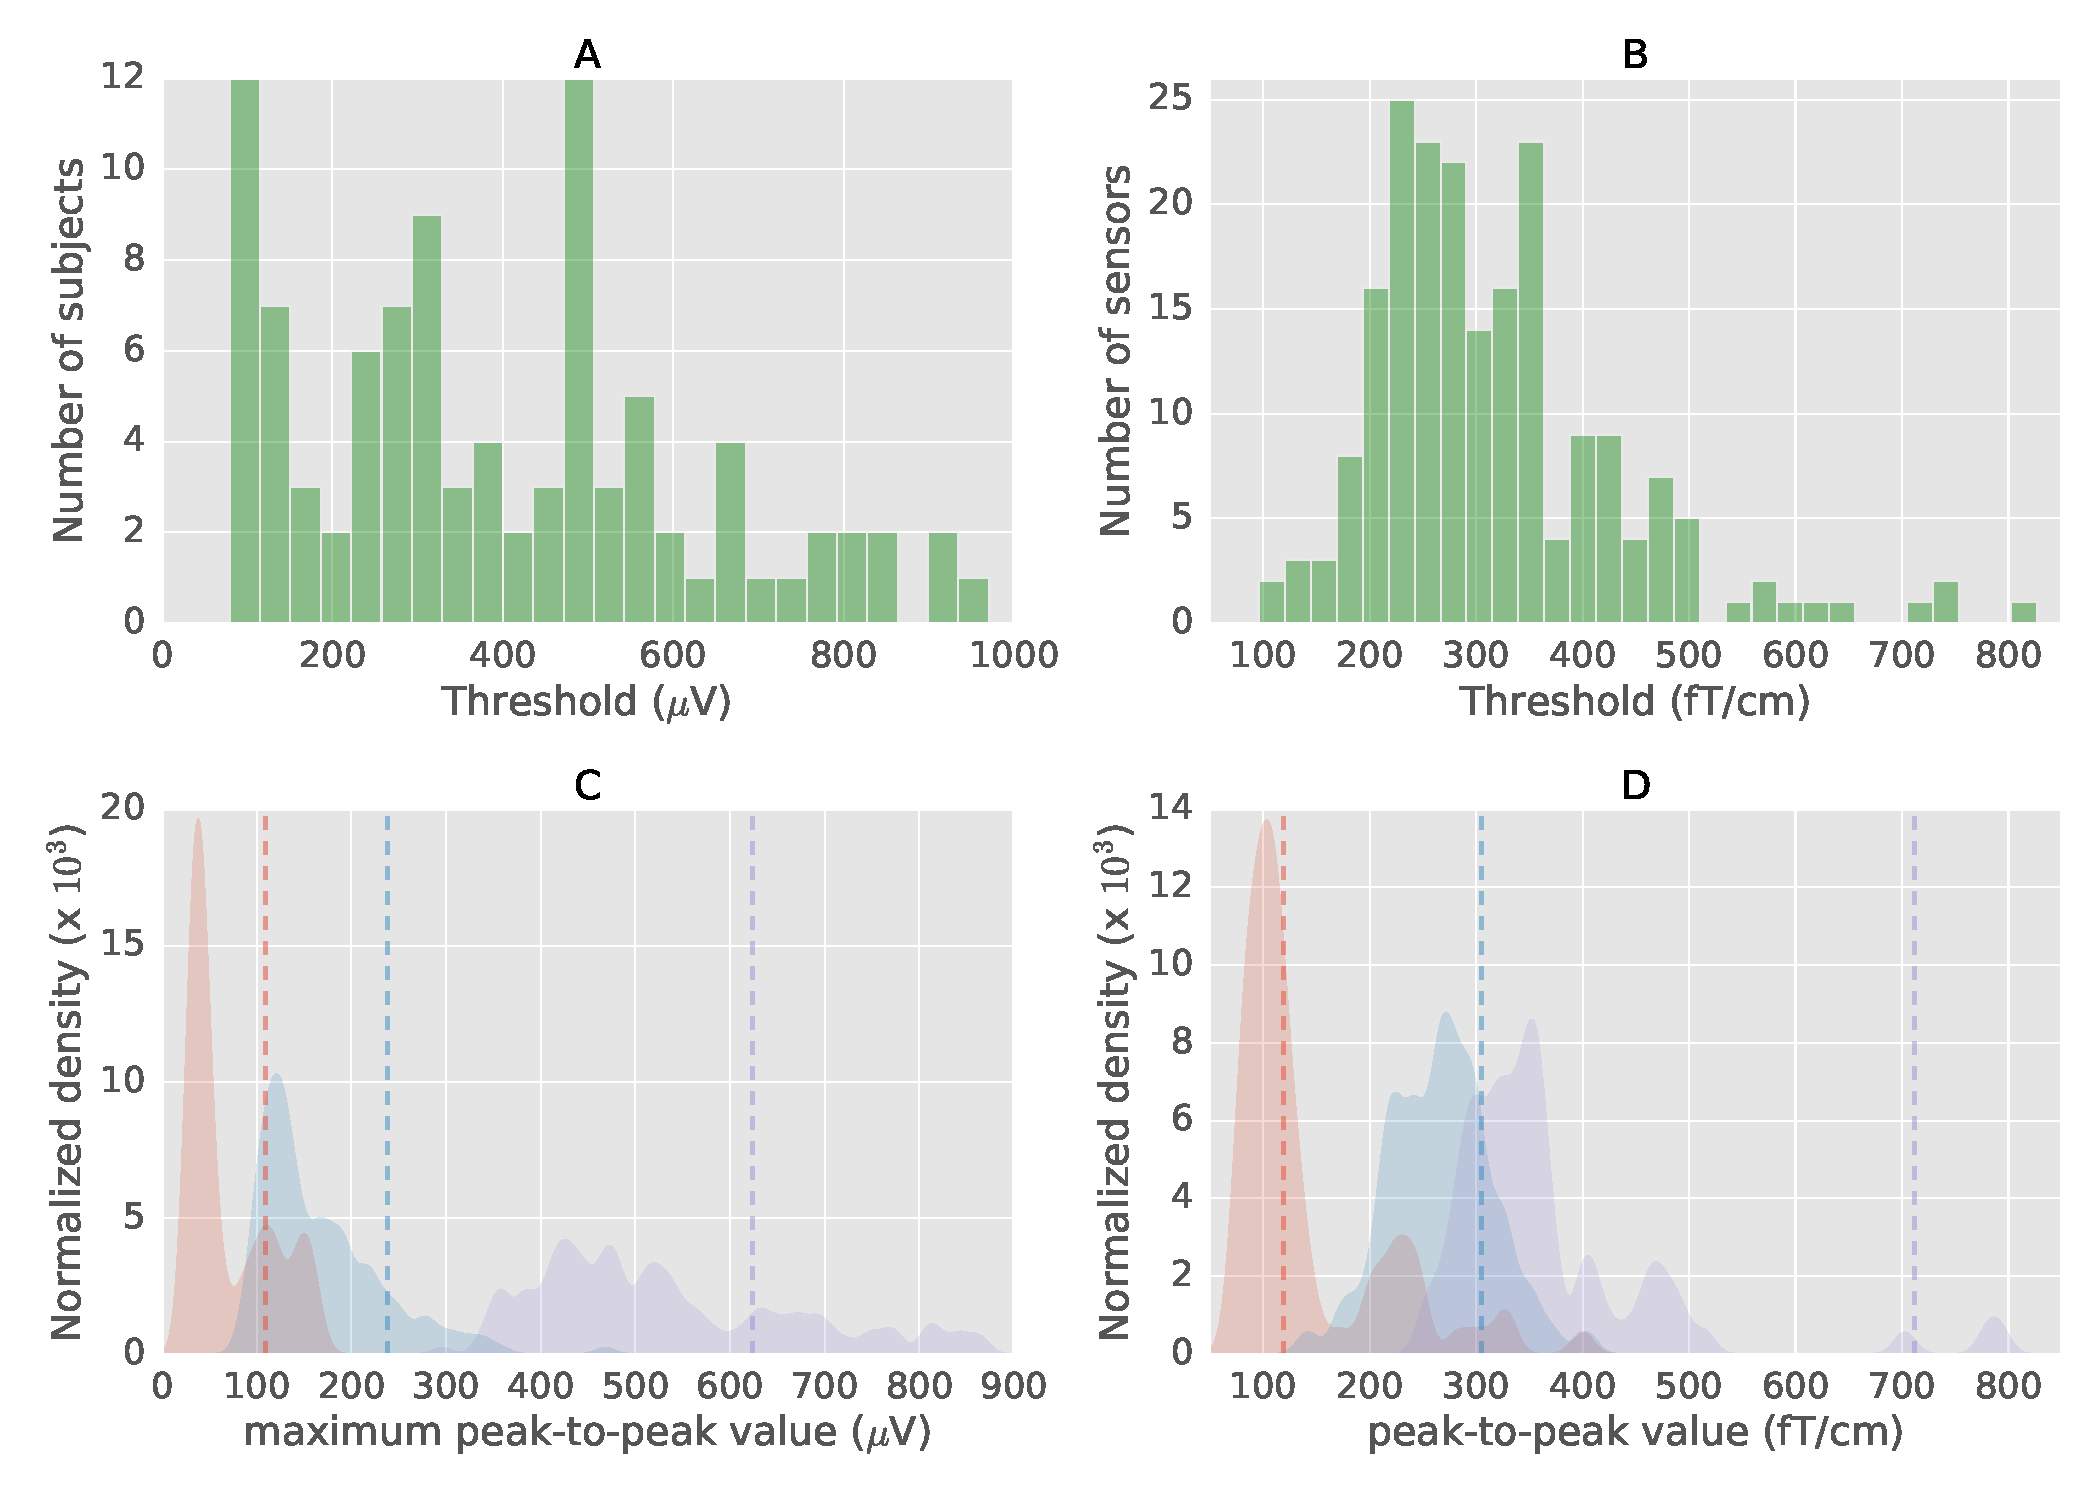
\includegraphics[width=0.9\linewidth]{figures/figure6.pdf}
    \caption[Histograms and kernel density plots of peak-to-peak thresholds.]{A. Histogram of thresholds for subjects in the EEGBCI dataset with \emph{autoreject (global)} B. Histogram of sensor-specific thresholds in gradiometers for the MNE sample dataset (Section~\ref{sec:results}). C. Normalized kernel density plots of maximum peak-to-peak value across sensors for three subjects in the EEGBCI data. Vertical dashed lines indicate estimated thresholds. Density plots and thresholds corresponding to the same subject are the same color. D. Normalized Kernel Density plots of peak-to-peak values for three MEG sensors in the MNE sample dataset. The threshold indeed has to be different depending on the data (subject and sensor).}
    \label{fig:hist}
\end{figure}

First, let us convince ourselves that the peak-to-peak thresholds indeed need to be learned. In Figure~\ref{fig:hist}A, we show a histogram of the thresholds learned on subjects in the EEGBCI dataset using \emph{autoreject (global)}. This figure shows that thresholds vary a lot across subjects. One could argue that this is due to variance in the estimation process. To rule out such a possibility, we plotted the distribution of maximum peak-to-peak thresholds as kernel density plots in Figure~\ref{fig:hist}C for three different subjects. We can see that these distributions are indeed subject dependent, which is why a different threshold must be learned for each subject. In fact, if we were to use a constant threshold of $150 \mu{V}$, in $17\%$ of the subjects, all the trials would be dropped in one of the two conditions. Of course, from Figure~\ref{fig:hist}A, we can now observe that $150 \mu{V}$ is not really a good threshold to choose for many subjects.
%

We show here the maximum peak-to-peak amplitude per sensor because this is what decides if a trials should be dropped or not in the case of \emph{autoreject (global)}. Note that, if instead, we examined the distribution of peak-to-peak amplitudes across all sensors and trials, we would see a quasi-normal distribution. When all the sensors are taken together, a ``smoothing" effect is observed in the distribution. This is a consequence of the central limit theorem. This also explains why we cannot learn a global threshold using all the peak-to-peak amplitudes across trials and sensors.

With the \emph{autoreject (local)} approach, a threshold is estimated for each sensor separately. The histogram of thresholds for the MNE sample dataset is plotted in Figure~\ref{fig:hist}B. It shows that the threshold varies even across homogeneous MEG sensors. Figure~\ref{fig:hist}D shows the distribution of peak-to-peak thresholds for three different MEG sensors. This graph confirms actual sensor-level differences in amplitude distributions, which was also previously reported in the literature~\citep{junghofer2000statistical}. With this work, we go one step further by learning automatically the thresholds in a data-driven way rather than asking users to mark them interactively.

\begin{figure}[htb!]
	\centering
	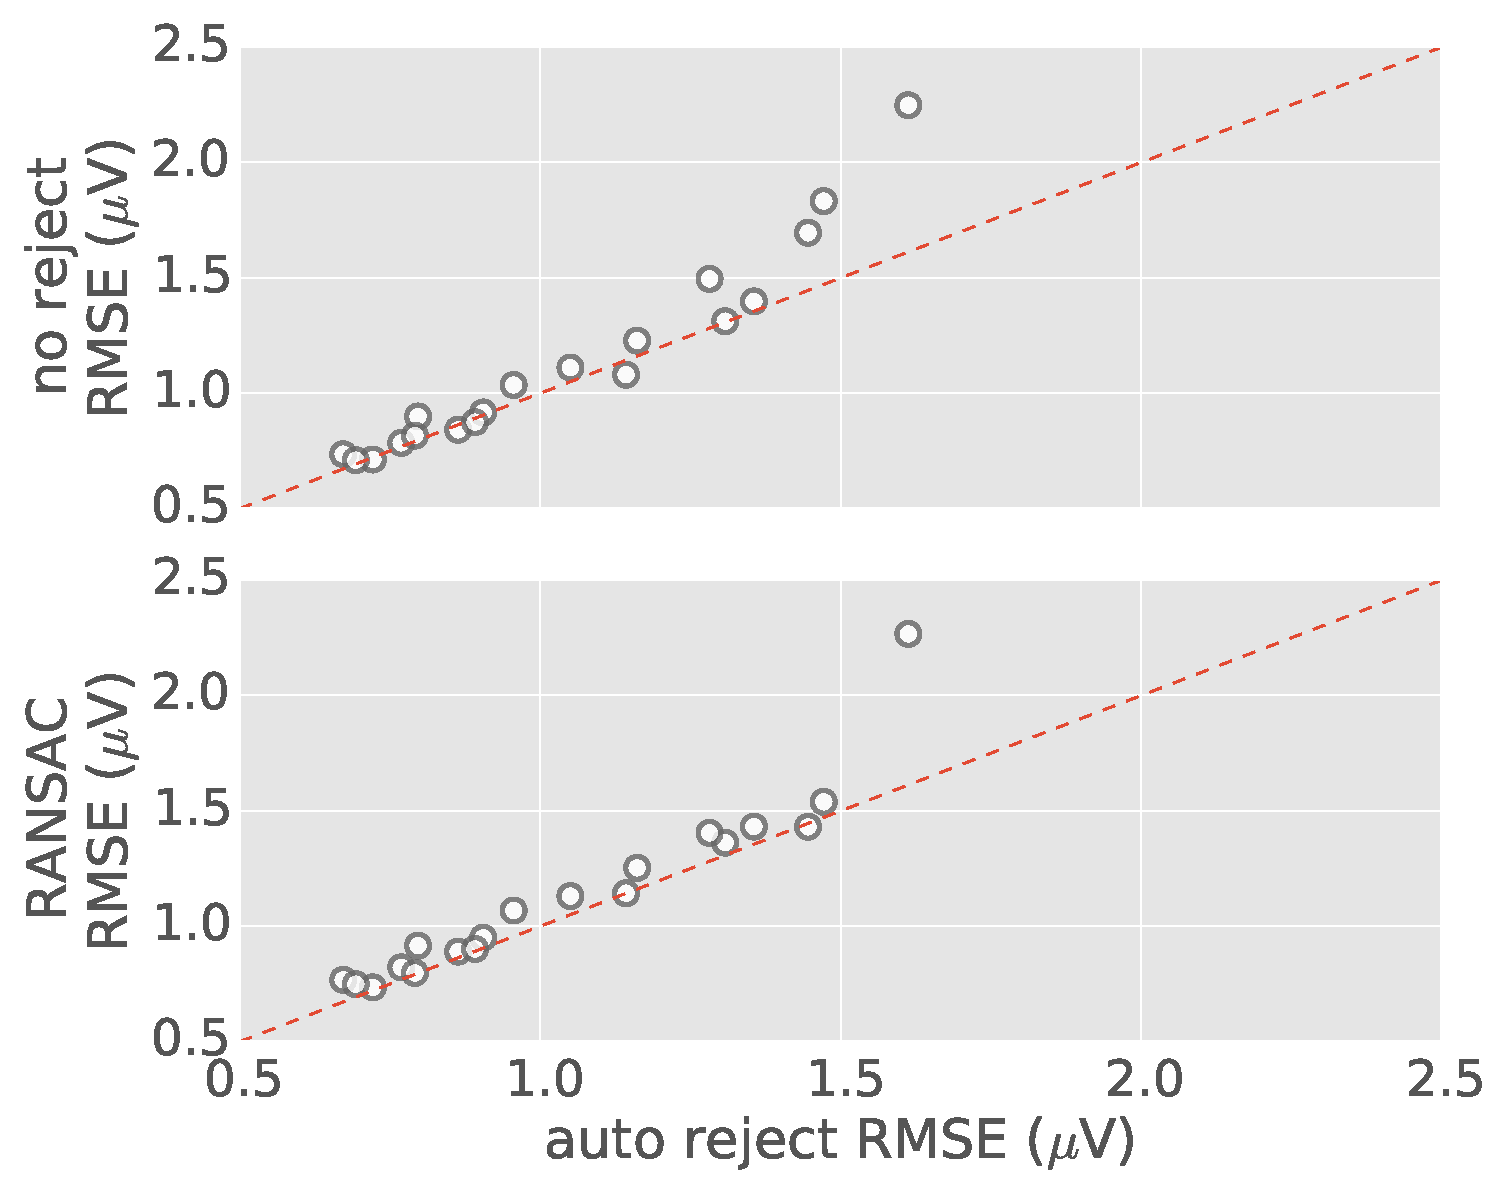
\includegraphics[width=0.9\linewidth]{figures/figure5.pdf}
    \caption[The evoked response (average of data across trials) on three different datasets before and after applying \emph{autoreject}]{The evoked response (average of data across trials) on three different datasets before and after applying \emph{autoreject} --- the MNE sample data, the HCP data and the EEG faces data. Each sensor is a line on the plots. On the left, manually annotated bad sensors are shown in red. The algorithm finds the bad sensors automatically and repairs them for the relevant trials. Note that it can even fix multiple sensors at a time and works for different modalities of data acquisition.}
    \label{fig:sample_evoked}
\end{figure}

\subsection{Visual quality check}

\begin{figure}[htb!]
    \centering
    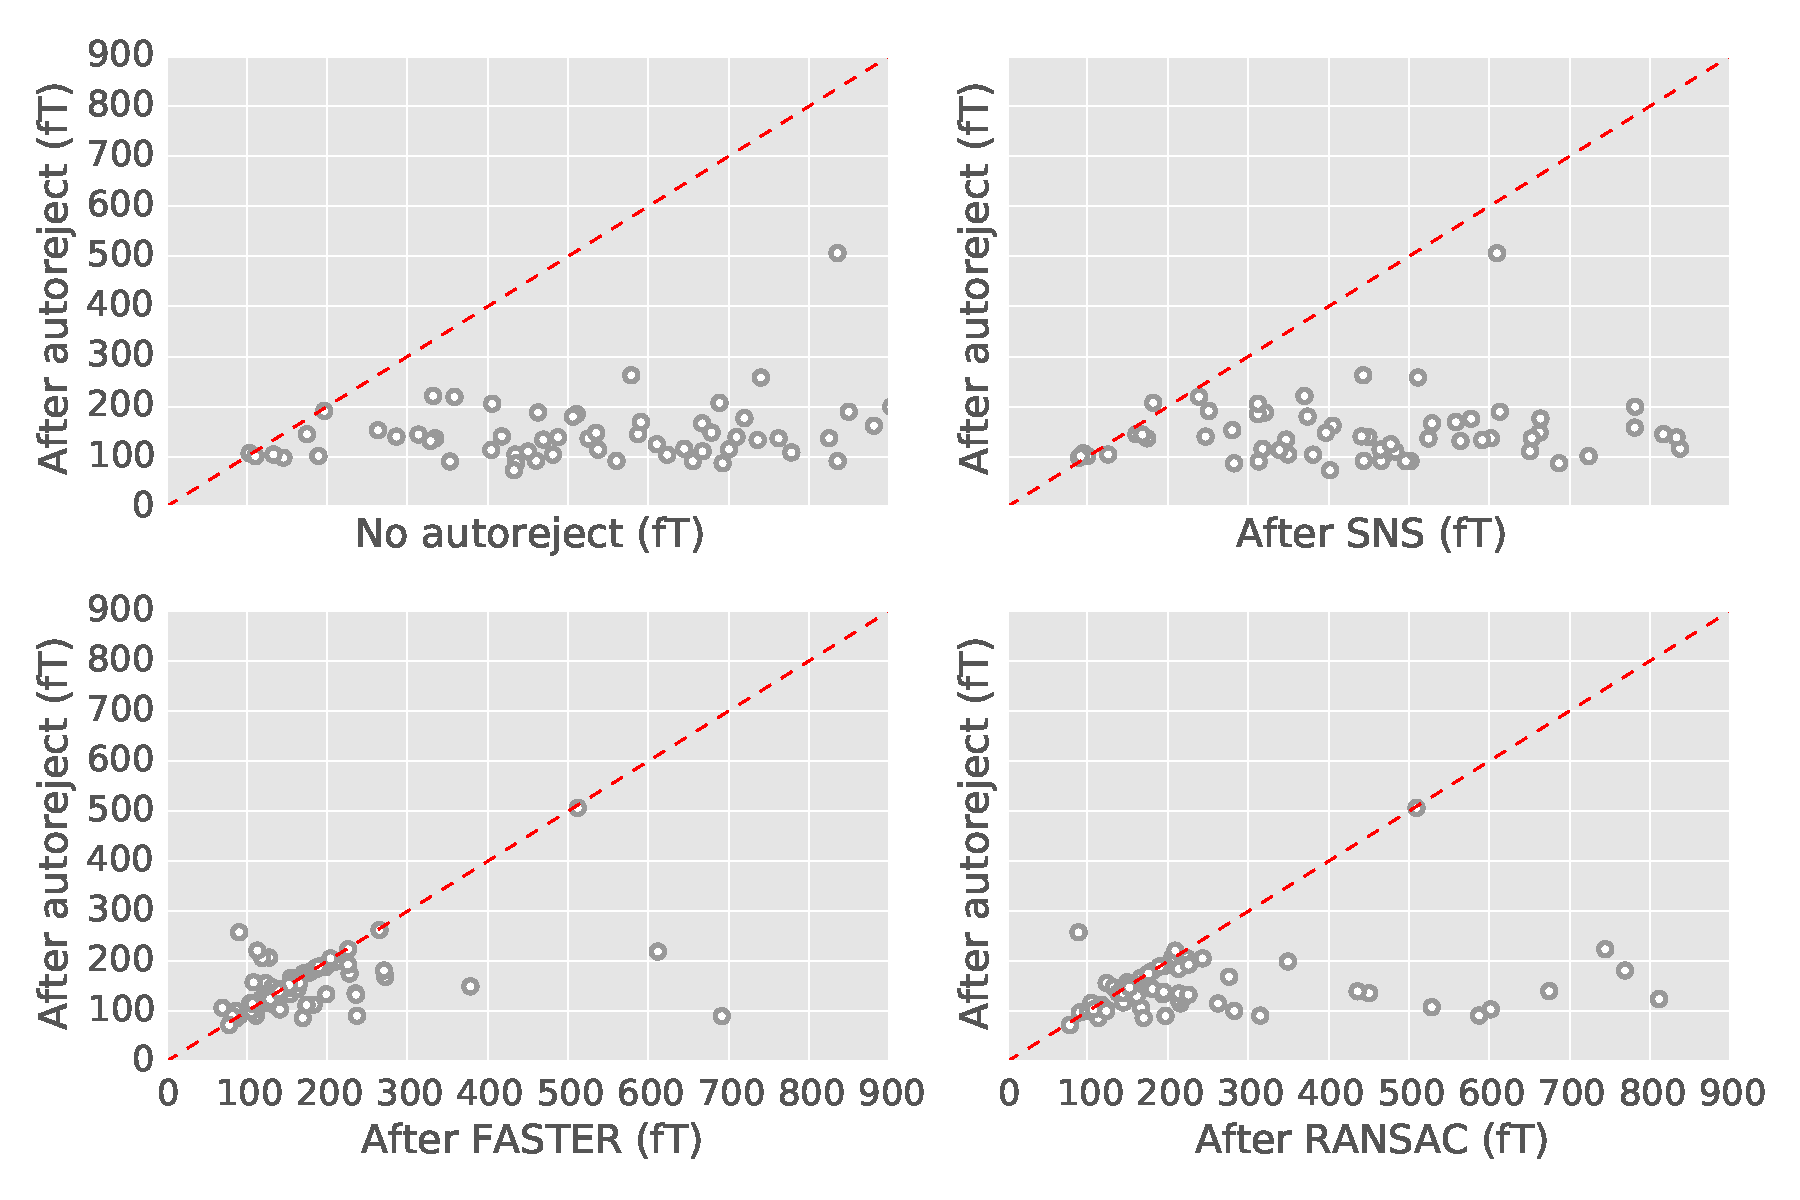
\includegraphics[width=0.8\linewidth]{figures/figure4.pdf}
    \caption[Scatter plots for the results with the HCP data.]{Scatter plots for the results with the HCP data. For each method, the $\infnorm{\cdot}$ norm of the difference between the HCP ground truth and the method is taken. Each circle is a subject. (A) \textit{autoreject (local)} against no rejection, (B) \textit{autoreject (local)} against Sensor Noise Suppression (SNS) (SNS), (C) \textit{autoreject} against FASTER, (D) \textit{autoreject (local)} against RANSAC. Data points below the dotted red line indicate subjects for which \textit{autoreject (local)} outperforms the alternative method.}
    \label{fig:hcp_scatter}
\end{figure}

\begin{figure}[htb!]
    \centering
    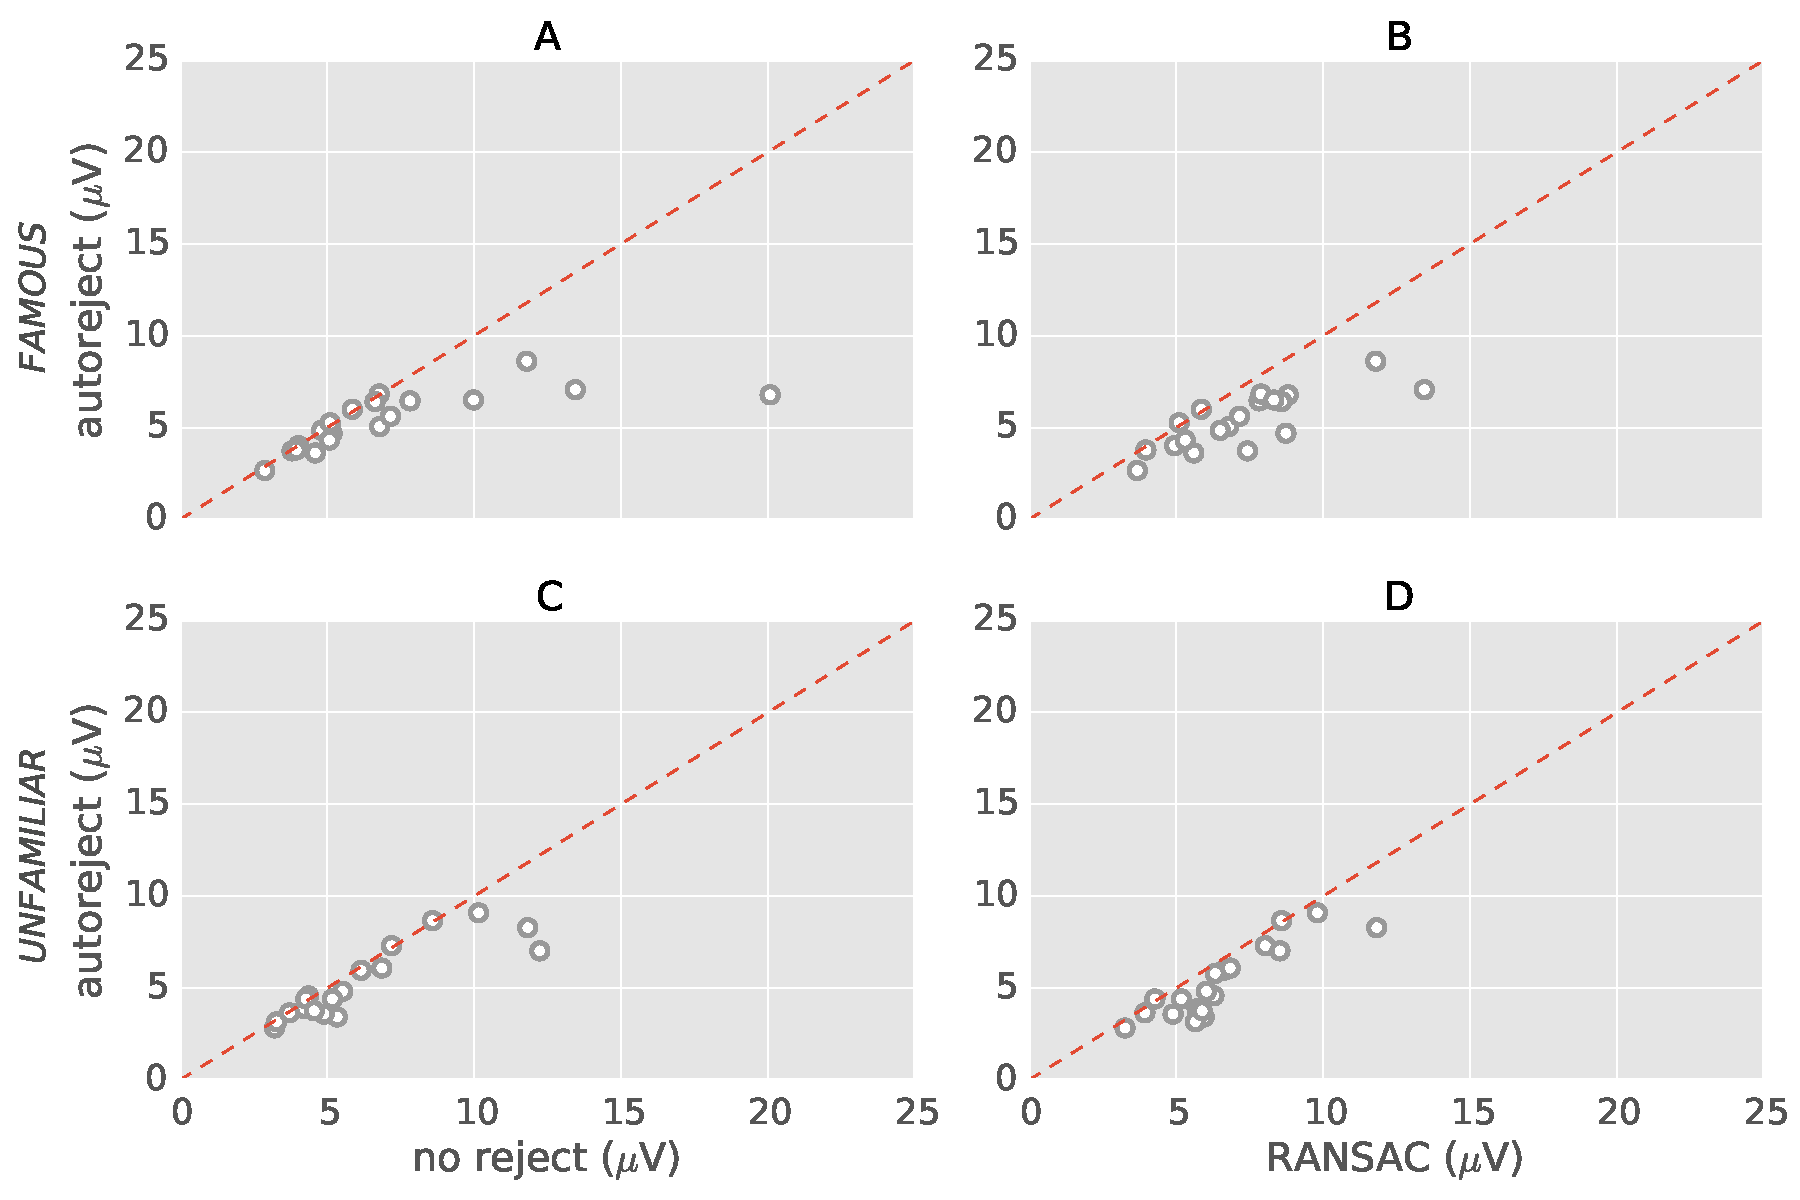
\includegraphics[width=0.8\linewidth]{figures/figure7.pdf}
    \caption[Scatter plots for the results with the 19 subjects from Faces dataset.]{Scatter plots for the results with the 19 subjects from Faces dataset. The first row (A) and (B) is for the condition ``famous" and the second row (C) and (D) is for the condition ``unfamiliar" faces. For each method, the $\infnorm{\cdot}$ norm of the difference between the ground truth and the estimates is computed. Each circle is a subject. Data points below the dotted red line indicate subjects for which \textit{autoreject (local)} outperforms the alternative method.}
    \label{fig:dgw_scatter}
\end{figure}

The average response plotted in a single graph, better known as ``butterfly plots'', constitutes a natural way to visually assess the performance of the algorithm for three different datasets -- MNE sample data, HCP MEG data, and EEG faces data. In Figure~\ref{fig:sample_evoked}, the subplots in the left column show the evoked response with the bad sensors marked in red. Right subplots, show data after applying the \emph{autoreject (local)} algorithm, with the repaired bad sensors in red. The algorithm works for different acquisition modalities -- MEG and EEG, and even when multiple sensors are bad. A careful look at the results, show that \emph{autoreject (local)} does not completely remove eyeblinks in the data as some of the blinks are time-locked to the evoked response. We will later discuss (Section~\ref{sec:discussion}) the possible solutions of applying ICA-based artifact correction in combination with \emph{autoreject (local)}.

\subsection{Quantification of performance and comparison with state-of-the-art}
\label{sec:benchmark_sensors}

We now compare these algorithms to \emph{autoreject (local)} using the data quality metric defined in Equation~\eqref{eq:infnorm} (See Appendix~\ref{chapter:appendix} for explanation as to why $l_\infty$ norm is better than $l_2$ norm). 
We are interested not only in how the algorithms perform on average but at the level of individual subjects. To detail single subject performance, we present the data quality as scatter plots where each axis corresponds to the performance of a method. Figure~\ref{fig:hcp_scatter}, contains results on the HCP MEG data. We can observe from the top-left subplot of the figure that \emph{autoreject (local)} does indeed improve the data quality in comparison to the \emph{no rejection} approach. In Figure~\ref{fig:hcp_scatter}B, \emph{autoreject (local)} is compared against SNS. The SNS algorithm focuses on removing noise isolated on single sensors. Its results can be affected by the presence of multiple bad sensors and globally bad trials. This explains why \emph{autoreject (local)} outperforms SNS is this setting. In Figure~\ref{fig:hcp_scatter}C, we compare against FASTER. Even though \emph{autoreject (local)} is slightly worse than FASTER for a few subjects, FASTER is clearly much worse than \emph{autoreject (local)} for at least 3 subjects, and \emph{autoreject (local)} yields therefore less errors on average. Finally, Figure~\ref{fig:hcp_scatter}D shows comparison to RANSAC. In the PREP implementation, this algorithm is not fully data-driven in the classic sense of RANSAC. This is due to the fact that the inlier model is not learned but rather derived from the physics of the interpolation. It is therefore an algorithm which is conceptually close to \emph{autoreject}. However, a critical difference is that the parameters of this method still need to be tuned. This can be a problem as these parameters can be suboptimal on some datasets. Some experiments showed that it is for example the case for the EEG faces data, where it is possible to obtain better results by manually tuning the RANSAC parameters, rather than using the values proposed by the original authors.

Figure~\ref{fig:dgw_scatter} presents scatter plots for the EEG faces data.
%
Here, we restrict our comparison to RANSAC as it is conceptually the closest to \emph{autoreject}. On this data, we apply the algorithms on both the conditions -- famous and unfamiliar faces. It should be noted that the ground truth for this data was generated automatically with no additional annotations from human experts. However, a sanity check was performed on the ground truth by visual inspection. Here too, \emph{autoreject} offers good results across all subjects, and even for the subjects for which RANSAC underperforms.

\clearpage
\begin{sidewaysfigure}
	\centering
	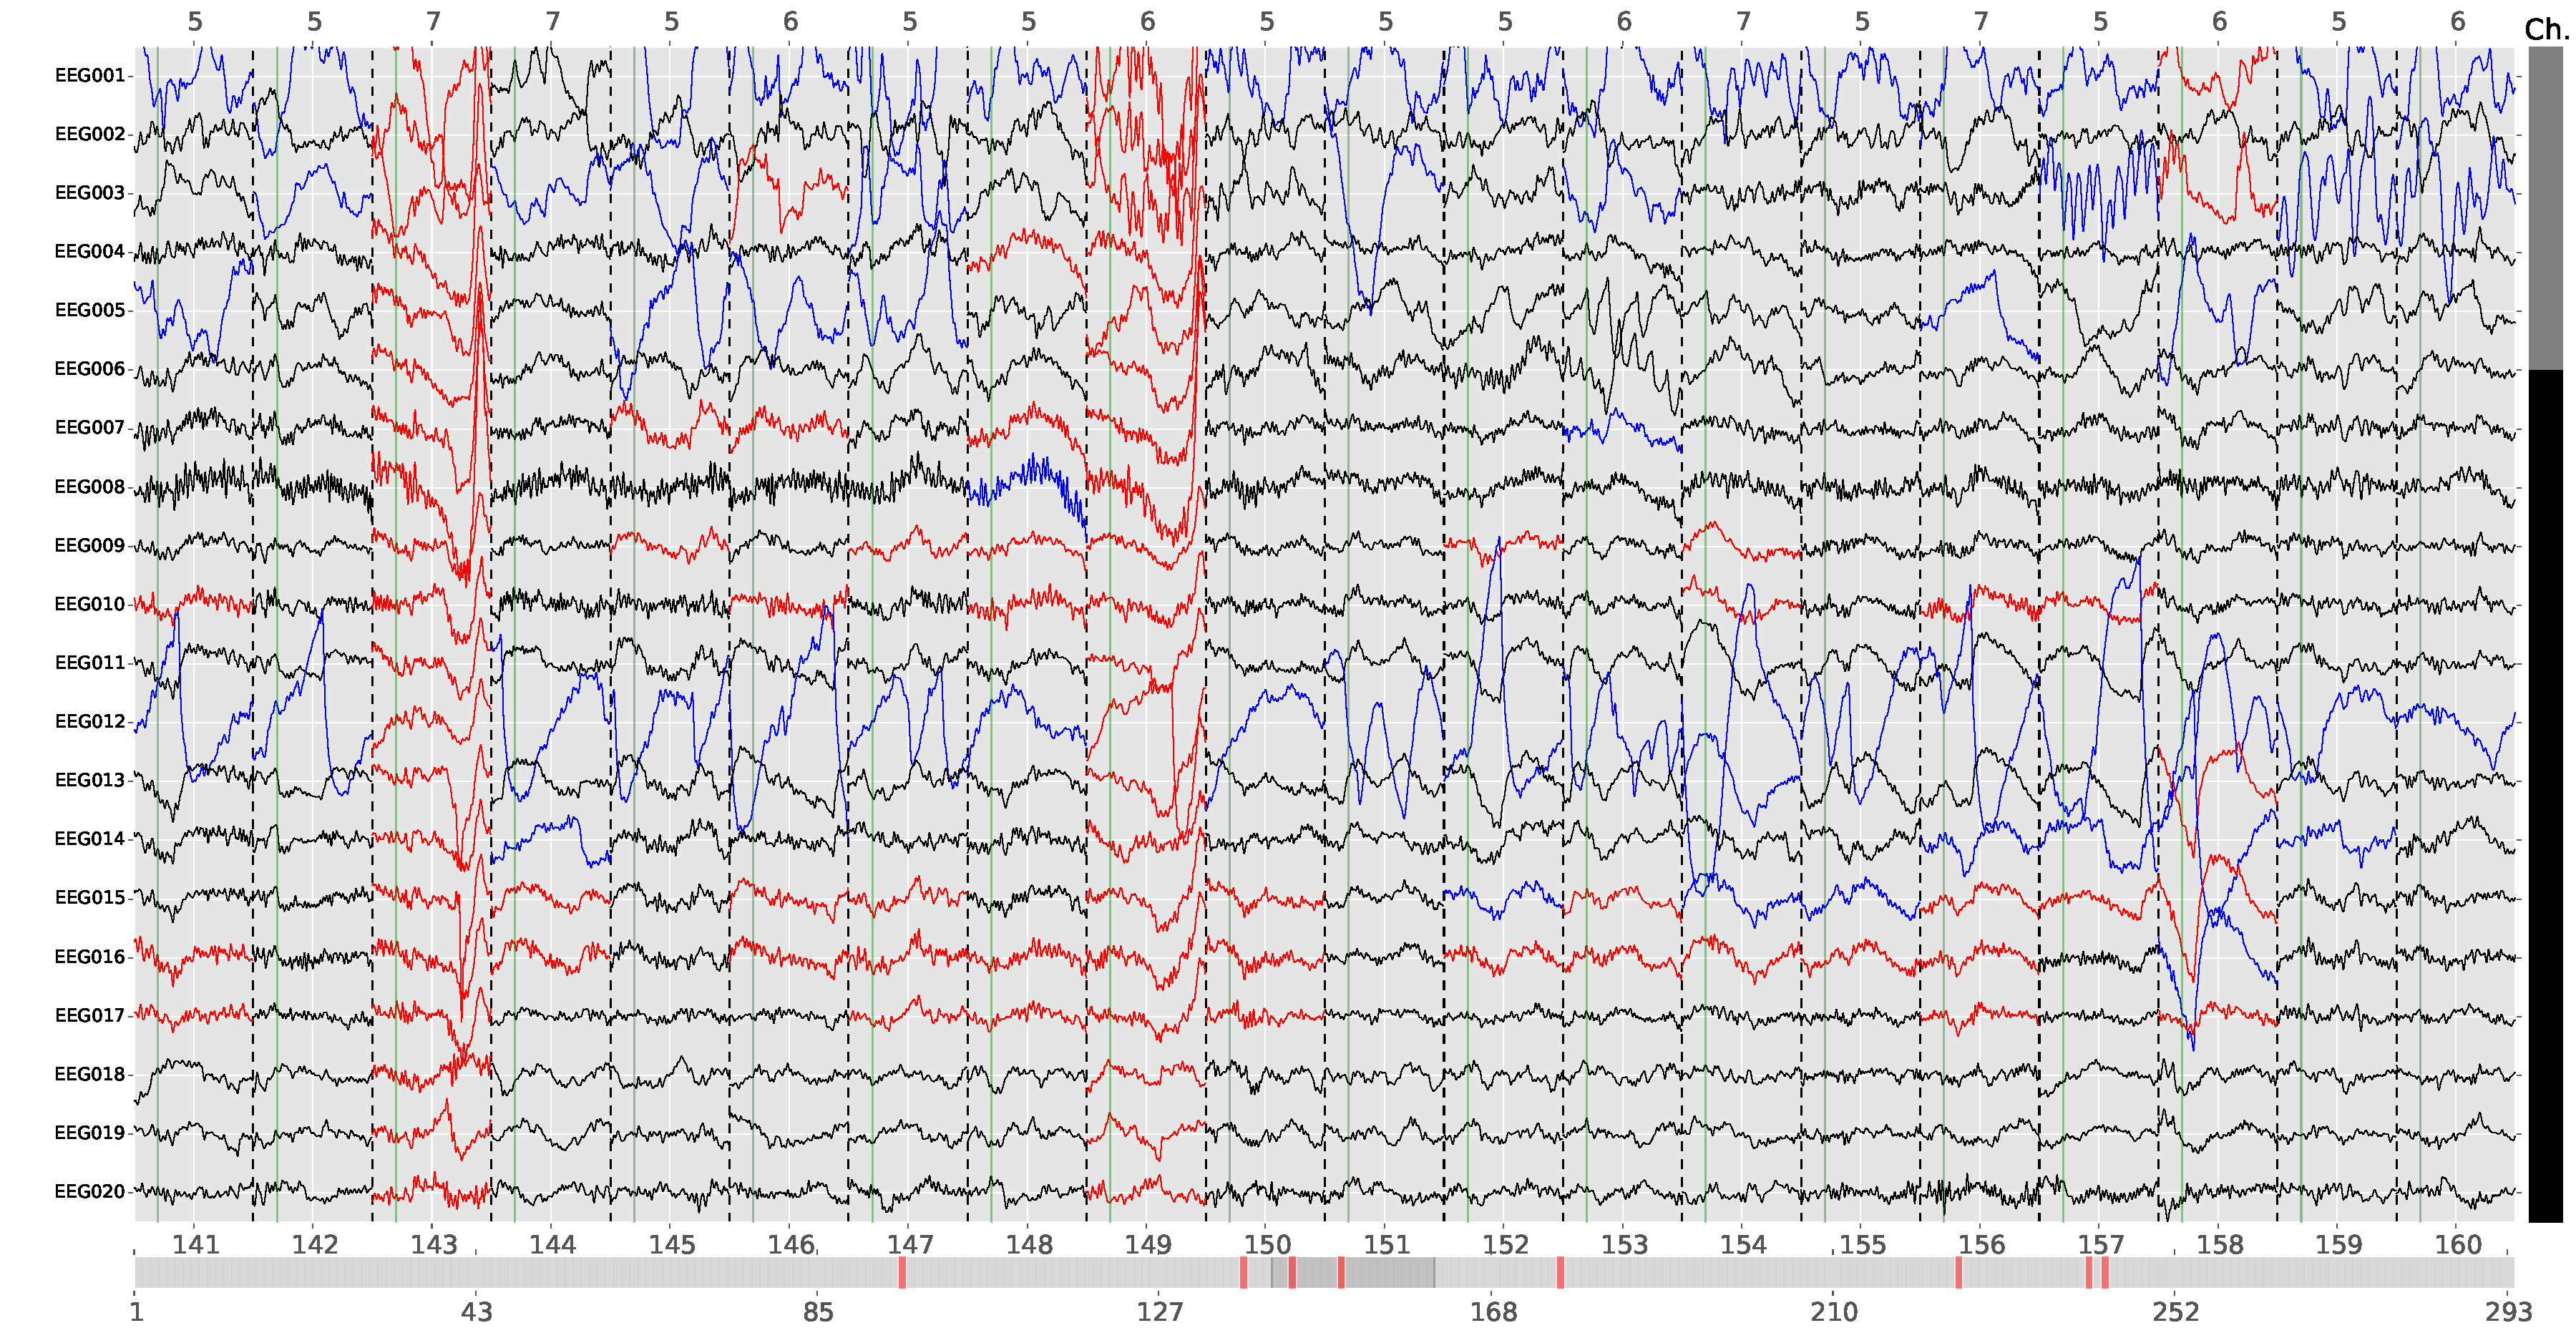
\includegraphics[width=\textwidth]{figures/figure8.pdf}
    \caption[An example diagnostic plot from an interactive viewer with \emph{autoreject (local)}]{An example diagnostic plot from an interactive viewer with \emph{autoreject (local)}. The data plotted here is subject 16 for the condition `famous' in the EEG faces data. Each row is a different sensor. The trials are concatenated along the x axis with dotted vertical lines separating consecutive trials. Each trial is numbered at the bottom and its corresponding trigger code is at the top. The horizontal scroll bar at the bottom allows browsing trials and the vertical scroll bar on the right is for browsing sensors. A trial which is marked as bad is shown in red on the horizontal scroll bar and the corresponding column for the trial is also red. A data segment in a good trial is either i) Good (in black) ii) Bad and interpolated (blue), or iii) Bad but not interpolated (in red). Note that the worst sensors in a trial are typically interpolated.}
    \label{fig:diagnostic_plot}
\end{sidewaysfigure}
\clearpage

%
%
%

%
%
%
%
%

%
%

%

%
%
%
%
%
%
%
%
%

%
%
%
%

%
%
%
%

%

%

%
%
%
%
%
%
%

%

%
%

%
%
%

%

\section{Discussion}
\label{sec:discussion}

In this study, we have presented a novel artifact rejection algorithm called \emph{autoreject} and assessed its performance on multiple datasets showing comparisons with other methods from the state-of-the-art.


We have shown that learning peak-to-peak rejection thresholds subject-wise is justified as the distribution of this statistic indeed varies considerably across subjects. We have shown qualitatively that \emph{autoreject} yielded clean physiological event related field (ERF) and event related potentials (ERP) by correcting or rejecting contaminated data segments. Finally, we have shown quantitavely that \emph{autoreject} yields results closer to the ground truth for more subjects than the algorithms presented in Section~\ref{sec:competing_methods}. We now further discuss the conceptual similarities and differences of our approach to the alternative methods. We also discuss the interaction between \emph{autoreject}
and some other steps in the M/EEG analysis pipelines.

\subsection{Autoreject vs. competing methods}

We believe the key advantage of \emph{autoreject (local)} over the other methods consists in combining data-driven parameter tuning with deterministic and physics-driven data interpolation. This interpolation promotes spatial smoothness of the electric potential on the scalp for EEG, and in the case of MEG, explicitly takes into account the well-understood Maxwell's equations. To recapitulate, the sensor-level thresholds mark outlier segments across trials at the level of individual sensors, following a data augmentation step which exploits the full array of sensors. As trials are seen as independent observations, the thresholds can be therefore learned from the data using cross-validation. The cross-validation is stratified so that each fold contains roughly an equal proportion of the original and augmented trials. At repair time, bad segments are replaced with interpolated data from the good sensors. Of course, this is problematic if the sensor locations are not readily available. Fortunately, it turns out that the sensor positions from standard montages are often good enough for reliable interpolation.

In contrast to \emph{autoreject (local)}, SNS is a purely statistical method that does not take into account the physics of sensor locations for repairing the data. In SNS, the sensors are considered in a leave-one-sensor-out protocol. For each sensor, a ``clean'' subspace is defined from the principle components of the remaining sensors. The data from this sensor is then projected on to the ``clean'' subspace. As we have seen in Section~\ref{sec:results} (Figure~\ref{fig:hcp_scatter}), this does not work satisfactorily, presumably because the SNS method makes strong assumptions regarding the orthogonality of the noise and ``clean'' subspace. The ensuing projection may not improve, and even deteriorate the signal in some cases. The consequence of this is what we observe empirically in Figure~\ref{fig:hcp_scatter}. Applying SNS will also be problematic when multiple sensors are corrupted simultaneously. However, this is less of a problem in the HCP MEG data that we analyzed. 

On the other hand, the FASTER method derives its rejection decisions from multiple signal characteristics. It uses criteria such as between-sensor correlation, variance and power spectrum, by considering their univariate Gaussian statistics with thresholds fixed to a z-score of 3. This default threshold appears to be satisfying as they work on a vast majority of subjects. However, the fact that it does not work as well on certain subjects can limit its adoption for large scale studies. Here, the adaptive nature of threshold detection performed by \emph{autoreject} seems to be a clear advantage.

The RANSAC algorithm also performs adaptive outlier detection, but across sensors rather than trials. While \emph{autoreject (local)} operates on segmented data such as trials time-locked to the stimuli, RANSAC was designed for continuous data without any segmentation. In fact, one could readily obtain bad sensor per trial (as illustrated in Figure~\ref{fig:schematic}) even with RANSAC. However, the authors of the paper did not validate their method on continuous data, and hence, such a modification would require additional work. Although in the case of MEG data, this is not very crucial, this can in fact be critical for EEG data analysis. Remember, that in EEG, one often has to deal with locally bad sensors. And in this context, it is noteworthy that none of the other methods we have discussed so far provides an explicit treatment for single trial analysis in the presence of locally bad sensors. Our comparison to the RANSAC algorithm seems to suggest that the RANSAC algorithm is indeed sensitive to the parameter settings. Even though the default settings appear to work reasonably well for the EEG data (Figure~\ref{fig:dgw_scatter}), they are not so optimal for the HCP MEG data (Figure~\ref{fig:hcp_scatter}).

It is perhaps worth emphasizing that using cross-validation implies that the trials with artifacts are independent. If this assumption is violated and if artifacts are phase-locked between the training and validation sets, \emph{i.e.} occur for all trials at the same time relative to trial onsets, then this can interfere with the estimation procedure in \emph{autoreject}. Another caveat to be noted is that if the data contains more than $\rho^{*}$ (the maximum number of sensors that can be interpolated) bad sensors, and if the trial is not dropped, the data in the remaining bad sensors can still spread to other sensors if one were to use spatial filters such as SSP. Finally, \emph{autoreject} considers only peak-to-peak thresholds for detecting bad sensors. Of course, the user must still mark low-amplitude flat sensors using another threshold; however, a simple threshold would suffice here as such sensors are usually consistently flat.
Regardless of the method that researchers choose to adopt, diagnostic plots and automated reports~\citep{dengemann2015conc} are an essential element to assess and better understand possible failures of automatic procedures. In this regard, transparency of the method in question is important. In the case of our \emph{autoreject (local)} implementation, we offer the possibility for the user to inspect the bad segments marked by the automated algorithm and correct it if necessary. An example of such a plot is shown in Figure~\ref{fig:diagnostic_plot}. Automating the detection of bad sensors and trials has the benefit of avoiding any unintentional biases that might be introduced if the experimenter were to mark the segments manually. In this sense, diagnostic visualization should supplement the analysis by ensuring accountability in the case of unexpected results.

\subsection{Autoreject in the context of ICA, SSP and SSS}

It is now important to place these results in the broader context of electrophysiological data analysis. Regarding the correction of specific artifacts such as \ac{EOG} artifacts, \emph{autoreject (local)} does indeed remove or interpolate some of the trials affected by eye blinks. This is because most eye blinks are not time-locked to the trial onsets and therefore get detected in the cross-validation procedure. However, the weaker eye blinks, particularly those smaller in magnitude than the evoked response, are not always removed. Also, the idea of rejection is to remove extreme values which are supposed to be rare events. This is why our empirical observation suggests that \emph{autoreject (local)} is not enough in the presence of too frequent eye blinks, but also not enough to fully get rid of the smallest EOG artifacts. 

This is where \ac{ICA}~\citep{vigario1997extraction} and Signal Space Projection (SSP)~\citep{uusitalo1997signal} can naturally supplement \emph{autoreject}. These methods are usually employed to extract and subsequently project out signal subspaces governed by physiological artifacts such as muscular, cardiac and ocular artifacts. However the estimation of these subspaces can be easily corrupted by other even more dramatic environmental or device-related artifacts. This is commonly prevented by band-pass filtering the signals and excluding high-amplitude artifacts during the estimation of the subspaces. Both ICA and SSP (particularly if it estimated from the data rather than an empty room recording) are highly sensitive to observations with high variance. Even though they involve estimating spatial filters that do not incorporate any notion of time, artifacts very localized in time will very likely have a considerable impact on the estimation procedure. This leads us to recommend removing globally bad sensors and employing appropriate rejection thresholds to exclude time segments with strong artifacts. 

The success of applying \emph{autoreject} to any electrophysiological data hinges critically on its ability to isolate artifacts local in time which cannot necessarily be identified by a prototypical spatial signature. However, the spatial interpolation employed by \emph{autoreject} may not be able to repair sensors which are clustered together. In this case, the software package that implements the spatial interpolation should warn the user if the error due to the interpolation is likely to be high. Such a cluster of bad sensors can be expected in the case of physiological artifacts, such as muscular, cardiac or ocular artifacts. To take care of such artifacts with prototypical spatial patterns, ICA is certainly a powerful method, yet manual identification of artifactual components remains today done primarily manually.

If the context of data processing supports estimation of ICA and \ac{SSP} on segmented data, we would recommend to perform it after applying \emph{autoreject}, benefiting from its automated bad sensor and bad trial handling. MEG signals usually contain a strong contribution from environmental electromagnetic fields. Therefore, interference suppression of MEG data is often needed, utilizing hardware and software based approaches (see, \textit{e.g.} \citet{parkkonen:2010} for details). In principle, spatial interpolation of bad sensor signals may not work very well unless the environmental interference has been removed. In the present study, the MNE sample data was recorded in a very well shielded room and did not need separate interference suppression, while the interference in the 4D/BTi data was removed by utilizing the reference channels. Spatial filtering approaches, such as SSP or SSS, may however produce a ``chicken and egg'' dilemma -- whether to apply SSP/SSS or autoreject first - which can be solved using an iterative procedure as suggested by the PREP pipeline~\citep{bigdely2015prep}. That is, first run autoreject only for detection of bad channels but without interpolation. This is followed by an SSS run excluding the bad channels detected by autoreject. Finally, autoreject can be applied on the data free of environmental interference.
%\review{If there are strong environmental artifacts in MEG, they are often dealt with using SSS. In principle, spatial interpolation may not work very well unless the environmental artifacts have been removed. However, we did not encounter this problem when dealing with 4D/BTi data because these artifacts can be easily removed by reference channels which are not corrupted by environmental artifacts. This ``chicken and egg'' dilemma -- whether to apply SSS first or to apply \emph{autoreject} first can be solved using an iterative procedure as suggested by the PREP pipeline~\citep{bigdely2015prep}. That is, first run \emph{autoreject} only for detection but without interpolation. This is followed by an SSS run excluding the bad segments detected by \emph{autoreject}. Finally, \emph{autoreject} can be applied on the data free of environmental artifacts.}

\subsection{Source localization with artifact rejection}

Obviously, artifact-free data benefits almost any analysis that is subsequently performed and the M/EEG inverse problem is no exception. Such benefits not only concern the quality of source estimates but also the choice of source-localization methods, as some of these methods require modification when certain artifact rejection strategies are employed.
As \emph{autoreject} amounts to automating a common, pre-existing and early processing step it does not require changes for source-level analyses. For example, evoked responses obtained using \emph{autoreject (local)} can be readily analyzed with various source localization methods such as beamformer methods~\citep{dalal2008five,gross2001dynamic}, or cortically-constrained Minimum Norm Estimates with $\ell_2$ penalty~\citep{uutela1999visualization}, and noise-normalized schemes, such as dSPM~\citep{dale2000dynamic} and sLORETA~\citep{pascual2002standardized}. 

Certain denoising techniques such as SSP~\citep{uusitalo1997signal} or SSS~\citep{taulu2004suppression} reduce the rank of the data which can be problematic for beamforming techniques~\citep{woolrich2011meg}. This needs special attention, and in some software such as MNE, this is handled using a non-square whitening matrix. However, as \emph{autoreject} does not systematically reduce the rank of the data, it does not even require sophisticated handling of the data rank. At the same time, it works seamlessly with noise-normalization, where the estimation of the between-sensor noise covariance depends on the number of trials. To estimate the noise covariance during baseline periods, one computes the covariance of non-averaged data and then, assuming independence of each trial, the covariance gets divided by the number of trials present in the average~\citep{engemann2015automated_new}. Most existing pipelines scale the covariance by an integer number of trials. In contrast, methods such as robust regression~\citep{diedrichsen2005detecting} that preferentially give less weight to noisy trials, require the noise normalization to be modified. Concretely, one would have to estimate an approximate number of trials or estimate the covariance matrix by restricting the computation to a subset of trials. \emph{Autoreject} does not necessitate any such modifications to the source-localization pipeline, and hence, helps reduce the cognitive load of integration with pre-existing tools.

% Alex : not too found of next paragraph. too short to be clear and raises more questions than needed
% mj : okay, let's remove it for now
% Although we mainly analyzed data from a single modality (EEG or MEG), \emph{autoreject} should be readily applicable to analysis of multimodal data. In that case, the bad trials would be the union of the bad trials for each modality. Moreover, our results are more broadly applicable even though we focused our analysis mostly on automatically setting peak-to-peak thresholds. The cross-validation method could be used to set the threshold for other metrics. However, the user should be wary of the dangers of double dipping~\cite{kriegeskorte2009circular}. Therefore, \emph{autoreject} should be applied on each condition separately and not on the contrast. This is exactly how we analyzed our data in Section~\ref{sec:results} for the EEG faces dataset.


\section{Conclusion}
\label{sec:autoreject_conclusion}

In summary, we have presented a novel algorithm for automatic data-driven detection and repair of bad segments in single trial M/EEG data. We therefore termed it \emph{autoreject}. We have compared our method to state-of-the-art methods on four different open datasets containing in total more than 200 subjects. Our validation suggests that \emph{autoreject} performs at least as good as diverse alternatives and commonly used procedures while often performing considerably better. This is the consequence of the combination of a data-driven outlier-detection step combined with physics-driven channel repair where all parameters are calibrated using a cross-validation strategy robust to outliers. The insight about the necessity to tune parameters at the level of single sensors and for individual subjects was further consolidated by our analyses of threshold distributions. The empirical variability of optimal thresholds across datasets emphasizes the importance of statistical learning approaches and automatic model selection strategies for preprocessing M/EEG signals. While \emph{autoreject} makes use of advanced statistical learning techniques such as Bayesian hyperparameter optimization, it is also grounded in the physics underlying the data generation. It is therefore not purely a black-box data-driven approach. It balances the trade-off between accuracy and interpretability. Indeed all \emph{autoreject} parameters have a meaning from a user standpoint and the algorithmic decisions can be explained. Supplemented by efficient diagnostic visualization routines, \emph{autoreject} can be easily integrated in MEG/EEG analysis pipelines,
including clinical ones where understanding algorithmic decisions is mandatory for tool adoption.
% accountability during scalable signal processing operations, something so urgently needed in the era of high-throughput neuroscience.
% \denis{another point got lost, in case of doubt a method that works in any context is better than one that is fast but does not generalize. Moreover we had some thoughts before machine learning VS classical evoked response estimation and I aergued that we still need classical methods in order to extract biomarkers or for some clinical assements, this would be valuable here}

By offering an automatic and data-driven algorithmic solution to a task mostly so far done manually, \emph{autoreject} reduces the cost of data inspection by experts. By allowing to repair data rather than removing it from the study, it allows saving data which are also costly to acquire. In addition, it removes the experts' bias which are due to specific training or prior experience, as well as some expectations about the data. It does so by defining a clear set of rules serving as inclusion criteria for M/EEG data, making results more easily reproducible and eventually limiting the risk of false discoveries. Furthermore, as data sharing across centers has become a common practice, \emph{autoreject}  addresses the issue of heterogeneous acquisition setups. Indeed, each acquisition set-up has its intrinsic signal qualities, which means that preprocessing parameters can vary significantly between datasets. As opposed to alternative methods, \emph{autoreject} automates the estimation of its parameters.


\acresetall % reset acronyms for chapter
% alphacsc
\chapter{Temporal representation learning}
\label{chapter:alphacsc}

\epigraph{\small\itshape \hspace{100pt} ``Sparse is better than dense.''}{\small\textit{---The Zen of Python}}

\begin{figure}[ht!]
\centering
\begingroup
\etocstandardlines
%\renewcommand{\etocbkgcolorcmd}{\color{lightgray}}
\renewcommand{\etocbelowtocskip}{0pt\relax}
\fboxsep1ex
\etocframedstyle [1]{\fbox{\makebox[.4\linewidth]{\etocfontminusone
Contents}}}
\localtableofcontents
\endgroup
\end{figure}

% \etocruledstyle[1]{Contents} \localtableofcontents
\clearpage
So far, we studied automation in neuroimaging with the objective of enabling scalable data analysis and reproducibility. While  reproducibility and large-scale data analysis allow us to consolidate upon existing studies, \emph{per se} they are not tools to uncover new and interesting phenomena. In this chapter, we will explore this dimension of automation using what is known as \emph{representation learning}.

Representations are the building blocks of signal processing. It is quite easy to convince ourselves of this fact, if we simply use a Fast Fourier Transform (FFT) to filter data. When we are using an FFT, we are in effect, decomposing the signal into a sum of sinusoids of varying frequencies. If we are interested in a time-frequency analysis, a common choice of representation for neurosience signals consists in using Morlet wavelets.

Traditionally, the choice of representation has been mainly driven by analytical concern and ease of mathematical manipulation. However, the recent surge of deep learning has ignited an interest in data-driven representations. It is because good representations  that compactly capture the properties of the data are essential for efficient and accurate learning systems. In computer vision, for instance, handcrafted features such as SIFT~\citep{lowe1999object} and GIST descriptors~\citep{oliva2001modeling}, Deformable Parts Model (DPM)~\citep{felzenszwalb2010object}, Histogram of Oriented Gradient (HOG)~\citep{dalal2005histograms} \emph{etc.} had been the norm, before it was realized that unsupervised learning and autoencoders performed much better.

Today, unsupervised learning is used as a first step for a supervised learning task in computer vision. Representation learning, by itself, is perhaps not as interesting, except for diagnostic visualizations in deep learning~\citep{zeiler2014visualizing}. Despite this, there has always been an interest in understanding representations in the human brain (visual system particularly), as it was thought that this would help us build better learning systems. One of the pioneers in this area of research is Bruno Olshausen, whose work on dictionary learning~\citep{olshausen1996emergence} demonstrated that Gabor patches are indeed fundamental to natural images, similar to the ones that Hubel and Wiesel~\citep{hubel1962receptive, marcelja1980mathematical} found in the cat visual cortex, and to what is used in GIST features. Barring this line of studies, the learned representation itself is not considered as meaningful as performance metrics like the prediction score or reconstruction loss. However, in the case of neural signals, we realized that this is not the case and the fidelity of the representation is in itself interesting. Indeed, the shape of the signal is a crucial biomarker in many clinical applications for neuroscience~\citep{cole2017brain}. 

A parallel development in the field of neuroimaging has been the rise in interest for learning prototypical shapes which are shift invariant~\citep{jost2006motif, barthelemy2013multivariate, brockmeier2016learning, hitziger2017adaptive}. It is motivated by the fact that existing approximations using the Fourier basis often distorts the signal. There is, for example, a debate regarding the type of filters that should be used (See Section~\ref{sec:group_study_temporal_filtering} and \cite{widmann2015digital,parks1987digital,ifeachor2002digital, gotz-etal:15}). 
Even though some success has been reported
with these algorithms in neuroimaging, they are limited in applicability due to their heuristic nature.
Remarkably, there has been so far very little cross-pollination of ideas between the computer vision and neuroimaging communities on these sparse coding aspects. 
Our work is an attempt to bridge this gap. 
We propose a model which builds upon existing shift-invariant sparse coding models to be able to handle heavy-tailed noise and artifacts. It assumes positivity of the coefficients to account for the fact that an atom does not change polarity over time. 

Our model is a novel probabilistic \ac{CSC} model for learning shift-invariant atoms from unprocessed neural time series data containing
potentially severe artifacts.
In the core of our model, which we call $\alpha$CSC, lies a family of heavy-tailed
distributions called $\alpha$-stable distributions. We develop a novel, computationally efficient Monte Carlo
expectation-maximization algorithm for inference. The maximization step boils down to a weighted
\ac{CSC} problem, for which we develop a computationally efficient optimization algorithm.

In our work, we rigorously evaluate the computational efficiency of our algorithm against the competing benchmarks. Because the \ac{CSC} problem is non-convex, the optimization procedure involves nested loops and theoretical analysis often falls short in dealing with the complexity of non-convex functions. 
The optimization procedure is nested as the problem is convex when one of the variables is fixed: the atoms or the activations. The outer loop alternates between these two variables while the inner loop learns them when the other is fixed. An experimental approach, while challenging, is not completely out of reach. The final result depends on the initialization, and therefore algorithms can be compared only if they are tested for many different random seeds and their results averaged. Our qualitative analysis also goes beyond the narrative of verifying the existence of known waveforms to uncovering more complex structures in the data.

Our results
show that the proposed algorithm achieves state-of-the-art convergence speeds. Besides, $\alpha$CSC is
significantly more robust to artifacts when compared to three competing algorithms: it can extract
spike bursts, oscillations, and even reveal more subtle phenomena such as cross-frequency coupling
when applied to noisy neural time series.

%!TEX root = ../nips_2017.tex

\noindent\fcolorbox{white}{lightgray}{%
\begin{minipage}{\dimexpr\textwidth-2\fboxrule-2\fboxsep\relax}
\begin{itemize}[align=left, leftmargin=10pt, labelwidth=5pt, labelindent=10pt, itemsep=5pt, topsep=5pt]
  \item[] Section~\ref{sec:alphacsc_intro} to Section~\ref{sec:alphacsc_conclusion} was published in:
  \item \bibentry{jas2017learning}
\end{itemize}
\end{minipage}}%

\clearpage

\section{Introduction}
\label{sec:alphacsc_intro}
Neural time series data, either non-invasive such as \ac{EEG} 
% \utodo{we shouldn't use abbreviations if they won't be used later in the text.}
or invasive such as \ac{ECoG} and \acp{LFP}, are fundamental to modern experimental neuroscience. Such recordings contain a wide variety of `prototypical signals' that range from beta rhythms (12--30 Hz) in motor imagery tasks and alpha oscillations (8--12 Hz) involved in attention mechanisms, to spindles in sleep studies, 
% \utodo{Does everybody know what this is?}
and the classical P300 event related potential, a biomarker for surprise. 
%
These prototypical waveforms are considered critical in clinical and cognitive research~\citep{cole2017brain}, thereby motivating the development of computational tools for learning such signals from data.
%\mjtodo{Stylistic remark: This is the same as first sentence in abstract.}


Despite the underlying complexity in the morphology of neural signals, the majority of the computational tools in the community are based on representing the signals with rather simple, predefined bases, such as the Fourier or wavelet bases~\citep{cohen2014analyzing}.
While such bases lead to computationally efficient algorithms, they often fall short at capturing the precise morphology of signal waveforms, as demonstrated by a number of recent studies~\citep{jones2016brain,mazaheri2008asymmetric}. An example of such a failure is the disambiguation of the alpha rhythm from the mu rhythm~\citep{hari2017meg}, both of which have a component around $10$\,Hz but with different morphologies that cannot be captured by Fourier- or wavelet-based representations.

% with logarithmic complexities --> logarithmic in what?


 % can serve as biomarkers for pathologies or modified by certain cognitive tasks~\cite{cole2017brain,Cole4830}. 

% For example, filtering a signal in a relatively narrow band transforms it to an almost perfect sinusoid. This issue is reflected in many recent studies~\cite{tanner2015inappropriate,rousselet2012does,acunzo2012systematic} which have debated the pros and cons of filtering in analysis pipelines because it can ``distort'' waveforms. When looking at bursts of oscillations, typically using Morlet wavelets, the asymmetric shape of an alpha wave~\cite{mazaheri2008asymmetric} or the ``sawtooth'' shape of a beta oscillations~\cite{cole2017brain} are very often invisible. Disambiguating the alpha rhythm from the mu rhythm~\cite{hari2017meg}, both of which have a component around 10 Hz, while having different morphologies is also not doable when looking at amplitude of Fourier-based representations.

%~\cite{durka2005multichannel,jost2006motif,sieluzyckiamultivariate,benar2009consensus,barthelemy2013multivariate}
% These observations is what has spurred the recent 

Recently, there have been several attempts for extracting more realistic and precise morphologies directly from unfiltered electrophysiology signals, via dictionary learning approaches \citep{jost2006motif,brockmeier2016learning,hitziger2017adaptive,gips2017discovering}.
%
These methods all aim to extract certain \emph{shift-invariant} prototypical waveforms (called `atoms' in this context) to better capture the temporal structure of the signals.
%
As opposed to using generic bases that have predefined shapes, such as the Fourier or the wavelet bases, these atoms provide a more meaningful representation of the data and are not restricted to narrow frequency bands.
% would be able to capture the temporal structure of the signals via the shift-invariance, 
% The first attempts \cite{durka2005multichannel,sieluzyckiamultivariate,benar2009consensus, brockmeier2016learning} used matching pursuit to select the best atoms from an overcomplete dictionary of atoms.

% In this line of research, \citet{jost2006motif} proposed the MoTIF algorithm, which uses an iterative strategy based on generalized eigenvalue decompositions, where the atoms are assumed to be orthogonal to each other. Even though this algorithm has been shown to be successful at estimating the alpha waves from EEG, it cannot be applied to signals where the atoms can be correlated, a case which often occurs in practical applications. 
% %
% More recently, the Sliding Window Matching algorithms~\cite{gips2017discovering} were proposed for learning the time-varying atoms from electrophysiological recordings. \umut{Even though these algorithms have ..... advantages,} 
% \utodo{Alex, I let you fix this.}
% % \mainak{It uses correlations to estimate recurring patterns, but it cannot handle atoms that have varying amplitudes or are overlapping.} 
% they cannot handle atoms that can be simultaneously activated or atoms with varying amplitudes. On the other hand, this approach is based on an heuristics-based inference technique which does not explicitly solve a mathematical objective\mjtodo{We should be careful with this statement. SWM does have a mathematical objective function that they minimize.} and therefore cannot be easily extended or improved due to this heuristic nature. 

In this line of research, \citet{jost2006motif} proposed the MoTIF algorithm, which uses an iterative strategy based on generalized eigenvalue decompositions, where the atoms are assumed to be orthogonal to each other and learnt one by one in a greedy way.
%
More recently, the `sliding window matching' (SWM) algorithm \citep{gips2017discovering} was proposed for learning time-varying atoms by using a correlation-based approach that aims to identify the recurring patterns. Even though some success has been reported with these algorithms,
they have several limitations: SWM uses a slow stochastic search inspired by simulated annealing and MoTIF poorly handles correlated atoms, simultaneously activated, or having varying amplitudes; some cases which often occur in practical applications.
% On the other hand,
% %
% these approaches are based on certain heuristics and often do not explicitly consider a mathematical objective, which limits their potential for possible extensions or improvements.
%  % therefore cannot be easily extended or improved due to this heuristic nature.
% \mjtodo{We should be careful with this statement. SWM does have a mathematical objective function that they minimize.}


 % it cannot be applied to signals where the atoms can be correlated, . 

% The MoTIF\cite{jost2006motif} algorithm, which has been successfully applied to estimate alpha waves from EEG, uses an iterative strategy based on generalized eigenvalue decompositions where the atoms are learned one at a time, under the constraint that successive atoms are orthogonal to each other. \mainak{This presents a limitation when recovering atoms that are correlated to each other.} More recently, the Sliding Window Matching (SWM) algorithms~\cite{gips2017discovering} were proposed to learn time-varying atoms from electrophysiological recordings. However, it is based on a quite ad-hoc inference technique which does not explicitly maximize a likelihood or minimize a cost function.
% As opposed to traditional dictionary learning in images, we are interested in learning time-invariant representations which are less redundant and more interpretable.

A natural way to cast the problem of learning a dictionary of shift-invariant atoms into an optimization problem is a \ac{CSC} approach~\citep{Grosse-etal:2007}. 
% The idea is to replace the matrix factorization of dictionary learning by a convolution operator~\cite{sejnowski1999coding} while keeping an $\ell_1$ or $\ell_0$ regularization to promote sparsity. 
This approach has gained popularity in computer vision~\citep{heide2015fast,wohlberg2016efficient,zeiler2010deconvolutional, vsorel2016fast,kavukcuoglu2010learning}%
, biomedical imaging~\citep{pachitariu2013extracting} and audio signal processing~\citep{Grosse-etal:2007,mailhe2008shift},
due to its ability to obtain compact representations of the signals and to incorporate the temporal structure of the signals via convolution.
%\mainak{Additionally, it comes with known theoretical guarantees~\cite{papyan2016working1,papyan2016working2}.
In the neuroscience context, \citet{barthelemy2013multivariate} used an extension of the K-SVD algorithm using convolutions on EEG data. 
% \utodo{Is this really CSC?}
In a similar spirit, \citet{brockmeier2016learning} used the matching pursuit algorithm combined with a rather heuristic  
% \mjtodo{(I feel a NIPS reviewer may not know MoTIF that well, so I wouldn't use "MoTIF-like")} 
dictionary update, which is similar to the MoTIF algorithm. 
%
In a very recent study, \citet{hitziger2017adaptive} proposed the AWL algorithm, which presents a mathematically more principled \ac{CSC} approach for modeling neural signals. Yet, as opposed to classical \ac{CSC} approaches, the AWL algorithm imposes additional combinatorial  constraints, which limit its scope to certain data that contain spike-like atoms. Also, since these constraints increase the complexity of the optimization problem, the authors had to resort to dataset-specific initializations and many heuristics in their inference procedure.
%The need for mathematically rigorous CSC tools for analyzing neural signals hence still prevails.  

%to decrease the objective function considered.


 % makes use of an $\ell_1$ regularization in a CSC model with some added combinatorial constraints. These make the optimization challenging and motivated a number of heuristics in the optimization schemes that \mainak{limit the scope of the model to data with spike-like atoms and} impact scalability and robustness of the approach. \ag{maybe too harsh...}. 
%Also since these approaches do not explicitly monitor a monotonically decreasing objective functions stopping criteria are unclear and solutions obtained with different initializations are not compared. Indeed, similar to the k-means algorithm, which too has a non-convex objective, CSC results can be significantly improved by using restart strategies.

% While this can be alleviated using a very good initialization~\cite{hitziger2017adaptive}, the shape of the atoms are not always known a priori.


While the current state-of-the-art \ac{CSC} methods have a strong potential for modeling neural signals, they might also be limited as they consider an $\ell_2$ reconstruction error, which corresponds to assuming an additive Gaussian noise distribution. While this assumption could be reasonable for several signal processing tasks, it turns out to be very restrictive for neural signals, which often contain heavy noise bursts and have low signal-to-noise ratio.

% While this is often good enough for computer vision applications where data are rarely corrupted by strong impulsive artifacts, it is not adapted to the demands of low signal-to-noise ratio in neural signals. 
%

In this study, we aim to address the aforementioned concerns and propose a novel probabilistic \ac{CSC} model called $\alpha$CSC, which is better-suited for neural signals. $\alpha$CSC is based on a family of \emph{heavy-tailed} distributions called $\alpha$-stable distributions \citep{samorodnitsky1994stable} whose rich structure covers a broad range of noise distributions. The heavy-tailed nature of the $\alpha$-stable distributions renders our model robust to impulsive observations. We develop a \ac{MCEM} algorithm for inference, with a weighted \ac{CSC} model for the maximization step. We propose efficient optimization strategies that are specifically designed for neural time series.
%
We illustrate the benefits of the proposed approach on both synthetic and real datasets.

% While such $\alpha$-stable distributions have been recently proposed for denoising EEG signals~\cite{wang2016delving} they have not been used for CSC in the presence of outliers and artifacts.



% To cope with the presence of transient and impulsive artifacts, heavy-tailed distribution such as $\alpha$-stable \cite{nolan:13} distributions are necessary. The $\alpha$-stable distributions generalize the Cauchy distribution and exhibit a slower tail decay in probability density function (PDF) than the Gaussian PDF.

% Standard dictionary learning in the presence of noise has been dealt with before using a robust loss~\cite{lu2013online}, but not in the convolutional setting.



% Besides these limitations of the current state-of-the-art, these model typically assume additive white noise with a Gaussian distribution. 
% % While this is often good enough for computer vision applications where data are rarely corrupted by strong impulsive artifacts, it is not adapted to the demands of low signal-to-noise ratio in neural signals. 
% %
% To cope with the presence of transient and impulsive artifacts, heavy-tailed distribution such as $\alpha$-stable \cite{nolan:13} distributions are necessary. The $\alpha$-stable distributions generalize the Cauchy distribution and exhibit a slower tail decay in probability density function (PDF) than the Gaussian PDF.
% While such $\alpha$-stable distributions have been recently proposed for denoising EEG signals~\cite{wang2016delving} they have not been used for CSC in the presence of outliers and artifacts. Standard dictionary learning in the presence of noise has been dealt with before using a robust loss~\cite{lu2013online}, but not in the convolutional setting.

% The sparsity constraint enables us to apply this method even on continuous recordings, not knowing a priori that the signal contains event-related potentials (ERPs) at specific time points. This is in contrast to convolutional models in fMRI event-related design~\cite{dale1999optimal} or the estimation of receptive fields~\cite{theunissen2001estimating} where the activations are already assumed to be known. If not for the sparsity constraint, one would obtain a convolutional Independent Component Analysis (ICA) or tensor factorization model\cite{huangconvolutional,truccolo2003estimation,morup2008shift}. Indeed, estimating single-trial ERPs containing onset jitters, has been solved many times before~\cite{woody1967characterization}, recently for example with the iterative least squares~\cite{barthelemy2013multivariate}. These methods learn not just the atoms but also the activations corresponding to the atoms and can even handle overlapping atoms, which is often necessary in neuroscience research~\cite{smith2015regression1,smith2015regression2}.

% The paper is organized as follows. First we present our probabilistic CSC model for which we derive an expectation-maximization (EM) inference algorithm. As the M-step leads to a standard CSC model using $\ell_2$ data fitting term, we then propose an alternated minimization scheme that we obtain by extension of state-of-the-art algorithmic solutions from computer vision literature. We then present results on simulations to demonstrate the better scalability of our implementation and the improved robustness to noise of our model. Practical impact of our contribution is then shown on 3 datasets.

% The optimization problem, as we frame it, is non-convex\cite{kavukcuoglu2010learning}, but it can be solved using an alternate minimization strategy. We enforce a non-negativity constraint on the activations to reflect the fact that atoms, due to their neuronal origin, cannot change their sign. The non-negativity, for us, also  allows a simpler interpretation, because it avoids cross-cancellation between atoms. Contrary to works in computer vision, the time series in our problem tend to be much longer which motivates us to solve the problem in the time domain. We compare our implementation to state-of-the-art implementations from computer vision in terms of performance. Finally, we demonstrate the power of our model on LFP data on rats which is known to have a cross-frequency coupling effect. Applying our method, the coupled waveform pops out almost effortlessly.
%!TEX root = ../nips_2017.tex





\section{Preliminaries}

%%%%%%%%%%%%%%%%%%%%%%%%%%%%%%%%%%%%%%%%%%%%%%%%%%%%%%%%%%%%%%%%%%%%%%%%%%%%%%%
% \paragraph{Notation:}
% \label{sub:notation}
%%%%%%%%%%%%%%%%%%%%%%%%%%%%%%%%%%%%%%%%%%%%%%%%%%%%%%%%%%%%%%%%%%%%%%%%%%%%%%%

\textbf{Notation:} For a vector $v \in \bbR^n$ we denote the $\ell_p$ norm by $\|v\|_p = \left(\sum_i |v_i|^p \right)^{1/p}$. The convolution of two vectors $v_1 \in \bbR^N$ and $v_2 \in \bbR^M$ is denoted by $v_1 \ast v_2 \in \bbR^{N + M - 1}$. We denote by $x$ the observed signals, $d$ the temporal atoms, and $z$ the sparse vector of \emph{activations}. The symbols ${\cal U}$, ${\cal E}$, ${\cal N}$, ${\cal S}$ denote the univariate uniform, exponential, Gaussian, and $\alpha$-stable distributions, respectively.

% \paragraph{Convolutional sparse coding:}
% \label{sub:csc}
\textbf{Convolutional sparse coding:} 
The CSC problem formulation adopted in this work follows the Shift Invariant Sparse Coding (SISC) model from~\cite{Grosse-etal:2007}. It is defined as follows:
%
\begin{align}
 \min_{d, z} \sum_{n=1}^{N} \Big( \frac{1}{2}\|x_{n} - \sum_{k=1}^{K}d^{k} * z_{n}^{k}\|_{2}^{2} + \lambda \sum_{k=1}^K \|z_{n}^{k}\|_1 \Big), \hspace{9pt}
 \text{s.t. } \>\> \|d^{k}\|_2^2 \leq 1 \text{  and } z_n^k \geq 0, \forall n, k
\label{eq:problem_definition} \enspace ,
\end{align}
%
where $x_{n} \in \bbR^{T}$ denotes one of the $N$ observed segments of signals, also referred to as a \emph{trials} in this paper. We denote by $T$ as the length of a trial, and $K$ the number of atoms. The aim in this model is to approximate the signals $x_n$ by the convolution of certain \emph{atoms} and their respective \emph{activations}, which are sparse. Here, $d^{k} \in \bbR^{L}$ denotes the $k$th atom of the \emph{dictionary} $d \equiv \{d^k\}_{k}$, and $z_{n}^{k} \in \bbR_+^{T-L+1}$ denotes the activation of the $k$th atom in the $n$th trial. We denote by $z \equiv \{z_n^k\}_{n,k}$.
%the collection of all the activations.

The objective function \eqref{eq:problem_definition} has two terms, an $\ell_2$ data fitting term that corresponds to assuming an additive Gaussian noise model, and a regularization term that promotes sparsity with an $\ell_1$ norm.
The regularization parameter is called $\lambda > 0$. Two constraints are also imposed. First, we ensure that $d^{k}$ lies within the unit sphere, which prevents the scale ambiguity between $d$ and $z$. Second, a positivity constraint on $z$ is imposed to be able to obtain physically meaningful activations and to avoid sign ambiguities between $d$ and $z$. This positivity constraint is not present in the original SISC model~\citep{Grosse-etal:2007}.

\begin{figure}[t]
    \centering
    \subfigure[]{
    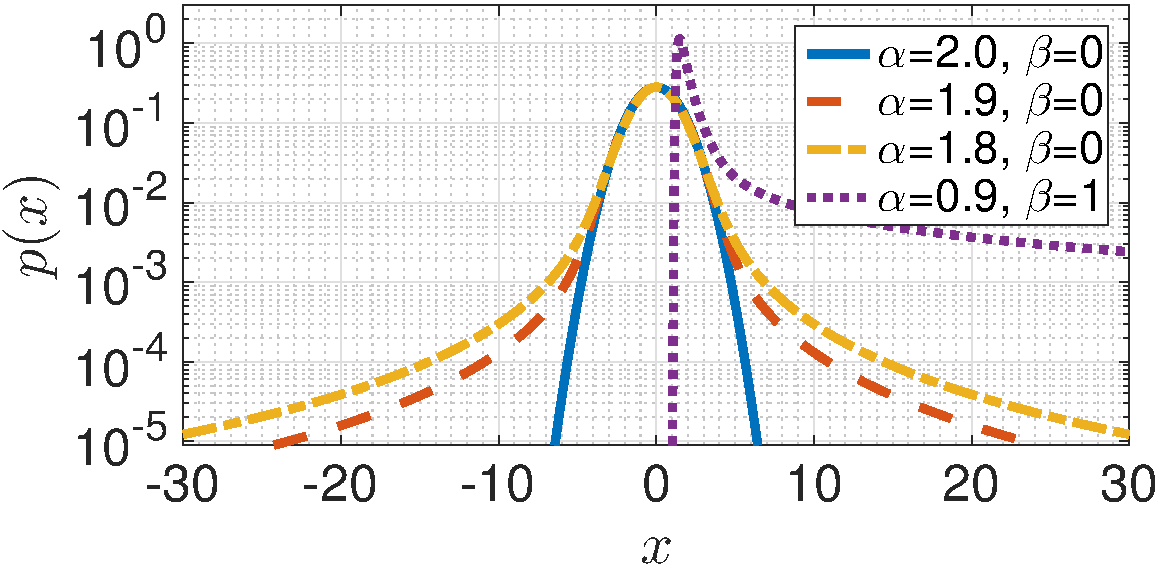
\includegraphics[width=0.31\linewidth]{figures/stablepdf3.pdf}
    \label{fig:stable_pdf}
    } \hfill
    \subfigure[]{
    \includegraphics[width=0.31\linewidth]{figures/cfc_data1_2.pdf}
    \includegraphics[width=0.31\linewidth]{figures/cfc_data2_2.pdf}
    % \includegraphics[width=0.235\linewidth]{figures/lfpdata3.pdf}
    \label{fig:artifacts}
    }
    \caption[PDSFs of $\alpha$-stable distributions and trials containing artifacts.]{(a) PDFs of $\alpha$-stable distributions. (b) Illustration of two trials from the striatal LFP data, which contain severe artifacts. The artifacts are illustrated with dashed rectangles.}
    \label{fig:pdf_lfp}
\end{figure}


% \paragraph{$\alpha$-Stable distributions:}
% \label{sub:stabledist}

% \begin{wrapfigure}{O}{0.5\columnwidth}
% %\vskip 0.2in
% \begin{center}
% % \centerline{
% % \subfigure[]{
% \vspace{-10pt}
% \includegraphics[width=0.49\columnwidth]{./figures/stablepdf.pdf}
% % }
% \end{center}
% \vspace{-15pt}
% \caption{PDFs of stable distributions.}
% \label{fig:stable_pdf} 
% \end{wrapfigure}


\textbf{$\alpha$-Stable distributions:} 
The $\alpha$-stable distributions have become increasingly popular in modeling signals that might incur large variations \citep{kuruoglu1999signal, mandelbrot2013fractals,simsekli2015alpha,wang2016delving,leglaive:hal-01416366} and have a particular importance in statistics since they appear as the limiting distributions in the generalized central limit theorem \citep{samorodnitsky1994stable}. They are characterized by four parameters: $\alpha$, $\beta$, $\sigma$, and $\mu$:
%
(i) $\alpha \in (0,2]$ is the \emph{characteristic exponent} and determines the tail thickness of the distribution: the distribution will be heavier-tailed as $\alpha$ gets smaller. 
(ii) $\beta \in [-1 ,1]$ is the \emph{skewness} parameter.
%and determines whether the distribution is right- or left-skewed
If $\beta = 0$, the distribution is symmetric.
(iii) $\sigma \in (0,\infty)$ is the \emph{scale} parameter and measures the spread of the random variable around its mode (similar to the standard deviation of a Gaussian distribution). Finally, (iv) $\mu \in (-\infty, \infty)$ is the location parameter (for $\alpha > 1$, it is simply the mean). 

The probability density function of an $\alpha$-stable distribution cannot be written in closed-form except for certain special cases; however, the characteristic function  can be written as follows:
%\begin{align*}
%x \sim {\cal S}(\alpha,\beta,\sigma,\mu) \iff \mathds{E}[\exp( i \omega x)]  = \exp(-|\sigma \omega|^\alpha \left[1+ i \sign(\omega)\beta \psi_\alpha(\omega)  \right] + i \mu \omega ) \enspace ,
%\end{align*}
where $\psi_\alpha(\omega) = \log |\omega| $ for $\alpha =1$, $\psi_\alpha(\omega) = \tan(\pi \alpha/2)$ for $\alpha \neq 1$, and $i = \sqrt{-1}$. 
%
As an important special case of the $\alpha$-stable distributions, we obtain the Gaussian distribution when $\alpha = 2$ and $\beta =0$, \textit{i.e.}\ ${\cal S}(2,0,\sigma,\mu) = {\cal N}(\mu,2 \sigma^2)$. 
%
In Fig.~\ref{fig:stable_pdf}, we illustrate the (approximately computed) \acp{PDF} of the $\alpha$-stable distribution for different values of $\alpha$ and $\beta$. The distribution becomes heavier-tailed as we decrease $\alpha$, whereas the tails vanish quickly when $\alpha=2$. 


The moments of the $\alpha$-stable distributions can only be defined up to the order $\alpha$, i.e. $\mathds{E}[|x|^p] < \infty $ if and only if $p <\alpha$, which implies the distribution has infinite variance when $\alpha<2$. Furthermore, despite the fact that the \acp{PDF} of $\alpha$-stable distributions do not admit an analytical form, it is straightforward to draw random samples from them~\citep{chambers1976method}.





\section{Alpha-Stable Convolutional Sparse Coding}

\subsection{The Model}


From a probabilistic perspective, the \ac{CSC} problem can be also formulated as a \ac{MAP} estimation problem on the following probabilistic generative model:
%
\begin{align}
z_{n,t}^k \sim {\cal E}(\lambda),
\quad x_{n,t} | z, d \sim {\cal N}( \hat{x}_{n,t},1 ),
\quad \text{ where,}
\quad \hat{x}_n \triangleq \sum_{k=1}^{K}d^{k} * z_{n}^{k} \enspace .
\label{eqn:csc_prob}
\end{align}
%
Here, $z_{n,t}^k$ denotes the $t$th element of $z_{n}^k$. We use the same notations for $x_{n,t}$ and $\hat{x}_{n,t}$. It is easy to verify that the MAP estimate for this probabilistic model, \textit{i.e.}\ $\max_{d,z} \log p(d,z|x)$, is identical to the original optimization problem defined in~\eqref{eq:problem_definition}\footnote{Note that the positivity constraint on the activations is equivalent to an exponential prior for the regularization term rather than the more common Laplacian prior.}.

It has been long known that, due to their light-tailed nature, Gaussian models often fail at handling noisy high amplitude observations or outliers~\citep{Huber81a}. As a result, the `vanilla' \ac{CSC} model turns out to be highly sensitive to outliers and impulsive noise that frequently occur in electrophysiological recordings, as illustrated in Fig.~\ref{fig:artifacts}. Possible origins of such artifacts are movement, muscle contractions, ocular blinks or electrode contact losses.
 % \umut{Mention the figure from the LFP data.} % albeit it has been shown to be successful for audio processing and computer vision applications.


% In order to be able to handle such challenging data, probabilistic models that are based on non-Gaussian heavy-tailed distributions have become increasingly popular in various domains \umut{should go to intro}. 

% \cite{samoradnitsky1994stable}

In this study, we aim at developing a probabilistic \ac{CSC} model that would be capable of modeling challenging electrophysiological signals. We propose an extension of the original CSC model defined in~\eqref{eqn:csc_prob} by replacing the light-tailed Gaussian likelihood (corresponding to the $\ell_2$ reconstruction loss in~\eqref{eq:problem_definition}) with heavy-tailed $\alpha$-stable distributions. We define the proposed probabilistic model ($\alpha$CSC) as follows:
\begin{align}
z_{n,t}^k \sim {\cal E}( \lambda),  \quad
x_{n,t} | z, d \sim {\cal S} (\alpha, 0, 1/\sqrt{2}, \hat{x}_{n,t} ) \enspace , \label{eqn:acsc_org}
\end{align}
where ${\cal S}$ denotes the $\alpha$-stable distribution.
%
%\footnote{\mainak{We remark here that even though mixture models could also be used to achive robustness, this would most likely be a worse choice compared to alpha stable distributions~\citep{swami2000non}.} \umut{I really don't think these explanations are necessary.}}. 
%
While still being able to capture the temporal structure of the observed signals via convolution, the proposed model has a richer structure and would allow large variations and outliers, thanks to the heavy-tailed $\alpha$-stable distributions. Note that the vanilla \ac{CSC} defined in \eqref{eqn:csc_prob} appears as a special case of $\alpha$CSC, as the $\alpha$-stable distribution coincides with the Gaussian distribution when $\alpha=2$. 


% \mainak{We remark here that even though mixture models could also be used to achive robustness, this would most likely be a worse choice compared to alpha stable distributions~\citep{swami2000non}. Further, even though biconvex problems have theoretical guarantees\citep{agarwal2014learning, gorski2007biconvex}, we observe that in practice, the sampling route does not come with any additional disadvantage due to our multiple restart strategy.} 



%\umut{More explanation on the model, what happens when $\alpha=2$ etc.}




% It is easy to verify that this model coincides with the Gaussian model defined above, when $\alpha=2$. 

\subsection{Maximum A-Posteriori Inference}
%  of the latent variables $d$ and $z$
Given the observed signals $x$, we are interested in the MAP estimates, defined as follows:
\begin{align}
(d^\star,z^\star) = \argmax_{d,z}  \sum_{n,t} \Bigl( \log p(x_{n,t}|d,z) + \sum_k \log p(z_{n,t}^k)  \Bigr).
\end{align}
As opposed to the Gaussian case, unfortunately, this optimization problem is not amenable to classical optimization tools, since the \ac{PDF} of the $\alpha$-stable distributions does not admit an analytical expression.  
%
As a remedy, we use the product property of the symmetric $\alpha$-stable densities \citep{samorodnitsky1994stable,godsill1999bayesian} and re-express the $\alpha$CSC model as conditionally Gaussian. It leads to:
\begin{align}
% z_{i}^k[t] &\sim {\cal E}( \lambda) \\
z_{n,t}^k \sim {\cal E}( \lambda),  \quad 
\phi_{n,t} \sim {\cal S}\Bigl(\frac{\alpha}{2},1, 2 (\cos \frac{\pi \alpha}{4})^{2/\alpha} ,0 \Bigr), \quad
x_{n,t} | z, d, \phi \sim {\cal N}\Bigl(\hat{x}_{n,t},\frac{1}{2}\phi_{n,t} \Bigr) \enspace ,
\label{eqn:sas_condgauss}
\end{align}
where $\phi$ is called the \emph{impulse} variable that is drawn from a \emph{positive} $\alpha$-stable distribution (i.e.\ $\beta =1$), whose \ac{PDF} is illustrated in Fig.~\ref{fig:stable_pdf}. It can be shown that both formulations of the $\alpha$CSC model are identical by marginalizing the joint distribution $p(x,d,z,\phi)$ over $\phi$ \cite[Proposition 1.3.1]{samorodnitsky1994stable}. 

The impulsive structure of the $\alpha$CSC model becomes more prominent in this formulation: the variances of the Gaussian observations are modulated by stable random variables with infinite variance, where the impulsiveness depends on the value of $\alpha$. 
%
It is also worth noting that when $\alpha = 2$, $\phi_{n,t}$ becomes deterministic and we can again verify that $\alpha$CSC coincides with the vanilla \ac{CSC}. 

% One of the main advantages of the augmented model \eqref{eqn:sas_condgauss} is its conditional Gaussianity

The conditionally Gaussian structure of the augmented model has a crucial practical implication: if the impulse variable $\phi$ were to be known, then the \ac{MAP} estimation problem over $d$ and $z$ in this model would turn into a `weighted' \ac{CSC} problem, which is a much easier task compared to the original problem. In order to be able to exploit this property, we propose an \ac{EM} algorithm, which iteratively maximizes a lower bound of the log-posterior $\log p(d,z|x)$, and algorithmically boils down to computing the following steps in an iterative manner:
\begin{align}
&\text{E-Step:} \hspace{20pt} {\cal B}^{(i)}(d,z) = \mathds{E}\left[\log p(x,\phi,z|d)\right]_{p(\phi|x,z^{(i)},d^{(i)})}, \\
&\text{M-Step:} \hspace{20pt} (d^{(i+1)}, z^{(i+1)}) = \argmax\nolimits_{d,z} {\cal B}^{(i)}(d,z). \label{eq:mstep}
\end{align}
where $\mathds{E}[f(x)]_{q(x)}$ denotes the expectation of a function $f$ under the distribution $q$, $i$ denotes the iterations, and ${\cal B}^{(i)}$ is a lower bound to $\log p(d,z|x)$ and it is tight at the current iterates $z^{(i)}$, $d^{(i)}$.



%

%
% Accordingly, the M-Step simplifies as well and becomes:
% %
% \begin{align}
% \min_{d,z\geq 0} \Bigl( \sum_i \sum_t \tau_i[t](x_i[t] -\hat{x}_i[t] )^2 + \lambda \sum_{k}{z_{i}^{k}}    \Bigr).
% \label{eq:mstep}
% \end{align}
% %
% We can observe that the M-step is a slight modification of our initial optimization problem~\eqref{eq:problem_definition}. We now detail computations of both E and M-steps.

% \paragraph{The E-Step:}
\textbf{The E-Step:} 
In the first step of our algorithm, we need to compute the \ac{EM} lower bound ${\cal B}$ that has the following form:
\begin{align}
{\cal B}^{(i)}(d,z) =^+ - \sum_{n=1}^N \Big( \|\sqrt{w_{n}^{(i)}} \odot (x_{n} - \sum_{k=1}^{K}d^{k} * z_{n}^{k})\|_{2}^{2} + \lambda \sum_{k=1}^K{\|z_{n}^{k}\|_1}\Big),
\end{align}
where $=^+$ denotes equality up to additive constants, $\odot$ denotes the Hadamard (element-wise) product, and the square-root operator is also defined element-wise. Here, $w_{n}^{(i)} \in \bbR^T_+$ are the \emph{weights} that are defined as follows: $w_{n,t}^{(i)} \triangleq \mathds{E}\left[1/{\phi_{n,t}}\right]_{p(\phi|x,z^{(i)},d^{(i)})}$. As the variables $\phi_{n,t}$ are expected to be large when $\hat{x}_{n,t}$ cannot explain the observation $x_{n,t}$ -- typically due to a corruption or a high noise -- the weights will accordingly suppress the importance of the particular point $x_{n,t}$. Therefore, the overall approach will be more robust to corrupted data than the Gaussian models where all weights would be deterministic and equal to $0.5$. 

% \utodo{more semantics about this weight.} 

 
%
% \begin{align}
%  \tau_i[t]^{(i)} \triangleq \mathds{E}\left[\frac1{\phi_i[t]}\right]_{p(\phi|x,z^{(i)},d^{(i)})}. \label{eqn:tau_exp}
% \end{align} 

% {% tex broke the page here!!!!
% \parfillskip=0pt
% \parskip=0pt
% \par}

    \begin{algorithm}[H]
      \begin{algorithmic}[1] %(regularization parameter), (number of EM iterations), (number of MCMC iterations)
      \REQUIRE Regularization: $\lambda \in \real_+$, Num. atoms: $K$, Atom length: $L$, Num. iterations: $I$ , $J$, $M$
        %\STATE $\hat{d \in \real^{K \times L}} \leftarrow 0$, $\hat{z} \in \real^{K \times N \times T} \leftarrow 0$
        \FOR{$i=1$ to $I$}
          \STATE \textit{\color{blue} /* E-step: */} %Estimate $w^{(i)}$ as follows:
          \FOR{$j=1$ to $J$}
          \STATE Draw $\phi_{n,t}^{(i,j)}$ via MCMC \eqref{eqn:mcmc_acc}
          \ENDFOR
          \STATE $w_{n,t}^{(i)} \approx (1/J) \sum\nolimits_{j=1}^{J} 1/{\phi_{n,t}^{(i,j)}}$
          % \ENDFOR
          \STATE \textit{\color{blue} /* M-step: */} %Estimate $d^{(i)}, z^{(i)}$ as follows:
              \FOR{$m=1$ to $M$}
                  \STATE $z^{(i)}$ = L-BFGS-B on \eqref{eq:problem_definition_z}
                  \STATE $d^{(i)}$ = L-BFGS-B on the dual of \eqref{eq:problem_definition_d}
              \ENDFOR
        \ENDFOR
        \RETURN $w^{(I)}$, $d^{(I)}$, $z^{(I)}$
        \end{algorithmic}
        \caption{$\alpha$-stable Convolutional Sparse Coding}
        \label{alg:alpha_csc}
    \end{algorithm}

Unfortunately, the weights $w^{(i)}$ cannot be computed analytically, therefore we need to resort to
approximate methods. In this study, we develop a \ac{MCMC} method to approximately compute the weights, where we approximate the intractable expectations with a finite sample average, given as follows: $w_{n,t}^{(i)} \approx (1/{J}) \sum_{j=1}^{J} 1/{\phi_{n,t}^{(i,j)}}$, where $\phi_{n,t}^{(i,j)}$ are some samples that are ideally drawn from the posterior distribution $p(\phi|x,z^{(i)},d^{(i)})$. Unfortunately, directly drawing samples from the posterior distribution of $\phi$ is not tractable either, and therefore, we develop a \emph{Metropolis-Hastings} algorithm \citep{chib1995understanding}, that asymptotically generates samples from the \emph{target} distribution $p(\phi|\cdot)$ in two steps. In the $j$-th iteration of this algorithm, we first draw a random sample for each $n$ and $t$ from the prior distribution (cf.\ \eqref{eqn:sas_condgauss}), \textit{i.e.}, $\phi_{n,t}'\sim p(\phi_{n,t})$. We then compute an acceptance probability for each $\phi_{n,t}'$ that is defined as follows:
%
\begin{align}
  % \text{acc}(\phi_{n,t}^{(i,j)} \rightarrow \phi_{n,t}' ) \triangleq \exp \Bigl\{ (\log \phi_{n,t}^{(i,j)} - \log \phi_{n,t}')/2 + (x_{n,t} - \hat{x}^{(i)}_{n,t})^2 (1/{\phi_{n,t}^{(i,j)}} - 1/{\phi_{n,t}'}) \Bigr\}
  \text{acc}(\phi_{n,t}^{(i,j)} \rightarrow \phi_{n,t}' ) \triangleq \min \Bigl\{1, {p(x_{n,t}|d^{(i)},z^{(i)},\phi'_{n,t})}/{p(x_{n,t}|d^{(i)},z^{(i)},\phi_{n,t}^{(i,j)})} \Bigr\} \label{eqn:mcmc_acc}
\end{align}
%
where $j$ denotes the iteration number of the \ac{MCMC} algorithm. 
% and $\hat{x}^{(i)}_{n}$ is computed as in \eqref{eqn:csc_prob} by using the current iterates $d^{(i)}$ and $z^{(i)}$. 
Finally, we draw a uniform random number $u_{n,t} \sim {\cal U}([0, 1])$ for each $n$ and $t$. If $u_{n,t} < \text{acc}(\phi_{n,t}^{(i)} \rightarrow \phi_{n,t}')$, we accept the sample and set $\phi_{n,t}^{(i+1)} = \phi_{n,t}'$; otherwise we reject the sample and set $\phi_{n,t}^{(i+1)} = \phi_{n,t}^{(i)}$. This procedure forms a Markov chain that leaves the target distribution $p(\phi|\cdot)$ invariant, where under mild ergodicity conditions, it can be shown that the finite-sample averages converge to their true values when $J$ goes to infinity \citep{Liu2008}. More detailed explanation of this procedure is given in Section~\ref{sec:e-step}.

%

%
% \ag{maths / derivations in appendix? it's too fast for me.}
% To simplify notation, from now on, we will use $\tau_{i} \in \bbR^{T}$ to denote all the activations for one sample.
%!TEX root = ../nips_2017.tex



% \paragraph{The M-Step:}
% \label{sec:solve_activation}
\textbf{The M-Step:} 
Given the weights $w_n$ that are estimated during the E-step, the objective of the M-step~\eqref{eq:mstep} is to solve a weighted \ac{CSC} problem, which is much easier when compared to our original problem. 
%
This objective function is not jointly convex in $d$ and $z$, yet it is convex if one fix
either $d$ or $z$.
% Due to non-convexity, we can only guarantee convergence to a local optimum. 
Here, similarly to the vanilla \ac{CSC} approaches~\citep{gips2017discovering,Grosse-etal:2007}, we develop a \emph{block coordinate descent} strategy, where we solve the problem in~\eqref{eq:mstep} for either $d$ or $z$, by keeping respectively $z$ and $d$ fixed.
%
% Since the overall problem is non-convex, one can only aim for obtaining a local optimum. For obtaining a local minimum, several approaches have been proposed \umut{cite}. These methods are based on alternating minimization, where the problem is iteratively solved for either for the atoms while keeping the codes fixed, or vice versa. Both of the two subproblems are convex. \umut{Deficiencies of the algorithms. Algorithms can be made more efficient}
%
% \textbf{Solving for the activations:}
%
We first focus on solving the problem for $z$ while keeping $d$ fixed, given as follows:
\begin{align}
& \min_{z} \sum_{n=1}^{N} \Big( \|\sqrt{w_{n}} \odot (x_{n} - \sum_{k=1}^{K}D^{k} \bar{z}_{n}^{k})\|_{2}^{2} + \lambda \sum_{k}{ \|{z}_{n}^{k} \|_1}\Big) \quad \text{ s.t.  } {z}_n^k \geq 0, \forall n,k\enspace .
\label{eq:problem_definition_z}
\end{align} 
Here, we expressed the convolution of $d^k$ and $z_n^k$ as the inner product of the zero-padded activations $\bar{z}_n^k \triangleq [(z_n^k)^\top, 0 \cdots 0]^\top \in \bbR^{T}_+$, with a Toeplitz matrix $D^k \in \bbR^{T \times T}$, that is constructed from $d^k$.
The matrices $D^k$ are never constructed in practice, and all operations are carried out using convolutions.
This problem can be solved by various constrained optimization algorithms. Here, we choose the quasi-Newton L-BFGS-B algorithm~\cite{byrd1995limited} with a box constraint: $0 \leq z_{n,t}^k \leq \infty$. This approach only requires the simple computation of the gradient of the objective function with respect to $z$ (\textit{cf.} Section~\ref{sec:m-step}). Note that, since trials are mutually independent, we can solve this problem for each $z_n$ in parallel. 

% \subsection{Solving for atoms}
We then solve the problem for the atoms $d$ while keeping $z$ fixed. This optimization problem turns out to be a constrained weighted least-squares problem. In the non-weighted case, this problem can be solved either in the time domain or in the Fourier domain~\citep{Grosse-etal:2007,heide2015fast,wohlberg2016efficient}. The Fourier transform simplifies the convolutions that appear in least-squares problem, but it also induces several difficulties, such as that the atom $d_k$ have to be in a finite support $L$, an important issue ignored in the seminal work of~\cite{Grosse-etal:2007} and addressed with an \ac{ADMM} solver  in \cite{heide2015fast,wohlberg2016efficient}.
In the weighted case, it is not clear how to solve this problem in the Fourier domain. We thus perform all the computations in the time domain.


%The efficiency of the M-step is crucial in our applications, since it will be run several times within a single run of the overall algorithm. Since we will be considering relatively long observations and rather short atoms in our applications, the approaches that operate in the Fourier domain turns out to be inefficient due to the additional constraints that appear only in the frequency domain. Therefore, we perform all the computations in the time domain in order to improve computational efficiency.



% The performances of our strategy will be demonstrated in benchmarks in the next section. for estimating finite impulse response filters  \in \bbR^{T-L+1}
Following the traditional filter identification approach~\citep{moulines1995subspace}, we need to embed the one-dimensional signals $z_n^k$ into a matrix of delayed signals $Z_n^{k} \in \bbR^{T \times L}$, where $ (Z_n^{k})_{i,j} = z_{n,i + j - L + 1}^k$ if $ L - 1 \le i+j < T$ and $0$ elsewhere. Equation~\eqref{eq:problem_definition} then becomes:
%
\begin{align}
& \min_{d} \sum_{n=1}^{N} \|\sqrt{w_n} \odot (x_{n} - \sum_{k=1}^{K}Z_{n}^{k}d^{k})\|_{2}^{2}, \quad \text{  s.t.  } \|d^k\|_2^2 \leq 1 \enspace.
\label{eq:problem_definition_d}
\end{align}
%
Due to the constraint, we must resort to an iterative approach. The options are to use (accelerated) projected gradient methods such as FISTA~\citep{beck2009fast} applied to~\eqref{eq:problem_definition_d}, or to solve a dual problem as done in~\cite{Grosse-etal:2007}. The dual is also a smooth constraint problem yet with a simpler positivity box constraint (\textit{cf.} Section~\ref{sec:m-step}). The dual can therefore be optimized with L-BFGS-B. Using such a quasi-Newton solver turned out to be more efficient than any accelerated first order method in either the primal or the dual (\textit{cf.} benchmarks in Section~\ref{sec:m-step-performance}).
% As in existing literature\cite{}, we first attempted to solve this problem by transforming Equation~\ref{eq:problem_definition} into the frequency domain using a Fourier transform so as to change the convolution into an elementwise multiplication. In fact, this can greatly speed up the computation, but for one crucial fact: truncating the higher order coefficients in the inverse Fourier transform of the estimated atom can make the objective function non-monotonic in the presence of noise. It turns out that the correct approach involves a constraint on the support of the atoms which does not offer similar computational benefits (as will be seen in our Results section).
%




Our entire \ac{EM} approach can be summarized in the Algorithm~\ref{alg:alpha_csc}.
Note that during the alternating minimization, thanks to convexity we can warm start the $d$ update and the $z$ update using the solution from the previous update. This significantly speeds up the convergence of the L-BFGS-B algorithm, particularly in the later iterations of the overall algorithm. We will not describe the E step and the M steps in more detail.

% \mjtodo{We don't talk about warm starting the iterations of EM anywhere. Maybe not very important ...}


\subsection{Details of the E-Step}
\label{sec:e-step}
%\umut{I will put more derivations here.}

Computing the weights that are required in the M-step requires us to compute the expectation of $\frac1{\phi_{n,t}}$ under the posterior distribution $p(\phi_{n,t}|x,d,z)$, which is not analytically available. 

Monte Carlo methods are numerical techniques that can be used to approximately compute the expectations of the form:
\begin{align}
\mathds{E}[f(\phi_{n,t})] = \int f(\phi_{n,t}) \pi(\phi_{n,t}) d\phi_{n,t} \approx \frac1{J} \sum_{j=1}^J f(\phi_{n,t}^{(j)}) \label{eqn:mc}
\end{align}
where $\phi_{n,t}^{(j)}$ are some samples drawn from $\pi(\phi_{n,t}) \triangleq p(\phi_{n,t}|x,d,z)$ and $f(\phi) = 1/\phi$ in our case. However, in our case, sampling directly from $\pi(\phi_{n,t})$ is also unfortunately intractable.

%  through a transition kernel;  $ \mathbf{\Theta}^{(i+1)} \sim {\cal T}(\mathbf{\Theta}|\mathbf{\Theta}^{(i)})$

\ac{MCMC} methods generate samples from the target distribution $\pi(\phi_{n,t})$ by forming a Markov chain, whose stationary distribution is $\pi(\phi_{n,t})$, 
%
so that $\pi(\phi_{n,t}) = \int {\cal T}(\phi_{n,t}|\phi_{n,t}') p(\phi_{n,t}') d\phi_{n,t}'$, where ${\cal T}$ denotes the transition kernel of the Markov chain. 

In this study, we develop a \ac{MH} algorithm, that implicitly forms a transition kernel. 
%
The MH algorithm generates samples from a target distribution $\pi(\phi_{n,t})$ in two steps. First, it generates a random sample $\phi_{n,t}'$ from a \emph{proposal} distribution $\phi_{n,t}' \sim q(\phi_{n,t}'|\phi_{n,t}^{(j)})$, then computes an acceptance probability $\text{acc}(\phi_{n,t}^{(j)} \rightarrow \phi_{n,t}')$ and draws a uniform random number $u \sim {\cal U}([0, 1])$. If $u < \text{acc}(\phi_{n,t}^{(j)} \rightarrow \phi_{n,t}')$, it accepts the sample and sets $\phi_{n,t}^{(j+1)} = \phi_{n,t}'$; otherwise it rejects the sample and sets $\phi_{n,t}^{(j+1)} = \phi_{n,t}^{(j)}$. The acceptance probability is given as follows
\begin{align}
\text{acc}(\phi_{n,t} \rightarrow \phi_{n,t}') 
&= \min \Bigr\{1, \frac{q(\phi_{n,t}|\phi_{n,t}') \pi(\phi_{n,t}')}{q(\phi_{n,t}'|\phi_{n,t}) \pi(\phi_{n,t})}\Bigr\} \nonumber \\
&= \min \Bigr\{1, \frac{q(\phi_{n,t}|\phi_{n,t}') p(x_{n,t}|\phi_{n,t}',d,z) p(\phi_{n,t}') }{q(\phi_{n,t}'|\phi_{n,t}) p(x_{n,t}|\phi_{n,t},d,z) p(\phi_{n,t}) }\Bigr\}
\end{align}
where the last equality is obtained by applying the Bayes rule on $\pi$. 

The acceptance probability requires the prior distribution of $\phi$ to be evaluated. Unfortunately, this is intractable in our case since this prior distribution is chosen to be a positive $\alpha$-stable distribution whose PDF does not have an analytical form. As a remedy, we choose the prior distribution of $\phi_{n,t}$ as the proposal distribution, such $q(\phi_{n,t}|\phi_{n,t}') = p(\phi_{n,t})$. This enables us to simplify the acceptance probability. Accordingly, for each $\phi_{n,t}$, we have the following acceptance probability:
\begin{align}
  \text{acc}(\phi_{n,t}^{(i,j)} \rightarrow \phi_{n,t}' ) \triangleq \min  \Bigl\{1, \exp(\log \phi_{n,t}^{(i,j)} - \log \phi_{n,t}')/2 + (x_{n,t} - \hat{x}^{(i)}_{n,t})^2 (1/{\phi_{n,t}^{(i,j)}} - 1/{\phi_{n,t}'}) \Bigr\}.
\end{align}
Thanks to the simplification, this probability is tractable and can be easily computed. 

\subsection{Details of the M-Step}
\label{sec:m-step}
\paragraph{Solving for the activations: }
In the M-step, we optimize~\eqref{eq:problem_definition_z} to find the activations $z_n^{(i)}$ of each trial $n$ independently. To keep the notation simple, we will drop the index for the iteration number $i$ of the EM algorithm.

First, this equation can be rewritten by concatenating the Toeplitz matrices for the $K$ atoms into a big matrix $D = [D^1, D^2, ..., D^K] \in \bbR^{T \times KT}$ and the activations for different atoms into a single vector $\bar{z}_n = [(\bar{z}_n^1)^\top, (\bar{z}_n^2)^\top, ..., (\bar{z}_n^K)^\top]^\top \in \bbR^{KT}_+$ where $(\cdot)^\top$ denotes the transposition operation. Recall that $\bar{z}_n^k$ is a zero-padded version of $z_n^k$. This leads to a simpler formulation and the objective function $\mathcal{L}(d, z)$:
\begin{equation}
\mathcal{L}(d, z) = \sum_{n=1}^{N} \frac{1}{2}\|\sqrt{w_{n}} \odot (x_{n} - D \bar{z}_{n})\|_{2}^{2} + \lambda \mathbbm{1}^\top \bar{z}_{n} \enspace ,
\label{eq:problem_definition_d_simple}
\end{equation}
where $\mathbbm{1} \in \bbR^{KT}$ is a vector of ones.

The derivative w.r.t. $z_n$ now reads:
\begin{equation}
\frac{\partial \mathcal{L}(d, z)}{\partial \bar{z}_n}
= D^\top(w_n \odot (x_n - D\bar{z}_n)) + \lambda \mathbbm{1}^\top \enspace .
\end{equation}
In practice, this big matrix $D$ is never assembled and all operations are carried out using convolutions. Note also that we do not update the zeros from the padding in $\bar{z}_n^k$. Now that we have the gradient, the activations can be estimated using a efficient quasi-Newton solver such as L-BFGS-B, taking into account the box posititivy constraint $0 \leq z_n \leq \infty$.
%In the case of PG algorithm, one has a modified soft thresholding operator given by a rectified linear function $\mathcal{S}_{\lambda t}=\mathrm{max}(0, z_i - \lambda t)$.
%The step size for ISTA and FISTA can be chosen to be the inverse of the Lipschitz constant which is equal to the largest eigenvalue of $D^{\top}(\tau_{i} \odot D)$. In practice, this is estimated using the power iteration method \mainak{[ref]} with warm restarts.

For each trial, one iteration costs $\mathcal{O}(LKT)$.

\paragraph{Solving for the atoms: }

In the M-step, we optimize \eqref{eq:problem_definition_d} to find the atoms $d^k$.
As when solving for the activations $z_n$, we can remove the summation over the atoms by concatenating the delayed matrices into $Z_{n}=[Z_{n}^1, Z_{n}^2, \dots, Z_{n}^K] \in \bbR^{T \times KL}$ and $d=[(d^1)^\top, (d^2)^\top, ..., (d^K)^\top]^\top \in \bbR^{KL}$. This leads to the simpler formulation:
%
\begin{align}
& \min_{d} \sum_{n=1}^{N} \frac{1}{2}\|\sqrt{w_n} \odot (x_{n} - Z_{n}d)\|_{2}^{2}, \quad \text{  s.t.  } \|d^k\|_2^2 \leq 1 \enspace.
\label{eq:subproblem_d}
\end{align}
%
%If not for the constraint, this is a classic least square problem which has a known closed-form solution:
%\begin{equation}
%\hat{d} = \Big(\sum_{i=1}^N Z_i^{\top}(\tau_{i} \odot Z_i) \Big)^{-1}\sum_{i=1}^{N} (\tau_{i} \odot Z_i)^{\top}x_i
%\end{equation}
%\ag{say somewhere that FFT based cross-correlation is not possible anymore with EM sample weights}
%\ag{we need to keep the maths for what we are doing and put all the rest in appendix. No need to remind text book notions of optim in main text.}
%
 The Lagrangian of this problem is given by:
%
\begin{equation}
g(d, \beta) = \sum_{n=1}^{N} \frac{1}{2}\|\sqrt{w_n} \odot (x_{n} - \sum_{k=1}^{K} Z_{n}^{k}d^{k}) \|_{2}^{2} + \sum_k \beta^k (\|d^k\|_2^{2} - 1) \quad \text{s.t. } \beta^k \geq 0 \enspace,
\end{equation}
%
where $\beta = (\beta^1, \beta^2, ..., \beta^K)$ are the dual variables. Therefore, the dual problem is:
%
\begin{align}
\min_{d}{g(d, \beta)} = g(d^{*}, \beta)
\end{align}
%
where $d^*$, the primal optimal, is given by:
%
\begin{equation}
d^{*} = (\sum_{n=1}^N Z_n^{\top}(w_{n} \odot Z_n) + \bar{\beta} )^{-1}\sum_{n=1}^{N}(w_{n} \odot Z_n)^{\top}x_n
\label{eq:dual_optimal}
\end{equation}
%
with $\bar{\beta} = \mathrm{diag}([\mathbbm{1}\beta^1, \mathbbm{1}\beta^2, ..., \mathbbm{1}\beta^K]) \in \bbR^{KL}$ with $\mathbbm{1} \in \bbR^{L}$. The gradient for the dual variable $\beta^k$ is given by:
%
\begin{equation}
\frac{\partial g(d^{*}, \beta)}{\partial \beta^k}  = \|{d^{*}}^k\|_2^2 - 1,
\end{equation}
%
with ${d^{*}}^k$ computed from~\eqref{eq:dual_optimal}.
%Of course, we do not know the primal optimal $\hat{d}^k$ offhand, as it is what we want to estimate.
We can solve this iteratively using again L-BFGS-B taking into account the positivity constraint $\beta^k \geq 0$ for all $k$.
% It amounts to computing the primal update at each step, then the dual gradients according to the updated primal, then updating the dual using the gradient and continuing this way until convergence. \mainak{Is there a name for this class of algorithms, so the reader can easily relate?}
What we have described so far solves for all the atoms simultaneously. However, it is also possible to estimate the atoms sequentially one at a time using a block coordinate descent (BCD) approach, as in the work of \citep{mairal2010online}. In each iteration of the BCD algorithm, a residual $r_n^k$ is computed as given by:
%
\begin{equation}
r_n^k = x_n - \sum_{k'\neq k} Z^{k'}_{n}d^{k'}
\end{equation}
%
and correspondingly subproblem \ref{eq:subproblem_d} becomes:
%
\begin{align}
& \min_{d^k} \sum_{n=1}^{N} \frac{1}{2}\|\sqrt{w_n} \odot (r^k_{n} - Z^k_{n}d^k)\|_{2}^{2}, \quad \text{  s.t.  } \|d^k\|_2^2 \leq 1, \enspace.
\label{eq:subproblem_d_block}
\end{align}
%
%Solving for atoms can be done all atoms simultaneously or using a block coordinate descent approach by looping sequentially over atoms.
which is solved in the same way as subproblem~\ref{eq:subproblem_d}. Now, in the simultaneous case, we construct one linear problem in $\mathcal{O}(L^2K^2TN)$ and one iteration costs $\mathcal{O}(L^3K^3)$. However, in the BCD strategy, we construct $K$ linear problems in $\mathcal{O}(L^2TN)$ and one iteration costs only $\mathcal{O}(L^3)$.
Interestingly, when the weights $w_n$ are all identical, we can 
use the fact that for one atom $k$, the matrix $\sum_{i=1}^{N}(Z_i^k)^T Z_i^k$ is Toeplitz. In this case, we can construct $K$ linear problems in only $\mathcal{O}(LTN)$ and one iteration costs only $\mathcal{O}(L^2)$.

For the benefit of the reader, we summarize the complexity of the M-step in Table~\ref{table:complexity_m}. We note $p$ and $q$ the number of iterations in the L-BFGS-B methods for the activations update and atoms update.


% \subsection{Computational tricks and complexity analysis}
\begin{table}[htb]
\begin{center}
\begin{tabular}{|l|l|}
\hline
Method & Complexity \\
\hline
Solving activations $z$ & $p\min(L, \log(T))KTN$ \\
%\hline
%z update LBFGS-B & $\min(pLKTN, p\log(T)KTN)$ \\
%\hline
%d update primal & $L^2K^2TN + qL^2K^2$ \\
%\hline
Solving atoms $d$ & $L^2K^2TN + qL^3K^3$ \\
%\hline
%d update block primal & $LKTN + qL^2K$ \\
%\hline
Solving atoms $d$ (sequential) & $LKTN + qL^2K$ \\
\hline
\end{tabular}
\vspace{5pt}
\caption[Complexity analysis of the M-step.]{Complexity analysis of the M-step, where $p$ and $q$ are the number of iterations in the L-BFGS-B solvers for the activations and atoms updates.}
\label{table:complexity_m}
\end{center}
\end{table}






%!TEX root = ../nips_2017.tex


\begin{figure}[t]
    \centering
     \subfigure[$K=10$, $L=32$.]{
     \includegraphics[width=0.30\linewidth]{figures/relative_10_32.pdf}}
     \subfigure[Time to reach a relative precision of 0.01.]{
     \includegraphics[width=0.67\textwidth]{figures/bar_plot.pdf}}
    \caption[Comparison of state-of-the-art methods with our approach.]{Comparison of state-of-the-art methods with our approach. (a)~Convergence plot with the objective function relative to the obtained minimum, as a function of computational time. (b)~Time taken to reach a relative precision of $10^{-2}$, for different settings of $K$ and $L$.  }
    \label{fig:convergence}
\end{figure}

\section{Experiments}
\label{sec:experiments}
In order to evaluate our approach, we conduct several experiments on both synthetic and real data. 
First, we show that our proposed optimization scheme for the M-step provides significant improvements in terms
of convergence speed over the state-of-the-art CSC methods. Then, we provide empirical evidence that our algorithm is more robust to
artifacts and outliers than three competing CSC methods~\citep{jost2006motif,brockmeier2016learning,wohlberg2016efficient}.
%
Finally, we consider LFP data, where we illustrate that our algorithm can reveal interesting properties in electrophysiological signals
without supervision, even in the presence of severe artifacts. The source code is publicly available at \url{https://alphacsc.github.io/}.


% We then show that our algorithmic strategy based on temporal convolutions
% and L-BFGS-B for the M-step outperforms state-of-the-art solvers in terms
% of convergence speed. 



% \paragraph{Synthetic simulation setup:}
\textbf{Synthetic simulation setup:} 
In our synthetic data experiments, we simulate $N$ trials of length $T$ by first generating $K$ zero mean and unit norm atoms of length $L$. The  activation instants are integers drawn from a uniform distribution in $\llbracket0, T-L \rrbracket$. The amplitude of the activations are drawn from a uniform distribution in $[0, 1]$. Atoms are activated only once per trial and are allowed to overlap. The activations are then convolved with the generated atoms and summed up as in \eqref{eq:problem_definition}. 


% \paragraph{M-step performance:}
\subsection{M-step performance} 
\label{sec:m-step-performance}
In our first set of synthetic experiments, we illustrate the benefits of our M-step optimization approach over state-of-the-art CSC solvers. 
%
%Besides existing CSC solvers cannot be directly applied to the M-step of our algorithm for $\alpha < 2$, even in the case where $\alpha=2$ they turn out to be not as efficient when applied to neural signals, since they solve the problem in the Fourier domain which introduces additional projection operations. 
%
We set $N=100$, $T=2000$ and $\lambda=1$, and use different values for $K$ and $L$. To be comparable, we set $\alpha=2$ and add Gaussian noise to the synthesized signals, where the standard deviation is set to $0.01$. In this setting, we  have $w_{n,t}=1/2$ for all $n$, $t$, which reduces the problem to a standard CSC setup. We monitor the convergence of ADMM-based methods by \citet{heide2015fast} and \citet{wohlberg2016efficient} against our M-step algorithm, using both a single-threaded and a parallel version for the $z$-update. 
% We used here artifact-free data. 
As the problem is non-convex, even if two algorithms start from the same point, they are not guaranteed to reach the same local minimum\footnote{Note that the M-step can be viewed as a biconvex problem, for which global convergence guarantees can be shown under certain assumptions \citep{agarwal2014learning, gorski2007biconvex}. However, we have observed that it is required to use multiple restarts even for vanilla CSC, implying that these assumptions are not satisfied in this particular problem.}. 
%
Hence, for a fair comparison, we use a multiple restart strategy with averaging across $24$ random seeds.




 % we observe that in practice, the sampling route does not come with any additional disadvantage due to our multiple restart strategy.

% It is true that the vanilla CSC can be viewed as a biconvex problem with guarantees for convergence to the global minimum under some assumptions (e.g., Agarwal et al, 2014; Gorski et al, 2007). However, we observe in practice that these assumptions are not satisfied, which is why we need to use multiple restarts even for vanilla CSC. Therefore, in introducing an EM loop, we do not sacrifice such convergence properties.

% the d-updates for

During our experiments we have observed that the ADMM-based methods do not guarantee the feasibility of the iterates. In other words, the norms of the estimated atoms might be greater than $1$ during the iterations. To keep the algorithms comparable, when computing the objective value, we project the atoms to the unit ball and scale the activations accordingly. To be strictly comparable, we also imposed a positivity constraint on these algorithms. This is easily done by modifying the soft-thresholding operator to be a rectified linear function. In the benchmarks, all algorithms use a single thread, except ``M-step - 4 parallel'' which uses 4 threads during the $z$ update.

In Fig.~\ref{fig:convergence}, we illustrate the convergence behaviors of the different methods.
%Note that the y-axis is the relative precision with respect to the best obtainable objective function value upon convergence for the local minima that the algorithm converges to. % nice one !
Note that the y-axis is the precision relative to the objective value obtained upon convergence. In other words, each curve is relative to its own local minimum (see next paragraph for details).
In the right subplot, we show how long it takes for the algorithms to reach a relative precision of $0.01$ for different settings (\textit{cf.} next paragraph for more benchmarks). Our method consistently performs better and the difference is even more striking for more challenging setups. This speed improvement on the M-step is crucial for us as this step will be repeatedly executed. % in the EM algorithm. 
%This sets the stage for us to apply $\alpha$CSC on datasets of realistic dimensions.
%
%
%
%%%%%%%%%%%%%%%%%%%%%%%%%%%%%%%%%%%%%%%%%%%%%%%%%%%%%%%%%%%%%%%
%%%%%%%%%%%%%%%%%%%%%%%%%%%%%%%%%%%%%%%%%%%%%%%%%%%%%%%%%%%%%%%
%
% \paragraph{Robustness against corrupted data:}
%

\paragraph{Convergence plots:}

\begin{figure}[htb]
    \centering
     \subfigure[$K=2$, $L=32$.]{
     \includegraphics[width=0.31\linewidth]{figures/relative_2_32.pdf}}
     \subfigure[$K=2$, $L=128$.]{
     \includegraphics[width=0.31\textwidth]{figures/relative_2_128.pdf}}
     \subfigure[$K=10$, $L=32$.]{
     \includegraphics[width=0.31\textwidth]{figures/relative_10_32.pdf}}
    \caption[Convergence speed of the relative objective function.]{Convergence speed of the relative objective function. The y-axis shows the objective function relative to the obtained minimum for each run: $(f(x) - f(x^*))/f(x^*)$. Each curve is the geometrical mean over 24 different random initializations.}
    \label{fig:convergence_setups}
\end{figure}

Here, we compare convergence plots of our algorithm against a number of state-of-art methods. Fig.~\ref{fig:convergence_setups} demonstrates on a variety of setups the computational
advantage of our quasi-Newton approach to solve the M-step.
Note that Fig.~\ref{fig:convergence}b is in fact a summary of Fig.~\ref{fig:convergence_setups}. 
Indeed, we can verify that ADMM methods converge quickly to a modest accuracy, but take much longer to converge to a high accuracy~\citep{boyd2011distributed}.

Next, in Fig.~\ref{fig:convergence_traditional}, we show more traditional convergence plots. In contrast to Fig.~\ref{fig:convergence} or \ref{fig:convergence_setups} where the relative objective function is shown, here we plot the absolute value of the objective function. We can now verify that each of the methods have indeed converged to their respective local minimum. Of course, owing to the non-convex nature of the problem, they do not necessarily converge to the same local minimum.
\begin{figure}[htb]
    \centering
     \subfigure[$K=2$, $L=32$.]{
     \includegraphics[width=0.31\linewidth]{figures/plateau_2_32.pdf}}
     \subfigure[$K=2$, $L=128$.]{
     \includegraphics[width=0.31\textwidth]{figures/plateau_2_128.pdf}}
     \subfigure[$K=10$, $L=32$.]{
     \includegraphics[width=0.31\textwidth]{figures/plateau_10_32.pdf}}
    \caption[Convergence of the objective function as a function of time.]{Convergence of the objective function as a function of time. The y-axis shows the absolute objective function $f(x)$. Each curve is the mean over 24 different random initializations.}
    \label{fig:convergence_traditional}
\end{figure}

\paragraph{Comparison of solver for the activations subproblem:}

Finally, we compare convergence plots of our algorithm using different solvers for the $z$-update: ISTA, FISTA, and L-BFGS-B. The rationale for choosing a quasi-Newton solver for the $z$-update becomes clear in  Fig.~\ref{fig:convergence_z_update} as the L-BFGS-B solver turns out to be computationally advantageous on a variety of setups.

\begin{figure}[h]
    \centering
     \subfigure[$K=2$, $L=32$.]{
     \includegraphics[width=0.31\linewidth]{figures/fista_2_32.pdf}}
     \subfigure[$K=2$, $L=128$.]{
     \includegraphics[width=0.31\textwidth]{figures/fista_2_128.pdf}}
     \subfigure[$K=10$, $L=32$.]{
     \includegraphics[width=0.31\textwidth]{figures/fista_10_32.pdf}}
    \caption[Comparison of solvers for the activations subproblem.]{Convergence speed of the relative objective function. The y-axis shows the objective function relative to the obtained minimum for each run: $(f(x) - f(x^*))/f(x^*)$. Each curve is the geometrical mean over 24 different random initializations.}
    \label{fig:convergence_z_update}
\end{figure}

\subsection{Robustness to corrupted data} 

\newcommand{\tmpsize}{0.15}
\begin{figure}[t]
%\vskip 0.2in
\begin{center}
\subfigure[No corruption.]{
 \setlength{\tabcolsep}{0.5pt} 
    \begin{tabular}{c c}

        \includegraphics[width=\tmpsize\linewidth]{figures/synth_1_rnn_v2.pdf} &
        \includegraphics[width=\tmpsize\linewidth]{figures/synth_1_motif_v2.pdf}
        \\
        \includegraphics[width=\tmpsize\linewidth]{figures/synth_1_1_v2.pdf} &
        \includegraphics[width=\tmpsize\linewidth]{figures/synth_1_2_v2.pdf}
        \end{tabular}
} \hfill
\subfigure[10\% corruption. ]{
\setlength{\tabcolsep}{0.5pt} 
\begin{tabular}{c c}
        \includegraphics[width=\tmpsize\linewidth]{figures/synth_2_rnn_v2.pdf} &
        \includegraphics[width=\tmpsize\linewidth]{figures/synth_2_motif_v2.pdf}
\\
        \includegraphics[width=\tmpsize\linewidth]{figures/synth_2_1_v2.pdf} &
        \includegraphics[width=\tmpsize\linewidth]{figures/synth_2_2_v2.pdf}
        \end{tabular}
}\hfill
\subfigure[20\% corruption]{
\setlength{\tabcolsep}{0.5pt} 
\begin{tabular}{c c}
    \includegraphics[width=\tmpsize\linewidth]{figures/synth_3_rnn_v2.pdf} & 
    \includegraphics[width=\tmpsize\linewidth]{figures/synth_3_motif_v2.pdf}\\
%
    \includegraphics[width=\tmpsize\linewidth]{figures/synth_3_1_v2.pdf}&
    \includegraphics[width=\tmpsize\linewidth]{figures/synth_3_2_v2.pdf}
    \end{tabular}
}
\end{center}
\caption[Simulation to compare state-of-the-art methods against $\alpha$CSC.]{Simulation to compare state-of-the-art methods against $\alpha$CSC.}
\label{fig:mcem_simulated}
\end{figure}

In our second synthetic data experiment, we illustrate the robustness of $\alpha$CSC in the presence of corrupted observations.
%
In order to simulate the likely presence of high amplitude artifacts, one way would be to directly simulate the generative model in \eqref{eqn:acsc_org}. However, this would give us an unfair advantage, since $\alpha$CSC is specifically designed for such data. Here, we take an alternative approach, where we corrupt a randomly chosen fraction of the trials ($10\%$ or $20\%$) with strong Gaussian noise of standard deviation $0.1$, \textit{i.e.} one order of magnitude higher than in a regular trial. We used a regularization parameter of $\lambda = 0.1$.
%
In these experiments, by CSC we refer to $\alpha$CSC with $\alpha=2$, that resembles using only the M-step of our algorithm with deterministic weights $w_{n,t}=1/2$ for all $n$, $t$. We used a simpler setup where we set $N=100$, $T=512$, and $L=64$. We used $K=2$ atoms, as shown in dashed lines in Fig.~\ref{fig:mcem_simulated}.

% We test the standard CSC and $\alpha$CSC algorithms on the simulated data corrupted with artifacts.
%
 %~\footnote{For the CSC model it matches atoms that lead to the smallest values of the objective.}.

% The reader may have already noticed that computing this is not possible when working with real data because the true atoms are not known. Indeed, when multiple restarts are involved, the best restart can be chosen only if one is minimizing a well-defined cost function.
%
For $\alpha$CSC, we set the number of outer iterations $I=5$, the number of iterations of the M-step to $M=50$, and the number of iterations of the MCMC algorithm to $J=10$. We discard the first $5$ samples of the MCMC algorithm as burn-in.
%
% We set $I=5$ iterations of the EM algorithm in $\alpha$CSC and , starting with the M-step and ending with the M-step. The MCMC algorithm was run for 10 iterations with the first 5 iterations being discarded for computing the expectation. 
%
To enable a fair comparison, we run the standard CSC algorithm for $I\times M$ iterations, i.e.\ the \emph{total} number of M-step iterations in $\alpha$CSC. We also compared $\alpha$CSC against competing state-of-art methods previously applied to neural time series: \citet{brockmeier2016learning} and MoTIF~\citep{jost2006motif}. 
%
Starting from multiple random initializations, the estimated atoms with the smallest $\ell_2$ distance with the true atoms are shown in Fig.~\ref{fig:mcem_simulated}.

% The learned atoms are shown in Fig.~\ref{fig:mcem_simulated}. 

\begin{figure}[b]
    \centering
             \subfigure[LFP spike data from \cite{hitziger2017adaptive}]{
             \includegraphics[height=3cm]{figures/spike_atomsa.pdf}
             \label{fig:spikedata}}
             \subfigure[Estimated atoms]{
             \includegraphics[height=2.9cm]{figures/spike_atomsb.pdf}
             \label{fig:spikeatoms}}

            \caption[Atoms learnt by $\alpha$CSC on LFP data containing epileptiform spikes with $\alpha=2$.]{Atoms learnt by $\alpha$CSC on LFP data containing epileptiform spikes with $\alpha=2$.}
\end{figure}

In the artifact-free scenario, all algorithms perform equally well, except for MoTIF that suffers from the presence of activations with varying amplitudes. This is because it aligns the data using correlations before performing the eigenvalue decomposition, without taking into account the strength of activations in each trial. The performance of \citet{brockmeier2016learning} and CSC degrades as the level of corruption increases. On the other hand, $\alpha$CSC is clearly more robust to the increasing level of corruption and recovers reasonable atoms even when 20\% of the trials are corrupted. 



% $\alpha$CSC learned good atoms even on corrupted data.

\subsection{Results on LFP data}
In our last set of experiments, we consider real neural data from two different datasets. 
%
We first applied $\alpha$CSC on an LFP dataset previously used in~\cite{hitziger2017adaptive} and containing epileptiform spikes as shown in Fig.~\ref{fig:spikedata}. The data was recorded in the rat cortex, and  is free of artifact. Therefore, we used the standard CSC with our optimization scheme, (i.e.\ $\alpha$CSC with $\alpha=2$).
%
As a standard preprocessing procedure, we applied a high-pass filter at $1$\,Hz in order to remove drifts in the signal, and then applied a tapered cosine window to down-weight the samples near the edges. We set $\lambda=6$, $N=300$, $T=2500$, $L=350$, and $K=3$. The recovered atoms by our algorithm are shown in Fig.~\ref{fig:spikeatoms}. We can observe that the estimated atoms resemble the spikes in Fig.~\ref{fig:spikedata}. These results show that, without using any heuristics, our approach can recover similar atoms to the ones reported in \cite{hitziger2017adaptive}, even though it does not make any assumptions on the shapes of the waveforms, or initializes the atoms with template spikes in order to ease the optimization.


% Interpreting these atoms is not so straightforward, however it is easy to verify visually these atoms resemble the spikes in Fig.~\ref{fig:spikedata}.



The second dataset is an LFP channel in a rodent striatum from~\cite{dallerac2017updating}. We segmented the data into $70$ trials of length $2500$ samples, windowed each trial with a tapered cosine function, and detrended the data with a high-pass filter at $1$\,Hz.
 % to downweight the effect of samples near the edges, which cannot be handled gracefully by the convolutions. 
We set $\lambda=10$, initialized the weights $w_n$ to the inverse of the variance of the trial $x_n$. Atoms are in all experiments initialized with Gaussian white noise.


% We compared $\alpha$CSC against CSC on artifact-free data and on data corrupted by strong artifacts (see Fig.~\ref{fig:pdf_lfp}). 

As opposed to the first LFP dataset, this dataset contains strong artifacts, as shown in Fig.~\ref{fig:artifacts}. In order to be able to illustrate the potential of CSC on this data, we first \emph{manually} identified and removed the trials that were corrupted by artifacts. In Fig.~\ref{fig:rat3atoms}, we illustrate the estimated atoms with CSC on the manually-cleaned data. We observe that the estimated atoms correspond to canonical waveforms found in the signal. In particular, the high frequency oscillations around $80$\,Hz are modulated in amplitude by the low-frequency oscillation around $3$\,Hz, a phenomenon known as \ac{CFC}~\citep{jensen2007cross}. We can observe this by computing a comodulogram~\citep{tort2010measuring} on the entire signal (Fig.~\ref{fig:comodulogram}). This measures the correlation between the amplitude of the high frequency band and the phase of the low frequency band. 


Even though CSC is able to provide these excellent results on the cleaned data set, its performance heavily relies on the manual removal of the artifacts. Finally, we repeated the previous experiment on the full data, without removing the artifacts and compared CSC with $\alpha$CSC, where we set $\alpha=1.2$. The results are shown in the middle and the right sub-figures of Fig.~\ref{fig:rat3atoms}. It can be observed that in the presence of strong artifacts, CSC is not able to recover the atoms anymore. On the contrary, we observe that $\alpha$CSC can still recover atoms as observed in the artifact-free regime. In particular, the cross-frequency coupling phenomenon is still visible.


\begin{figure}[htb]
    \centering
    \subfigure[Atoms learnt by: CSC (clean data), CSC (full data), $\alpha$CSC (full data)]{
    \includegraphics[width=0.65\linewidth]{figures/rat3atoms.pdf}
    \label{fig:rat3atoms}
    }
    \subfigure[Comodulogram.]{
    \includegraphics[width=0.28\linewidth]{figures/comodulogram.pdf}
    \label{fig:comodulogram}
    }
    \caption[Three atoms learnt from a rodent striatal LFP channel, using CSC on cleaned data, and both CSC and $\alpha$CSC on the full data.]{(a)~Three atoms learnt from a rodent striatal LFP channel, using CSC on cleaned data, and both CSC and $\alpha$CSC on the full data. The atoms capture the cross-frequency coupling of the data (dashed rectangle). (b)~Comodulogram presents the cross-frequency coupling intensity computed between pairs of frequency bands on the entire cleaned signal, following \cite{tort2010measuring}.}
    \label{fig:ratdata}
\end{figure}


  % However, when the data contains heavy artifacts, . Indeed, to recover the prototypical atoms in the presence of artifacts, we must use $\alpha$CSC as shown in the last subplot of .

%) are good when the data is artifact-free, but are strongly affected by the artifacts. On the contrary, the atoms learned with $\alpha$CSC are also good on corrupted data. Interestingly, we are able to recover from the data not only the triangular shaped oscillation, but also the \emph{cross-frequency coupling}. Indeed, in this signal, the high frequency oscillations around 80\,Hz are modulated in amplitude by the low-frequency oscillation around 3\,Hz.
%To visualize this cross-frequency coupling, we computed a comodulogram on the entire signal (Fig.~\ref{fig:comodulogram}). For each pairs of frequency bands, it quantifies the correlation between the amplitude of the high frequency and the phase of the low frequency, following the method from \cite{tort2010measuring}.
%The three atoms all capture this cross-frequency coupling, and show different canonical shapes for the signal.


%!TEX root = ../nips_2017.tex

\section{Conclusion}
\label{sec:alphacsc_conclusion}
% This work addresses the present need in the neuroscience community to better capture the complex morphology of brain waves~\cite{cole2017brain, gips2017discovering}. Our data-driven approach to this problem is a probabilistic formulation of a convolutional sparse coding model~\cite{Grosse-etal:2007}. We propose an inference strategy based on Monte Carlo EM to deal efficiently with heavy tailed noise and take into account the polarity of neural activations with a positivity constraint. Our problem formulation allows the use of fast quasi-Newton methods for the M-step which outperform previously proposed state-of-the-art ADMM-based algorithms~\cite{heide2015fast,wohlberg2016efficient,wohlberg2014efficient,bristow2013fast}, even when not making use of our parallel implementation. Results on LFP data demonstrate that such algorithms can be robust to the presence of transient artifacts in data and reveal insights on neural time-series without supervision.
% \umut{Our code is publicly available.}

\vspace{-5pt}

We address the present need in the neuroscience community to better capture the complex morphology of brain waves. Our approach is based on a probabilistic formulation of a CSC model. We propose an inference strategy based on MCEM to deal efficiently with heavy tailed noise and take into account the polarity of neural activations with a positivity constraint. Our problem formulation allows the use of fast quasi-Newton methods that outperform previously proposed state-of-the-art ADMM-based algorithms, even when not making use of our parallel implementation. Results on LFP data demonstrate that such algorithms can be robust to the presence of transient artifacts in data and reveal insights on neural time-series without supervision.

\acresetall % reset acronyms for conclusion
\chapter{Conclusion}
\label{chapter:conclusion}

\epigraph{\small\itshape ``The purpose of computation is insight, not  numbers.''}{\small\textit{---Richard Hamming}}

Methods research in neuroimaging is a marriage between computer science and neuroscience. It is a collaboration between two complementary disciplines -- the aim is to bring to the table computation tools which can help scientists make new discoveries. Certain aspects of this interdisciplinary subfield is of course to incrementally develop existing tools: those that can help achieve a better prediction score, or a better localization accuracy in source estimation. However, an orthogonal but equally important aspect of methods research is to develop tools which allow fundamentally new ways to interact with the data. This thesis is an attempt to advance this goal by developing tools for automated analysis in electrophysiology.

It has now become evident to us that in order to achieve the goal of reproducible research, large public datasets are the key and automated methods to analyze them are indispensable. While every neuroscientist's ambition is to generate new insights and push the frontier's of our knowledge of the brain, this is often not possible due to the weak effect sizes which cannot be uncovered in small datasets. When the null hypothesis cannot be rejected, it is a common practice to start fishing for significant results by making multiple comparisons. This has resulted in a body of literature where a large fraction of the results lie on shaky grounds. 

In this thesis, we developed a new specification known as the \ac{BIDS}, which facilitates data sharing between neuroscientists by promoting common standards for storing measurement related metadata. We also provided an overview of the challenges in reproducible data analysis with respect to \ac{MEG}/\ac{EEG} data. As contributors to the MNE software package, we felt particularly well positioned to address  the software related challenges: complex pipelines, software versions, random initialization \emph{etc.,} and standardized recommendations for each stage of these pipelines. We did this by reanalyzing a group study on faces data. To ensure reproducible results, the entire analysis was scripted and the plots regenerated using the \code{sphinx\_gallery}.

In order to even further push the goal of reproducibility via automation: we developed two new methods for analyzing electrophysiological data. The first method, christened \emph{autoreject} aims to streamline the removal of data segments containing artifacts which is a basic preprocessing step in almost every analysis chain. We develop an efficient method which uses a parameter search method known as Bayesian optimization. Our approach was able to facilitate re-analysis of the \ac{HCP} data for benchmarking. Our second method, known as \emph{alphacsc} enables mining neural time series for new oscillatory structures. Not only that, it is a tool to estimate more accurate waveform shapes than what is possible using traditional Fourier analysis. We demonstrated in our work that it was able to discover nested oscillations from the data.

These technologies can still be considered to be in their nascency in many respects. Just as source localization methods in \ac{MEG}/\ac{EEG} have evolved from dipole-based models to distributed methods to more sophisticated models implementing structured sparsity, these new methods are likely to undergo an evolutionary process of incremental improvements. If we consider the example of \ac{CSC}, our model based on alpha-stable distributions extended the computer vision models to be able to handle heavy-tailed distributions that is characteristic in neural data. Obviously, this is not the end of the road. Tuning hyperparameters in \ac{CSC} models is still notoriously difficult, but it is not impossible if there is an supervised task at the end of the pipeline. Multiscale dictionaries might be critical for brain signals considering that the oscillations can have varying support. Even though though it is non-convex, smarter random initialization strategies such as those based on Markov Chain Monte Carlo (MCMC) could lead to more accurate estimates [ref]. It will soon be necessary to build streaming \ac{CSC} algorithms based on stochastic approximations to deal with large datasets.

In this thesis, we outlined a strategy for reproducible research in the future: public datasets with large sample sizes and automation. However, the focus of our work was limited to automation on the scale of single subjects. Even though this does enable us to analyse large datasets, it is somewhat limited as any serious estimation based on pooling data across subjects is not tractable. As we enter an era of fast-paced science, such data-driven tools will become indispensable. While a large fraction of methods research, and even the focus of this thesis itself has been on the noise component, this may turn out to be not as important when dealing with larger datasets. The modern approach might in fact prefer large datasets which are not perfectly denoised rather than a smaller perfectly denoised dataset. 

Unlike computer vision or natural language processing, high risk industries such as healthcare require transparent algorithms. It is no longer sufficient to be able to merely achieve higher prediction accuracy. In fact, a large fraction of neuroimaging data, even that which is available publicly, is unlabeled or at best weakly labeled. New generation tools must enable clinicians to rapidly probe the brain to identify signals and structures of interest, quantify uncertainties along with the accuracy scores, perform quality control, and interactively visualize their data.


\addcontentsline{toc}{chapter}{Bibliography}
\bibliographystyle{abbrvnat}
\bibliography{refs}

\end{document}
